% appendix/appendix.tex
% SPDX-License-Identifier: CC-BY-SA-3.0

% appendix/questions/questions.tex

\QuickQuizChapter{cha:app:Important Questions}{Important Questions}

\epigraph{Ask me no questions, and I'll tell you no fibs.}
	 {\emph{``She Stoops to Conquer'', Oliver Goldsmith}}

The following sections discuss some important questions relating to
SMP programming.
Each section also shows how to {\em avoid} having to worry about
the corresponding question, which can be extremely important if
your goal is to simply get your SMP code working as quickly and
painlessly as possible --- which is an excellent goal, by the way!

Although the answers to these questions are often quite a bit less
intuitive than they would be in a single-threaded setting,
with a bit of work, they are not that difficult to understand.
If you managed to master recursion, there is nothing in here that should
pose an overwhelming challenge.

% @@@ roadmap...

% @@@ doesn't parallel automatically make things faster? (locked increment)
% @@@ doesn't getting rid of locks get rid of all these problems? (atomic inc)
% @@@ doesn't NBS take care of all these problems? (cite IPDPS paper)

% appendix/questions/after.tex

\section{What Does ``After'' Mean?}
\label{sec:app:questions:What Does ``After'' Mean?}

``After'' 는 직관적이지만 놀라우리만큼 어려운 개념입니다.
한가지 중요한 반직관적 문제는 코드가 언제든 얼만큼이든 지연되어서 수행될 수
있다는 점입니다.
타임스탬프 ``t'' 와 정수 필드 ``a'', ``b'', 그리고 ``c'' 를 포함하는 글로벌
구조체를 이용해서 통신을 하는 생산자와 소비자 구조를 생각해 봅시다.
생산자는
Figure~\ref{fig:app:questions:After Producer Function} 에 보여진 것처럼
(1970 년으로부터의 현재 시각까지 지난 초를 10진수로 나타내는) 현재 시각을
기록하고 ``a'', ``b'', 그리고 ``c'' 를 업데이트 하는 루프를 돕니다.
소비자는
Figure~\ref{fig:app:questions:After Consumer Function} 에 보여진 것처럼 역시
현재 시각을 기록하지만 생성자의 타임스탬프와 ``a'', ``b'', 그리고 ``c'' 필드의
값을 복사해 옵니다.
프로그램 수행 종료 시점에서, 소비자는 이례적인 기록들을 출력하는데, 예를 들면
시간이 뒤로 돌아간 것으로 보이는 경우입니다.
\iffalse

``After'' is an intuitive, but surprisingly difficult concept.
An important non-intuitive issue is that code can be delayed at
any point for any amount of time.
Consider a producing and a consuming thread that communicate using
a global struct with a timestamp ``t'' and integer fields ``a'', ``b'',
and ``c''.
The producer loops recording the current time
(in seconds since 1970 in decimal),
then updating the values of ``a'', ``b'', and ``c'',
as shown in Figure~\ref{fig:app:questions:After Producer Function}.
The consumer code loops, also recording the current time, but also
copying the producer's timestamp along with the fields ``a'',
``b'', and ``c'', as shown in
Figure~\ref{fig:app:questions:After Consumer Function}.
At the end of the run, the consumer outputs a list of anomalous recordings,
e.g., where time has appeared to go backwards.
\fi

\begin{figure}[htbp]
{ \scriptsize
\begin{verbbox}
  1 /* WARNING: BUGGY CODE. */
  2 void *producer(void *ignored)
  3 {
  4   int i = 0;
  5
  6   producer_ready = 1;
  7   while (!goflag)
  8     sched_yield();
  9   while (goflag) {
 10     ss.t = dgettimeofday();
 11     ss.a = ss.c + 1;
 12     ss.b = ss.a + 1;
 13     ss.c = ss.b + 1;
 14     i++;
 15   }
 16   printf("producer exiting: %d samples\n", i);
 17   producer_done = 1;
 18   return (NULL);
 19 }
\end{verbbox}
}
\centering
\theverbbox
\caption{``After'' Producer Function}
\label{fig:app:questions:After Producer Function}
\end{figure}

\begin{figure}[htbp]
{ \scriptsize
\begin{verbbox}
  1 /* WARNING: BUGGY CODE. */
  2 void *consumer(void *ignored)
  3 {
  4   struct snapshot_consumer curssc;
  5   int i = 0;
  6   int j = 0;
  7
  8   consumer_ready = 1;
  9   while (ss.t == 0.0) {
 10     sched_yield();
 11   }
 12   while (goflag) {
 13     curssc.tc = dgettimeofday();
 14     curssc.t = ss.t;
 15     curssc.a = ss.a;
 16     curssc.b = ss.b;
 17     curssc.c = ss.c;
 18     curssc.sequence = curseq;
 19     curssc.iserror = 0;
 20     if ((curssc.t > curssc.tc) ||
 21         modgreater(ssc[i].a, curssc.a) ||
 22         modgreater(ssc[i].b, curssc.b) ||
 23         modgreater(ssc[i].c, curssc.c) ||
 24         modgreater(curssc.a, ssc[i].a + maxdelta) ||
 25         modgreater(curssc.b, ssc[i].b + maxdelta) ||
 26         modgreater(curssc.c, ssc[i].c + maxdelta)) {
 27       i++;
 28       curssc.iserror = 1;
 29     } else if (ssc[i].iserror)
 30       i++;
 31     ssc[i] = curssc;
 32     curseq++;
 33     if (i + 1 >= NSNAPS)
 34       break;
 35   }
 36   printf("consumer exited, collected %d items of %d\n",
 37          i, curseq);
 38   if (ssc[0].iserror)
 39     printf("0/%d: %.6f %.6f (%.3f) %d %d %d\n",
 40            ssc[0].sequence, ssc[j].t, ssc[j].tc,
 41            (ssc[j].tc - ssc[j].t) * 1000000,
 42            ssc[j].a, ssc[j].b, ssc[j].c);
 43   for (j = 0; j <= i; j++)
 44     if (ssc[j].iserror)
 45       printf("%d: %.6f (%.3f) %d %d %d\n",
 46              ssc[j].sequence,
 47              ssc[j].t, (ssc[j].tc - ssc[j].t) * 1000000,
 48              ssc[j].a - ssc[j - 1].a,
 49              ssc[j].b - ssc[j - 1].b,
 50              ssc[j].c - ssc[j - 1].c);
 51   consumer_done = 1;
 52 }
\end{verbbox}
}
\centering
\theverbbox
\caption{``After'' Consumer Function}
\label{fig:app:questions:After Consumer Function}
\end{figure}

\QuickQuiz{}
	이 예제에서 어떤 SMP 코딩 에러가 보이나요?
	전체 코드를 보기 위해선 \path{time.c} 파일을 보세요.
	\iffalse

	What SMP coding errors can you see in these examples?
	See \path{time.c} for full code.
	\fi
\QuickQuizAnswer{
	\begin{enumerate}
	\item	루프에서 barrier() 나 volatile 을 사용하지 않음.
	\item	업데이트 쪽에서 메모리 배리어를 사용하지 않음.
	\item	생성자와 소비자 사이의 동기화가 없음.
	\iffalse

	\item	Missing barrier() or volatile on tight loops.
	\item	Missing Memory barriers on update side.
	\item	Lack of synchronization between producer and consumer.
	\fi
	\end{enumerate}
} \QuickQuizEnd

생성자가 타임스탬프나 값들을 저장하는데에 그렇게 많은 시간이 걸리지 않을
것이기에 생성자와 소비자 타임스탬프 간의 차이는 상당히 작을 것이라고 예상하는
사람들이 있겠습니다.
듀얼코어 1GHz x86 에서의 출력 결과가
Table~\ref{tab:app:questions:After Program Sample Output} 에 보여져 있습니다.
여기서, ``seq'' 행은 루프를 수행한 횟수이고, ``time'' 행은 변칙적 행위가 나타난
시각을 초로 나타낸 것이고, ``delta'' 행은 소비자의 타임스탬프가 생성자의 것보다
얼마나 뒤의 것이었는지 (즉, 이 값이 음수라면 소비자가 생성자보다 타임스탬프를
먼저 받았음을 말합니다), 그리고 ``a'', ``b'', 그리고 ``c'' 로 나타내어진 행들은
이 변수들이 소비자에 의해 수집된 앞의 스냅샷에 비해 얼마나 증가되었는지를
보입니다.
\iffalse

One might intuitively expect that the difference between the producer
and consumer timestamps would be quite small, as it should not take
much time for the producer to record the timestamps or the values.
An excerpt of some sample output on a dual-core 1GHz x86 is shown in
Table~\ref{tab:app:questions:After Program Sample Output}.
Here, the ``seq'' column is the number of times through the loop,
the ``time'' column is the time of the anomaly in seconds, the ``delta''
column is the number of seconds the consumer's timestamp follows that
of the producer (where a negative value indicates that the consumer
has collected its timestamp before the producer did), and the
columns labelled ``a'', ``b'', and ``c'' show the amount that these
variables increased since the prior snapshot collected by the consumer.
\fi

\begin{table}[htbp]
\centering
\scriptsize
\begin{tabular}{rcrrrr}
seq    & time (seconds) & delta~    &  a &  b &  c \\
\hline
17563: & 1152396.251585 & ($-16.928$) & 27 & 27 & 27 \\
18004: & 1152396.252581 & ($-12.875$) & 24 & 24 & 24 \\
18163: & 1152396.252955 & ($-19.073$) & 18 & 18 & 18 \\
18765: & 1152396.254449 & ($-148.773$) & 216 & 216 & 216 \\
19863: & 1152396.256960 & ($-6.914$) & 18 & 18 & 18 \\
21644: & 1152396.260959 & ($-5.960$) & 18 & 18 & 18 \\
23408: & 1152396.264957 & ($-20.027$) & 15 & 15 & 15 \\
\end{tabular}
\caption{``After'' Program Sample Output}
\label{tab:app:questions:After Program Sample Output}
\end{table}

왜 시간이 거꾸로 가는 걸까요?
괄호 안의 숫자는 마이크로세컨드 단위의 차이로써, 큰 수는 10 마이크로세컨드를
넘기고, 한번은 100 마이크로세컨드를 넘기기조차 했습니다!
이 CPU 는 그동안 100,000 개의 인스트럭션을 수행할 수도 있음을 알아두시기
바랍니다.

한가지 가능한 이유는 다음과 같은 이벤트 시퀀스로 설명됩니다:
\iffalse

Why is time going backwards?
The number in parentheses is the difference in microseconds, with
a large number exceeding 10 microseconds, and one exceeding even
100 microseconds!
Please note that this CPU can potentially execute more than 100,000
instructions in that time.

One possible reason is given by the following sequence of events:
\fi
\begin{enumerate}
\item	소비자가 타임스탬프를 얻어옵니다
	(Figure~\ref{fig:app:questions:After Consumer Function}, line~13).
\item	소비자가 preemption 당합니다.
\item	임의의 시간이 흐릅니다.
\item	생성자가 타임스탬프를 얻어옵니다
	(Figure~\ref{fig:app:questions:After Producer Function}, line~10).
\item	소비자가 수행을 다시 재개하고, 생성자의 타임스탬프를 읽어옵니다
	(Figure~\ref{fig:app:questions:After Consumer Function}, line~14).
\iffalse

\item	Consumer obtains timestamp
	(Figure~\ref{fig:app:questions:After Consumer Function}, line~13).
\item	Consumer is preempted.
\item	An arbitrary amount of time passes.
\item	Producer obtains timestamp
	(Figure~\ref{fig:app:questions:After Producer Function}, line~10).
\item	Consumer starts running again, and picks up the producer's
	timestamp
	(Figure~\ref{fig:app:questions:After Consumer Function}, line~14).
\fi
\end{enumerate}

이 시나리오 상에서, 생성자의 타임스탬프는 소비자의 타임스탬프보다 얼만큼이든
뒤의 것일 수 있습니다.

여러분은 여러분의 SMP 코드가 ``after'' 의 의미로 고민하는 것을 어떻게
막으시나요?

그냥 SMP 기능들을 설계된 대로 사용하세요.
\iffalse

In this scenario, the producer's timestamp might be an arbitrary
amount of time after the consumer's timestamp.

How do you avoid agonizing over the meaning of ``after'' in your
SMP code?

Simply use SMP primitives as designed.
\fi

이 예제에서, 가장 간단한 수정방법은 락킹을 사용하는 것으로, 예를 들어 생성자는
Figure~\ref{fig:app:questions:After Producer Function} 의 line~10 앞에서 락을
잡고 소비자는
Figure~\ref{fig:app:questions:After Consumer Function} 의 line~13 앞에서 락을
잡도록 합니다.
또한, 이 락은
Figure~\ref{fig:app:questions:After Producer Function} 의 line~13 뒤에서
해제되고
Figure~\ref{fig:app:questions:After Consumer Function} 의 line~17 뒤에서
해제되어야만 합니다.
이 락들은
Figure~\ref{fig:app:questions:After Producer Function} 의 line~10-13 과
Figure~\ref{fig:app:questions:After Consumer Function} 의 line~13-17 의 코드
조각들이 서로를 {\em 배제} 하도록 해주는데, 달리 말하자면 서로에 대해서
어토믹하게 수행되게 된다는 말입니다.
이는
Figure~\ref{fig:app:questions:Effect of Locking on Snapshot Collection} 로
표현되어 있습니다:
이 락킹은 모든 상자 안의 코드가 시간상으로 겹쳐지는 것을 방지해 줘서, 소비자의
타임스탬프는 앞의 생성자의 타임스탬프 뒤에 수집될 수 있도록 해줍니다.
이 그림에 있는 각각의 상자 안의 코드 조각들은 ``크리티컬 섹션'' 이라
명명됩니다; 한 시점에는 오로지 하나의 크리티컬 섹션만이 수행됩니다.
\iffalse

In this example, the easiest fix is to use locking, for example,
acquire a lock in the producer before line~10 in
Figure~\ref{fig:app:questions:After Producer Function} and in
the consumer before line~13 in
Figure~\ref{fig:app:questions:After Consumer Function}.
This lock must also be released after line~13 in
Figure~\ref{fig:app:questions:After Producer Function} and
after line~17 in
Figure~\ref{fig:app:questions:After Consumer Function}.
These locks cause the code segments in lines~10-13 of
Figure~\ref{fig:app:questions:After Producer Function} and in lines~13-17 of
Figure~\ref{fig:app:questions:After Consumer Function} to {\em exclude}
each other, in other words, to run atomically with respect to each other.
This is represented in
Figure~\ref{fig:app:questions:Effect of Locking on Snapshot Collection}:
the locking prevents any of the boxes of code from overlapping in time, so
that the consumer's timestamp must be collected after the prior
producer's timestamp.
The segments of code in each box in this figure are termed
``critical sections''; only one such critical section may be executing
at a given time.
\fi

\begin{figure}[htb]
\centering
\includegraphics{appendix/questions/after-snapshot}
\caption{Effect of Locking on Snapshot Collection}
\label{fig:app:questions:Effect of Locking on Snapshot Collection}
\end{figure}

이렇게 락킹을 추가하면
Table~\ref{fig:app:questions:Locked After Program Sample Output} 에 보여진 것과
같은 출력 결과가 나옵니다.
여기선 시간이 뒤로 간 경우는 없었고, 그대신 소비자에 의해 읽어진 연속된 읽기로
읽혀진 값들 사이에는 1,000 카운트 이상의 차이들이 생겼습니다.
\iffalse

This addition of locking results in output as shown in
Table~\ref{fig:app:questions:Locked After Program Sample Output}.
Here there are no instances of time going backwards, instead,
there are only cases with more than 1,000 counts difference between
consecutive reads by the consumer.
\fi

\begin{table}[htbp]
\centering
\scriptsize
\begin{tabular}{rcrrrr}
seq    & time (seconds) & delta~    &  a &  b &  c \\
\hline
58597:  & 1156521.556296 & (3.815) & 1485 & 1485 & 1485 \\
403927: & 1156523.446636 & (2.146) & 2583 & 2583 & 2583 \\
\end{tabular}
\caption{Locked ``After'' Program Sample Output}
\label{fig:app:questions:Locked After Program Sample Output}
\end{table}

\QuickQuiz{}
	소비자의 연속적인 읽기들 사이에 어떻게 그렇게 큰 간격이 존재하게
	된걸까요?
	전체 코드를 위해선 \path{timelocked.c} 파일을 보세요.
	\iffalse

	How could there be such a large gap between successive
	consumer reads?
	See \path{timelocked.c} for full code.
	\fi
\QuickQuizAnswer{
	\begin{enumerate}
	\item	소비자는 긴 시간동안 preemption 당했을 수 있습니다.
	\item	오랫동안 수행되는 인터럽트가 소비자를 지연시켰을 수 있습니다.
	\item	생성자는 소비자가 수행되는 CPU 에 비해 더 빠른 CPU 위에서
		수행되었을 수 있습니다 (예를 들어, CPU 들 가운데 하나는 발열
		처리나 에너지 소비 제한에 의해 자신의 클락 주파수를 낮췄을 수
		있습니다).
	\iffalse

	\item	The consumer might be preempted for long time periods.
	\item	A long-running interrupt might delay the consumer.
	\item	The producer might also be running on a faster CPU than is the
		consumer (for example, one of the CPUs might have had to
		decrease its
		clock frequency due to heat-dissipation or power-consumption
		constraints).
	\fi
	\end{enumerate}
} \QuickQuizEnd

요약하자면, 여러분이 배타적 락을 획득한다면, 여러분은 그 락을 잡은채 하는 모든
일이 그 락을 앞서 잡고서 행한 모든 것보다 뒤에 행해진 것으로 나타남을 알게
됩니다.
어떤 CPU 가 메모리 배리어를 수행했는지 안했는가로 걱정할 필요가 없고, CPU 나
컴파일러가 오퍼레이션들을 재배치 했는지에 대해 걱정하지 않아도 됩니다---삶은
간단합니다.
물론, 이 락킹이 이 두개의 코드 조각을 동시적으로 수행되지 못하도록 막는 것은
프로그램이 멀티프로세서에서 성능을 높일 가능성을 막는데, 즉 ``안전하지만 느린''
상황을 초래할 수도 있는 것입니다.
Chapter~\ref{cha:Partitioning and Synchronization Design} 는 많은 상황에서
성능과 확장성을 높일 수 있는 방법들을 설명합니다.

하지만, 대부분의 경우에 있어서, 어떤 주어진 코드 조각의 전과 후에 어떤 일이
일어나는지 걱정된다면, 표준 기능들의 사용을 더 잘 하기 위해 이를 힌트로 삼아야
합니다.
이 기능들이 여러분이 걱정을 하지 않아도 되도록 하도록 해주세요.
\iffalse

In summary, if you acquire an exclusive lock, you {\em know} that
anything you do while holding that lock will appear to happen after
anything done by any prior holder of that lock.
No need to worry about which CPU did or did not execute a memory
barrier, no need to worry about the CPU or compiler reordering
operations---life is simple.
Of course, the fact that this locking prevents these two pieces of
code from running concurrently might limit the program's ability
to gain increased performance on multiprocessors, possibly resulting
in a ``safe but slow'' situation.
Chapter~\ref{cha:Partitioning and Synchronization Design} describes ways of
gaining performance and scalability in many situations.

However, in most cases, if you find yourself worrying about what happens
before or after a given piece of code, you should take this as a hint to
make better use of the standard primitives.
Let these primitives do the worrying for you.
\fi

% appendix/questions/concurrentparallel.tex
% mainfile: ../../perfbook.tex
% SPDX-License-Identifier: CC-BY-SA-3.0

\section{What is the Difference Between ``Concurrent'' and ``Parallel''?}
\label{sec:app:questions:What is the Difference Between ``Concurrent'' and ``Parallel''?}

From a classic computing perspective, ``concurrent'' and ``parallel''
are clearly synonyms.
However, this has not stopped many people from drawing distinctions
between the two, and it turns out that these distinctions can be
understood from a couple of different perspectives.

The first perspective treats ``parallel'' as an abbreviation for
``data parallel'', and treats ``concurrent'' as pretty much everything
else.
From this perspective, in parallel computing, each partition of the
overall problem can proceed completely independently, with no
communication with other partitions.
In this case, little or no coordination among partitions is required.
In contrast, concurrent computing might well have tight interdependencies,
in the form of contended locks, transactions, or other synchronization
mechanisms.

\QuickQuiz{
	Suppose a portion of a program uses RCU read-side primitives
	as its only synchronization mechanism.
	Is this parallelism or concurrency?
}\QuickQuizAnswer{
	Yes.
}\QuickQuizEnd

This of course begs the question of why such a distinction matters,
which brings us to the second perspective, that of the underlying scheduler.
Schedulers come in a wide range of complexities and capabilities, and
as a rough rule of thumb, the more tightly and irregularly a set of
parallel processes communicate, the higher the level of sophistication
required from the scheduler.
As such, parallel computing's avoidance of interdependencies means that
parallel-computing programs run well on the least-capable schedulers.
In fact, a pure parallel-computing program can run successfully after
being arbitrarily subdivided and interleaved onto a uniprocessor.\footnote{
	Yes, this does mean that data-parallel-computing programs are
	best-suited for sequential execution.
	Why did you ask?}
In contrast, concurrent-computing programs might well require extreme
subtlety on the part of the scheduler.

One could argue that we should simply demand a reasonable level of
competence from the scheduler, so that we could simply ignore any
distinctions between parallelism and concurrency.
Although this is often a good strategy,
there are important situations where efficiency,
performance, and scalability concerns sharply limit the level
of competence that the scheduler can reasonably offer.
One important example is when the scheduler is implemented in
hardware, as it often is in SIMD units or GPGPUs.
Another example is a workload where the units of work are quite
short, so that even a software-based scheduler must make hard choices
between subtlety on the one hand and efficiency on the other.

Now, this second perspective can be thought of as making the workload
match the available scheduler, with parallel workloads able to
use simple schedulers and concurrent workloads requiring
sophisticated schedulers.

Unfortunately, this perspective does not always align with the
dependency-based distinction put forth by the first perspective.
For example, a highly interdependent lock-based workload
with one thread per CPU can make do with a trivial scheduler
because no scheduler decisions are required.
In fact, some workloads of this type can even be run one after another
on a sequential machine.
Therefore, such a workload would be labeled ``concurrent'' by the first
perspective and ``parallel'' by many taking the second perspective.

\QuickQuiz{
	In what part of the second (scheduler-based) perspective would
	the lock-based single-thread-per-CPU workload be considered
	``concurrent''?
}\QuickQuizAnswer{
	The people who would like to arbitrarily subdivide and interleave
	the workload.
	Of course, an arbitrary subdivision might end up separating
	a lock acquisition from the corresponding lock release, which
	would prevent any other thread from acquiring that lock.
	If the locks were pure spinlocks, this could even result in
	deadlock.
}\QuickQuizEnd

Which is just fine.
No rule that humankind writes carries any weight against the objective
universe, not even rules dividing multiprocessor programs into categories
such as ``concurrent'' and ``parallel''.

This categorization failure does not mean such rules are useless,
but rather that you should take on a suitably skeptical frame of mind when
attempting to apply them to new situations.
As always, use such rules where they apply and ignore them otherwise.

In fact, it is likely that new categories will arise in addition
to parallel, concurrent, map-reduce, task-based, and so on.
Some will stand the test of time, but good luck guessing which!

% appendix/questions/time.tex
% mainfile: ../../perfbook.tex
% SPDX-License-Identifier: CC-BY-SA-3.0

\section{What Time Is It?}
\label{sec:app:questions:What Time Is It?}

\begin{figure}[tb]
\centering
\resizebox{2.6in}{!}{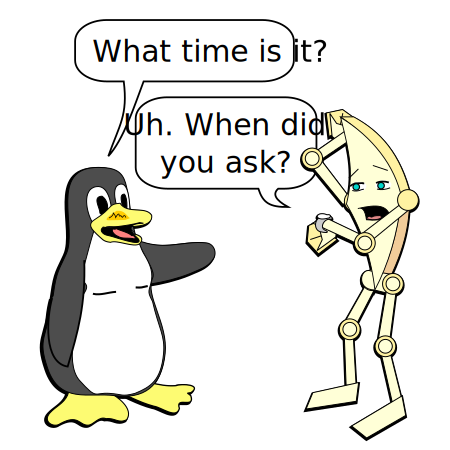
\includegraphics{cartoons/r-2014-What-time-is-it}}
\caption{What Time Is It?}
\ContributedBy{Figure}{fig:app:questions:What Time Is It?}{Melissa Broussard}
\end{figure}

멀티코어 컴퓨터 시스템에서의 시간 관리에서의 핵심적 문제가
\cref{fig:app:questions:What Time Is It?} 로 그려져 있습니다.
한가지 문제는 시간을 읽는데 시간이 걸린다는 겁니다.
어떤 명령은 하드웨어 시계를 읽을거고, 이 읽기 오퍼레이션을 완료하기 위해
off-core (더 나쁜 경우 off-socket) 으로 나가야 할수도 있습니다.
읽혀진 값에 대한 어떤 연산을 해야할 수도 있는데, 예를 들어 요구된 포맷으로
변환하기 위해, network time protocol (NTP) 조정을 위해, 등등이 있겠습니다.
그러니 결국 반환된 시간은 초래된 시간 간격의 시작, 끝, 또는 그 사이 어디에
맞춰져 있을까요?

더 나쁜게, 시간을 읽는 쓰레드는 인터럽트 당하거나 preemption 당할 수도
있습니다.
더 나아가, 시간을 읽는 시점과 그 시간의 실제 사용 사이에 어떤 연산이 있을
겁니다.
이 두개의 가능성 모두 이 불확정 시간을 늘립니다.

\iffalse

A key issue with timekeeping on multicore computer systems is illustrated
by \cref{fig:app:questions:What Time Is It?}.
One problem is that it takes time to read out the time.
An instruction might read from a hardware clock, and might
have to go off-core (or worse yet, off-socket) to complete
this read operation.
It might also be necessary to do some computation on the value read out,
for example, to convert it to the desired format, to apply network time
protocol (NTP) adjustments, and so on.
So does the time eventually returned correspond to the beginning of
the resulting time interval, the end, or somewhere in between?

Worse yet, the thread reading the time might be interrupted or preempted.
Furthermore, there will likely be some computation between reading out
the time and the actual use of the time that has been read out.
Both of these possibilities further extend the interval of uncertainty.

\fi

한가지 방법은 시간을 두번 읽고 타임스탬프가 만들어지는 이 오퍼레이션의 각 방향
중 하나에 있는, 이 두 읽기의 수치적 중간값을 사용하는 것입니다.
그럼 이 두 읽기 사이의 차이는 중간의 오퍼레이션이 수행된 시간의 불확정성의
측정값이 됩니다.

물론, 많은 경우 정확한 시간이 필요합니다.
예를 들어, 인간 사용자의 이익을 위한 시간을 출력하는 경우, 우린 내부의
하드웨어와 소프트웨어 지연이 쓸모없어지는 인간의 느린 반사속도에 기댈 수
있습니다.
비슷하게, 어떤 서버가 클라이언트로의 응답에 시간을 기록해야 한다면, 요청의
도착과 응답의 전송 사이 어느 시간이든 잘 동작할 겁니다.

\iffalse

One approach is to read the time twice, and take the arithmetic mean
of the two readings, perhaps one on each side of the operation being
timestamped.
The difference between the two readings is then a measure of uncertainty
of the time at which the intervening operation occurred.

Of course, in many cases, the exact time is not necessary.
For example, when printing the time for the benefit of a human user,
we can rely on slow human reflexes to render internal hardware and
software delays irrelevant.
Similarly, if a server needs to timestamp the response to a client, any
time between the reception of the request and the transmission of the
response will do equally well.

\fi

% @@@ Scheduling ticks

% @@@ Tickless operation

% @@@ Timers

% @@@ Current time, monotonic operation

% @@@ The many ways in which time can appear to go backwards

% @@@ Causality, the only real time in SMP (or distributed) systems


% appendix/whymb/whymemorybarriers.tex
% mainfile: ../../perfbook.tex
% SPDX-License-Identifier: CC-BY-SA-3.0

\QuickQuizChapter{chp:app:whymb:Why Memory Barriers?}{Why Memory Barriers?}{qqzwhymb}
%
\Epigraph{Order!
	  Order in the court!}
	 {\emph{Unknown}}

그래서 뭐가 CPU 설계자들을 불쌍한 의심없던 SMP 소프트웨어 설계자들에게
memory barreir 를 가하게 홀렸을까요?

짧게 말하자면, 메모리 참조를 재배치 하는 것은 훨씬 나은 성능을 가능하게
하며, 따라서 메모리 배리어는 올바른 오퍼레이션이 순서 맞춰진 메모리 참조에
의존적인 동기화 기능들 같은 것을 위해 순서를 강제하기 위해 필요합니다.

\iffalse

So what possessed CPU designers to cause them to inflict memory barriers
on poor unsuspecting SMP software designers?

In short, because reordering memory references allows much better performance,
and so memory barriers are needed to force ordering in things like
synchronization primitives whose correct operation depends on ordered
memory references.

\fi

이 질문에 대한 더 자세한 답은 CPU 캐쉬가 어떻게 동작하는지, 특히 캐쉬가 정말로
잘 동작하기 위해 무엇을 필요로 하는지에 대한 좋은 이해가 필요합니다.
다음 섹션들은:
\begin{enumerate}
\item	캐쉬의 구조를 보이고,
\item	캐쉬 일관성 프로토콜이 어떻게 CPU 들이 각 메모리 위치의 값에 동의를
	하는 것을 보장하는지 설명하며, 마지막으로
\item	스토어 버퍼와 무효화 큐가 어떻게 캐쉬와 캐쉬 일관성 프로토콜에게 높은
	성능을 이루게 돕는지 설명합니다.
\end{enumerate}
우린 메모리 배리어가 좋은 성능과 확장성을 가능하게 하기 위해 필요하며 CPU 는
그것들과 그것들이 접근하고자 하는 메모리 사이의 연결부보다 수십수백배 빠르다는
사실에서 기인한 필요한 악마임을 보게 될 겁니다.

\iffalse

Getting a more detailed answer to this question requires a good understanding
of how CPU caches work, and especially what is required to make
caches really work well.
The following sections:
\begin{enumerate}
\item	present the structure of a cache,
\item	describe how cache-coherency protocols ensure that CPUs agree
	on the value of each location in memory, and, finally,
\item	outline how store buffers and invalidate queues help
	caches and cache-coherency protocols achieve high performance.
\end{enumerate}
We will see that memory barriers are a necessary evil that is required
to enable good performance and scalability, an evil that stems from
the fact that CPUs are orders of magnitude faster than are both the
interconnects between them and the memory they are attempting to access.

\fi

\section{Cache Structure}
\label{sec:app:whymb:Cache Structure}

현대의 CPU 는 현대의 메모리 시스템보다 훨씬 빠릅니다.
2006년의 CPU 는 나노세컨드당 열개의 명령을 수행할 수도 있으나, 메인 메모리에서
데이터 항목을 가져오는데에는 수십 나노세컨드를 필요로 합니다.
이 속도에서의 괴리---수백배 이상의---는 현대 CPU 에서 찾아볼 수 있는 수백
메가바이트 캐쉬를 초래했습니다.
이 캐쉬들은
\cref{fig:app:whymb:Modern Computer System Cache Structure}
에 보인 것처럼 CPU 들과 연관되어지며, 보통 수 사이클만에 접근될 수
있습니다.\footnote{
	작은 레벨 1 의 캐쉬를 1 사이클 액세스 시간을 가질 만큼 CPU 에 가깝게,
	더 큰 레벨 2 의 캐쉬를 더 긴 액세스 속도, 대략 10 클락 사이클로
	위치하는 식의 다중 레벨의 캐쉬를 사용하는 것은 표준적인 방법입니다.
	고성능 CPU 들은 종종 3 또는 4 레벨의 캐쉬조차 같습니다.}

\iffalse

Modern CPUs are much faster than are modern memory systems.
A 2006 CPU might be capable of executing ten instructions per nanosecond,
but will require many tens of nanoseconds to fetch a data item from
main memory.
This disparity in speed---more than two orders of magnitude---has
resulted in the multi-megabyte caches found on modern CPUs.
These caches are associated with the CPUs as shown in
\cref{fig:app:whymb:Modern Computer System Cache Structure},
and can typically be accessed in a few cycles.\footnote{
	It is standard practice to use multiple levels of cache,
	with a small level-one cache close to the CPU with
	single-cycle access time, and a larger level-two cache
	with a longer access time, perhaps roughly ten clock cycles.
	Higher-performance CPUs often have three or even four levels
	of cache.}

\fi

\begin{figure}
\centering
\resizebox{3in}{!}{\includegraphics{appendix/whymb/cacheSC}}
\caption{Modern Computer System Cache Structure}
\label{fig:app:whymb:Modern Computer System Cache Structure}
\end{figure}

데이터는 ``캐쉬 라인'' 이라 불리는 고정 길이 블록으로 CPU 들의 캐쉬와
메모리 사이를 떠다니는데, 그 크기는 보통 2 의 승수이며, 16 에서 256 바이트
사이를 오갑니다.
어떤 데이터 항목이 어떤 CPU 에 의해 처음 액세스 될 때, 이는 해당 CPU 의 캐쉬에
존재하지 않을 텐데, 이는 ``캐쉬 미스 (cache miss)'' (또는, 더 구체적으로는
``startup'' 또는 ``warmup'' 캐쉬 미스) 가 일어났음을 의미합니다.
이 캐쉬 미스는 이 CPU 가 해당 항목이 메모리로부터 읽어들여지기까지 수백
사이클을 기다려야 (또는 ``stall'' 되어야) 함을 의미합니다.
그러나, 이 항목은 이 CPU 의 캐쉬로 읽혀들여질 것이므로, 뒤따르는 액세스들은 이
항목을 캐쉬에서 발견하고 따라서 완전한 속도를 낼 수 있을 겁니다.

어느정도 시간이 지나면 이 CPU 의 캐쉬는 가득찰 테고, 뒤따르는 미스들은 새로
읽어온 항목을 위한 공간을 마련하기 위해 존재하는 항목을 내버려야 할 겁니다.
이런 캐쉬 미스는 ``capacity miss'' 라고
명명되는데, 캐쉬의 제한된 용량 때문에 일어났기 때문입니다.
그러나, 대부분의 캐쉬는 완전히 가득 차지 않았을 때 조차도 새 항목을 위한 공간을
위해 오래된 항목을 버려야 할 수 있습니다.
이는 커다란 캐쉬는
\cref{fig:app:whymb:CPU Cache Structure} 에 보인 것처럼
고정 크기 해쉬 버킷과 (또는 CPU 설계자들이 부르는 대로라면 ``set'') 체이닝
없는 하드웨어 해쉬 테이블로 구현되어있다는 사실 때문입니다.

\iffalse

Data flows among the CPUs' caches and memory in fixed-length blocks
called ``cache lines'', which are normally a power of two in size,
ranging from 16 to 256 bytes.
When a given data item is first accessed by a given CPU, it will
be absent from that CPU's cache, meaning that a ``cache miss''
(or, more specifically, a ``startup'' or ``warmup'' cache miss)
has occurred.
The cache miss means that the CPU will
have to wait (or be ``stalled'') for hundreds of cycles while the
item is fetched from memory.
However, the item will be loaded into that CPU's cache, so that
subsequent accesses will find it in the cache and therefore run
at full speed.

After some time, the CPU's cache will fill, and subsequent
misses will likely need to eject an item from the cache in order
to make room for the newly fetched item.
Such a cache miss is termed a ``capacity miss'', because it is caused
by the cache's limited capacity.
However, most caches can be forced to eject an old item to make room
for a new item even when they are not yet full.
This is due to the fact that large caches are implemented as hardware
hash tables with fixed-size hash buckets (or ``sets'', as CPU designers
call them) and no chaining, as shown in
\cref{fig:app:whymb:CPU Cache Structure}.

\fi

이 캐쉬는 16개의 ``set'' 과 두개의 ``way'' 를 가져 총 32 개의 ``라인'' 을
가지며, 각 항목은 256 바이트의 정렬된 메모리 블록인 256-바이트 ``캐쉬 라인'' 을
갖습니다.
이 캐쉬 라인 크기는 약간 큰 크기이지만 16 진수 계산을 훨씬 간단하게 해줄
겁니다.
하드웨어 용어에서, 이는 2-way set-associative 캐쉬라 불리며, 16개의 버킷을 갖고
각 버킷의 해쉬 체인은 최대 두개의 원소로 제한된 소프트웨어 해쉬 테이블과
유사합니다.
이 크기 (이 경우 32 캐쉬 라인) 와 associativity (이 경우 2) 는 합쳐져서 이
캐쉬의 ``geometry'' 라고 불립니다.
이 캐쉬는 하드웨어로 구현되었으므로, 그 해쉬 함수는 굉장히 간단합니다:
메모리 주소에서 4개 비트를 꺼냅니다.

\iffalse

This cache has sixteen ``sets'' and two ``ways'' for a total of 32
``lines'', each entry containing a single 256-byte ``cache line'',
which is a 256-byte-aligned block of memory.
This cache line size is a little on the large size, but makes the hexadecimal
arithmetic much simpler.
In hardware parlance, this is a two-way set-associative cache, and
is analogous to a software hash table with
sixteen buckets, where each bucket's hash chain is limited to
at most two elements.
The size (32 cache lines in this case) and the associativity (two in
this case) are collectively called the cache's ``geometry''.
Since this cache is implemented in hardware, the hash function is
extremely simple: extract four bits from the memory address.

\fi

\begin{figure}
\centering
\small
\begin{picture}(170,170)(0,0)

	% Addresses

	\put(0,0){\makebox(20,10){\tt 0xF}}
	\put(0,10){\makebox(20,10){\tt 0xE}}
	\put(0,20){\makebox(20,10){\tt 0xD}}
	\put(0,30){\makebox(20,10){\tt 0xC}}
	\put(0,40){\makebox(20,10){\tt 0xB}}
	\put(0,50){\makebox(20,10){\tt 0xA}}
	\put(0,60){\makebox(20,10){\tt 0x9}}
	\put(0,70){\makebox(20,10){\tt 0x8}}
	\put(0,80){\makebox(20,10){\tt 0x7}}
	\put(0,90){\makebox(20,10){\tt 0x6}}
	\put(0,100){\makebox(20,10){\tt 0x5}}
	\put(0,110){\makebox(20,10){\tt 0x4}}
	\put(0,120){\makebox(20,10){\tt 0x3}}
	\put(0,130){\makebox(20,10){\tt 0x2}}
	\put(0,140){\makebox(20,10){\tt 0x1}}
	\put(0,150){\makebox(20,10){\tt 0x0}}

	% Way 0

	\put(20,163){\makebox(80,10){Way 0}}
	\put(20,0){\framebox(80,10){\tt }}
	\put(20,10){\framebox(80,10){\tt 0x12345E00}}
	\put(20,20){\framebox(80,10){\tt 0x12345D00}}
	\put(20,30){\framebox(80,10){\tt 0x12345C00}}
	\put(20,40){\framebox(80,10){\tt 0x12345B00}}
	\put(20,50){\framebox(80,10){\tt 0x12345A00}}
	\put(20,60){\framebox(80,10){\tt 0x12345900}}
	\put(20,70){\framebox(80,10){\tt 0x12345800}}
	\put(20,80){\framebox(80,10){\tt 0x12345700}}
	\put(20,90){\framebox(80,10){\tt 0x12345600}}
	\put(20,100){\framebox(80,10){\tt 0x12345500}}
	\put(20,110){\framebox(80,10){\tt 0x12345400}}
	\put(20,120){\framebox(80,10){\tt 0x12345300}}
	\put(20,130){\framebox(80,10){\tt 0x12345200}}
	\put(20,140){\framebox(80,10){\tt 0x12345100}}
	\put(20,150){\framebox(80,10){\tt 0x12345000}}

	% Way 1

	\put(100,163){\makebox(80,10){Way 1}}
	\put(100,0){\framebox(80,10){\tt }}
	\put(100,10){\framebox(80,10){\tt 0x43210E00}}
	\put(100,20){\framebox(80,10){\tt }}
	\put(100,30){\framebox(80,10){\tt }}
	\put(100,40){\framebox(80,10){\tt }}
	\put(100,50){\framebox(80,10){\tt }}
	\put(100,60){\framebox(80,10){\tt }}
	\put(100,70){\framebox(80,10){\tt }}
	\put(100,80){\framebox(80,10){\tt }}
	\put(100,90){\framebox(80,10){\tt }}
	\put(100,100){\framebox(80,10){\tt }}
	\put(100,110){\framebox(80,10){\tt }}
	\put(100,120){\framebox(80,10){\tt }}
	\put(100,130){\framebox(80,10){\tt }}
	\put(100,140){\framebox(80,10){\tt }}
	\put(100,150){\framebox(80,10){\tt }}

\end{picture}
\caption{CPU Cache Structure}
\label{fig:app:whymb:CPU Cache Structure}
\end{figure}

\Cref{fig:app:whymb:CPU Cache Structure} 에서, 각 상자는 256-바이트 캐쉬 라인을
가질 수 있는 캐쉬 항목에 연관됩니다.
그러나, 캐쉬 항목은 이 그림의 빈 상자로 표시되어 있듯 비어있을 수 있습니다.
나머지 상자들은 그것들이 가진 캐쉬 라인의 메모리 주소로 표시되어 있습니다.
캐쉬 라인은 256 바이트로 정렬되어 있어야 하므로, 각 주소의 아래쪽 8 비트는 0
이며, 하드웨어 해쉬 함수는 그보다 높은 쪽 4개의 비트를 해쉬 라인 숫자와
매치되게 합니다.

\iffalse

In \cref{fig:app:whymb:CPU Cache Structure},
each box corresponds to a cache entry, which
can contain a 256-byte cache line.
However, a cache entry can be empty, as indicated by the empty boxes
in the figure.
The rest of the boxes are flagged with the memory address of the cache line
that they contain.
Since the cache lines must be 256-byte aligned, the low eight bits of
each address are
zero, and the choice of hardware hash function means that the next-higher
four bits match the hash line number.

\fi

이 그림에 보여진 상황은 프로그램의 코드가 주소 0x43210E00 부터 0x43210EFF 에
위치하고, 이 프로그램이 0x12345000 부터 0x12345EFF 의 데이터를 순차적으로
액세스 했을 때 일어날 수도 있을 겁니다.
이 프로그램이 이제 0x12345F00 을 액세스 하려 한다고 해봅시다.
이 위치는 라인 0xF 로 해쉬 되며, 이 라인의 두 way 는 비어있으므로, 연관된
256-바이트 라인이 수용될 수 있습니다.
이 프로그램이 라인 0x0 으로 해쉬 되는 0x1233000 위치를 접근하려 한다면, 연관된
256-바이트 캐쉬 라인이 way 1 에 수용될 수 있습니다.256-바이트 캐쉬 라인이 way 1
에 수용될 수 있습니다.
그러나, 프로그램이 라인 0xE 로 해쉬되는 0x1233E00 위치를 액세스 하려 하면, 이
새로운 캐쉬 라인을 위한 고간을 만들기 위해 존재하는 라인 중 하나가 버려져야
합니다.
이 버려진 라인이 나중에 다시 액세스 된다면 캐쉬 미스가 일어날 겁니다.
그런 캐쉬 미스는 ``associativity miss'' 라 불립니다.

\iffalse

The situation depicted in the figure might arise if the program's code
were located at address 0x43210E00 through 0x43210EFF, and this program
accessed data sequentially from 0x12345000 through 0x12345EFF\@.
Suppose that the program were now to access location 0x12345F00.
This location hashes to line 0xF, and both ways of this line are
empty, so the corresponding 256-byte line can be accommodated.
If the program were to access location 0x1233000, which hashes to line
0x0, the corresponding 256-byte cache line can be accommodated in
way 1.
However, if the program were to access location 0x1233E00, which hashes
to line 0xE, one of the existing lines must be ejected from the cache
to make room for the new cache line.
If this ejected line were accessed later, a cache miss would result.
Such a cache miss is termed an ``associativity miss''.

\fi

지금까지는 CPU 가 데이터를 읽는 경우만 생각해 봤습니다.
쓰기를 할때는 무슨 일이 일어날까요?
모든 CPU 가 어떤 데이터 항목의 값에 대해 동의한느 것은 중요하므로, 어떤 CPU 는
어떤 데이터 항목에 쓰기를 하기 전에 먼저 그것이 다른 CPU 들의 캐쉬에서
없어지거나 ``무효화 (invalidate)'' 되게 해야만 합니다.
이 무효화가 완료되면, 이 CPU 는 안전하게 데이터 항목을 수정할 수 있습니다.
이 데이터 항목이 이 CPU 의 캐쉬에 존재하지만 읽기 전용이었다면, 이 과정은
``write miss'' 라고 불립니다.
특정 CPU 가 다른 CPU 들의 캐쉬로부터 특정 데이터 항목을 완전히 무효화 하면,
해당 CPU 는 이 데이터 ㅎ아목을 반복적으로 쓸 수 (그리고 읽을 수) 있을 겁니다.

\iffalse

Thus far, we have been considering only cases where a CPU reads
a data item.
What happens when it does a write?
Because it is important that all CPUs agree on the value of a given
data item, before a given CPU writes to that data item, it must first
cause it to be removed, or ``invalidated'', from other CPUs' caches.
Once this invalidation has completed, the CPU may safely modify the
data item.
If the data item was present in this CPU's cache, but was read-only,
this process is termed a ``write miss''.
Once a given CPU has completed invalidating a given data item from other
CPUs' caches, that CPU may repeatedly write (and read) that data item.

\fi

나중에 다른 CPU 들 중 하나가 이 데이터 항목을 접근하려 하면 캐쉬 미스가 일어날
텐데, 이번엔 이 앞의 CPU 가 그 항목에 쓰기를 하기 위해 무효화를 했기
때문입니다.
이런 종류의 캐쉬 미스는 ``communication miss'' 라 불리는데, 이는 보통 CPU 들이
이 데이터 항목을 통신을 위해 사용하기 때문입니다 (예를 들면, 락은 CPU 들 사이에
상호 배타 알고리즘을 통신하기 위해 사용되는 데이터 항목입니다).

분명하게, 모든 CPU 가 데이터의 일관된 시선을 유지하게 보장하는 데에는 큰 주의가
필요합니다.
이 모든 읽기, 무효화, 그리고 쓰기를 놓고 볼 때, 데이터가 손실되거나 (아마도 더
나쁘게도) 다른 CPU 들이 같은 데이터 항목에 대해 그들의 캐쉬에서는 다른 값을
갖고 있는 경우를 상상하기는 쉽습니다.
이 문제들은 ``캐쉬 일관성 프로토콜'' 에 의해 방지되는데, 다음 섹션에서
설명합니다.

\iffalse

Later, if one of the other CPUs attempts to access the data item, it
will incur a cache miss, this time because the first CPU invalidated
the item in order to write to it.
This type of cache miss is termed a ``communication miss'', since it
is usually due to several CPUs using the data items to communicate
(for example, a lock is a data item that is used to communicate among
CPUs using a mutual-exclusion algorithm).

Clearly, much care must be taken to ensure that all CPUs maintain
a coherent view of the data.
With all this fetching, invalidating, and writing, it is easy to
imagine data being lost or (perhaps worse) different CPUs having
conflicting values for the same data item in their respective
caches.
These problems are prevented by ``cache-coherency protocols'',
described in the next section.

\fi

\section{Cache-Coherence Protocols}
\label{sec:app:whymb:Cache-Coherence Protocols}

캐쉬 일관성 프로토콜은 비일관적이거나 손실된 데이터를 막을 수 있게끔 캐쉬 라인
상태들을 관리합니다.
이 프로토콜은 수십개의 상태를 가질 정도로\footnote{
	Culler 등의 책~\cite{DavidECuller1999} 의 670 과 671 페이지에서 각각
	SGI Origin2000 과 Sequent (지금은 IBM) NUMA-Q 를 위한 9개 상태와 26개
	상태 다이어그램들을 보시기 바랍니다.
	두 다이어그램은 실제의 것보다 훨씬 간단합니다.}
매우 복잡할 수 있으나 우리의 목적을 위해선 4개 상태의 MESI 캐쉬 일관성
프로토콜에 대해서만 걱정하면 됩니다.

\iffalse

Cache-coherency protocols manage cache-line states so as to prevent
inconsistent or lost data.
These protocols can be quite complex, with many tens
of states,\footnote{
	See Culler et al.~\cite{DavidECuller1999} pages 670 and 671
	for the nine-state and 26-state diagrams for SGI Origin2000
	and Sequent (now IBM) NUMA-Q, respectively.
	Both diagrams are significantly simpler than real life.}
but for our purposes we need only concern ourselves with the
four-state MESI cache-coherence protocol.

\fi

\subsection{MESI States}
\label{sec:app:whymb:MESI States}

MESI 는 ``modified'', ``exclusive'', ``shared`, 그리고 ``invalid'' 라는 각 캐쉬
라인이 이 프로토콜을 사용해 취할 수 있는 네개의 상태를 의미합니다.
따라서 이 프로토콜을 사용하는 캐쉬는 각 캐쉬 라인에 해당 라인의 물리 주소와
데이터에 더해 2 비트의 상태 ``tag'' 를 유지합니다.

``modified'' 상태의 라인은 연관된 CPU 로부터의 최근의 메모리 스토어를 의미하며,
이 연관된 메모리는 다른 CPU 의 캐쉬에는 보이지 않을 것이 보장됩니다.
따라서 ``modified'' 상태의 캐쉬 라인은 이 CPU 에 ``owned (소유되어 있다)'' 라고
말해집니다.
이 캐쉬는 데이터의 최신 복사본만을 쥐고 있으므로, 이 캐쉬는 궁극적으로는 이를
메모리에 다시 쓰거나 다른 캐쉬에게 넘겨줄 책임을 가지며, 이는 이 라인이 다른
데이터를 잡아두기 위해 재사용되기 전에 행해져야만 합니다.

\iffalse

MESI stands for ``modified'', ``exclusive'', ``shared'', and ``invalid'',
the four states a given cache line can take on using this
protocol.
Caches using this protocol therefore maintain a two-bit state ``tag'' on each
cache line in addition to that line's physical address and data.
% cite Schimmel's book on virtual caches.

A line in the ``modified'' state has been subject to a recent memory store
from the corresponding CPU, and the corresponding memory is guaranteed
not to appear in any other CPU's cache.
Cache lines in the ``modified'' state can thus be said to be ``owned''
by the CPU\@.
Because this cache holds the only up-to-date copy of the data, this
cache is ultimately responsible for either writing it back to memory
or handing it off to some other cache, and must do so before reusing
this line to hold other data.

\fi

``exclusive'' 상태는 ``modified'' 상태와 매우 비슷한데, 한가지 예외는 이 캐쉬
라인은 아직 연관된 CPU 에 의해 수정되지 않았다는 것으로, 이는 결국 메모리에
위치해 있는 이 캐쉬 라인의 데이터의 복사본도 최신의 것이라는 겁니다.
그러나, 이 CPU 는 언제든 이 라인에 스토어를 행할 수 있으므로, 다른 CPU 에게
물어보지 않고서는 ``exclusive'' 상태의 라인은 연관된 CPU 에게 소유되어 있다고
말해질 수 있습니다.
그러나, 메모리의 연관된 값이 최신의 것이기 때문에, 이 캐쉬는 이 데이터를
메모리에 다시 쓰거나 다른 CPU 에게 넘겨주지 않고도 버릴 수 있습니다.

``shared'' 상태의 라인은 최소 하나의 다른 CPU 의 캐쉬에 복사되어 있을 수도
있어서, 이 CPU 는 다른 CPU 에게 자문을 먼저 구하지 않고는 이 라인에 스토어를 할
수 없습니다.
``exclusive'' 상태에서와 마찬가지로, 메모리에 있는 이 연관된 값은 최신의
것이어서, 이 캐쉬는 이 데이터를 메모리에 다시 쓰거나 다른 CPU 에게 넘겨주지
않고도 버릴 수 있습니다.

\iffalse

The ``exclusive'' state is very similar to the ``modified'' state,
the single exception being that the cache line has not yet been
modified by the corresponding CPU, which in turn means that the
copy of the cache line's data that resides in memory is up-to-date.
However, since the CPU can store to this line at any time, without
consulting other CPUs, a line in the ``exclusive'' state can still
be said to be owned by the corresponding CPU\@.
That said, because the corresponding value in memory is up to date,
this cache can discard this data without writing it back to memory
or handing it off to some other CPU\@.

A line in the ``shared'' state might be replicated in at least
one other CPU's cache, so that this CPU is not permitted to store
to the line without first consulting with other CPUs.
As with the ``exclusive'' state, because the corresponding value
in memory is up to date,
this cache can discard this data without writing it back to memory
or handing it off to some other CPU\@.

\fi

``invalid'' 상태의 라인은 비어 있는데, 달리 말해 데이터를 쥐고 있지 않습니다.
캐쉬에 새 데이터가 들어오면, 이는 가능하다면 ``invalid'' 상태의 캐쉬 라인에
위치하게 됩니다.
다른 상태의 라인을 교체하는 것은 교체된 라인이 미래에 참조될 때 비용이 높은
캐쉬 미스를 초래하기 때문에 이 방법이 선호됩니다.

모든 CPU 는 캐쉬 라인들로 운반되는 데이터에 대해 일관된 모습을 봐야만 하므로,
이 캐쉬 일관성 프로토콜은 시스템을 돌아다니는 캐쉬 라인들의 움직임을 조정하는
메세지를 제공합니다.

\iffalse

A line in the ``invalid'' state is empty, in other words, it holds
no data.
When new data enters the cache, it is placed into a
cache line that was in the ``invalid'' state if possible.
This approach is preferred because replacing a line in any other
state could result in an expensive cache miss should the replaced
line be referenced in the future.

Since all CPUs must maintain a coherent view of the data carried in
the cache lines, the cache-coherence protocol provides messages
that coordinate the movement of cache lines through the system.

\fi

\subsection{MESI Protocol Messages}
\label{sec:app:whymb:MESI Protocol Messages}

앞의 섹션에 설명된 많은 변환은 CPU 들 사이의 통신을 필요로 합니다.
CPU 들이 하나의 공유 버스에 있다면, 다음 메세지가 충분합니다:

\iffalse

Many of the transitions described in the previous section require
communication among the CPUs.
If the CPUs are on a single shared bus, the following messages suffice:

\fi

\begin{description}[style=nextline]
\item	[Read:]
	``Read'' 메세지는 읽혀질 캐쉬 라인의 물리 주소를 담습니다.
\item	[Read Response:]
	``Read response'' 메세지는 앞의 ``read'' 메세지에 의해 요청된 데이터를
	담습니다.
	이 ``read response'' 메세지는 메모리 또는 다른 캐쉬들 가운데 하나에
	의해 제공될 수도 있습니다.
	예를 들어, 캐쉬들 가운데 하나가 ``modified'' 상태로 해당 데이터를
	가지고 있다면, 그 캐쉬는 ``read response'' 메세지를 제공해야만 합니다.
\item	[Invalidate:]
	``Invalidate'' 메세지는 무효화 될 캐쉬 라인의 물리 주소를 담습니다.
	모든 다른 캐쉬들은 그들의 캐쉬에서 연관된 데이터를 제거하고 응답해야만
	합니다.
\item	[Invalidate Acknowledge:]
	``Invalidate'' 메세지를 받는 CPU 는 자신의 캐쉬에서 명시된 데이터를
	제거한 후 ``invalidate acknowledge'' 메세지를 가지고 응답해야만 합니다.

\iffalse

\item	[Read:]
	The ``read'' message contains the physical address of the cache line
	to be read.
\item	[Read Response:]
	The ``read response'' message contains the data requested by an
	earlier ``read'' message.
	This ``read response'' message might be supplied either by
	memory or by one of the other caches.
	For example, if one of the caches has the desired data in
	``modified'' state, that cache must supply the ``read response''
	message.
\item	[Invalidate:]
	The ``invalidate'' message contains the physical address of the
	cache line to be invalidated.
	All other caches must remove the corresponding data from their
	caches and respond.
\item	[Invalidate Acknowledge:]
	A CPU receiving an ``invalidate'' message must respond with an
	``invalidate acknowledge'' message after removing the specified
	data from its cache.

\fi

\item	[Read Invalidate:]
	``Read invalidate'' 메세지는 읽혀질 캐쉬 라인의 물리 주소를 담고
	있으며, 동시에 다른 캐쉬들이 이 데이터를 제거하게 지시합니다.
	따라서, 이는 그 이름이 암시하듯 ``read'' 와 ``invalidate'' 의
	조합입니다.
	``Read invalidate'' 메세지는 그에 대한 응답으로 ``read response'' 와
	``invalidate acknowledge'' 메세지의 집합을 모두 요구합니다.
\item	[Writeback:]
	``Writeback'' 메세지는 메모리에 도로 쓰여질 (그리고 아마도 다른 CPU 의
	캐쉬에도 기어들어가게 될--``snooped''--) 주소와 데이터를 포함합니다.
	이 메세지는 캐쉬들이 다른 데이터를 위한 공간을 만들기 위해 ``modified''
	상태의 라인을 제거하는 걸 가능하게 합니다.

\iffalse

\item	[Read Invalidate:]
	The ``read invalidate'' message contains the physical address
	of the cache line to be read, while at the same time directing
	other caches to remove the data.
	Hence, it is a combination of a ``read'' and an ``invalidate'',
	as indicated by its name.
	A ``read invalidate'' message requires both a ``read response''
	and a set of ``invalidate acknowledge'' messages in reply.
\item	[Writeback:]
	The ``writeback'' message contains both the address and the
	data to be written back to memory (and perhaps ``snooped''
	into other CPUs' caches along the way).
	This message permits caches to eject lines in the ``modified''
	state as needed to make room for other data.

\fi

\end{description}

\QuickQuiz{
	Writeback 메세지는 어디서 생겨나서 어디로 향하게 되나요?

	\iffalse

	Where does a writeback message originate from and where does
	it go to?

	\fi

}\QuickQuizAnswer{
	Writeback 메세지는 특정 CPU 에서, 어떤 설계에서는 특정 CPU 의 캐쉬의
	특정 레벨에서---또는 심지어 여러 CPU 들에 공유되어 있는 캐쉬에서도---
	생성됩니다.
	핵심은 특정 캐쉬가 특정 데이터 항목을 위한 공간이 없으며, 따라서 공간을
	만들기 위해 이 캐쉬에서 어떤 데이터 조각들이 제거되야 한다는 겁니다.
	메모리나 다른 캐쉬에 복사되어 있는 데이터 조각이 존재한다면 그 조각은
	writeback 메세지의 필요 없이 단순히 폐기될 수 있을 겁니다.

	다른 한편, 만약 제거될 수 있는 모든 데이터 조각이 modified 상태여서
	유일한 최신 상태의 데이터 복사본은 이 캐쉬에만 있다면, 이 데이터 항목들
	가운데 하나는 어딘가 다른곳에 복사되어야만 합니다.
	이 복사 오퍼레이션은 ``witeback message'' 를 사용해 취해집니다.

	\iffalse

	The writeback message originates from a given CPU, or in some
	designs from a given level of a given CPU's cache---or even
	from a cache that might be shared among several CPUs.
	The key point is that a given cache does not have room for
	a given data item, so some other piece of data must be ejected
	from the cache to make room.
	If there is some other piece of data that is duplicated in some
	other cache or in memory, then that piece of data may be simply
	discarded, with no writeback message required.

	On the other hand, if every piece of data that might be ejected
	has been modified so that the only up-to-date copy is in this
	cache, then one of those data items must be copied somewhere
	else.
	This copy operation is undertaken using a ``writeback message''.

	\fi

	Writeback 메세지의 목적지는 이 새 값을 저장할 어딘가가 됩니다.
	이는 메인 메모리일 수도 있으나, 다른 캐쉬일 수도 있습니다.
	그게 캐쉬라면, 이는 보통 같은 CPU 를 위한 더 높은 레벨의 캐쉬인데, 예를
	들어 level-1 캐쉬는 level-2 캐쉬로 도로 쓰기를 할수도 있습니다.
	그러나, 어떤 하드웨어 설계는 CPU 간 writeback 을 허용해서 CPU~0 의
	캐쉬는 writeback 메세지를 CPU~1 에게 보낼 수도 있습니다.
	이는 일반적으로 예를 들면 최근에 read request 를 보냈다던지 하는 식으로
	CPU~1 이 어떻게든 이 데이터에의 흥미를 알게 된 경우 행해질 겁니다.

	요약하자면, writeback 메세지는 공간이 부족한 시스템의 어느 부분에서
	보내어지며, 이 데이터를 수용할 수 있는 시스템의 어떤 다른 부분에서
	받아지게 됩니다.

	\iffalse

	The destination of the writeback message has to be something
	that is able to store the new value.
	This might be main memory, but it also might be some other cache.
	If it is a cache, it is normally a higher-level cache for the
	same CPU, for example, a level-1 cache might write back to a
	level-2 cache.
	However, some hardware designs permit cross-CPU writebacks,
	so that CPU~0's cache might send a writeback message to CPU~1.
	This would normally be done if CPU~1 had somehow indicated
	an interest in the data, for example, by having recently
	issued a read request.

	In short, a writeback message is sent from some part of the
	system that is short of space, and is received by some other
	part of the system that can accommodate the data.

	\fi

}\QuickQuizEnd

흥미롭게도, 공유 메모리 멀티프로세서 시스템은 장막을 걷어보면 실제로
메세지 전달 (message-passing) 컴퓨터입니다.
이는 분산된 공유 메모리를 사용하는 SMP 머신들의 클러스터는 시스템 구조의 두개의
다른 수준에서의 공유 메모리를 구현하기 위해 메세지 전달을 사용하고 있음을
의미합니다.

\iffalse

Interestingly enough, a shared-memory multiprocessor system really
is a message-passing computer under the covers.
This means that clusters of SMP machines that use distributed shared memory
are using message passing to implement shared memory at two different
levels of the system architecture.

\fi

\QuickQuizSeries{%
\QuickQuizB{
	두개의 CPU 가 동시에 같은 캐쉬 라인을 무효화 하려 하면 어떻게 되나요?

	\iffalse

	What happens if two CPUs attempt to invalidate the
	same cache line concurrently?

	\fi

}\QuickQuizAnswerB{
	해당 CPU 들 가운데 하나가 공유 버스에의 액세스를 먼저 얻고, 그 CPU 가
	``승리'' 합니다.
	다른 CPU 는 자신의 해당 캐쉬 라인 복사본을 무효화 하고 그 다른 CPU 에게
	``invalidate acknowledge'' 메세지를 보내야만 합니다.

	물론, 진 CPU 는 곧바로 ``read invalidate'' 트랜잭션을 요청할 것으로
	예상될 수 있으며, 따라서 승리한 CPU 의 승리는 짧은 것일 겁니다.

	\iffalse

	One of the CPUs gains access
	to the shared bus first,
	and that CPU ``wins''.  The other CPU must invalidate its copy of the
	cache line and transmit an ``invalidate acknowledge'' message
	to the other CPU\@.

	Of course, the losing CPU can be expected to immediately issue a
	``read invalidate'' transaction, so the winning CPU's victory will
	be quite ephemeral.

	\fi

}\QuickQuizEndB
%
\QuickQuizM{
	거대 멀티프로세서에서 ``invalidate'' 메세지가 나타날 때, 모든 CPU 는
	``invalidate acknowledge'' 응답을 보내야만 합니다.
	이로 인한 ``invalidate acknowledge'' 응답의 ``폭풍'' 은 시스템 버스를
	완전히 포화시키지 않을까요?

	\iffalse

	When an ``invalidate'' message appears in a large multiprocessor,
	every CPU must give an ``invalidate acknowledge'' response.
	Wouldn't the resulting ``storm'' of ``invalidate acknowledge''
	responses totally saturate the system bus?

	\fi

}\QuickQuizAnswerM{
	이 거대 규모 멀티프로세서가 실제로 그런 방식으로 구현되어 있다면 그럴
	수도 있습니다.
	특히 NUMA 머신 같은 거대한 멀티프로세서들은 이것을 포함한 문제들을 막기
	위해 ``directory-based'' 캐쉬 일관성 프로토콜이라 불리는 것을
	사용합니다.

	\iffalse

	It might, if large-scale multiprocessors were in fact implemented
	that way.  Larger multiprocessors, particularly NUMA machines,
	tend to use so-called ``directory-based'' cache-coherence
	protocols to avoid this and other problems.

	\fi

}\QuickQuizEndM
%
\QuickQuizE{
	SMP 머신이 정말로 메세지 전달을 어쨌든 사용한다면, 왜 SMP 를 신경쓰죠?

	\iffalse

	If SMP machines are really using message passing
	anyway, why bother with SMP at all?

	\fi

}\QuickQuizAnswerE{
	과거의 수십년간 이 주제에 대한 상당한 논란이 있었습니다.
	한가지 답은 캐쉬 일관성 프로토콜은 상당히 간단하며, 따라서 하드웨어에
	직접 구현될 수 있어서 소프트웨어 메세지 전달로는 얻어질 수 없는
	대역폭과 응답시간 향상을 얻는다는 겁니다.
	또다른 답은 거대 SMP 머신과 작은 SMP 머신의 클러스터의 상대적 가격
	때문에 경제로부터 진실을 찾을 수 있다는 겁니다.
	세번째 답은 SMP 프로그래밍 모델은 분산 시스템의 그것보다 더 사용하기
	쉽다는 것입니다만, 반박론자들은 HPC 클러스터와 MPI 의 등장을 이야기할
	수도 있겠습니다.
	그러므로 토론은 계속됩니다.

	\iffalse

	There has been quite a bit of controversy on this topic over
	the past few decades.  One answer is that the cache-coherence
	protocols are quite simple, and therefore can be implemented
	directly in hardware, gaining bandwidths and latencies
	unattainable by software message passing.  Another answer is that
	the real truth is to be found in economics due to the relative
	prices of large SMP machines and that of clusters of smaller
	SMP machines.  A third answer is that the SMP programming
	model is easier to use than that of distributed systems, but
	a rebuttal might note the appearance of HPC clusters and MPI\@.
	And so the argument continues.

	\fi

}\QuickQuizEndE
}

\subsection{MESI State Diagram}
\label{sec:app:whymb:MESI State Diagram}

특정 캐쉬 라인의 상태는
\cref{fig:app:whymb:MESI Cache-Coherency State Diagram} 에 보인 것처럼 프로토콜
메세지가 보내지고 받아짐에 따라 바뀝니다.

\iffalse

A given cache line's state changes
as protocol messages are sent and received, as
shown in \cref{fig:app:whymb:MESI Cache-Coherency State Diagram}.

\fi

\begin{figure}[htb]
\centering
% \resizebox{3in}{!}{\includegraphics{appendix/whymb/MESI}}
\includegraphics{appendix/whymb/MESI}
\caption{MESI Cache-Coherency State Diagram}
\label{fig:app:whymb:MESI Cache-Coherency State Diagram}
\end{figure}

이 그림에서의 전환 움직임들은 다음과 같습니다:

\iffalse

The transition arcs in this figure are as follows:

\fi

\begin{description}[style=nextline]
\item	[Transition (a):]
	캐쉬 라인이 메모리에 도로 쓰여지나, 이 CPU 는 자신의 캐쉬에 이를
	유지하며 더 나아가 이를 수정할 권리를 유지합니다.
	이 전환은 ``writeback'' 메세지를 필요로 합니다.
\item	[Transition (b):]
	이 CPU 가 이미 배타적 액세스를 가지고 있는 캐쉬 라인에 쓰기를 합니다.
	이 전환은 어떤 메세지도 보내지거나 받아질 필요를 갖지 않습니다.
\item	[Transition (c):]
	이 CPU 가 수정한 캐쉬 라인을 위한 ``read invalidate'' 메세지를
	받습니다.
	이 CPU 는 자신의 지역 복사본을 무효화 하고, 이 데이터를 요청한 CPU 에게
	보내며 자신이 더이상 그 지역 복사본을 가지고 있지 않음을 알리는 ``read
	response'' 와 ``invalidate acknowledge'' 메세지를 응답해야 합니다.

\iffalse

\item	[Transition (a):]
	A cache line is written back to memory, but the CPU retains
	it in its cache and further retains the right to modify it.
	This transition requires a ``writeback'' message.
\item	[Transition (b):]
	The CPU writes to the cache line that it already had exclusive
	access to.
	This transition does not require any messages to be sent or
	received.
\item	[Transition (c):]
	The CPU receives a ``read invalidate'' message for a cache line
	that it has modified.
	The CPU must invalidate its local copy, then respond with both a
	``read response'' and an ``invalidate acknowledge'' message,
	both sending the data to the requesting CPU and indicating
	that it no longer has a local copy.

\fi

\item	[Transition (d):]
	이 CPU 가 자신의 캐쉬에 존재하지 않던 데이터 항목에 대해 어토믹
	read-modify-write 오퍼레이션을 행합니다.
	이는 ``read invalidate'' 를 보내고, ``read response'' 를 통해 그
	데이터를 받습니다.
	이 CPU 는 완전한 ``invalidate acknowledge'' 응답 집합을 받으면 이
	전환을 완료할 수 있습니다.
\item	[Transition (e):]
	이 CPU 가 자신의 캐쉬에 read-only 로 가지고 있던 데이터 항목에 어토믹
	read-modify-write 오퍼레이션을 행합니다.
	이는 ``invalidate'' 메세지를 보내야 하며, 이 전환을 완료하기 전에
	완전한 ``invalidate acknowledge'' 응답 집합을 기다려야 합니다.
\item	[Transition (f):]
	어떤 다른 CPU 가 이 캐쉬 라인을 읽고, 그 데이터가 이 CPU 의 캐쉬에서
	제공되어서, 읽기 전용 복사본을 유지하며, 이를 메모리에 도로 쓰기 할
	수도 있습니다.
	이 전환은 ``read'' 메세지의 도착으로 시작되고, 이 CPU 는 요청된
	데이터를 포함한 ``read response'' 메세지로 응답합니다.

\iffalse

\item	[Transition (d):]
	The CPU does an atomic read-modify-write operation on a data item
	that was not present in its cache.
	It transmits a ``read invalidate'', receiving the data via
	a ``read response''.
	The CPU can complete the transition once it has also received a
	full set of ``invalidate acknowledge'' responses.
\item	[Transition (e):]
	The CPU does an atomic read-modify-write operation on a data item
	that was previously read-only in its cache.
	It must transmit ``invalidate'' messages, and must wait for a
	full set of ``invalidate acknowledge'' responses before completing
	the transition.
\item	[Transition (f):]
	Some other CPU reads the cache line, and it is supplied from
	this CPU's cache, which retains a read-only copy, possibly also
	writing it back to memory.
	This transition is initiated by the reception of a ``read''
	message, and this CPU responds with a ``read response'' message
	containing the requested data.

\fi

\item	[Transition (g):]
	어떤 다른 CPU 가 이 캐쉬 라인의 데이터 항목을 읽고, 그 데이터가 이 CPU
	의 캐쉬 또는 메모리에서 제공됩니다.
	어느 경우든, 이 CPU 는 읽기 전용 복사본을 유지합니다.
	이 전환은 ``read'' 메세지의 도착으로 시작되며, 이 CPU 는 요청된
	데이터를 담은 ``read response'' 메세지를 응답합니다.
\item	[Transition (h):]
	이 CPU 는 이 캐쉬 라인에 어떤 데이터 항목을 곧 써야 할 것임을 깨닫고
	따라서 ``invalidate'' 메세지를 보냅니다.
	이 CPU 는 완전한 ``invalidate acknowledge'' 응답 집합을 받기 전까지는
	이 전환을 끝내지 못합니다.
	대안적으로, 모든 다른 CPU 들이 ``writeback'' 메세지를 통해 이 캐쉬
	라인을 자신들의 캐쉬에서 제거하여 (아마도 다른 캐쉬 라인을 위한 공간을
	만들기 위해) 이 CPU 가 이를 캐쉬에 두는 마지막 CPU 가 되게 할수도
	있습니다.
\item	[Transition (i):]
	어떤 다른 CPU 가 이 CPU 의 캐쉬에만 있는 캐쉬라인의 데이터 항목에 대해
	어토믹 read-modify-write 오퍼레이션을 수행해서, 이 CPU 는 자신의
	캐쉬에서 이 라인을 무효화 합니다.
	이 전환은 ``read invalidate'' 메세지의 도착으로 시작되며, 이 CPU 는
	``read response'' 와 ``invalidate acknowledge'' 메세지를 모두
	응답합니다.

\iffalse

\item	[Transition (g):]
	Some other CPU reads a data item in this cache line,
	and it is supplied either from this CPU's cache or from memory.
	In either case, this CPU retains a read-only copy.
	This transition is initiated by the reception of a ``read''
	message, and this CPU responds with a ``read response'' message
	containing the requested data.
\item	[Transition (h):]
	This CPU realizes that it will soon need to write to some data
	item in this cache line, and thus transmits an ``invalidate'' message.
	The CPU cannot complete the transition until it receives a full
	set of ``invalidate acknowledge'' responses.
	Alternatively, all other CPUs eject this cache line from
	their caches via ``writeback'' messages (presumably to make room
	for other cache lines),
	so that this CPU is the last CPU caching it.
\item	[Transition (i):]
	Some other CPU does an atomic read-modify-write operation on
	a data item in a cache line held only in this CPU's cache,
	so this CPU invalidates it from its cache.
	This transition is initiated by the reception of a ``read invalidate''
	message, and this CPU responds with both a ``read response''
	and an ``invalidate acknowledge'' message.

\fi

\item	[Transition (j):]
	이 CPU 는 자신의 캐쉬에 있지 않던 캐쉬 라인의 데이터 항목에 스토어를
	행하고, 따라서 ``read invalidte'' 메세지를 보냅니다.
	이 CPU 는 ``read response'' 와 완전환 ``invalidate acknowledge'' 메세지
	집합을 받기 전까지 이 전환을 완료할 수 없습니다.
\item	[Transition (k):]
	이 CPU 가 자신의 캐쉬에 없던 캐쉬 라인의 데이터 항목을 로드합니다.
	이 CPU 는 ``read'' 메세지를 보내며, 연관된 ``read response'' 를 받으면
	전환을 완료합니다.
\item	[Transition (l):]
	어떤 다른 CPU 가 이 캐쉬 라인의 데이터 항목으로 스토어를 하지만, 이
	캐쉬 라인은 다른 CPU 의 캐쉬에 (이 현재 CPU 의 캐쉬 같은) 있으므로 이
	캐쉬 라인을 읽기 전용 상태로 유지합니다.
	이 전환은 ``invalidate'' 메세지의 수신으로 시작되며, 이 CPU 는
	``invalidate acknowledge'' 메세지를 응답합니다.

\iffalse

\item	[Transition (j):]
	This CPU does a store to a data item in a cache line that was not
	in its cache, and thus transmits a ``read invalidate'' message.
	The CPU cannot complete the transition until it receives the
	``read response'' and a full set of ``invalidate acknowledge''
	messages.
	The cache line will presumably transition to ``modified'' state via
	transition (b) as soon as the actual store completes.
\item	[Transition (k):]
	This CPU loads a data item in a cache line that was not
	in its cache.
	The CPU transmits a ``read'' message, and completes the
	transition upon receiving the corresponding ``read response''.
\item	[Transition (l):]
	Some other CPU does a store to
	a data item in this cache line, but holds this cache line in read-only
	state due to its being held in other CPUs' caches (such as the
	current CPU's cache).
	This transition is initiated by the reception of an ``invalidate''
	message, and this CPU responds with
	an ``invalidate acknowledge'' message.

\fi

\end{description}

\QuickQuiz{
	하드웨어는 앞서 설명된 지연된 전환을 어떻게 처리하나요?

	\iffalse

	How does the hardware handle the delayed transitions
	described above?

	\fi

}\QuickQuizAnswer{
	일반적으로 상태를 더함으로써 처리합니다만, 이 추가적인 상태는 이 캐쉬
	라인에 정말로 저장될 필요는 없는데, 한번에 몇개의 라인만이 전환되고
	있을 것이라는 사실 덕입니다.
	하지만 전환을 지연해야 하는 필요는 실제 세계의 캐쉬 일관성 프로토콜이
	이 부록에 묘사된 과하게 단순화된 MESI 프로토콜보다 훨씬 더 복잡해지게
	만드는 하나의 문제입니다.
	Hennessy 와 Patterson 의 고전적인 컴퓨터 구조 소개~\cite{Hennessy95a}
	는 이 문제 여럿을 다룹니다.

	\iffalse

	Usually by adding additional states, though these additional
	states need not be actually stored with the cache line, due to
	the fact that only a few lines at a time will be transitioning.
	The need to delay transitions is but one issue that results in
	real-world cache coherence protocols being much more complex than
	the over-simplified MESI protocol described in this appendix.
	Hennessy and Patterson's classic introduction to computer
	architecture~\cite{Hennessy95a} covers many of these issues.

	\fi

}\QuickQuizEnd

\subsection{MESI Protocol Example}
\label{sec:app:whymb:MESI Protocol Example}

이제 초기에는 메모리의 address~0 에 위치해 있는 데이터의 캐쉬 라인이 네개의 CPU
시스템에서의 단일 캐쉬 라인만 갖는 여러 캐쉬들을 이동하는 모습을 캐쉬 라인의
관점에서 봅시다.
\Cref{tab:app:whymb:Cache Coherence Example}
이 이 데이터의 흐름을 보이는데, 첫번째 열은 오퍼레이션의 순서를, 두번째 열은 그
오퍼레이션을 행하는 CPU 를, 세번째 열은 수행되는 오퍼레이션을, 나머지 네개의
열은 각 CPU 의 캐쉬 라인의 상태를 (메모리 주소에 이어 MESI 상태), 그리고 마지막
두개의 열은 연관된 메모리 내용이 최신인지 (``V'') 아닌지 (``I'') 보입니다.

\iffalse

Let's now look at this from the perspective of a cache line's worth
of data, initially residing in memory at address~0,
as it travels through the various single-line direct-mapped caches
in a four-CPU system.
\Cref{tab:app:whymb:Cache Coherence Example}
shows this flow of data, with the first column showing the sequence
of operations, the second the CPU performing the operation,
the third the operation being performed, the next four the state
of each CPU's cache line (memory address followed by MESI state),
and the final two columns whether the corresponding memory contents
are up to date (``V'') or not (``I'').

\fi

처음에는 이 데이터가 위치해 있는 CPU 캐쉬 라인들은 ``invalid'' 상태에 있으며,
그 데이터는 메모리에서 유효합니다.
CPU~0 이 address~0 에서 데이터를 로드하면, 이는 CPU~0 의 캐쉬에 ``shared''
상태로 들어가게 되며, 이는 여전히 메모리에서 유효합니다.
CPU~3  역시 address~0 에서 이 데이터를 로드해서, 두 CPU 의 캐쉬에서 ``shared''
상태로 있게 하며, 이 데이터는 여전히 메모리 상에서 유효합니다.
이어서 CPU~0 이 다른 캐쉬 라인을 (address~8) 로드하는데, 이는 address~0 의
데이터를 무효화를 통해 자신의 캐쉬에서 밖으로 내보내고 address~8 의 데이터로
교체합니다.
CPU~2 가 이제 address~0 으로부터의 로드를 합니다만, 이 CPU 는 자신이 곧 거기에
스토어를 해야 할 것임을 깨달아 배타적 복사본을 얻기 위해 ``read invalidate''
메세지를 사용하여 이를 CPU~3 의 캐쉬에서 무효화 시킵니다 (메모리의 복사본은
여전히 최신의 것으로 남아있지만).
이어서 CPU~2 는 예상된 스토어를 행하여 이 상태를 ``modified'' 로 바꿉니다.
메모리에 있는 이 데이터의 사본은 이제 최신이 아닙니다.
CPU~1 은 원자적 값 증가를 행하는데, CPU~2 의 캐쉬로부터 데이터를 얻고 이를
무효화 하기 위해 ``read invalidate'' 메세지를 사용하며, 따라서 CPU~1 의 캐쉬는
``modified'' 상태가 됩니다 (그리고 메모리의 복사본은 최신이 아닌 상태로
유지됩니다).
마지막으로, CPU~1 이 address~8 의 캐쉬 라인을 읽는데, address~0 의 데이터를
메모리로 도로 내보내기 위해 ``writeback'' 메세지를 사용합니다.

\iffalse

Initially, the CPU cache lines in which the data would reside are
in the ``invalid'' state, and the data is valid in memory.
When CPU~0 loads the data at address~0, it enters the ``shared'' state in
CPU~0's cache, and is still valid in memory.
CPU~3 also loads the data at address~0, so that it is in the
``shared'' state in both CPUs' caches, and is still valid in memory.
Next CPU~0 loads some other cache line (at address~8),
which forces the data at address~0 out of its cache via an invalidation,
replacing it with the data at address~8.
CPU~2 now does a load from address~0, but this CPU realizes that it will
soon need to store to it, and so it uses a ``read invalidate'' message
in order to gain an exclusive copy, invalidating
it from CPU~3's cache (though the copy in memory remains up to date).
Next CPU~2 does its anticipated store, changing the state to ``modified''.
The copy of the data in memory is now out of date.
CPU~1 does an atomic increment, using a ``read invalidate'' to snoop
the data from CPU~2's cache
and invalidate it, so that the copy in CPU~1's cache is in the ``modified''
state (and the copy in memory remains out of date).
Finally, CPU~1 reads the cache line at address~8, which uses a
``writeback'' message to push address~0's data back out to memory.

\fi

\begin{table*}
\small
\centering
\renewcommand*{\arraystretch}{1.2}
\rowcolors{6}{}{lightgray}
\begin{tabular}{rclcccccc}
	\toprule
	& & & \multicolumn{4}{c}{CPU Cache} & \multicolumn{2}{c}{Memory} \\
	\cmidrule(lr){4-7} \cmidrule(l){8-9}
	Sequence \# & CPU \# & Operation & 0 & 1 & 2 & 3 & 0 & 8 \\
	\cmidrule(r){1-3} \cmidrule(lr){4-7} \cmidrule(l){8-9}
%	Seq CPU Operation	------------- CPU -------------   - Memory -
%				   0	   1	   2	   3	    0   8
	0 &   & Initial State	& $-$/I & $-$/I & $-$/I & $-$/I   & V & V \\
	1 & 0 & Load		& 0/S &   $-$/I & $-$/I & $-$/I   & V & V \\
	2 & 3 & Load		& 0/S &   $-$/I & $-$/I & 0/S     & V & V \\
	3 & 0 & Invalidation	& 8/S &   $-$/I & $-$/I & 0/S     & V & V \\
	4 & 2 & RMW		& 8/S &   $-$/I & 0/E &   $-$/I   & V & V \\
	5 & 2 & Store		& 8/S &   $-$/I & 0/M &   $-$/I   & I & V \\
	6 & 1 & Atomic Inc	& 8/S &   0/M &   $-$/I & $-$/I   & I & V \\
	7 & 1 & Writeback	& 8/S &   8/S &   $-$/I & $-$/I   & V & V \\
	\bottomrule
\end{tabular}
\caption{Cache Coherence Example}
\label{tab:app:whymb:Cache Coherence Example}
\end{table*}

우린 데이터가 이 CPU 의 캐쉬들 중 일부에 남겨져 있는채로 이를 끝냄을 알아두시기
바랍니다.

\iffalse

Note that we end with data in some of the CPU's caches.

\fi

\QuickQuiz{
	어떤 순서의 오퍼레이션들이 이 CPU 의 캐쉬들을 ``invalid'' 상태로
	되돌릴까요?

	\iffalse

	What sequence of operations would put the CPUs' caches
	all back into the ``invalid'' state?

	\fi

}\QuickQuizAnswer{
	CPU 의 명령 집합에 특수한 ``내 캐쉬를 비워줘'' 명령이
	없는한 그런 순서의 오퍼레이션 집합은 존재하지 않습니다.
	대부분의 CPU 는 그런 명령을 갖습니다.

	\iffalse

	There is no such sequence, at least in absence of special
	``flush my cache'' instructions in the CPU's instruction set.
	Most CPUs do have such instructions.

	\fi

}\QuickQuizEnd

\section{Stores Result in Unnecessary Stalls}
\label{sec:app:whymb:Stores Result in Unnecessary Stalls}

\Cref{fig:app:whymb:Modern Computer System Cache Structure}
에 보인 캐쉬 구조가 특정 CPU 에서 특정 데이터 항목으로의 반복된 읽기와 쓰기에
대해 좋은 성능을 제공하지만, 해당 캐쉬 라인으로의 첫번째 쓰기는 성능이 상당히
떨어집니다.
이를 이해하기 위해, CPU~0 에 의한 CPU~1 의 캐쉬에 있는 캐쉬 라인으로의
쓰기에서의 시간 흐름을 보이는
\cref{fig:app:whymb:Writes See Unnecessary Stalls} 를 생각해 봅시다.
CPU~0 는 이 캐쉬 라인에 쓰기를 할 수 있게 되기 전에 이 캐쉬 라인이 도착하길
기다려야만 하며, CPU~0 은 연장된 시간 동안 멈춰있어야만 합니다.\footnote{
	한 CPU 의 캐쉬에서 다른 캐쉬로 캐쉬 라인을 이동시키는데 걸리는 시간은
	일반적으로 간단한 레지스터에서 레지스터로의 명령을 수행하는 것보다 수십
	수백배 더 깁니다.}

\iffalse

Although the cache structure shown in
\cref{fig:app:whymb:Modern Computer System Cache Structure}
provides good performance for repeated reads and writes from a given CPU
to a given item of data, its performance for the first write to
a given cache line is quite poor.
To see this, consider
\cref{fig:app:whymb:Writes See Unnecessary Stalls},
which shows a timeline of a write by CPU~0 to a cacheline held in
CPU~1's cache.
Since CPU~0 must wait for the cache line to arrive before it can
write to it, CPU~0 must stall for an extended period of time.\footnote{
	The time required to transfer a cache line from one CPU's cache
	to another's is typically a few orders of magnitude more than
	that required to execute a simple register-to-register instruction.}

\fi

\begin{figure}[htb]
\centering
% \resizebox{3in}{!}{\includegraphics{appendix/whymb/cacheSCwrite}}
\includegraphics{appendix/whymb/cacheSCwrite}
\caption{Writes See Unnecessary Stalls}
\label{fig:app:whymb:Writes See Unnecessary Stalls}
\end{figure}

하지만 CPU~0 이 그렇게 오래 멈춰있게 할 진짜 이유는 없습니다---어쨌건, 어떤
데이터가 CPU~1 이 보내는 캐쉬 라인에 있건, CPU~0 은 무조건적으로 이를 덮어쓸
겁니다.

\iffalse

But there is no real reason to force CPU~0 to stall for so long---after
all, regardless of what data happens to be in the cache line that CPU~1
sends it, CPU~0 is going to unconditionally overwrite it.

\fi

\subsection{Store Buffers}
\label{sec:app:whymb:Store Buffers}

이 불필요한 쓰기에서 멈춰있음을 방지하는 한가지 방법은
\cref{fig:app:whymb:Caches With Store Buffers} 에 보인 것처럼 각 CPU 와 그들의
캐쉬 사이에 ``store buffer (스토어 버퍼)'' 를 두는 겁니다.
이 스토어 버퍼가 추가되면 CPU~0 는 자신의 쓰기를 자신의 스토어 버퍼에 기록하고
수행을 계속할 수 있습니다.
마침내 이 캐쉬 라인이 CPU~1 에서 CPU~0 으로 넘어가게 되면, 이 데이터는 스토어
버퍼에서 이 캐쉬 라인으로 이동하게 됩니다.

\iffalse

One way to prevent this unnecessary stalling of writes is to add
``store buffers'' between each CPU and its cache, as shown in
\cref{fig:app:whymb:Caches With Store Buffers}.
With the addition of these store buffers, CPU~0 can simply record
its write in its store buffer and continue executing.
When the cache line does finally make its way from CPU~1 to CPU~0,
the data will be moved from the store buffer to the cache line.

\fi

\QuickQuiz{
	하지만 스토어 버퍼의 주요 목적이 멀티프로세서 캐쉬 일관성
	프로토콜에서의 응답 지연을 감추기 위함이라면, 단일프로세서는 왜 스토어
	버퍼를 갖죠?

	\iffalse

	But if the main purpose of store buffers is to hide acknowledgment
	latencies in multiprocessor cache-coherence protocols, why
	do uniprocessors also have store buffers?

	\fi

}\QuickQuizAnswer{
	스토어 버퍼의 목적은 멀티프로세서 캐쉬 일관성 프로토콜에서의 응답
	지연을 감추기 위한 것만이 아니라 일반적인 메모리 응답시간을 감추는
	것이기 때문입니다.
	메모리는 유니프로세서에서의 캐쉬보다 훨씬 느리므로, 유니프로세서에서의
	스토어 버퍼는 write-miss 응답시간을 감추는데 도움이 됩니다.

	\iffalse

	Because the purpose of store buffers is not just to hide
	acknowledgement latencies in multiprocessor cache-coherence protocols,
	but to hide memory latencies in general.
	Because memory is much slower than is cache on uniprocessors,
	store buffers on uniprocessors can help to hide write-miss
	latencies.

	\fi

}\QuickQuizEnd

\begin{figure}[htb]
\centering
\resizebox{3in}{!}{\includegraphics{appendix/whymb/cacheSB}}
\caption{Caches With Store Buffers}
\label{fig:app:whymb:Caches With Store Buffers}
\end{figure}

스토어 버퍼는 특정 CPU 에, 또는 하드웨어 멀티쓰레딩에서는 코어에 지역적입니다.
어느 쪽이던, 특정 CPU 는 자신에게 할당된 스토어 버퍼에만 액세스 할 수 있습니다.
예를 들어,
\cref{fig:app:whymb:Caches With Store Buffers} 에서 CPU~0 는 CPU~1 의 스토어
버퍼에 접근할 수 없고 반대도 마찬가지입니다.
이 제한은 문제를 분리함으로써 하드웨어를 단순화 시킵니다:
스토어 버퍼는 연속되는 쓰기를 위한 성능을 개선시키며 CPU 사이의 (또는 코어들
사이의, 경우에 따라) 통신을 위한 책임은 캐쉬 일관성 프로토콜에 의해 처리됩니다.
그러나, 이 제한 아래에서조차 처리되어야만 하는 복잡성이 존재하는데 이는 다음 두
섹션에서 다룹니다.

\iffalse

These store buffers are local to a given CPU or, on systems with
hardware multithreading, local to a given core.
Either way, a given CPU is permitted to access only the store buffer
assigned to it.
For example, in
\cref{fig:app:whymb:Caches With Store Buffers}, CPU~0 cannot
access CPU~1's store buffer and vice versa.
This restriction simplifies the hardware by separating concerns:
The store buffer improves performance for consecutive writes, while
the responsibility for communicating among CPUs (or cores, as the
case may be) is fully shouldered by the cache-coherence protocol.
However, even given this restriction, there are complications that must
be addressed, which are covered in the next two sections.

\fi

\subsection{Store Forwarding}
\label{sec:app:whymb:Store Forwarding}

첫번째 복잡성인 자기 일관성의 위배를 보기 위해 0으로 초기화 되는 변수 \qco{a}
와 \qco{b} 를 갖고 변수 \qco{a} 를 담는 캐쉬 라인은 초기에 CPU~1 에 소유되며
\qco{b} 를 담는 캐쉬라인은 초기에 CPU~0 에 소유되는 다음 코드를 생각해 봅시다:

\iffalse

To see the first complication, a violation of self-consistency,
consider the following code with variables \qco{a} and \qco{b} both initially
zero, and with the cache line containing variable \qco{a} initially
owned by CPU~1 and that containing \qco{b} initially owned by CPU~0:

\fi

\begin{VerbatimN}[fontsize=\footnotesize,samepage=true]
a = 1;
b = a + 1;
assert(b == 2);
\end{VerbatimN}

이 단정은 실패할 거라 예상할 겁니다.
그러나,
\cref{fig:app:whymb:Caches With Store Buffers} 에 보인 매우 단순한 구조를
사용할 만큼 어리석은 사람이 있다면 놀랄 겁니다.
그런 시스템은 다음 이벤트 집합을 볼 잠재성이 있습니다:

\iffalse

One would not expect the assertion to fail.
However, if one were foolish enough to use the very simple architecture
shown in
\cref{fig:app:whymb:Caches With Store Buffers},
one would be surprised.
Such a system could potentially see the following sequence of events:

\fi

\begin{sequence}
\item	CPU~0 이 \co{a = 1} 을 수행합니다.
\item	CPU~0 이 \qco{a} 가 캐쉬에 있는지 확인하고, 그렇지 않음을 발견합니다.
\item	따라서 CPU~0 이 \qco{a} 를 담는 캐쉬 라인의 배타적 소유권을 갖기 위해
	``read invalidate'' 메세지를 보냅니다.
\item	CPU~0 이 \qco{a} 로의 스토어를 스토어 버퍼에 기록합니다.
\item	CPU~1 이 ``read invalidate'' 메세지를 받고, 이 캐쉬 라인을 보내고
	자신의 캐쉬로부터 이 캐쉬라인을 제거함으로써 응답합니다.
\item	CPU~0 이 \co{b = a + 1} 을 수행합니다.
\item	CPU~0 이 CPU~1 로부터 여전히 값이 0인 \qco{a} 를 담은 캐쉬 라인을
	받습니다.
\item	CPU~0 이 자신의 캐쉬에서 \qco{a} 를 로드하고 그 값이 0임을 보게 됩니다.
	\label{item:app:whymb:Need Store Buffer}
\item	CPU~0 이 자신의 스토어 버퍼로부터의 항목을 새로 도착한 캐쉬 라인에
	적용해 자신의 캐쉬의 \qco{a} 의 값을 1 로 만듭니다.
\item	CPU~0 이 앞의 \qco{a} 에서 로드한 값 0에 1 을 더하고 이를 \qco{b} 를
	담는 캐쉬 라인에 (이미 CPU~0 에 소유되어 있다고 가정합니다) 저장합니다.
\item	CPU~0 이 \co{assert(b == 2)} 를 수행하고, 실패합니다.

\iffalse

\item	CPU~0 starts executing the \co{a = 1}.
\item	CPU~0 looks \qco{a} up in the cache, and finds that it is missing.
\item	CPU~0 therefore sends a ``read invalidate'' message in order to
	get exclusive ownership of the cache line containing \qco{a}.
\item	CPU~0 records the store to \qco{a} in its store buffer.
\item	CPU~1 receives the ``read invalidate'' message, and responds
	by transmitting the cache line and removing that cacheline from
	its cache.
\item	CPU~0 starts executing the \co{b = a + 1}.
\item	CPU~0 receives the cache line from CPU~1, which still has
	a value of zero for \qco{a}.
\item	CPU~0 loads \qco{a} from its cache, finding the value zero.
	\label{item:app:whymb:Need Store Buffer}
\item	CPU~0 applies the entry from its store buffer to the newly
	arrived cache line, setting the value of \qco{a} in its cache
	to one.
\item	CPU~0 adds one to the value zero loaded for \qco{a} above,
	and stores it into the cache line containing \qco{b}
	(which we will assume is already owned by CPU~0).
\item	CPU~0 executes \co{assert(b == 2)}, which fails.

\fi

\end{sequence}

문제는 우리가 하나는 캐쉬에 그리고 다른 하나는 스토어 버퍼에, \qco{a} 의 두
복사본을 갖는다는 겁니다.

이 예는 각 CPU 가 자신의 오퍼레이션들을 프로그램 순서대로 행해지는 것으로
본다는 매우 중요한 보장을 깨버립니다.
이 보장을 깨는 것은 소프트웨어 종류에 있어 강력한 반직관이어서 하드웨어
사람들은 이에 공감하고
\cref{fig:app:whymb:Caches With Store Forwarding} 에 보인 것처럼
각 CPU 가 로드할 때 캐쉬만이 아니라 스토어 버퍼도 참조하는 (또는 ``snoop''
하는) ``store forwarding'' 을 구현했습니다.
달리 말하면, 특정 CPU 의 스토어는 뒤따르는 로드에 캐쉬를 거칠 필요 없이 곧바로
전달됩니다.

\iffalse

The problem is that we have two copies of \qco{a}, one in the cache and
the other in the store buffer.

This example breaks a very important guarantee, namely that each CPU
will always see its own operations as if they happened in program order.
Breaking this guarantee is violently counter-intuitive to software types,
so much so
that the hardware guys took pity and implemented ``store forwarding'',
where each CPU refers to (or ``snoops'') its store buffer as well
as its cache when performing loads, as shown in
\cref{fig:app:whymb:Caches With Store Forwarding}.
In other words, a given CPU's stores are directly forwarded to its
subsequent loads, without having to pass through the cache.

\fi

\begin{figure}[htb]
\centering
\resizebox{3in}{!}{\includegraphics{appendix/whymb/cacheSBf}}
\caption{Caches With Store Forwarding}
\label{fig:app:whymb:Caches With Store Forwarding}
\end{figure}

Store forwarding 이 있다면, 앞의 흐름에서의
항목~\ref{item:app:whymb:Need Store Buffer} 은 스토어 버퍼 안의 \qco{a} 의 값 1
을 보고, \qco{b} 의 마지막 값은 사람들이 바라는대로 2 가 될 겁니다.

\iffalse

With store forwarding in place, item~\ref{item:app:whymb:Need Store Buffer}
in the above sequence would have found the correct value of 1 for \qco{a} in
the store buffer, so that the final value of \qco{b} would have been 2,
as one would hope.

\fi

\subsection{Store Buffers and Memory Barriers}
\label{sec:app:whymb:Store Buffers and Memory Barriers}

두번째 복잡성인 전역 메모리 순서의 위배를 보기 위해 \qco{a} 와 \qco{b} 가 0
으로 초기화된 다음 코드 흐름을 봅시다:

\iffalse

To see the second complication, a violation of global memory ordering,
consider the following code sequences
with variables \qco{a} and \qco{b} initially zero:

\fi

\begin{VerbatimN}[fontsize=\footnotesize,samepage=true]
void foo(void)
{
	a = 1;
	b = 1;
}

void bar(void)
{
	while (b == 0) continue;
	assert(a == 1);
}
\end{VerbatimN}

CPU~0 이 \co{foo()} 를, CPU~1 은 \co{bar()} 를 수행한다고 해봅시다.
더 나아가 \qco{a} 를 담는 캐쉬 라인은 CPU~1 의 캐쉬에만 있고 \qco{b} 를 담는
캐쉬 라인은 CPU~0 에 의해 소유되어 있다고 해봅시다.
그러면 오퍼레이션들의 흐름은 다음과 같을 수도 있습니다:

\iffalse

Suppose CPU~0 executes \co{foo()} and CPU~1 executes \co{bar()}.
Suppose further that the cache line containing \qco{a} resides only in CPU~1's
cache, and that the cache line containing \qco{b} is owned by CPU~0.
Then the sequence of operations might be as follows:

\fi

\begin{sequence}
\item	CPU~0 이 \co{a = 1} 을 수행합니다.  이 캐쉬 라인은 CPU~0 의 캐쉬에
	없으므로 CPU~0 은 \qco{a} 의 새 값을 자신의 스토어 버퍼에 저장하고
	``read invalidate'' 메세지를 날립니다.
	\label{seq:app:whymb:Store Buffers and Memory Barriers}
\item	CPU~1 이 \co{while (b == 0) continue} 를 수행하지만, \qco{b} 를 담는
	캐쉬라인은 자신의 캐쉬에 없습니다.
	따라서 ``read'' 메세지를 보냅니다.
\item	CPU~0 이 \co{b = 1} 을 수행합니다.
	이 캐쉬 라인을 이미 소유하고 있으므로 (달리 말하면 이 캐쉬 라인은 이미
	``modified'' 또는 ``exclusive'' 상태이므로), \qco{b} 의 새 값을 캐쉬
	라인에 저장합니다.
\item	CPU~0 이 ``read'' 메세지를 받고, 이제 업데이트된 \qco{b} 의 값을 CPU~1
	에게 보내며, 자신의 캐쉬의 이 캐쉬 라인을 ``shared'' 상태로 만듭니다.

\iffalse

\item	CPU~0 executes \co{a = 1}.  The cache line is not in
	CPU~0's cache, so CPU~0 places the new value of \qco{a} in its
	store buffer and transmits a ``read invalidate'' message.
	\label{seq:app:whymb:Store Buffers and Memory Barriers}
\item	CPU~1 executes \co{while (b == 0) continue}, but the cache line
	containing \qco{b} is not in its cache.
	It therefore transmits a ``read'' message.
\item	CPU~0 executes \co{b = 1}.
	It already owns this cache line (in other words, the cache line
	is already in either the ``modified'' or the ``exclusive'' state),
	so it stores the new value of \qco{b} in its cache line.
\item	CPU~0 receives the ``read'' message, and transmits the
	cache line containing the now-updated value of \qco{b}
	to CPU~1, also marking the line as ``shared'' in its own cache.

\fi

\item	CPU~1 이 \qco{b} 를 담는 캐쉬 라인을 받고 자신의 캐쉬에 이를
	설치합니다.
\item	CPU~1 은 이제 \qco{b} 의 값이 1 임을 보게 되므로,
	\co{while (b == 0) continue} 를 마치고 다음 명령으로 넘어갑니다.
\item	CPU~1 이 \co{assert(a == 1)} 을 수행하고, CPU~1 은 \qco{a} 의 기존 값을
	가지고 동작하고 있으므로 이 단정이 실패합니다.
\item	CPU~1 이 ``read invalidate'' 메세지를 받고, \qco{a} 를 담는 캐쉬 라인을
	CPU~0 에게 보내고 자신의 캐쉬에서 이 캐쉬 라인을 무효화 합니다.
	하지만 너무 늦었습니다.
\item	CPU~0 은 \qco{a} 를 담는 캐쉬 라인을 받고 버퍼에 저장된 스토어를 CPU~1
	의 실패한 단정의 희생자가 되기 직전에 적용합니다.

\iffalse

\item	CPU~1 receives the cache line containing \qco{b} and installs
	it in its cache.
\item	CPU~1 can now finish executing \co{while (b == 0) continue},
	and since it finds that the value of \qco{b} is 1, it proceeds
	to the next statement.
\item	CPU~1 executes the \co{assert(a == 1)}, and, since CPU~1 is
	working with the old value of \qco{a}, this assertion fails.
\item	CPU~1 receives the ``read invalidate'' message, and
	transmits the cache line containing \qco{a} to CPU~0 and
	invalidates this cache line from its own cache.
	But it is too late.
\item	CPU~0 receives the cache line containing \qco{a} and applies
	the buffered store just in time to fall victim to CPU~1's
	failed assertion.

\fi

\end{sequence}

\QuickQuiz{
	앞의 \cref{seq:app:whymb:Store Buffers and Memory Barriers} 에서, CPU~0
	는 왜 단순한 ``invalidate'' 가 아닌 ``read invalidate'' 를 보내야 하죠?

	\iffalse

	In \cref{seq:app:whymb:Store Buffers and Memory Barriers} above,
	why does CPU~0 need to issue a ``read invalidate''
	rather than a simple ``invalidate''?

	\fi

}\QuickQuizAnswer{
	해당 캐쉬 라인은 변수 \co{a} 외에도 더 많은 것을 담고 있기 때문입니다.

	\iffalse

	Because the cache line in question contains more than just the
	variable \co{a}.

	\fi

}\QuickQuizEnd

하드웨어 설계자는 이를 직접적으로 도울수는 없는데, CPU 는 어떤 변수들이
연관되어 있는지 알 수 없기 때문입니다.
따라서, 하드웨어 설계자들은 소프트웨어가 CPU 에게 그런 관계를 말해줄 수 있도록
메모리 배리어 명령을 제공합니다.
이 프로그램은 메모리 배리어를 포함하게끔 업데이트 되어야만 합니다:

\iffalse

The hardware designers cannot help directly here, since the CPUs have
no idea which variables are related, let alone how they might be related.
Therefore, the hardware designers provide memory-barrier instructions
to allow the software to tell the CPU about such relations.
The program fragment must be updated to contain the memory barrier:

\fi

\begin{VerbatimN}[fontsize=\footnotesize,samepage=true]
void foo(void)
{
	a = 1;
	smp_mb();
	b = 1;
}

void bar(void)
{
	while (b == 0) continue;
	assert(a == 1);
}
\end{VerbatimN}

이 메모리 배리어 \co{smp_mb()} 는 CPU 가 뒤따르는 스토어를 그 변수의 캐쉬
라인에 적용하기 전에 스토어 버퍼를 비우게 합니다.
CPU 는 진행하기 전에 스토어 버퍼가 비워질 때까지 단순히 멈춰 있거나 스토어
버퍼의 기존 항목들이 적용되기 전까지는 스토어 버퍼가 뒤따르는 스토어를
중지시키게 할 수도 있습니다. 

뒤의 방법의 경우 오퍼레이션들의 흐름은 다음과 같을 수도 있을 겁니다:

\iffalse

The memory barrier \co{smp_mb()} will cause the CPU to flush its store
buffer before applying each subsequent store to its variable's cache line.
The CPU could either simply stall until the store buffer was empty
before proceeding, or it could use the store buffer to hold subsequent
stores until all of the prior entries in the store buffer had been
applied.

With this latter approach the sequence of operations might be as follows:

\fi

\begin{sequence}
\item	CPU~0 가 \co{a = 1} 을 수행합니다.  이 캐쉬 라인은 CPU~0 의 캐쉬에
	없으므로, CPU~0 는 \qco{a} 의 새 값을 자신의 스토어 버퍼에 넣고 ``read
	invalidate'' 메세지를 보냅니다.
\item	CPU~1 이 \co{while (b == 0) continue} 를 수행합니다만, \qco{b} 를 담는
	캐쉬 라인은 자신의 캐쉬에 없습니다.
	따라서 ``read'' 메세지를 보냅니다.
\item	CPU~0 이 \co{smp_mb()} 를 수행하고, 모든 현재 스토어 버퍼 항목에
	(구체적으로, \co{a = 1}) 표시를 합니다.
\item	CPU~0 이 \co{b = 1} 을 수행합니다.
	이는 자신의 캐쉬 라인에 이미 소유되어 있으나 (달리 말하면, 이 캐쉬
	라인은 ``modified'' 또는 ``exclusive'' 상태이므로) 스토어 버퍼에 표시된
	항목이 있습니다.
	따라서, \qco{b} 의 새 값을 캐쉬라인에 저장하는 대신 이를 스토어 버퍼에
	(그러나 \emph{표시 없는} 항목으로) 넣습니다.
\item	CPU~0 이 ``read'' 메세지를 받고 \qco{b} 의 원래 값을 담는 캐쉬 라인을
	CPU~1 에게 보냅니다.
	이 CPU 는 또한 이 캐쉬 라인의 자신의 복사본을 ``shared'' 로 표시합니다.
\item	CPU~1 이 \qco{b} 를 담는 캐쉬 라인을 받고 자신의 캐쉬라인에 설치합니다.

\iffalse

\item	CPU~0 executes \co{a = 1}.  The cache line is not in
	CPU~0's cache, so CPU~0 places the new value of \qco{a} in its
	store buffer and transmits a ``read invalidate'' message.
\item	CPU~1 executes \co{while (b == 0) continue}, but the cache line
	containing \qco{b} is not in its cache.
	It therefore transmits a ``read'' message.
\item	CPU~0 executes \co{smp_mb()}, and marks all current store-buffer
	entries (namely, the \co{a = 1}).
\item	CPU~0 executes \co{b = 1}.
	It already owns this cache line (in other words, the cache line
	is already in either the ``modified'' or the ``exclusive'' state),
	but there is a marked entry in the store buffer.
	Therefore, rather than store the new value of \qco{b} in the
	cache line, it instead places it in the store buffer (but
	in an \emph{unmarked} entry).
\item	CPU~0 receives the ``read'' message, and transmits the
	cache line containing the original value of \qco{b}
	to CPU~1.
	It also marks its own copy of this cache line as ``shared''.
\item	CPU~1 receives the cache line containing \qco{b} and installs
	it in its cache.

\fi

\item	CPU~1 은 이제 \qco{b} 의 값을 로드합니다만, \qco{b} 의 값이 여전히 0
	임을 확인하고 \co{while} 문을 반복합니다.
	\qco{b} 의 새 값은 CPU~0 의 스토어 버퍼 안에 안전히 감춰져 있습니다.
\item	CPU~1 은 ``read invalidate'' 메세지를 받고, \qco{a} 를 담는 캐쉬 라인을
	CPU~0 에게 보내고 자신의 캐쉬에서 이 캐쉬 라인을 무효화 합니다.
\item	CPU~0 이 \qco{a} 를 담는 캐쉬 라인을 받고 버퍼링 된 스토어를 적용하고,
	이 라인을 ``modified'' 상태로 전환합니다.
\item	\qco{a} 로의 스토어가 이 스토어 버퍼 내의 \co{smp_mb()} 에 의해 표시된
	유일한 항목이었으므로, CPU~0 은 \qco{b} 의 새 값도 저장할 수
	있습니다---\qco{b} 를 담는 캐쉬 라인이 지금은 ``shared'' 상태라는
	사실을 제외하면요.
\item	따라서 CPU~0 은 ``invalidate'' 메세지를 CPU~1 에게 보냅니다.
\item	CPU~1 은 ``invalidate'' 메세지를 받고 \qco{b} 를 담는 캐쉬라인을 자신의
	캐쉬에서 무효화 시키고, CPU~0 에게 ``acknowledgement'' 메세지를
	보냅니다.

\iffalse

\item	CPU~1 can now load the value of \qco{b},
	but since it finds that the value of \qco{b} is still 0, it repeats
	the \co{while} statement.
	The new value of \qco{b} is safely hidden in CPU~0's store buffer.
\item	CPU~1 receives the ``read invalidate'' message, and
	transmits the cache line containing \qco{a} to CPU~0 and
	invalidates this cache line from its own cache.
\item	CPU~0 receives the cache line containing \qco{a} and applies
	the buffered store, placing this line into the ``modified''
	state.
\item	Since the store to \qco{a} was the only
	entry in the store buffer that was marked by the \co{smp_mb()},
	CPU~0 can also store the new value of \qco{b}---except for the
	fact that the cache line containing \qco{b} is now in ``shared''
	state.
\item	CPU~0 therefore sends an ``invalidate'' message to CPU~1.
\item	CPU~1 receives the ``invalidate'' message, invalidates the
	cache line containing \qco{b} from its cache, and sends an
	``acknowledgement'' message to CPU~0.

\fi

\item	CPU~1 이 \co{while (b == 0) continue} 를 수행합니다만, \qco{b} 를 담는
	캐쉬 라인은 자신의 캐쉬에 없습니다.
	따라서 CPU~0 에게 ``read'' 메세지를 보냅니다.
\item	CPU~0 이 ``acknowledgement'' 메세지를 받고, \qco{b} 를 담는 캐쉬라인을
	``exclusive'' 상태로 놓습니다.
	CPU~0 은 이제 \qco{b} 의 새 값을 캐쉬 라인에 저장합니다.
\item	CPU~0 이 ``read'' 메세지를 받고, \qco{b} 의 새 값을 담은 캐쉬 라인을
	CPU~1 에게 보냅니다.
	또한 이 캐쉬 라인의 자신의 복사본을 ``shared'' 로 표시합니다.
	\label{seq:app:whymb:Store buffers: All copies shared}
\item	CPU~1 이 \qco{b} 를 담는 캐쉬 라인을 받고 자신의 캐쉬에 설치합니다.
\item	CPU~1 은 이제 \qco{b} 의 값을 로드할 수 있으며, \qco{b} 의 값이 1 임을
	확인하므로, \co{while} 반복문을 종료하고 다음 문장으로 진행합니다.
\item	CPU~1 은 \co{assert(a == 1)} 을 수행하지만, \qco{a} 를 담는 캐쉬라인은
	자신의 캐쉬에 더이상 존재하지 않습니다.
	이 캐쉬라인을 CPU~0 으로부터 받으면, 이는 최신의 \qco{a} 의 값을 가지고
	있을 것이며, 따라서 이 단정은 통과됩니다.

\iffalse

\item	CPU~1 executes \co{while (b == 0) continue}, but the cache line
	containing \qco{b} is not in its cache.
	It therefore transmits a ``read'' message to CPU~0.
\item	CPU~0 receives the ``acknowledgement'' message, and puts
	the cache line containing \qco{b} into the ``exclusive'' state.
	CPU~0 now stores the new value of \qco{b} into the cache line.
\item	CPU~0 receives the ``read'' message, and transmits the
	cache line containing the new value of \qco{b}
	to CPU~1.
	It also marks its own copy of this cache line as ``shared''.%
	\label{seq:app:whymb:Store buffers: All copies shared}
\item	CPU~1 receives the cache line containing \qco{b} and installs
	it in its cache.
\item	CPU~1 can now load the value of \qco{b},
	and since it finds that the value of \qco{b} is 1, it
	exits the \co{while} loop and proceeds
	to the next statement.
\item	CPU~1 executes the \co{assert(a == 1)}, but the cache line containing
	\qco{a} is no longer in its cache.
	Once it gets this cache from CPU~0, it will be
	working with the up-to-date value of \qco{a}, and the assertion
	therefore passes.

\fi

\end{sequence}

\QuickQuiz{
	Page~\pageref{seq:app:whymb:Store buffers: All copies shared} 의
	\cref{sec:app:whymb:Store Buffers and Memory Barriers} 의
	\cref{seq:app:whymb:Store buffers: All copies shared} 뒤에, 두 CPU 가
	\qco{b} 의 새 값을 담은 캐쉬라인을 버릴 수도 있을 겁니다.
	이게 이 새로운 값을 잃어버리게 할 수 있을까요?

	\iffalse

	After \cref{seq:app:whymb:Store buffers: All copies shared}
	in \cref{sec:app:whymb:Store Buffers and Memory Barriers} on
	page~\pageref{seq:app:whymb:Store buffers: All copies shared},
	both CPUs might drop the cache line containing the new value of
	\qco{b}.
	Wouldn't that cause this new value to be lost?

	\fi

}\QuickQuizAnswer{
	그럴 수도 있고, 그것이 실제 하드웨어는 이 문제를 막기 위한 단계를
	취하는 이유입니다.
	Vasilevsky Alexander 에 의해 지적된 전통적은 접근법은 이 캐쉬 라인을
	``shared'' 로 표시하기 전에 메인 메모리에 도로 쓰는 겁니다.
	보다 효율적인 (더 복잡하지만) 방법은 이 캐쉬 라인이 ``dirty'' 한지를
	가리키는 상태를 추가하여 writeback 이 일어나게 해주는 겁니다.
	2000년대의 시스템은 더 나아가서 반복적인 writeback 을 막기 위해 훨씬
	많은 상태를 사용합니다~\cite[Figure 8.42]{DavidECuller1999}.
	그로부터의 시간 사이에 이 복잡성이 줄어들지는 않았다고 가정하는게
	합리적일 겁니다.

	\iffalse

	It might, and that is why real hardware takes steps to avoid
	this problem.
	A traditional approach, pointed out by Vasilevsky Alexander,
	is to write this cache line back to main memory before marking
	the cache line as ``shared''.
	A more efficient (though more complex) approach is to use
	additional state to indicate whether or not the cache line
	is ``dirty'', allowing the writeback to happen.
	Year-2000 systems went further, using much more state in order to
	avoid redundant writebacks~\cite[Figure 8.42]{DavidECuller1999}.
	It would be reasonable to assume that complexity has not decreased
	in the meantime.

	\fi

}\QuickQuizEnd

이로써 알 수 있듯, 이 프로세스는 적지 않은 표시해두기를 필요로 합니다.
어떤건 직관적으로 간단할지라도, ``a 의 값을 로드하라'' 같은게 실리콘 내에선
복잡한 여러 단계를 필요로 할 수 있습니다.

\iffalse

As you can see, this process involves no small amount of bookkeeping.
Even something intuitively simple, like ``load the value of a'' can
involve lots of complex steps in silicon.

\fi

\section{Store Sequences Result in Unnecessary Stalls}
\label{sec:app:whymb:Store Sequences Result in Unnecessary Stalls}

불행히도, 각 스토어 버퍼는 상대적으로 작아야 하는데, 이는 약간의 스토어들을
수행하는 CPU 도 자신의 스토어 버퍼를 꽉 채울 수 있음을 의미합니다 (예를 들어,
그것들 모두가 캐쉬 미스를 초래한다면).
이 경우, CPU 는 수행을 계속하기 전에 자신의 스토어 버퍼가 비워지게끔 캐쉬라인
무효화가 완료되기를 기다려야만 합니다.
이 똑같은 상황이 메모리 배리어 뒤에 일어날 수 있는데, \emph{모든} 뒤따르는
스토어 명령이 이 스토어들이 캐쉬 미스를 초래하는가에 관계 없이 무효화가
완료되기를 기다려야만 하는 겁니다.

이 상황은 무효화 응답 메세지가 더 빨리 도착하게 함으로써 개선될 수 있습니다.
이를 달성하는 한가지 방법은 무효화 메세지의 per-CPU queue, 또는 ``invalidate
queue'' 를 사용하는 겁니다.

\iffalse

Unfortunately, each store buffer must be relatively small, which means
that a CPU executing a modest sequence of stores can fill its store
buffer (for example, if all of them result in cache misses).
At that point, the CPU must once again wait for invalidations to complete
in order to drain its store buffer before it can continue executing.
This same situation can arise immediately after a memory barrier, when
\emph{all} subsequent store instructions must wait for invalidations to
complete, regardless of whether or not these stores result in cache misses.

This situation can be improved by making invalidate acknowledge
messages arrive more quickly.
One way of accomplishing this is to use per-CPU queues of
invalidate messages, or ``invalidate queues''.

\fi

\subsection{Invalidate Queues}
\label{sec:app:whymb:Invalidate Queues}

무효화 응답 메세지가 긴 시간을 취하게 되는 한가지 이유는 연관된 캐쉬 라인이
실제로 무효화 되었음을 보장해야 하며, 예를 들어 이 CPU 가 캐쉬에 존재하는
데이터의 상당한 로드와 스토어를 해서 캐쉬가 바쁘면 이 무효화는 지연될 수 있다는
것입니다.
또한, 큰 수의 무효화 메세지가 짧은 시간에 도착하면, 해당 CPU 는 그것을
처리하는데 바빠져서 다른 CPU 들을 멈춰있게 할 수 있습니다.

그러나, CPU 는 응답을 보내기 전에 정말로 캐쉬 라인을 무효화 할 필요는 없습니다.
그대신 이 CPU 가 이 캐쉬 라인에 연관된 어떤 메세지를 나중에 보내기 전에 이
무효화 메세지는 처리될 거라는 이해 하에 이 무효화 메세지를 queue 에 저장해 둘
수 있습니다.

\iffalse

One reason that invalidate acknowledge messages can take so long
is that they must ensure that the corresponding cache line is
actually invalidated, and this invalidation can be delayed if
the cache is busy, for example, if the CPU is intensively loading
and storing data, all of which resides in the cache.
In addition, if a large number of invalidate messages arrive
in a short time period, a given CPU might fall behind in processing
them, thus possibly stalling all the other CPUs.

However, the CPU need not actually invalidate the cache line
before sending the acknowledgement.
It could instead queue the invalidate message with the understanding
that the message will be processed before the CPU sends any further
messages regarding that cache line.

\fi

\subsection{Invalidate Queues and Invalidate Acknowledge}
\label{sec:app:whymb:Invalidate Queues and Invalidate Acknowledge}

\Cref{fig:app:whymb:Caches With Invalidate Queues}
는 invalidate queue 를 갖는 시스템을 보입니다.
Invalidate queue 를 갖는 CPU 는 invalidate 메세지에 그에 연관된 라인이 정말로
무효화 되기를 기다리는 대신 그 메세지가 queue 에 들어가자마자 응답을 할 수
있습니다.
물론, 이 CPU 는 invalidate 메세지 송신을 준비할 때 자신의 invalidate queue 를
참조해야만 합니다---만약 연관된 캐쉬 라인을 위한 항목이 invalidate queue 에
있다면 그 CPU 는 이 invalidate message 를 즉각 보낼 수 없습니다; 그대신 이
invalidate queue 항목이 처리될 때까지 기다려야만 합니다.

\iffalse

\Cref{fig:app:whymb:Caches With Invalidate Queues}
shows a system with invalidate queues.
A CPU with an invalidate queue may acknowledge an invalidate message
as soon as it is placed in the queue, instead of having to wait until
the corresponding line is actually invalidated.
Of course, the CPU must refer to its invalidate queue when preparing
to transmit invalidation messages---if an entry for the corresponding
cache line is in the invalidate queue, the CPU cannot immediately
transmit the invalidate message; it must instead wait until the
invalidate-queue entry has been processed.

\fi

\begin{figure}[htb]
\centering
\resizebox{3in}{!}{\includegraphics{appendix/whymb/cacheSBfIQ}}
\caption{Caches With Invalidate Queues}
\label{fig:app:whymb:Caches With Invalidate Queues}
\end{figure}

Invalidate queue 내에 항목을 넣는 것은 기본적으로 이 CPU 가 그 항목을 거기
연관된 어떠한 MESI 프로토콜 메세지를 보내기 전에는 처리할 것이라는 약속입니다.
연관된 데이터 구조에 대한 경쟁이 치열한 동안은 그 CPU 는 그런 약속으로 인한
문제를 드물게만 겪을 겁니다.

그러나, invalidate message 가 invalidate queue 내에 있을 수 있다는 사실은
추가적인 메모리 순서 잘못 맞추기 기회를 자아내는데, 다음 섹션에서 이를
다룹니다.

\iffalse

Placing an entry into the invalidate queue is essentially a promise
by the CPU to process that entry before transmitting any MESI protocol
messages regarding that cache line.
As long as the corresponding data structures are not highly contended,
the CPU will rarely be inconvenienced by such a promise.

However, the fact that invalidate messages can be buffered in the
invalidate queue provides additional opportunity for memory-misordering,
as discussed in the next section.

\fi

\subsection{Invalidate Queues and Memory Barriers}
\label{sec:app:whymb:Invalidate Queues and Memory Barriers}

CPU 들이 invaldiate 요청을 queue 에 넣지만 즉각 응답한다고 해봅시다.
이 방법은 스토어를 하는 CPU 에 보이는 캐쉬 무효화 응답시간을 최소화 시키지만,
다음 예에서 볼 수 있듯 메모리 배리어를 망가뜨릴 수 있습니다.

\qco{a} 와 \qco{b} 의 값이 초기에 0이며, \qco{a} 는 읽기 전용 복사본이며 (MESI
``shared'' 상태), \qco{b} 는 CPU~0 에 의해 소유되어있다고 (MESI ``exclusive''
또는 ``modified'' 상태) 해봅시다.
그리고 CPU~0 이 다음 코드의 \co{foo()} 를, CPU~1 은 \co{bar()} 를 수행한다고
해봅시다:

\iffalse

Let us suppose that CPUs queue invalidation requests, but respond to
them immediately.
This approach minimizes the cache-invalidation latency seen by CPUs
doing stores, but can defeat memory barriers, as seen in the following
example.

Suppose the values of \qco{a} and \qco{b} are initially zero,
that \qco{a} is replicated read-only (MESI ``shared'' state),
and that \qco{b}
is owned by CPU~0 (MESI ``exclusive'' or ``modified'' state).
Then suppose that CPU~0 executes \co{foo()} while CPU~1 executes
function \co{bar()} in the following code fragment:

\fi

\begin{fcvlabel}[ln:app:whymb:Breaking mb]
\begin{VerbatimN}[fontsize=\footnotesize,samepage=true,commandchars=\\\[\]]
void foo(void)
{
	a = 1;
	smp_mb();	\lnlbl[mb]
	b = 1;
}

void bar(void)
{
	while (b == 0) continue;
	assert(a == 1);
}
\end{VerbatimN}
\end{fcvlabel}

그러면 오퍼레이션의 흐름은 다음과 같을 겁니다:

\iffalse

Then the sequence of operations might be as follows:

\fi

\begin{fcvref}[ln:app:whymb:Breaking mb]
\begin{sequence}
\item	CPU~0 이 \co{a = 1} 을 수행합니다.
	연관된 캐쉬라인은 CPU~0 의 캐쉬에 읽기전용으로 있으므로, CPU~0 은
	\qco{a} 의 새 값을 자신의 스토어 버퍼에 넣고 연관된 캐쉬 라인을 CPU~1
	의 캐쉬에서 비워내기 위해 ``invalidate'' 메세지를 보냅니다.
	\label{seq:app:whymb:Invalidate Queues and Memory Barriers}
\item	CPU~1 이 \co{while (b == 0) continue} 를 수행합니다만, \qco{b} 를 담는
	캐쉬 라인은 자신의 캐쉬에 없습니다.
	따라서 ``read'' 메세지를 보냅니다.
\item	CPU~1 이 CPU~0 의 ``invalidate'' 메시지를 받고 queue 에 이를 넣고, 즉각
	응답합니다.
\item	CPU~0 이 CPU~1 로부터의 응답을 받고, 따라서 \clnref{mb} 의
	\co{smp_mb()} 로 진행할 수 있으므로, \qco{a} 의 값을 스토어 버퍼에서
	자신의 캐쉬라인으로 옮깁니다.

\iffalse

\item	CPU~0 executes \co{a = 1}.  The corresponding
	cache line is read-only in
	CPU~0's cache, so CPU~0 places the new value of \qco{a} in its
	store buffer and transmits an ``invalidate'' message in order
	to flush the corresponding cache line from CPU~1's cache.
	\label{seq:app:whymb:Invalidate Queues and Memory Barriers}
\item	CPU~1 executes \co{while (b == 0) continue}, but the cache line
	containing \qco{b} is not in its cache.
	It therefore transmits a ``read'' message.
\item	CPU~1 receives CPU~0's ``invalidate'' message, queues it, and
	immediately responds to it.
\item	CPU~0 receives the response from CPU~1, and is therefore free
	to proceed past the \co{smp_mb()} on \clnref{mb} above, moving
	the value of \qco{a} from its store buffer to its cache line.
\item	CPU~0 executes \co{b = 1}.
	It already owns this cache line (in other words, the cache line
	is already in either the ``modified'' or the ``exclusive'' state),
	so it stores the new value of \qco{b} in its cache line.

\fi

\item	CPU~0 이 ``read'' 메세지를 받고, 이제 업데이트 된 \qco{b} 의 값을 담는
	캐쉬 라인을 CPU~1 에게 보내며, 이 라인을 자신의 캐쉬에 ``shared'' 로
	표시합니다.
\item	CPU~1 이 \qco{b} 를 담는 캐쉬라인을 받고 자신의 캐쉬에 이를 설치합니다.
\item	CPU~1 은 이제 \co{while (b == 0) continue} 를 끝낼 수 있고, \qco{b} 의
	값이 1 임을 확인하므로, 다음 문장으로 넘어갑니다.
\item	CPU~1 이 \co{assert(a == 1)} 을 수행하고, \qco{a} 의 기존 값이 여전히
	CPU~1 의 캐쉬에 있으므로, 이 단정은 실패합니다.
\item	이 단정의 실패에도 불구하고 CPU~1 은 queue 의 ``invalidate'' 메세지를
	수행하고, (느리게) \qco{a} 를 담는 캐쉬 라인을 자신의 캐쉬에서 무효화
	시킵니다.

\iffalse

\item	CPU~0 receives the ``read'' message, and transmits the
	cache line containing the now-updated value of \qco{b}
	to CPU~1, also marking the line as ``shared'' in its own cache.
\item	CPU~1 receives the cache line containing \qco{b} and installs
	it in its cache.
\item	CPU~1 can now finish executing \co{while (b == 0) continue},
	and since it finds that the value of \qco{b} is 1, it proceeds
	to the next statement.
\item	CPU~1 executes the \co{assert(a == 1)}, and, since the
	old value of \qco{a} is still in CPU~1's cache,
	this assertion fails.
\item	Despite the assertion failure, CPU~1 processes the queued
	``invalidate'' message, and (tardily)
	invalidates the cache line containing \qco{a} from its own cache.

\fi

\end{sequence}
\end{fcvref}

\QuickQuiz{
	\Cref{sec:app:whymb:Invalidate Queues and Memory Barriers} 의 첫번째
	시나리오에서의 
	\cref{seq:app:whymb:Invalidate Queues and Memory Barriers}
	에서, 왜 ``read invalidate'' 대신 ``invalidate'' 메세지가 보내지죠?
	CPU~0 은 \qco{a} 와 캐쉬 라인을 공유하는 다른 변수의 값이 필요하지
	않을까요?

	\iffalse

	In \cref{seq:app:whymb:Invalidate Queues and Memory Barriers}
	of the first scenario in
	\cref{sec:app:whymb:Invalidate Queues and Memory Barriers},
	why is an ``invalidate'' sent instead of a ''read invalidate''
	message?
	Doesn't CPU~0 need the values of the other variables that share
	this cache line with \qco{a}?

	\fi

}\QuickQuizAnswer{
	CPU~0 은 \qco{a} 를 담는 캐쉬라인의 읽기 전용 복사본을 가지고 있으므로
	이미 이 변수들의 값을 가지고 있습니다.
	따라서, CPU~0 이 해야 하는 것은 다른 CPU 들이 이 캐쉬라인의 복사본을
	제거하게 하는 겁니다.
	따라서 ``invalidate'' 메세지로 충분합니다.

	\iffalse

	CPU~0 already has the values of these variables, given that it
	has a read-only copy of the cache line containing \qco{a}.
	Therefore, all CPU~0 need do is to cause the other CPUs to discard
	their copies of this cache line.
	An ``invalidate'' message therefore suffices.

	\fi

}\QuickQuizEnd

무효화 응답을 빨리 하는게 메모리 배리어를 실질적으로 무시되게 할 수 있다면 그
가속화는 의미가 없습니다.
그러나, 메모리 배리어 명령은 특정 CPU 가 메모리 배리어를 수행했을 때 invalidate
queue 에 있는 모든 항목을 표시하고 뒤따르는 모든 로드가 이 표시된 항목들이 이
CPU 의 캐쉬에 적용되기까지 기다리게끔 invalidate queue 와 상호작용할 수
있습니다.
따라서, 우린 \co{bar} 에 다음과 같이 메모리 배리어를 추가할 수 있습니다:

\iffalse

There is clearly not much point in accelerating invalidation responses
if doing so causes memory barriers to effectively be ignored.
However, the memory-barrier instructions can interact with
the invalidate queue, so that when a given CPU executes a memory
barrier, it marks all the entries currently in its invalidate queue,
and forces any subsequent load to wait until all marked entries
have been applied to the CPU's cache.
Therefore, we can add a memory barrier to function \co{bar} as follows:

\fi

\begin{fcvlabel}[ln:app:whymb:Add mb]
\begin{VerbatimN}[fontsize=\footnotesize,samepage=true,commandchars=\\\[\]]
void foo(void)
{
	a = 1;
	smp_mb();		\lnlbl[mb1]
	b = 1;
}

void bar(void)
{
	while (b == 0) continue;
	smp_mb();
	assert(a == 1);
}
\end{VerbatimN}
\end{fcvlabel}

\QuickQuiz{
	뭐라고요???
	이 CPU 는 \co{while} 반복문이 완료되기 전까지는 \co{assert()} 를 수행할
	수 없는데 메모리 배리어가 왜 필요하죠?

	\iffalse

	Say what???
	Why do we need a memory barrier here, given that the CPU cannot
	possibly execute the \co{assert()} until after the
	\co{while} loop completes?

	\fi

}\QuickQuizAnswer{
	이 메모리 배리어가 누락되었다고 해봅시다.

	CPU 들은 뒤따르는 로드를 예측할 자유가 있는데, 이는 \co{while} 반복문이
	완료되기 전에 이 단정문을 수행하는 표과를 낼 수 있음을 명심하십시오.
	더 나아가서, 컴파일러는 현재 수행되는 쓰레드만이 이 변수를 업데이트
	한다고 가정하며, 이 가정은 컴파일러가 \co{a} 의 로드를 이 반복문 앞에
	이루어지게끔 만들 수 있습니다.

	실제로, 일부 컴파일러는 이 반복문을 다음과 같이 무한 반복문을 감싸는
	분기문으로 변환할 겁니다:

	\iffalse

	Suppose that memory barrier was omitted.

	Keep in mind that CPUs are free to speculatively execute later
	loads, which can have the effect of executing the assertion
	before the \co{while} loop completes.
	Furthermore, compilers assume that only the currently executing
	thread is updating the variables, and this assumption allows
	the compiler to hoist the load of \co{a} to precede the
	loop.

	In fact, some compilers would transform the loop to a branch
	around an infinite loop as follows:

	\fi

\begin{VerbatimN}[fontsize=\footnotesize,samepage=true]
void foo(void)
{
	a = 1;
	smp_mb();
	b = 1;
}

void bar(void)
{
	if (b == 0)
		for (;;)
			continue;
	assert(a == 1);
}
\end{VerbatimN}

	이 최적화 때문에, 이 코드는 원래의 코드와는 완전히 다른 방식으로 동작할
	겁니다.
	\co{bar()} 가 \qco{b == 0} 를 관측하면, 이 무한 반복문 때문에 단정문은
	닿지도 못할 겁니다.
	그러나, \co{bar()} 가 \qco{foo()} 가 저장한 값 \qco{1} 을 로드했다면,
	이 CPU 는 자신의 캐쉬에 \qco{a} 의 오래된 값 0 을 가지고 있어서
	단정문이 격발되게 할 겁니다.
	여러분은 물론 이 컴파일러가 여러분의 병렬 코드를 망가뜨리는 것을
	방지하기 위해 volatile 캐스팅을 (예를 들면, C11 의 relaxed atomic load
	오퍼레이션에 의해 제공되는 volatile 캐스팅 같은 것) 사용해야 합니다.
	그러나 volatile 캐스팅은 완화된 순서규칙의 CPU 가 자신의 캐쉬에서
	\qco{a} 의 오래된 값을 로드하는 것을 막지 않는데, 이는 이 코드가
	\qco{bar()} 내에 명시적인 메모리 배리어를 필요로 함을 의미합니다.

	요약하자면, 컴파일러와 CPU 모두 코드 재배치 최적화를 가할 수 있으므로
	여러분은 컴파일러 지시어와 메모리 배리어를 이용해 여러분의 제약을
	분명히 전달해야 합니다.

	\iffalse

	Given this optimization, the code would behave in a completely
	different way than the original code.
	If \co{bar()} observed \qco{b == 0}, the assertion could of
	course not be reached at all due to the infinite loop.
	However, if \co{bar()} loaded the value \qco{1} just as
	\qco{foo()} stored it, the CPU might still have the old
	zero value of \qco{a} in its cache, which would cause
	the assertion to fire.
	You should of course use volatile casts (for example, those
	volatile casts implied by the C11 relaxed atomic load operation)
	to prevent the compiler from optimizing your parallel code
	into oblivion.
	But volatile casts would not prevent a weakly ordered CPU
	from loading the old value for \qco{a} from its cache, which
	means that this code also requires the explicit memory barrier
	in \qco{bar()}.

	In short, both compilers and CPUs aggressively apply
	code-reordering optimizations, so you must clearly communicate
	your constraints using the compiler directives and memory barriers
	provided for this purpose.

	\fi

%
}\QuickQuizEnd

\begin{fcvref}[ln:app:whymb:Add mb]
이 변경이 있으면, 오퍼레이션의 흐름은 다음과 같아집니다:

\iffalse

With this change, the sequence of operations might be as follows:

\fi

\begin{sequence}
\item	CPU~0 이 \co{a = 1} 을 수행합니다.
	연관된 캐쉬 라인은 CPU~0 의 캐쉬에 읽기 전용으로 있으므로, CPU~0 은
	\qco{a} 의 새 값을 스토어 버퍼에 넣고 연관된 캐쉬 라인을 CPU~1 의
	캐쉬에서 비워내기 위해 ``invalidate'' 메세지를 보냅니다.
\item	CPU~1 이 \co{while (b == 0) continue} 를 수행하지만, \qco{b} 를 담는
	캐쉬 라인은 자신의 캐쉬에 없습니다.
	따라서 ``read'' 메세지를 보냅니다.
\item	CPU~1 이 CPU~0 의 ``invalidate'' 메세지를 받고 queue 에 이를 넣고,
	곧바로 응답합니다.
\item	CPU~0 이 CPU~1 의 응답을 받고, 따라서 \clnref{mb1} 의 \co{smp_mb()}
	뒤로 수행을 이어갈 자유를 얻게 되어 \qco{a} 의 값을 스토어 버퍼에서
	캐쉬라인으로 옮깁니다.
\item	CPU~0 이 \co{b = 1} 을 수행합니다.
	이 캐쉬 라인을 이미 소유하고 있으므로 (달리 말하자면, 이 캐쉬라인은
	``modified'' 또는 ``exclusive'' 상태입니다), \qco{b} 의 새 값을 자신의
	캐쉬라인에 저장합니다.

\iffalse

\item	CPU~0 executes \co{a = 1}.  The corresponding
	cache line is read-only in
	CPU~0's cache, so CPU~0 places the new value of \qco{a} in its
	store buffer and transmits an ``invalidate'' message in order
	to flush the corresponding cache line from CPU~1's cache.
\item	CPU~1 executes \co{while (b == 0) continue}, but the cache line
	containing \qco{b} is not in its cache.
	It therefore transmits a ``read'' message.
\item	CPU~1 receives CPU~0's ``invalidate'' message, queues it, and
	immediately responds to it.
\item	CPU~0 receives the response from CPU~1, and is therefore free
	to proceed past the \co{smp_mb()} on \clnref{mb1} above, moving
	the value of \qco{a} from its store buffer to its cache line.
\item	CPU~0 executes \co{b = 1}.
	It already owns this cache line (in other words, the cache line
	is already in either the ``modified'' or the ``exclusive'' state),
	so it stores the new value of \qco{b} in its cache line.

\fi

\item	CPU~0 이 ``read'' 메세지를 받고, 이제 업데이트된 \qco{b} 의 값을 담는
	캐쉬라인을 CPU~1 에게 보내며, 이 라인을 자신의 캐쉬에 ``shared'' 로
	표시합니다.
\item	CPU~1 이 \qco{b} 를 담는 캐쉬 라인을 받고 자신의 캐쉬에 이를
	설치합니다.
\item	CPU~1 은 이제 \co{while (b == 0) continue} 의 수행을 마치고, \qco{b} 의
	값이 1 임을 확인하므로, 이제는 메모리 배리어인 다음 문장으로
	진행합니다.
\item	CPU~1 은 이제 자신의 invalidation queue 에 있던 기존부터 존재한 모든
	메세지가 처리될 때까지 멈춰 있어야만 합니다.
\item	CPU~1 이 이제 queue 에 있던 ``invalidate'' 메세지를 처리해서 \qco{a} 를
	담고 있는 캐쉬 라인을 자신의 캐쉬에서 무효화 합니다.
\item	CPU~1 이 \co{assert(a == 1)} 을 수행하는데, \qco{a} 를 담는 이
	캐쉬라인은 더이상 CPU~1 의 캐쉬에 없으므로 ``read'' 메세지를 보냅니다.
\item	CPU~0 이 이 ``read'' 메세지에 \qco{a} 의 새 값을 담는 캐쉬 라인으로
	응답합니다.
\item	CPU~1 이 \qco{a} 의 값 1을 담는 이 캐쉬라인을 받고, 따라서 이 단정문은
	격발되지 않습니다.

\iffalse

\item	CPU~0 receives the ``read'' message, and transmits the
	cache line containing the now-updated value of \qco{b}
	to CPU~1, also marking the line as ``shared'' in its own cache.
\item	CPU~1 receives the cache line containing \qco{b} and installs
	it in its cache.
\item	CPU~1 can now finish executing \co{while (b == 0) continue},
	and since it finds that the value of \qco{b} is 1, it proceeds
	to the next statement, which is now a memory barrier.
\item	CPU~1 must now stall until it processes all pre-existing
	messages in its invalidation queue.
\item	CPU~1 now processes the queued
	``invalidate'' message, and
	invalidates the cache line containing \qco{a} from its own cache.
\item	CPU~1 executes the \co{assert(a == 1)}, and, since the
	cache line containing \qco{a} is no longer in CPU~1's cache,
	it transmits a ``read'' message.
\item	CPU~0 responds to this ``read'' message with the cache line
	containing the new value of \qco{a}.
\item	CPU~1 receives this cache line, which contains a value of 1 for
	\qco{a}, so that the assertion does not trigger.

\fi

\end{sequence}
\end{fcvref}

훨씬 많은 MESI 메세지와 함께, 이 CPU 는 마침내 올바른 답을 찾았습니다.
이 섹션은 왜 CPU 설계자들이 그들의 캐쉬 일관성 최적화에 매우 조심스러워야
하는지 보입니다.

\iffalse

With much passing of MESI messages, the CPUs arrive at the correct answer.
This section illustrates why CPU designers must be extremely careful
with their cache-coherence optimizations.

\fi

\section{Read and Write Memory Barriers}
\label{sec:app:whymb:Read and Write Memory Barriers}

앞의 섹션에서, 메모리 배리어는 스토어 버퍼와 invalidate queue 모두의 항목들을
표시하는데 사용되었습니다.
하지만 우리의 코드에서, \co{foo()} 는 invalidate queue 에 어떤 일을 할 이유가
없고, \co{bar()} 는 비슷하게 스토어 버퍼에 무슨 일을 할 이유가 없습니다.

따라서 많은 CPU 구조는 이 두개 중 하나에만 일을 하는 더 완화된 메모리 배리어
명령을 제공합니다.
거칠게 말해서, ``읽기 메모리 배리어 (read memory barrier)'' 는 invalidate queue
만을 표시하고 ``쓰기 메모리 배리어 (write memory barrier)'' 는 스토어 버퍼만을
표시하며, 완전한 메모리 배리어는 두 일을 모두 합니다.

\iffalse

In the previous section, memory barriers were used to mark entries in
both the store buffer and the invalidate queue.
But in our code fragment, \co{foo()} had no reason to do anything
with the invalidate queue, and \co{bar()} similarly had no reason
to do anything with the store buffer.

Many CPU architectures therefore provide weaker memory-barrier
instructions that do only one or the other of these two.
Roughly speaking, a ``read memory barrier'' marks only the invalidate
queue and a ``write memory barrier'' marks only the store buffer,
while a full-fledged memory barrier does both.

\fi

이것의 효과는 읽기 메모리 배리어는 로드들만이 이를 수행한 CPU 들에서는 순서가
잡히게 만들어줘서 읽기 메모리 배리어를 앞서는 로드들은 이 읽기 메모리 배리어를
뒤따르는 로드들보다 먼저 완료된 것으로 보이게 하는 겁니다.
비슷하게, 쓰기 메모리 배리어는 스토만을 순서잡는데, 역시 이를 수행한 CPU 에서만
그러하며, 역시 쓰기 메모리 배리어를 앞서는 스토어들이 이를 뒤따르는
스토어들보다 먼저 완료된 것으로 보이게 합니다.
완전한 메모리 배리어는 로드와 스토어를 모두 순서잡지만, 이 역시 이 메모리
배리어를 수행하는 CPU 에서만 그렇습니다.

\co{foo()} 와 \co{bar()} 를 읽기/쓰기 메모리 배리어를 사용하게 바꾸면 다음과
같을 겁니다:

\iffalse

The effect of this is that a read memory barrier orders only loads
on the CPU that executes it, so that all loads preceding the read memory
barrier will appear to have completed before any load following the
read memory barrier.
Similarly, a write memory barrier orders
only stores, again on the CPU that executes it, and again so that
all stores preceding the write memory barrier will appear to have
completed before any store following the write memory barrier.
A full-fledged memory barrier orders both loads and stores, but again
only on the CPU executing the memory barrier.

If we update \co{foo()} and \co{bar()} to use read and write memory
barriers, they appear as follows:

\fi

\begin{VerbatimN}[fontsize=\footnotesize,samepage=true]
void foo(void)
{
	a = 1;
	smp_wmb();
	b = 1;
}

void bar(void)
{
	while (b == 0) continue;
	smp_rmb();
	assert(a == 1);
}
\end{VerbatimN}

어떤 컴퓨터들은 이보다도 많은 종류의 메모리 배리어를 갖습니다만, 이 세개의
변종에 대한 이해는 일반적인 메모리 배리어에 대한 좋은 소개가 될 겁니다.

\iffalse

Some computers have even more flavors of memory barriers, but
understanding these three variants will provide a good introduction
to memory barriers in general.

\fi

\section{Example Memory-Barrier Sequences}
\label{sec:app:whymb:Example Memory-Barrier Sequences}

이 섹션은 매력적이지만 묘하게 망가진 메모리 배리어 사용들을 선보입니다.
이들 중 대다수가 대부분의 경우 동작하지만, 그리고 일부는 특정 CPU 에서는 항상
동작하지만, 목표가 모든 CPU 에서 안정적으로 동작하는 거라면 이런 사용은
금지되어야만 합니다.
이 교묘한 망가짐을 더 잘 이해하기 위해, 먼저 순서 잡기에 적대적인 구조에
집중합니다.

\iffalse

This section presents some seductive but subtly broken uses of
memory barriers.
Although many of them will work most of the time, and some will
work all the time on some specific CPUs, these uses must be avoided
if the goal is to produce code that works reliably on all CPUs.
To help us better see the subtle breakage, we first need to focus
on an ordering-hostile architecture.

\fi

\subsection{Ordering-Hostile Architecture}
\label{sec:app:whymb:Ordering-Hostile Architecture}

A number of ordering-hostile computer systems have been produced over
the decades,
but the nature of the hostility has always been extremely subtle,
and understanding it has required detailed knowledge of the specific
hardware.
Rather than picking on a specific hardware vendor, and as a presumably
attractive alternative to dragging the reader through detailed
technical specifications, let us instead design a mythical but maximally
memory-ordering-hostile computer architecture.\footnote{
	Readers preferring a detailed look at real hardware
	architectures are encouraged to consult CPU vendors'
	manuals~\cite{ALPHA95,AMDOpteron02,IntelItanium02v2,PowerPC94,MichaelLyons05a,SPARC94,IntelXeonV3-96a,IntelXeonV2b-96a,IBMzSeries04a},
	Gharachorloo's dissertation~\cite{Gharachorloo95},
	Peter Sewell's work~\cite{PeterSewell2021weakmemory}, or
	the excellent hardware-oriented primer by
	Sorin, Hill, and Wood~\cite{DanielJSorin2011MemModel}.}

This hardware must obey the following ordering
constraints~\cite{PaulMcKenney2005i,PaulMcKenney2005j}:
\begin{enumerate}
\item	Each CPU will always perceive its own memory accesses
	as occurring in program order.
\item	CPUs will reorder a given operation with a store only
	if the two operations are referencing different locations.
\item	All of a given CPU's loads preceding a read memory barrier
	(\co{smp_rmb()}) will be perceived by all CPUs to precede
	any loads following that read memory barrier.
\item	All of a given CPU's stores preceding a write memory barrier
	(\co{smp_wmb()}) will be perceived by all CPUs to precede
	any stores following that write memory barrier.
\item	All of a given CPU's accesses (loads and stores) preceding a
	full memory barrier
	(\co{smp_mb()}) will be perceived by all CPUs to precede
	any accesses following that memory barrier.
\end{enumerate}

\QuickQuiz{
	Does the guarantee that each CPU sees its own memory accesses
	in order also guarantee that each user-level thread will see
	its own memory accesses in order?
	Why or why not?
}\QuickQuizAnswer{
	No.  Consider the case where a thread migrates from one CPU to
	another, and where the destination CPU perceives the source
	CPU's recent memory operations out of order.  To preserve
	user-mode sanity, kernel hackers must use memory barriers in
	the context-switch path.  However, the locking already required
	to safely do a context switch should automatically provide
	the memory barriers needed to cause the user-level task to see
	its own accesses in order.  That said, if you are designing a
	super-optimized scheduler, either in the kernel or at user level,
	please keep this scenario in mind!
}\QuickQuizEnd

Imagine a large non-uniform cache architecture (NUCA) system that,
in order to provide fair allocation
of interconnect bandwidth to CPUs in a given node, provided per-CPU
queues in each node's interconnect interface, as shown in
\cref{fig:app:whymb:Example Ordering-Hostile Architecture}.
Although a given CPU's accesses are ordered as specified by memory
barriers executed by that CPU, however, the relative order of a
given pair of CPUs' accesses could be severely reordered,
as we will see.\footnote{
	Any real hardware architect or designer will no doubt be
	objecting strenuously,
	as they just might be a bit upset about the prospect of working
	out which queue should handle a message involving a cache line
	that both CPUs accessed, to say nothing of the many races that
	this example poses.
	All I can say is ``Give me a better example''.}

\begin{figure}[htb]
\centering
\resizebox{3in}{!}{\includegraphics{appendix/whymb/hostileordering}}
\caption{Example Ordering-Hostile Architecture}
\label{fig:app:whymb:Example Ordering-Hostile Architecture}
\end{figure}

\subsection{Example 1}
\label{sec:app:whymb:Example 1}

\Cref{lst:app:whymb:Memory Barrier Example 1}
shows three code fragments, executed concurrently by CPUs~0, 1, and 2.
Each of \qco{a}, \qco{b}, and \qco{c} are initially zero.

\floatstyle{plaintop}
\restylefloat{listing}

\begin{listing}
\scriptsize
\centering{\tt
\begin{tabular}{l|l|l}
	\multicolumn{1}{c|}{\nf{CPU~0}} &
		\multicolumn{1}{c|}{\nf{CPU~1}} &
			\multicolumn{1}{c}{\nf{CPU~2}} \\
	\hline
	\hline
	a = 1;		 &		& \\
	\tco{smp_wmb();} & while (b == 0); & \\
	b = 1;		 & c = 1;	& z = c; \\
			 &		& \tco{smp_rmb();} \\
			 &		& x = a; \\
			 &		& assert(z == 0 || x == 1); \\
\end{tabular}}
\caption{Memory Barrier Example 1}
\label{lst:app:whymb:Memory Barrier Example 1}
\end{listing}

Suppose CPU~0 recently experienced many cache misses, so that its
message queue is full, but that CPU~1 has been running exclusively within
the cache, so that its message queue is empty.
Then CPU~0's assignment to \qco{a} and \qco{b} will appear in Node~0's cache
immediately (and thus be visible to CPU~1), but will be blocked behind
CPU~0's prior traffic.
In contrast, CPU~1's assignment to \qco{c} will sail through CPU~1's
previously empty queue.
Therefore, CPU~2 might well see CPU~1's assignment to \qco{c} before
it sees CPU~0's assignment to \qco{a}, causing the assertion to fire,
despite the memory barriers.

Therefore, portable code cannot rely on this assertion not firing,
as both the compiler and the CPU can reorder the code so as to trip
the assertion.

\QuickQuiz{
	Could this code be fixed by inserting a memory barrier
	between CPU~1's ``while'' and assignment to \qco{c}?
	Why or why not?
}\QuickQuizAnswer{
	No.  Such a memory barrier would only force ordering local to CPU~1.
	It would have no effect on the relative ordering of CPU~0's and
	CPU~1's accesses, so the assertion could still fail.
	However, all mainstream computer systems provide one mechanism
	or another to provide ``transitivity'', which provides
	intuitive causal ordering: if B saw the effects of A's accesses,
	and C saw the effects of B's accesses, then C must also see
	the effects of A's accesses.
	In short, hardware designers have taken at least a little pity
	on software developers.
}\QuickQuizEnd

\subsection{Example 2}
\label{sec:app:whymb:Example 2}

\Cref{lst:app:whymb:Memory Barrier Example 2}
shows three code fragments, executed concurrently by CPUs~0, 1, and 2.
Both \qco{a} and \qco{b} are initially zero.

\begin{listing}
\scriptsize
\centering{\tt
\begin{tabular}{l|l|l}
	\multicolumn{1}{c|}{\nf{CPU~0}} &
		\multicolumn{1}{c|}{\nf{CPU~1}} &
			\multicolumn{1}{c}{\nf{CPU~2}} \\
	\hline
	\hline
	a = 1;	     & while (a == 0); & \\
		     & \tco{smp_mb();}	& y = b; \\
		     & b = 1;		& \tco{smp_rmb();} \\
		     &			& x = a; \\
		     &			& assert(y == 0 || x == 1); \\
\end{tabular}}
\caption{Memory Barrier Example 2}
\label{lst:app:whymb:Memory Barrier Example 2}
\end{listing}

Again, suppose CPU~0 recently experienced many cache misses, so that its
message queue is full, but that CPU~1 has been running exclusively within
the cache, so that its message queue is empty.
Then CPU~0's assignment to \qco{a} will appear in Node~0's cache
immediately (and thus be visible to CPU~1), but will be blocked behind
CPU~0's prior traffic.
In contrast, CPU~1's assignment to \qco{b} will sail through CPU~1's
previously empty queue.
Therefore, CPU~2 might well see CPU~1's assignment to \qco{b} before
it sees CPU~0's assignment to \qco{a}, causing the assertion to fire,
despite the memory barriers.

In theory, portable code should not rely on this example code fragment,
however, as before, in practice it actually does work on most
mainstream computer systems.

\subsection{Example 3}
\label{sec:app:whymb:Example 3}

\Cref{lst:app:whymb:Memory Barrier Example 3}
shows three code fragments, executed concurrently by CPUs~0, 1, and 2.
All variables are initially zero.

\begin{listing*}
\scriptsize
\centering{\tt
\begin{tabular}{r|l|l|l}
	& \multicolumn{1}{c|}{\nf{CPU~0}} &
		\multicolumn{1}{c|}{\nf{CPU~1}} &
			\multicolumn{1}{c}{\nf{CPU~2}} \\
	\hline
	\hline
 1 &	a = 1; &			& \\
 2 &	\tco{smp_wmb();}&		& \\
 3 &	b = 1;		& while (b == 0); & while (b == 0); \\
 4 &			& \tco{smp_mb();}& \tco{smp_mb();} \\
 5 &			& c = 1;	& d = 1; \\
 6 &	while (c == 0); &		& \\
 7 &	while (d == 0); &		& \\
 8 &	\tco{smp_mb();}	&		& \\
 9 &	e = 1; &			& assert(e == 0 || a == 1); \\
\end{tabular}}
\caption{Memory Barrier Example 3}
\label{lst:app:whymb:Memory Barrier Example 3}
\end{listing*}

\floatstyle{ruled}
\restylefloat{listing}

Note that neither CPU~1 nor CPU~2 can proceed to line~5 until they see
CPU~0's assignment to \qco{b} on line~3.
Once CPU~1 and~2 have executed their memory barriers on line~4, they
are both guaranteed to see all assignments by CPU~0 preceding its memory
barrier on line~2.
Similarly, CPU~0's memory barrier on line~8 pairs with those of CPUs~1 and~2
on line~4, so that CPU~0 will not execute the assignment to \qco{e} on
line~9 until after its assignment to \qco{b} is visible to both of the
other CPUs.
Therefore, CPU~2's assertion on line~9 is guaranteed \emph{not} to fire.

\QuickQuizSeries{%
\QuickQuizB{
	Suppose that lines~3--5 for CPUs~1 and~2 in
	\cref{lst:app:whymb:Memory Barrier Example 3}
	are in an interrupt
	handler, and that the CPU~2's line~9 runs at process level.
	In other words, the code in all three columns of the table
	runs on the same CPU, but the first two columns run in an
	interrupt handler, and the third column runs at process
	level, so that the code in third column can be interrupted
	by the code in the first two columns.
	What changes, if any, are required to enable the code to work
	correctly, in other words, to prevent the assertion from firing?
}\QuickQuizAnswerB{
	The assertion must ensure that the load of
	\qco{e} precedes that of \qco{a}.
	In the Linux kernel, the \co{barrier()} primitive may be used to
	accomplish this in much the same way that the memory barrier was
	used in the assertions in the previous examples.
	For example, the assertion can be modified as follows:

\begin{VerbatimU}[fontsize=\footnotesize]
r1 = e;
barrier();
assert(r1 == 0 || a == 1);
\end{VerbatimU}

	No changes are needed to the code in the first two columns,
	because interrupt handlers run atomically from the perspective
	of the interrupted code.
}\QuickQuizEndB
%
\QuickQuizE{
	If CPU~2 executed an \co{assert(e==0||c==1)} in the example in
	\cref{lst:app:whymb:Memory Barrier Example 3},
	would this assert ever trigger?
}\QuickQuizAnswerE{
	The result depends on whether the CPU supports ``transitivity''.
	In other words, CPU~0 stored to \qco{e} after seeing CPU~1's
	store to \qco{c}, with a memory barrier between CPU~0's load
	from \qco{c} and store to \qco{e}.
	If some other CPU sees CPU~0's store to \qco{e}, is it also
	guaranteed to see CPU~1's store?

	All CPUs I am aware of claim to provide transitivity.
}\QuickQuizEndE
}

The Linux kernel's \co{synchronize_rcu()} primitive uses an algorithm
similar to that shown in this example.

\section{Are Memory Barriers Forever?}
\label{sec:app:whymb:Are Memory Barriers Forever?}

There have been a number of recent systems that are significantly less
aggressive about out-of-order execution in general and re-ordering
memory references in particular.
Will this trend continue to the point where memory barriers are a thing
of the past?

The argument in favor would cite proposed massively multi-threaded hardware
architectures, so that each thread would wait until memory was ready,
with tens, hundreds, or even thousands of other threads making progress
in the meantime.
In such an architecture, there would be no need for memory barriers,
because a given thread would simply wait for all outstanding operations
to complete before proceeding to the next instruction.
Because there would be potentially thousands of other threads, the
CPU would be completely utilized, so no CPU time would be wasted.

The argument against would cite the extremely limited number of applications
capable of scaling up to a thousand threads, as well as increasingly
severe realtime requirements, which are in the tens of microseconds
for some applications.
The realtime-response requirements are difficult enough to meet as is,
and would be even more difficult to meet given the extremely low
single-threaded throughput implied by the massive multi-threaded
scenarios.

Another argument in favor would cite increasingly sophisticated
latency-hiding hardware implementation techniques that might well allow
the CPU to provide the illusion of fully sequentially consistent
execution while still providing almost all of the performance advantages
of out-of-order execution.
A counter-argument would cite the increasingly severe power-efficiency
requirements presented both by battery-operated devices and by
environmental responsibility.

Who is right?
We have no clue, so we are preparing to live with either scenario.

\section{Advice to Hardware Designers}
\label{sec:app:whymb:Advice to Hardware Designers}

There are any number of things that hardware designers can do
to make the lives of software people difficult.
Here is a list of a few such things that we have encountered in
the past, presented here in the hope that it might help prevent
future such problems:
\begin{enumerate}
\item	I/O devices that ignore cache coherence.

	This charming misfeature can result in DMAs from memory
	missing recent changes to the output buffer, or, just as
	bad, cause input buffers to be overwritten by the contents
	of CPU caches just after the DMA completes.
	To make your system work in face of such misbehavior,
	you must carefully flush the CPU caches of any location
	in any DMA buffer before presenting that buffer to the
	I/O device.
	Similarly, you need to flush the CPU caches of any location
	in any DMA buffer after DMA to that buffer completes.
	And even then, you need to be \emph{very} careful to avoid
	pointer bugs, as even a misplaced read to an input buffer
	can result in corrupting the data input!

\item	External busses that fail to transmit cache-coherence data.

	This is an even more painful variant of the above problem,
	but causes groups of devices---and even memory itself---to
	fail to respect cache coherence.
	It is my painful duty to inform you that as embedded systems
	move to multicore architectures, we will no doubt see a fair
	number of such problems arise.
	By the year 2021, there were some efforts to address
	these problems with new interconnect standards, with some
	debate as to how effective these standards will really
	be~\cite{WilliamGWong2019CCIX-CXL}.

\item	Device interrupts that ignore cache coherence.

	This might sound innocent enough---after all, interrupts
	aren't memory references, are they?
	But imagine a CPU with a split cache, one bank of which is
	extremely busy, therefore holding onto the last cacheline
	of the input buffer.
	If the corresponding I/O-complete interrupt reaches this
	CPU, then that CPU's memory reference to the last cache
	line of the buffer could return old data, again resulting
	in data corruption, but in a form that will be invisible
	in a later crash dump.
	By the time the system gets around to dumping the offending
	input buffer, the DMA will most likely have completed.

\item	Inter-processor interrupts (IPIs) that ignore cache coherence.

	This can be problematic if the IPI reaches its destination
	before all of the cache lines in the corresponding message
	buffer have been committed to memory.

\item	Context switches that get ahead of cache coherence.

	If memory accesses can complete too wildly out of order,
	then context switches can be quite harrowing.
	If the task flits from one CPU to another before all the
	memory accesses visible to the source CPU make it to the
	destination CPU, then the task could easily see the corresponding
	variables revert to prior values, which can fatally confuse
	most algorithms.

\item	Overly kind simulators and emulators.

	It is difficult to write simulators or emulators that force
	memory re-ordering, so software that runs just fine in
	these environments can get a nasty surprise when it first
	runs on the real hardware.
	Unfortunately, it is still the rule that the hardware is more
	devious than are the simulators and emulators, but we hope that
	this situation changes.
\end{enumerate}

Again, we encourage hardware designers to avoid these practices!

\QuickQuizAnswersChp{qqzwhymb}

% appendix/rcuimpl/rcu.tex
% SPDX-License-Identifier: CC-BY-SA-3.0

\QuickQuizChapter{app:rcuimpl:Read-Copy Update Implementations}{Read-Copy Update Implementations}

이 부록은 완전한 기능을 갖춘 제품 수준의 RCU 구현들 몇가지를 설명합니다.
이 구현들에 대한 이해를 위해서는
Chapter~\ref{chp:Introduction} 와
\ref{chp:Deferred Processing} 에 대한 깊은 이해는 물론이고 리눅스 커널에 대한
충분한 이해를 필요로 하는데, 뒤의 것은 여러 책들과 웹사이트를 통해 얻을 수 있을
겁니다~\cite{BovetCesati2005,CorbetRubiniKroahHartman,CorbetLWN,RobertLove2005}.

RCU 구현들을 처음 접한다면, 아마도
Section~\ref{sec:defer:``Toy'' RCU Implementations} 에서 찾을 수 있을, 더
간단한 ``toy'' RCU 구현부터 시작해야 할겁니다.
\iffalse

This appendix describes several fully functional production-quality RCU
implementations.
Understanding of these implementations requires a thorough understanding
of the material in
Chapters~\ref{chp:Introduction} and
\ref{chp:Deferred Processing},
as well as a reasonably good understanding of the Linux kernel,
the latter of which may be found in several textbooks and
websites~\cite{BovetCesati2005,CorbetRubiniKroahHartman,CorbetLWN,RobertLove2005}.

If you are new to RCU implementations, you should start with the
simpler ``toy'' RCU implementations that may be found in
Section~\ref{sec:defer:``Toy'' RCU Implementations}.
\fi

Section~\ref{app:rcuimpl:Sleepable RCU Implementation} 에서는 ``Sleepable RCU''
또는 SRCU 라 불리는 것을 설명하는데, 이는 SRCU 읽기 쓰레드들이 임의적으로 sleep
상태에 빠지는 것을 가능하게 합니다.
이는 제품 수준의 RCU 구현들이 그렇듯이 간단한 구현이며, 그런 구현들에 대해
공부를 시작하기에 좋은 부분입니다.

Section~\ref{app:rcuimpl:rcutree:Hierarchical RCU Overview} 은 수천개의 CPU
들을 갖춘 SMP 시스템을 위해 설계된, Classic RCU 의 높은 확장성을 갖춘 구현에
대한 개괄을 제공합니다.
Section~\ref{app:rcuimpl:rcutreewt:Hierarchical RCU Code Walkthrough} 는 이
구현에 대한 (2008년 경의) 코드의 walkthrough 를 취해봅니다.

마지막으로,
Section~\ref{app:rcuimpl:Preemptible RCU}
에서는 real-time 시스템에서 사용되는 preemptible RCU 구현에 대해 자세히
살펴봅니다.
\iffalse

Section~\ref{app:rcuimpl:Sleepable RCU Implementation} presents
``Sleepable RCU'', or SRCU, which allows SRCU readers to sleep
arbitrarily.
This is a simple implementation, as production-quality RCU implementations
go, and a good place to start learning about such implementations.

Section~\ref{app:rcuimpl:rcutree:Hierarchical RCU Overview}
gives an overview of a highly scalable implementation of Classic
RCU, designed for SMP systems sporting thousands of CPUs.
Section~\ref{app:rcuimpl:rcutreewt:Hierarchical RCU Code Walkthrough}
takes the reader on a code walkthrough of this same implementation
(as of late 2008).

Finally,
Section~\ref{app:rcuimpl:Preemptible RCU}
provides a detailed view of the preemptible RCU implementation used
in real-time systems.
\fi

% RCU requirements and desiderata?  Or at end?
% appendix/rcuimpl/srcu.c

\section{Sleepable RCU Implementation}
\label{app:rcuimpl:Sleepable RCU Implementation}
\OriginallyPublished{Appendix}{app:rcuimpl:Sleepable RCU Implementation}{Sleepable RCU Implementation}{Linux Weekly News}{PaulEMcKenney2006c}

\begin{figure}[tb]
\centering
\resizebox{3in}{!}{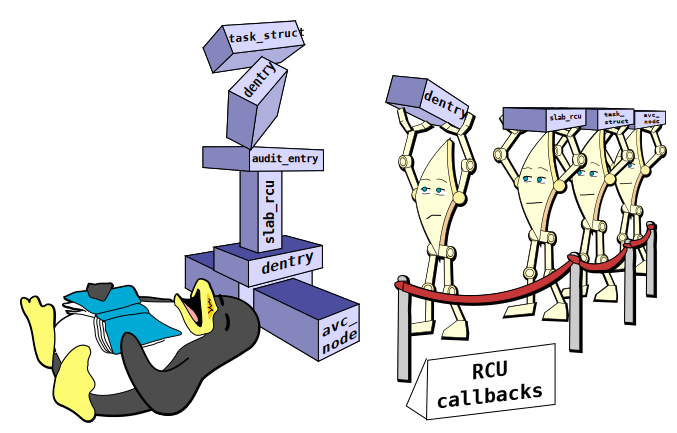
\includegraphics{cartoons/r-2014-RCU-callbacks}}
\caption{Sleeping While RCU Reading Considered Harmful}
\ContributedBy{Figure}{fig:app:rcuimpl:srcu:Sleeping While RCU Reading Considered Harmful}{Melissa Broussard}
\end{figure}

Classic RCU 는 read-side 크리티컬 섹션들이 순수한 스핀락들의 크리티컬 섹션들에
의해 지켜지는 것과 똑같은 규칙을 지킬 것을 필요로 합니다: 블락되거나 sleep
상태에 빠지는 어떠한 종류의 것들도 엄격히 금지됩니다.
이는 많은 경우 RCU 의 사용에 문제가 되었고, Paul 은 RCU read-side 크리티컬 섹션
안에서 임의적으로 잠드는 (또는 블록되는) 것을 허용하는 ``sleepable RCU'' (SRCU)
를 위한 요청을 많이 받았습니다.
Paul 은 기존에는 그런 요청들을 모두 작업할 수 없다고 거부했는데, RCU read-side
안에서 임의로 sleep 상태에 빠지는 것은 grace period 를 불명확하게 연장시킬 수
있는데, 이는 임의의 커다란 양의 메모리가 하나의 grace period 의 종료를 기다리는
결과를 초래할 것이고, 이는 결국
Figure~\ref{fig:app:rcuimpl:srcu:Sleeping While RCU Reading Considered Harmful}
에 그려진 것처럼 대부분의 경우 메모리 부족으로 인한 시스템 멎음 상태의 재앙이
되어버릴 수 있을 것이기 때문이었습니다.
무엇보다도, 시스템 멎음 상태를 초래할 수 있는---심지어 올바르게
사용되었음에도---모든 동시성 제어 기능은 존재할 가치가 없습니다.
\iffalse

Classic RCU requires that read-side critical sections
obey the same rules
obeyed by the critical sections of pure spinlocks: blocking or sleeping
of any sort is strictly prohibited.
This has frequently been an obstacle to the use of RCU, and
Paul has received numerous requests for a ``sleepable RCU'' (SRCU) that
permits arbitrary sleeping (or blocking) within RCU read-side critical
sections.
Paul had previously rejected all such requests as unworkable, since arbitrary
sleeping in RCU read-side could indefinitely extend grace periods, which
in turn could result in arbitrarily large amounts of memory awaiting the
end of a grace period, which finally would result in disaster,
as fancifully depicted in
Figure~\ref{fig:app:rcuimpl:srcu:Sleeping While RCU Reading Considered Harmful},
with the most likely disaster being hangs due to memory exhaustion.
After all, any concurrency-control primitive that could result in
system hangs---even when used correctly---does not deserve to exist.
\fi

하지만, 스핀락 크리티컬 섹션들이 preemption 될 수 있을 것을 필요로 하는
realtime 커널들~\cite{IngoMolnar05a} 또한 RCU read-side 크리티컬 섹션들이
preemption 될 수 있을 것을 필요로 했습니다~\cite{PaulMcKenney05b}.
Preemptible 크리티컬 섹션들은 데드락이 방지될 수 있도록 하기 위해
lock-acquisition 기능이 블록될 수 있을 것을 필요로 했고, 이는 곧 RCU 의, 그리고
스핀락의 크리티컬 섹션들이 락을 기다리며 블록될 수 있음을 의미하게 됩니다.
하지만, 이 두가지 형태의 sleeping 은 이 잠든 task 들을 짧은 시간 내에 깨우기
위해 사용될 수 있는 priority boosting 과 priority inheritance 라는 특수한
속성을 갖습니다.

하지만, realtime 커널들에서의 RCU 의 사용은 ``RCU read-side 크리티컬 섹션들은
결코 잠들 수 없다'' 라고 새겨져 있는 석판에 생겨난 첫번째 흠집이었습니다.
그렇다고는 하나, 들어오는 TCP 연결을 기다리면서 블록되는 것과 같은 불명확한
시간동안의 잠듦은 realtime 커널들에서조차도 엄격히 금지되어 있습니다.
\iffalse

However, the realtime kernels that require spinlock critical sections
be preemptible~\cite{IngoMolnar05a} also require that RCU read-side critical
sections be preemptible~\cite{PaulMcKenney05b}.
Preemptible critical sections in turn require that lock-acquisition
primitives block in order to avoid deadlock,
which in turns means that both RCU's and spinlocks'
critical sections be able to block awaiting a lock.
However, these two forms of sleeping have the special property that
priority boosting and priority inheritance may be used to awaken
the sleeping tasks in short order.

Nevertheless,
use of RCU in realtime kernels was the first crack in the tablets
of stone on which were inscribed ``RCU read-side critical sections can never
sleep''.
That said, indefinite sleeping, such as blocking waiting for an
incoming TCP connection, is strictly verboten even in realtime kernels.
\fi

\QuickQuiz{}
	Classic RCU read-side 크리티컬 섹션 안에서는 왜 잠드는 행위가 금지되어
	있었나요?
	\iffalse

	Why is sleeping prohibited within Classic RCU read-side
	critical sections?
	\fi
\QuickQuizAnswer{
	잠드는 행위는 Classic RCU 에서는 quiescent state 인 컨텍스트 스위치를
	암시하며, RCU 의 grace-period 탐지는 RCU read-side 크리티컬 섹션
	내에서는 quiescent state 가 결코 나타나지 말아야 할것을 필요로 하기
	때문입니다.
	\iffalse

	Because sleeping implies a context switch, which in Classic RCU is
	a quiescent state, and RCU's grace-period detection requires that
	quiescent states never appear in RCU read-side critical sections.
	\fi
} \QuickQuizEnd

\QuickQuiz{}
	quiescent state 에서 컨텍스트 스위치를 제거해버리고, user-mode 수행과
	idle loop 를 quiescent state 로 남겨둠으로써 Classic RCU read-side
	크리티컬 섹션에서의 잠드는 행위를 허용하는건 어떻습니까?
	\iffalse

	Why not permit sleeping in Classic RCU read-side critical sections
	by eliminating context switch as a quiescent state, leaving user-mode
	execution and idle loop as the remaining quiescent states?
	\fi
\QuickQuizAnswer{
	이는 상당한 kernel-mode 수행으로 이루어진 부하를 갖는 시스템 (e.x: 커널
	쓰레드로 인해) 은 grace period 의 완료를 하지 못해서 금방이든 나중이든
	메모리 부족을 일으킬 겁니다.
	\iffalse

	This would mean that a system undergoing heavy kernel-mode
	execution load (e.g., due to kernel threads) might never
	complete a grace period, which
	would cause it to exhaust memory sooner or later.
	\fi
} \QuickQuizEnd

\subsection{SRCU Implementation Strategy}
\label{sec:app:rcuimpl:SRCU Implementation Strategy}

SRC 를 설계하는데 있어서의 주요한 도전점은 RCU read-side 크리티컬 섹션 내에서
잠드는 task 가 무한히 많은 RCU callback 들을 블록 하는 것을 방지하는 것입니다.
SRCU 는 이 목표를 달성하기 위해 두개의 전략을 사용합니다:
\begin{enumerate}
\item	Classic RCU 의 \co{call_rcu()} API 와 같은 비동기적인 grace-period
	인터페이스를 제공하지 않습니다, 그리고
\item	grace-period 탐지를 각각의 SRCU 를 사용하는 subsystem 내로
	격리시킵니다.
\end{enumerate}
이런 전략들의 근본적 이유는 다음 섹션들에서 다루어집니다.
\iffalse

The primary challenge in designing an SRCU
is to prevent any given task sleeping in an RCU read-side
critical section from blocking an unbounded number of RCU callbacks.
SRCU uses two strategies to achieve this goal:
\begin{enumerate}
\item	refusing to provide asynchronous grace-period interfaces,
	such as the Classic RCU's \co{call_rcu()} API, and
\item	isolating grace-period detection within each subsystem using SRCU.
\end{enumerate}
The rationale for these strategies are discussed in the following sections.
\fi

\subsubsection{Abolish Asynchronous Grace-Period APIs}
\label{sec:app:rcuimpl:Abolish Asynchronous Grace-Period APIs}

\co{call_rcu()} API 에서의 문제는 다음에 표현된 것처럼 하나의 쓰레드가 grace
period 를 기다리는 무한히 큰 수의 메모리 블록들을 만들 수 있다는 겁니다:
\iffalse

The problem with the \co{call_rcu()} API is that a single thread can
generate an arbitrarily large number of blocks of memory awaiting a
grace period, as illustrated by the following:
\fi

\vspace{5pt}
\begin{minipage}[t]{\columnwidth}
\scriptsize
\begin{verbatim}
 1 while (p = kmalloc(sizeof(*p), GFP_ATOMIC))
 2   call_rcu(&p->rcu, f);
\end{verbatim}
\end{minipage}
\vspace{5pt}

반대로, \co{synchronize_rcu()} 를 사용하는 비슷한 코드는 쓰레드당 grace period
를 기다리는 메모리 블록은 단 하나까지만 만들 수 있습니다:
\iffalse

In contrast, the analogous code using \co{synchronize_rcu()} can
have at most a single block of memory per thread awaiting a grace period:
\fi

\vspace{5pt}
\begin{minipage}[t]{\columnwidth}
\scriptsize
\begin{verbatim}
 1 while (p = kmalloc(sizeof(*p),
 2                    GFP_ATOMIC)) {
 3   synchronize_rcu();
 4   kfree(&p->rcu, f);
 5 }
\end{verbatim}
\end{minipage}
\vspace{5pt}

따라서, SRCU 는 \co{synchronize_rcu()} 와 동일한 기능은 제공하지만
\co{call_rcu()} 에 대해서는 동일한 기능을 제공하지 않습니다.
\iffalse

Therefore, SRCU provides an equivalent to \co{synchronize_rcu()}, but not
to \co{call_rcu()}.
\fi

\subsubsection{Isolate Grace-Period Detection}
\label{sec:app:rcuimpl:Isolate Grace-Period Detection}

Classic RCU 에서는 단일 read-side 크리티컬 섹션이 무한하게 \emph{모든} RCU
callback 들을 지연시킬 수 있는데, 예를 들면 다음과 같습니다:
\iffalse

In Classic RCU, a single read-side critical section could indefinitely
delay \emph{all} RCU callbacks, for example, as follows:
\fi

\vspace{5pt}
\begin{minipage}[t]{\columnwidth}
\scriptsize
\begin{verbatim}
 1 /* BUGGY: Do not use!! */
 2 rcu_read_lock();
 3 schedule_timeout_interruptible(longdelay);
 4 rcu_read_unlock();
\end{verbatim}
\end{minipage}
\vspace{5pt}

이런 부류의 동작은 만약 RCU 가 grace period 의 긴 시간동안의 지연에도 돌아갈 수
있도록 주의깊게 설계된 하나의 subsystem 안에서만 사용되었다면 해결될 수도
있었을 겁니다.
이 긴 시간동안의 RCU read-side 지연이 사라지도록 강제한 RCU 의 \emph{모든}
사용자를 하나의 격리된 subsystem 안에서의 하나의 RCU read-side 버그가 지연시킬
수 있다는게 사실입니다.

이 문제를 우회할 수 있는 한가지 방법은 grace-period 탐지가
subsystem-by-subsystem 기반으로 이루어지도록 해서, 혼수상태의 RCU 읽기 쓰레드는
grace period 를 해당 읽기 쓰레드의 subsystem 내에서만 지연시키도록 하는
것입니다.
각각의 subsystem 은 grace period 를 기다리는 메모리 블록들을 제한된 숫자까지만
가질 수 있고, subsystem 의 수 역시 짐작건대 제한되어 있으므로, grace period 를
기다리는 메모리의 양 역시 제한될 겁니다.
특정 subsystem 의 설계자는 반드시: (1) SRCU read-side sleeping 이 제한되어
있음을 분명히 보장하고 (2) \co{synchronize_srcu()} 를 기다리는 메모리의 양을
제한해야만 합니다.\footnote{
	예를 들어, SRCU 로 보호되는 해시 테이블은 hash chain 당 하나의 락을
	가질 수 있어서, hash chain 당 최대 하나의 블록이
	\co{synchronize_srcu()} 를 기다리도록 할 수 있습니다.}

이게 정확히 SRCU 가 취한 방법으로, 다음 섹션에서 설명됩니다.
\iffalse

This sort of behavior might be tolerated if RCU were used only within
a single subsystem that was carefully designed to withstand long-term
delay of grace periods.
It is the fact that a single RCU read-side bug in one isolated subsystem can
delay \emph{all} users of RCU that forced these long-term RCU read-side
delays to be abolished.

One way around this issue is for grace-period detection to be performed
on a subsystem-by-subsystem basis, so that a lethargic RCU reader will
delay grace periods only within that reader's subsystem.
Since each subsystem can have only a bounded number of memory blocks
awaiting a grace period, and since the number of subsystems is also
presumably bounded, the total amount of memory awaiting a grace period
will also be bounded.
The designer of a given subsystem is responsible for: (1) ensuring that
SRCU read-side sleeping is bounded and (2) limiting the amount of memory
waiting for \co{synchronize_srcu()}.\footnote{
	For example, an SRCU-protected hash table might have a lock
	per hash chain, thus allowing at most one block per hash
	chain to be waiting for \co{synchronize_srcu()}.}

This is precisely the approach that SRCU takes, as described in the
following section.
\fi

\subsection{SRCU API and Usage}
\label{sec:app:rcuimpl:SRCU API and Usage}

SRCU API 가 Figure~\ref{fig:app:rcuimpl:SRCU API} 에 보여져 있습니다.
다음 섹션은 이걸 어떻게 사용하는지 설명합니다.
\iffalse

The SRCU API is shown in Figure~\ref{fig:app:rcuimpl:SRCU API}.
The following sections describe how to use it.
\fi

\begin{figure}[htbp]
{ \scriptsize
\begin{verbatim}
int init_srcu_struct(struct srcu_struct *sp);
void cleanup_srcu_struct(struct srcu_struct *sp);
int srcu_read_lock(struct srcu_struct *sp);
void srcu_read_unlock(struct srcu_struct *sp, int idx);
void synchronize_srcu(struct srcu_struct *sp);
long srcu_batches_completed(struct srcu_struct *sp);
\end{verbatim}
}
\caption{SRCU API}
\label{fig:app:rcuimpl:SRCU API}
\end{figure}

\subsubsection{Initialization and Cleanup}
\label{sec:app:rcuimpl:Initialization and Cleanup}

SRCU 를 사용하는 subsystem 각각은 \co{struct} \co{srcu_struct} 를 이 타입의
변수를 선언하는 것으로, 또는, 예를 들면 \co{kamlloc()} 등을 사용해서 동적으로
메모리를 할당하는 것으로 생성해야만 합니다.
일단 이 구조체가 만들어지면, 이 구조체는 \co{init_srcu_struct()} 로 초기화
되어야 하는데, 이 함수는 성공 시에는 0을, (예를 들어, 메모리 부족 같은 이유로
인한) 실패 시에는 에러 코드를 리턴합니다.

만약 \co{struct} \co{srcu_strcut} 가 동적으로 할당되었다면, 메모리에서 해제되기
전에 \co{cleanup_srcu_struct()} 가 반드시 호출되어야 합니다.
비슷하게, \co{struct} \co{srcu_strcut} 가 리눅스 커널 모듈 내에서 선언된
변수라면, \co{cleanup_srcu_struct()} 는 해당 모듈이 언로드 되기 전에
호출되어야만 합니다.
어떤 방식으로든, 호출자는 \co{cleanup_srcu_struct()} 의 호출 전에 모든 SRCU
read-side 크리티컬 섹션이 완료되었음을 (그리고 더이상 시작되지 않을 것을)
보장해야 합니다.
이를 달성하기 위한 방법 중 한가지가
Section~\ref{sec:app:rcuimpl:Cleaning Up Safely} 에서 설명됩니다.
\iffalse

Each subsystem using SRCU must create an
\co{struct} \co{srcu_struct},
either by declaring a variable of this type or by
dynamically allocating the memory, for example, via \co{kmalloc()}.
Once this structure is in place, it must be initialized via
\co{init_srcu_struct()}, which returns zero for success or an error
code for failure (for example, upon memory exhaustion).

If the \co{struct} \co{srcu_struct} is dynamically allocated, then
\co{cleanup_srcu_struct()} must be called before it is freed.
Similarly, if the \co{struct} \co{srcu_struct} is a variable declared within
a Linux kernel module, then \co{cleanup_srcu_struct()} must be called
before the module is unloaded.
Either way, the caller must take care to ensure that all SRCU read-side
critical sections have completed (and that no more will commence) before
calling \co{cleanup_srcu_struct()}.
One way to accomplish this is described in
Section~\ref{sec:app:rcuimpl:Cleaning Up Safely}.
\fi

\subsubsection{Read-Side Primitives}
\label{sec:app:rcuimpl:Read-Side Primitives}

The read-side \co{srcu_read_lock()} and \co{srcu_read_unlock()} primitives
are used as shown:

\vspace{5pt}
\begin{minipage}[t]{\columnwidth}
\scriptsize
\begin{verbatim}
 1 idx = srcu_read_lock(&ss);
 2 /* read-side critical section. */
 3 srcu_read_unlock(&ss, idx);
\end{verbatim}
\end{minipage}
\vspace{5pt}

The \co{ss} variable is the \co{struct} \co{srcu_struct} whose initialization
was described in Section~\ref{sec:app:rcuimpl:Initialization and Cleanup},
and the \co{idx} variable is an integer that in effect tells
\co{srcu_read_unlock()} the grace period during which the corresponding
\co{srcu_read_lock()} started.

This carrying of an index is a departure from the RCU API, which,
when required, stores the equivalent information in the task structure.
However, since a given task could potentially occupy an arbitrarily large
number of nested SRCU read-side critical sections, SRCU cannot
reasonably store this index in the task structure.

\subsubsection{Update-Side Primitives}
\label{sec:app:rcuimpl:Update-Side Primitives}

The \co{synchronize_srcu()} primitives may be used as shown below:

\vspace{5pt}
\begin{minipage}[t]{\columnwidth}
\scriptsize
\begin{verbatim}
 1 list_del_rcu(p);
 2 synchronize_srcu(&ss);
 3 kfree(p);
\end{verbatim}
\end{minipage}
\vspace{5pt}

As one might expect by analogy with Classic RCU, this primitive blocks
until until after the completion of all SRCU read-side critical sections
that started before the \co{synchronize_srcu()} started, as shown
in Table~\ref{tab:app:rcuimpl:SRCU Update and Read-Side Critical Sections}.
Here, CPU~1 need only wait for the completion of CPU~0's SRCU read-side
critical section.
It need not wait for the completion of CPU~2's SRCU read-side critical
section, because CPU~2 did not start this critical section until \emph{after}
CPU~1 began executing \co{synchronize_srcu()}.
Finally, CPU~1's \co{synchronize_srcu()} need not wait for CPU~3's
SRCU read-side critical section, because CPU~3 is using \co{s2} rather
than \co{s1} as its \co{struct} \co{srcu_struct}.
CPU~3's SRCU read-side critical section is thus related to a different
set of grace periods than those of CPUs~0 and 2.

\begin{table*}[htb]
\scriptsize
\centering
\begin{tabular}{r|l|l|l|l}
	& \multicolumn{1}{c|}{CPU 0} &
		\multicolumn{1}{c|}{CPU 1} &
			\multicolumn{1}{c|}{CPU 2} &
				\multicolumn{1}{c}{CPU 3} \\
	\hline
	\hline
	1 & \co{i0 = srcu_read_lock(&s1)} & & &
				\co{i3 = srcu_read_lock(&s2)} \\
	\hline
	2 &	& \co{synchronize_srcu(&s1)} enter & & \\
	\hline
	3 & 	&	& \co{i2 = srcu_read_lock(&s1)} & \\
	\hline
	4 & \co{srcu_read_unlock(&s1, i0)} & & & \\
	\hline
	5 &	& \co{synchronize_srcu(&s1)} exit & & \\
	\hline
	6 & 	&	 & \co{srcu_read_unlock(&s1, i2)} & \\
\end{tabular}
\caption{SRCU Update and Read-Side Critical Sections}
\label{tab:app:rcuimpl:SRCU Update and Read-Side Critical Sections}
\end{table*}

The \co{srcu_batches_completed()} primitive may be used to
monitor the progress of a given \co{struct} \co{srcu_struct}'s
grace periods.
This primitive is used in ``torture tests'' that validate SRCU's operation.

\subsubsection{Cleaning Up Safely}
\label{sec:app:rcuimpl:Cleaning Up Safely}

Cleaning up SRCU safely can be a challenge, but fortunately many
uses need not do so.
For example, uses in operating-system kernels that are initialized at
boot time need not be cleaned up.
However, uses within loadable modules must clean up if the corresponding
module is to be safely unloaded.

In some cases, such as the RCU torture module,
only a small known set of threads are using the
SRCU read-side primitives against a particular \co{struct} \co{srcu_struct}.
In these cases, the module-exit code need only kill that set of threads,
wait for them to exit, and then clean up.

In other cases, for example, for device drivers, any thread in the
system might be using the SRCU read-side primitives.
Although one could apply the method of the previous paragraph, this
ends up being equivalent to a full reboot, which can be unattractive.
Figure~\ref{fig:app:rcuimpl:SRCU Safe Cleanup} shows one way that cleanup
could be accomplished without a reboot.

\begin{figure}[htbp]
{ \scriptsize
\begin{verbatim}
  1 int readside(void)
  2 {
  3   int idx;
  4
  5   rcu_read_lock();
  6   if (nomoresrcu) {
  7     rcu_read_unlock();
  8     return -EINVAL;
  9   }
 10   idx = srcu_read_lock(&ss);
 11   rcu_read_unlock();
 12   /* SRCU read-side critical section. */
 13   srcu_read_unlock(&ss, idx);
 14   return 0;
 15 }
 16
 17 void cleanup(void)
 18 {
 19   nomoresrcu = 1;
 20   synchronize_rcu();
 21   synchronize_srcu(&ss);
 22   cleanup_srcu_struct(&ss);
 23 }
\end{verbatim}
}
\caption{SRCU Safe Cleanup}
\label{fig:app:rcuimpl:SRCU Safe Cleanup}
\end{figure}

The \co{readside()} function overlaps an RCU and an SRCU read-side
critical section, with the former running from lines~5-11 and the
latter running from lines~10-13.
The RCU read-side critical section uses Pure
%
% RCU\IfInBook{ (see Section~\ref{sec:advsync:Pure RCU})}
% 	    {~\cite{PaulEdwardMcKenneyPhD}}
%
RCU~\cite{PaulEdwardMcKenneyPhD}
%
to guard the
value of the \co{nomoresrcu} variable.
If this variable is set, we are cleaning up, and therefore must not enter
the SRCU read-side critical section, so we return \co{-EINVAL} instead.
On the other hand, if we are not yet cleaning up, we proceed into the
SRCU read-side critical section.

The \co{cleanup()} function first sets the \co{nomoresrcu} variable
on line~19, but then must wait for all currently executing RCU read-side
critical sections to complete via the \co{synchronize_rcu()} primitive
on line~20.
Once the \co{cleanup()} function reaches line~21, all calls to
\co{readside()} that could possibly have seen \co{nomorersrcu} equal
to zero must have already reached line~11, and therefore already must
have entered their SRCU read-side critical section.
All future calls to \co{readside()} will exit via line~8, and will thus
refrain from entering the read-side critical section.

Therefore, once \co{cleanup()} completes its call to
\co{synchronize_srcu()} on line~21, all SRCU read-side critical sections
will have completed, and no new ones will be able to start.
It is therefore safe on line~22 to call \co{cleanup_srcu_struct()}
to clean up.

\subsection{Implementation}
\label{sec:app:rcuimpl:Implementation}

This section describes SRCU's data structures, initialization and
cleanup primitives, read-side primitives, and update-side primitives.

\subsubsection{Data Structures}
\label{sec:app:rcuimpl:Data Structures}

SRCU's data structures are shown in
Figure~\ref{fig:app:rcuimpl:SRCU Data Structures},
and are depicted schematically in
Figure~\ref{fig:app:whymb:SRCU Data-Structure Diagram}.
The \co{completed} field is a count of the number of grace periods
since the \co{struct} \co{srcu} was initialized, and as shown in the
diagram, its low-order bit is used to index the
\co{struct} \co{srcu_struct_array}.
The \co{per_cpu_ref} field points to the array, and the
\co{mutex} field is used to permit but one \co{synchronize_srcu()} at
a time to proceed.

\begin{figure}[htbp]
{ \scriptsize
\begin{verbatim}
 1 struct srcu_struct_array {
 2   int c[2];
 3 };
 4 struct srcu_struct {
 5   int completed;
 6   struct srcu_struct_array *per_cpu_ref;
 7   struct mutex mutex;
 8 };
\end{verbatim}
}
\caption{SRCU Data Structures}
\label{fig:app:rcuimpl:SRCU Data Structures}
\end{figure}

\begin{figure}[htb]
\centering
% \resizebox{3in}{!}{\includegraphics{appendix/rcuimpl/srcuds}}
\includegraphics{appendix/rcuimpl/srcuds}
\caption{SRCU Data-Structure Diagram}
\label{fig:app:whymb:SRCU Data-Structure Diagram}
\end{figure}

\subsubsection{Initialization Implementation}
\label{sec:app:rcuimpl:Initialization Implementation}

SRCU's initialization function, \co{init_srcu_struct()}, is shown in
Figure~\ref{fig:app:rcuimpl:SRCU Initialization}.
This function simply initializes the fields in the
\co{struct} \co{srcu_struct}, returning zero if initialization succeeds
or \co{-ENOMEM} otherwise.

\begin{figure}[htbp]
{ \scriptsize
\begin{verbatim}
  1 int init_srcu_struct(struct srcu_struct *sp)
  2 {
  3   sp->completed = 0;
  4   mutex_init(&sp->mutex);
  5   sp->per_cpu_ref =
  6     alloc_percpu(struct srcu_struct_array);
  7   return (sp->per_cpu_ref ? 0 : -ENOMEM);
  8 }
\end{verbatim}
}
\caption{SRCU Initialization}
\label{fig:app:rcuimpl:SRCU Initialization}
\end{figure}

SRCU's cleanup functions are shown in
Figure~\ref{fig:app:rcuimpl:SRCU Cleanup}.
The main cleanup function, \co{cleanup_srcu_struct()} is shown
on lines~19-29 of this figure, however, it immediately invokes
\co{srcu_readers_active()}, shown on lines~13-17 of this figure,
to verify that there are no readers currently using this
\co{struct} \co{srcu_struct}.

The \co{srcu_readers_active()} function simply returns the sum of
\co{srcu_readers_active_idx()} on both possible indexes,
while \co{srcu_readers_active_idx()}, as shown on lines~1-11,
sums up the per-CPU counters corresponding to the specified index,
returning the result.

If the value returned from \co{srcu_readers_active()} is non-zero,
then \co{cleanup_srcu_struct()} issues a warning on line~24 and
simply returns on lines~25 and 26, declining to destroy a
\co{struct} \co{srcu_struct} that is still in use.
Such a warning always indicates a bug, and given that the bug
has been reported, it is better to allow the system to continue
with a modest memory leak than to introduce possible memory corruption.

Otherwise, \co{cleanup_srcu_struct()} frees the array of per-CPU
counters and \co{NULL}s the pointer on lines~27 and 28.

\begin{figure}[htbp]
{ \scriptsize
\begin{verbatim}
  1 int srcu_readers_active_idx(struct srcu_struct *sp,
  2                             int idx)
  3 {
  4   int cpu;
  5   int sum;
  6
  7   sum = 0;
  8   for_each_possible_cpu(cpu)
  9     sum += per_cpu_ptr(sp->per_cpu_ref, cpu)->c[idx];
 10   return sum;
 11 }
 12
 13 int srcu_readers_active(struct srcu_struct *sp)
 14 {
 15   return srcu_readers_active_idx(sp, 0) +
 16          srcu_readers_active_idx(sp, 1);
 17 }
 18
 19 void cleanup_srcu_struct(struct srcu_struct *sp)
 20 {
 21   int sum;
 22
 23   sum = srcu_readers_active(sp);
 24   WARN_ON(sum);
 25   if (sum != 0)
 26     return;
 27   free_percpu(sp->per_cpu_ref);
 28   sp->per_cpu_ref = NULL;
 29 }
\end{verbatim}
}
\caption{SRCU Cleanup}
\label{fig:app:rcuimpl:SRCU Cleanup}
\end{figure}

\subsubsection{Read-Side Implementation}
\label{sec:app:rcuimpl:Read-Side Implementation}

The code implementing \co{srcu_read_lock()} is shown in
Figure~\ref{fig:app:rcuimpl:Read-Side Acquisition}.
This function has been carefully constructed to avoid the
need for memory barriers and atomic instructions.

Lines~5 and 11 disable and re-enable preemption, in order to force
the sequence of code to execute unpreempted on a single CPU.
Line~6 picks up the bottom bit of the grace-period counter, which will
be used to select which rank of per-CPU counters is to be used for this
SRCU read-side critical section.
The \co{barrier()} call on line~7 is a directive to the compiler
that ensures that the index is
fetched but once,\footnote{
	Please note that, despite the name, \co{barrier()}
	has absolutely no effect on the CPU's ability to
	reorder execution of both code and of memory accesses.}
so that the index used on line~9 is the same
one returned on line~12.
Lines~8-9 increment the selected counter for the current CPU.\footnote{
	It is important to note that the \co{smp_processor_id()} primitive
	has long-term meaning only if preemption is disabled.
	In absence of preemption disabling, a potential preemption
	immediately following execution of this primitive could
	cause the subsequent code to execute on some other CPU.}
Line~10 forces subsequent execution to occur \emph{after}
lines~8-9, in order to prevent to misordering of any code
in a non-\co{CONFIG_PREEMPT} build, but only
from the perspective of an intervening interrupt handler.
However, in a \co{CONFIG_PREEMPT} kernel, the required \co{barrier()}
call is embedded in the \co{preempt_enable()} on line~11, so the
\co{srcu_barrier()} is a no-op in that case.
Finally, line~12 returns the index so that it may be passed in to the
corresponding \co{srcu_read_unlock()}.

\begin{figure}[htbp]
{ \scriptsize
\begin{verbatim}
  1 int srcu_read_lock(struct srcu_struct *sp)
  2 {
  3   int idx;
  4
  5   preempt_disable();
  6   idx = sp->completed & 0x1;
  7   barrier();
  8   per_cpu_ptr(sp->per_cpu_ref,
  9               smp_processor_id())->c[idx]++;
 10   srcu_barrier();
 11   preempt_enable();
 12   return idx;
 13 }
\end{verbatim}
}
\caption{SRCU Read-Side Acquisition}
\label{fig:app:rcuimpl:Read-Side Acquisition}
\end{figure}

The code for \co{srcu_read_unlock()} is shown in
Figure~\ref{fig:app:rcuimpl:Read-Side Release}.
Again, lines~3 and 7 disable and re-enable preemption so that the
whole code sequence executes unpreempted on a single CPU.
In \co{CONFIG_PREEMPT} kernels, the \co{preempt_disable()} on line~3
contains a \co{barrier()} primitive, otherwise, the \co{barrier()}
is supplied by line~4.
Again, this directive forces the subsequent code to execute after
the critical section from the perspective of intervening
interrupt handlers.
Lines~5 and 6 decrement the counter for this CPU, but with the same
index as was used by the corresponding \co{srcu_read_lock()}.

\begin{figure}[htbp]
{ \scriptsize
\begin{verbatim}
  1 void srcu_read_unlock(struct srcu_struct *sp, int idx)
  2 {
  3   preempt_disable();
  4   srcu_barrier();
  5   per_cpu_ptr(sp->per_cpu_ref,
  6               smp_processor_id())->c[idx]--;
  7   preempt_enable();
  8 }
\end{verbatim}
}
\caption{SRCU Read-Side Release}
\label{fig:app:rcuimpl:Read-Side Release}
\end{figure}

The key point is that a given CPU's counters
can be observed by other CPUs only in
cooperation with that CPU's interrupt handlers.
These interrupt handlers are responsible for ensuring that any needed
memory barriers are executed prior to observing the counters.

\subsubsection{Update-Side Implementation}
\label{sec:app:rcuimpl:Update-Side Implementation}

The key point behind SRCU is that \co{synchronize_sched()}
blocks until all currently-executing preempt-disabled regions of
code complete.
The \co{synchronize_srcu()} primitive makes heavy use of this effect,
as can be seen in
Figure~\ref{fig:app:rcuimpl:Update-Side Implementation}.

Line~5 takes a snapshot of the grace-period counter.
Line~6 acquires the mutex, and lines~7-10 check to see whether
at least two grace periods have elapsed since the snapshot,
and, if so, releases the lock and returns---in this case, someone
else has done our work for us.
Otherwise, line~11 guarantees that any other CPU that sees the
incremented value of the grace period counter in \co{srcu_read_lock()}
also sees any changes made by this CPU prior to entering
\co{synchronize_srcu()}.
This guarantee is required to make sure that any SRCU read-side
critical sections not blocking the next grace period have seen
any prior changes.

Line~12 fetches the bottom bit of the grace-period counter for later
use as an index into the per-CPU counter arrays, and then line~13
increments the grace-period counter.
Line~14 then waits for any currently-executing \co{srcu_read_lock()}
to complete, so that by the time that we reach line~15, all
extant instances of \co{srcu_read_lock()} will be using the updated
value from \co{sp->completed}.
Therefore, the counters sampled in by \co{srcu_readers_active_idx()}
on line~15 are guaranteed to
be monotonically decreasing, so that once their sum reaches zero, it
is guaranteed to stay there.

However, there are no memory barriers in the \co{srcu_read_unlock()}
primitive, so the CPU is within its rights to reorder the counter
decrement up into the SRCU critical section, so that references to
an SRCU-protected data structure could in effect ``bleed out'' of the
SRCU critical section.
This scenario is addressed by the \co{synchronize_sched()} on line~17,
which blocks until all other CPUs executing in \co{preempt_disable()}
code sequences (such as that in \co{srcu_read_unlock()}) complete these
sequences.
Because completion of a given \co{preempt_disable()} code sequence
is observed from the CPU executing that sequence, completion of the
sequence implies completion of any prior SRCU read-side critical section.
Any required memory barriers are supplied by the code making the
observation.

At this point, it is therefore safe to release the mutex as shown
on line~18 and return to the caller, who can now be assured that
all SRCU read-side critical sections sharing the same
\co{struct} \co{srcu_struct}
will observe any update made prior to the call to \co{synchronize_srcu()}.

\begin{figure}[htbp]
{ \scriptsize
\begin{verbatim}
  1 void synchronize_srcu(struct srcu_struct *sp)
  2 {
  3   int idx;
  4
  5   idx = sp->completed;
  6   mutex_lock(&sp->mutex);
  7   if ((sp->completed - idx) >= 2) {
  8     mutex_unlock(&sp->mutex);
  9     return;
 10   }
 11   synchronize_sched();
 12   idx = sp->completed & 0x1;
 13   sp->completed++;
 14   synchronize_sched();
 15   while (srcu_readers_active_idx(sp, idx))
 16     schedule_timeout_interruptible(1);
 17   synchronize_sched();
 18   mutex_unlock(&sp->mutex);
 19 }
\end{verbatim}
}
\caption{SRCU Update-Side Implementation}
\label{fig:app:rcuimpl:Update-Side Implementation}
\end{figure}

\QuickQuiz{}
	Why is it OK to assume that updates separated by
	\co{synchronize_sched()} will be performed in order?
\QuickQuizAnswer{
	Because this property is required for the \co{synchronize_sched()}
	aspect of RCU to work at all.
	For example, consider a code sequence that removes an object
	from a list, invokes \co{synchronize_sched()}, then frees
	the object.
	If this property did not hold, then that object might appear
	to be freed before it was
	removed from the list, which is precisely the situation that
	\co{synchronize_sched()} is supposed to prevent!
} \QuickQuizEnd

\QuickQuiz{}
	Why must line~17 in \co{synchronize_srcu()}
	(Figure~\ref{fig:app:rcuimpl:Update-Side Implementation})
	precede the release of the mutex on line~18?
	What would have to change to permit these two lines to be
	interchanged?
	Would such a change be worthwhile?
	Why or why not?
\QuickQuizAnswer{
	Suppose that the order was reversed, and that CPU~0
	has just reached line~13 of
	\co{synchronize_srcu()}, while both CPU~1 and CPU~2 start executing
	another \co{synchronize_srcu()} each, and CPU~3 starts executing a
	\co{srcu_read_lock()}.
	Suppose that CPU~1 reaches line~6 of \co{synchronize_srcu()}
	just before CPU~0 increments the counter on line~13.
	Most importantly, suppose that
	CPU~3 executes \co{srcu_read_lock()}
	out of order with the following SRCU read-side critical section,
	so that it acquires a reference to some SRCU-protected data
	structure \emph{before} CPU~0 increments \co{sp->completed}, but
	executes the \co{srcu_read_lock()} \emph{after} CPU~0 does
	this increment.
	
	Then CPU~0 will \emph{not} wait for CPU~3 to complete its
	SRCU read-side critical section before exiting the ``while''
	loop on lines~15-16 and releasing the mutex (remember, the
	CPU could be reordering the code).
	
	Now suppose that CPU~2 acquires the mutex next,
	and again increments \co{sp->completed}.
	This CPU will then have to wait for CPU~3 to exit its SRCU
	read-side critical section before exiting the loop on
	lines~15-16 and releasing the mutex.
	But suppose that CPU~3 again executes out of order,
	completing the \co{srcu_read_unlock()} prior to
	executing a final reference to the pointer it obtained
	when entering the SRCU read-side critical section.

	CPU~1 will then acquire the mutex, but see that the
	\co{sp->completed} counter has incremented twice, and
	therefore take the early exit.
	The caller might well free up the element that CPU~3 is
	still referencing (due to CPU~3's out-of-order execution).

	To prevent this perhaps improbable, but entirely possible,
	scenario, the final \co{synchronize_sched()} must precede
	the mutex release in \co{synchronize_srcu()}.

	Another approach would be to change to comparison on
	line~7 of \co{synchronize_srcu()} to check for at
	least three increments of the counter.
	However, such a change would increase the latency of a
	``bulk update'' scenario, where a hash table is being updated
	or unloaded using multiple threads.
	In the current code, the latency of the resulting concurrent
	\co{synchronize_srcu()} calls would take at most two SRCU
	grace periods, while with this change, three would be required.

	More experience will be required to determine which approach
	is really better.
	For one thing, there must first be some use of SRCU with
	multiple concurrent updaters.
} \QuickQuizEnd

\subsection{SRCU Summary}
\label{sec:app:rcuimpl:SRCU Summary}

SRCU provides an RCU-like set of primitives that permit general
sleeping in the SRCU read-side critical sections.
However, it is important to note that SRCU has been used only in
prototype code, though it has passed the RCU torture test.
It will be very interesting to see what use, if any, SRCU sees
in the future.

% \input{appendix/rcuimpl/rcuclassic.tex}  @@@ from Ph.D. dissertation.
% appendix/rcuimpl/rcutree.tex

\section{Hierarchical RCU Overview}
\label{app:rcuimpl:rcutree:Hierarchical RCU Overview}
\OriginallyPublished{Appendix}{app:rcuimpl:rcutree:Hierarchical RCU Overview}{Hierarchical RCU Overview}{Linux Weekly News}{PaulEMcKenney2008HierarchicalRCU}

Classic RCU 의 read-side 기능들은 훌륭한 성능과 확장성을 갖긴 합니다만, 언제
이전부터 존재한 read-side 크리티컬 섹션들이 완료되었는지를 결정하는데 사용되는
update-side 기능들은 수십개의 CPU 들만을 고려한 채 설계되었습니다.
이것들의 확장성은 각 grace period 마다 최소 한번은 각 CPU 에 의해 획득되어야
하는 global lock 에 의해 제한됩니다.
Classic RCU 는 실제로는 수백개의 CPU 들까지도 확장성을 갖고, 대략 천개의 CPU
들까지도 확장성을 갖도록 (더 길어지는 grace period 를 대가로) 꼼수를 부릴 수
있지만, 발전되는 중인 멀티코어 시스템들은 더 높은 확장성을 필요로 할겁니다.
\iffalse

Although Classic RCU's read-side primitives enjoy excellent
performance and scalability, the update-side primitives, which
determine when pre-existing read-side critical sections have
finished, were designed with only a few tens of CPUs in mind.
Their scalability is limited by a global lock that must be
acquired by each CPU at least once during each grace period.
Although Classic RCU actually scales to a couple of hundred CPUs, and
can be tweaked to scale to roughly a thousand CPUs (but at the expense of
extending grace periods), emerging multicore systems will require
it to scale better.
\fi

또한, Classic RCU 는 최적화 되지 않은 dynticks 인터페이스를 가지고 있어서,
Classic RCU 는 매 grace period 마다 최소 한번씩은 깨어나게 할겁니다.
이 문제를 자세히 보려면, 4개의 CPU 만이 바쁘게 유지되고 있을 정도로 적은
부하만을 가지고 있는 16-CPU 시스템을 생각해 보세요.
완벽한 세계에서는, 나머지 열두개의 CPU 들은 에너지를 아끼기 위해 깊은 sleep
모드로 빠져있을 수 있을 겁니다.
불행히도, 네개의 바쁜 CPU 들이 자주 RCU update 동작을 수행한다면, 이 열두개의
idle CPU 들은 자주 깨어나서 상당한 전력을 소모할 겁니다.
따라서, Classic RCU 에의 주요 변경 사항들은 항상 잠들어있는 CPU 들을 놔두어야
합니다.
\iffalse

In addition, Classic RCU has a sub-optimal dynticks interface,
with the result that Classic RCU will wake up every CPU at least
once per grace period.
To see the problem with this, consider a 16-CPU system that
is sufficiently lightly loaded that it is keeping only four
CPUs busy.
In a perfect world, the remaining twelve CPUs could be put into
deep sleep mode in order to conserve energy.
Unfortunately, if the four busy CPUs are frequently performing
RCU updates, those twelve idle CPUs will be awakened frequently,
wasting significant energy.
Thus, any major change to Classic RCU should also leave sleeping CPUs lie.
\fi

Classic 과 hierarchical 구현들 둘 다 Classic RCU 의 semantic 과 동일한 API 들을
가지고 있습니다만, 기존의 구현은 ``classic RCU'' 로 불리울 것이고, 새로운
구현은 ``hierarchical RCU'' 라 불릴 겁니다.
\iffalse

Both the classic and the hierarchical implementations
have Classic RCU semantics and identical APIs, however,
the old implementation will be called ``classic RCU''
and the new implementation will be called ``hierarchical RCU''.
\fi

Section~\ref{app:rcuimpl:rcutree:Review of RCU Fundamentals}
은 RCU 의 기본에 대한 짧은 개괄을 제공하고
Section~\ref{app:rcuimpl:rcutree:Brief Overview of Classic RCU Implementation}
은 기존의 ``Classic RCU'' 구현에 대한 전반적인 개괄을 제공합니다.
Section~\ref{app:rcuimpl:rcutree:RCU Desiderata}
은 RCU 에서 일어나지 않을 것 같은 일들을 나열해보고,
Section~\ref{app:rcuimpl:rcutree:Towards a More Scalable RCU Implementation}
과~\ref{app:rcuimpl:rcutree:Towards a Greener RCU Implementation}
에서는 확장성과 전력 효율성을 위한 설계상의 고려할 점들을 각각 알아보고,
Section~\ref{app:rcuimpl:rcutree:State Machine}
에서 hierarchical RCU state machine 을 설명합니다.
Section~\ref{app:rcuimpl:rcutree:Use Cases},
Section~\ref{app:rcuimpl:rcutree:Testing}
는 테스트를 다루고, 마지막으로
Section~\ref{app:rcuimpl:rcutree:Conclusion}
에서 결론을 내립니다.
\iffalse

Section~\ref{app:rcuimpl:rcutree:Review of RCU Fundamentals}
gives a brief review of RCU fundamentals and
Section~\ref{app:rcuimpl:rcutree:Brief Overview of Classic RCU Implementation}
gives a brief overview of the old ``Classic RCU'' implementation.
Section~\ref{app:rcuimpl:rcutree:RCU Desiderata}
lists RCU desiderata,
Sections~\ref{app:rcuimpl:rcutree:Towards a More Scalable RCU Implementation}
and~\ref{app:rcuimpl:rcutree:Towards a Greener RCU Implementation}
lay out design considerations for scalability and energy efficiency,
respectively, and
Section~\ref{app:rcuimpl:rcutree:State Machine}
describes the hierarchical RCU state machine.
Section~\ref{app:rcuimpl:rcutree:Use Cases},
Section~\ref{app:rcuimpl:rcutree:Testing}
covers testing, and finally,
Section~\ref{app:rcuimpl:rcutree:Conclusion}
presents concluding remarks.
\fi

\subsection{Review of RCU Fundamentals}
\label{app:rcuimpl:rcutree:Review of RCU Fundamentals}

가장 기본적 형태에 있어, RCU 는 일이 끝나길 기다리는 방법입니다.
물론, 일이 끝나길 기다리는 방법은 레퍼런스 카운트, reader-writer 락, 이벤트,
등등 매우 많이 존재합니다.
RCU 의 커다란 장점은 (대략) 20,000 개의 서로 다른 일들을 명시적으로 하나하나 다
정보를 추적할 필요 없이, 그리고 명시적 추적에서는 피할 수 없는 성능의 하락,
확장성의 제약, 복잡한 데드락 시나리오, 메모리 누수 문제 없이 각각 기다릴 수
있다는 겁니다.
\iffalse

In its most basic form, RCU is a way of waiting for things to finish.
Of course, there are a great many other ways of waiting for things to
finish, including reference counts, reader-writer locks, events, and so on.
The great advantage of RCU is that it can wait for each of
(say) 20,000 different things without having to explicitly
track each and every one of them, and without having to worry about
the performance degradation, scalability limitations, complex deadlock
scenarios, and memory-leak hazards that are inherent in schemes
using explicit tracking.
\fi

RCU 의 경우, 기다리는 것들은 ``RCU read-side 크리티컬 섹션'' 이라 불리웁니다.
하나의 RCU read-side 크리티컬 섹션은 \co{rcu_read_lock()} 기능으로 시작하고,
연관된 \co{rcu_read_unlock()} 기능으로 종료됩니다.
RCU read-side 크리티컬 섹션들은 중첩될 수 있고, 명시적으로 블록되거나 잠들지
않는다면, 상당히 많은 양의 임의적 코드를 포함할 수 있습니다 (
Section~\ref{app:rcuimpl:Sleepable RCU Implementation} 에서 설명한 SRCU 라
불리는 특수한 형태의 RCU 는 SRCU read-side 크리티컬 섹션 내에서의 일반적인
sleeping 을 허용하긴 하지만요).
여러분이 이러한 표준을 준수한다면, 여러분은 \emph{모든} 코드 조각에 대해
완료되길 기다리는데에 RCU 를 사용할 수 있습니다.

RCU 는 언제 이것들이 끝나는지를 간접적으로 판단함으로써 이 기능을 구현하는데,
classic RCU 의 경우 다른 곳~\cite{McKenney98} 에서, preemptible RCU 의 경우
Section~\ref{app:rcuimpl:Preemptible RCU} 에서 자세히 설명합니다.
\iffalse

In RCU's case, the things waited on are called
``RCU read-side critical sections''.
An RCU read-side critical section starts with an
\co{rcu_read_lock()} primitive, and ends with a corresponding
\co{rcu_read_unlock()} primitive.
RCU read-side critical sections can be nested, and may contain pretty
much any code, as long as that code does not explicitly block or sleep
(although a special form of RCU called SRCU, described in
Section~\ref{app:rcuimpl:Sleepable RCU Implementation}
does permit general sleeping in SRCU read-side critical sections).
If you abide by these conventions, you can use RCU to wait for \emph{any}
desired piece of code to complete.

RCU accomplishes this feat by indirectly determining when these
other things have finished, as has been described
elsewhere~\cite{McKenney98}
for classic RCU and
Section~\ref{app:rcuimpl:Preemptible RCU} for preemptible RCU.
\fi

자세히 말하자면,
page~\pageref{fig:defer:Readers and RCU Grace Period} 의
Figure~\ref{fig:defer:Readers and RCU Grace Period} 에서 보인 바와 같이, RCU 는
앞서 존재하기 시작한 RCU read-side 크리티컬 섹션들과 그것들에 의해 수행된
메모리 오퍼레이션들이 완전히 종료되기를 기다리는 방법입니다.

하지만, 특정 grace period 가 시작한 후에 시작된 RCU read-side 크리티컬 섹션들은
해당 grace period 종료 뒤까지도 연장될 수 있음을 알아두시기 바랍니다.

다음 섹션은 Classic RCU 구현이 어떻게 동작하는지에 대한 높은 수준에서의 개관을
제공합니다.
\iffalse

In particular, as shown in the
Figure~\ref{fig:defer:Readers and RCU Grace Period} on
page~\pageref{fig:defer:Readers and RCU Grace Period},
RCU is a way of
waiting for pre-existing RCU read-side critical sections to completely
finish, also including the memory operations executed
by those critical sections.

However, note that RCU read-side critical sections
that begin after the beginning
of a given grace period can and will extend beyond the end of that grace
period.

The following section gives a very high-level view of how
the Classic RCU implementation operates.
\fi

\subsection{Brief Overview of Classic RCU Implementation}
\label{app:rcuimpl:rcutree:Brief Overview of Classic RCU Implementation}

Classic RCU 구현 아래의 핵심 컨셉은, Classic RCU read-side 크리티컬 섹션은 커널
코드에 국한되어 있고 블록이 허용되어있지 않다는 것입니다.
이말은 언제든 어떤 CPU 가 블록되어 있는 중으로 보이거나, idle loop 을 돌고
있거나, 커널 모드를 빠져나가 있다면, 우리는 해당 CPU 에서 앞서 수행중이던 RCU
read-side 크리티컬 섹션이 모두 완료되었어야 함을 알 수 있다는 것입니다.
그런 상태는 ``quiescent states'' 라 불리며, 각각의 CPU 가 적어도 하나의
quiscent state 를 거쳤다면, 해당 RCU grace period 는 끝납니다.
\iffalse

The key concept behind the Classic RCU implementation is that
Classic RCU read-side critical sections are confined to kernel
code and are not permitted to block.
This means that any time a given CPU is seen
either blocking, in the idle loop, or exiting the kernel, we know that all
RCU read-side critical sections that were previously running on
that CPU must have completed.
Such states are called ``quiescent states'', and
after each CPU has passed through at least one quiescent state,
the RCU grace period ends.
\fi

\begin{figure}[htb]
\centering
\resizebox{3in}{!}{\includegraphics{appendix/rcuimpl/FlatClassicRCU}}
\caption{Flat Classic RCU State}
\label{fig:app:rcuimpl:rcutree:Flat Classic RCU State}
\end{figure}

Classic RCU 의 가장 중요한 데이터 구조는 \co{rcu_ctrlblk} 구조체로,
Figure~\ref{fig:app:rcuimpl:rcutree:Flat Classic RCU State} 에 보인 것처럼 CPU
당 하나의 bit 을 담고 있는 \co{->cpumask} 필드를 가지고 있습니다.
각각의 CPU 의 bit 은 각각의 grace period 의 시작지점에서 1로 설정되고, 각각의
CPU 는 quiescent state 를 지날 때마다 자신의 bit 의 값을 해제합니다.
여러개의 CPU 들이 각자의 bit 을 동시적으로 값 해제하고자 할 수 있으며 이는
\co{->cpumask} 필드를 오염시킬 수 있기 때문에, 그런 문제를 방지하기 위해
\co{->cpumask} 필드를 보호하는데에 \co{->lock} 스핀락이 사용됩니다.
안타깝게도, 멀티코어 트렌드가 지속된다면 곧 흔한 경우가 될 수백개가 넘는 CPU 가
존재한다면 이 스핀락 또한 상당한 경쟁상태로 성능에 악영향을 줄 수 있습니다.
더 나쁜건, \emph{모든} CPU 들이 각자의 bit 을 값 해제해야 한다는 사실은 CPU
들이 grace period 동안은 잠들지 않아야 함을 말하는데, 이는 Linux 의 전력 소모
감소 능력이 제한됨을 말합니다.

다음 섹션은 새로운 real-time 이 아닌 RCU 구현에서 필요한 것들을 나열합니다.
\iffalse

Classic RCU's most important data structure is the \co{rcu_ctrlblk}
structure, which contains the \co{->cpumask} field, which contains
one bit per CPU, as shown in
Figure~\ref{fig:app:rcuimpl:rcutree:Flat Classic RCU State}.
Each CPU's bit is set to one at the beginning of each grace period,
and each CPU must clear its bit after it passes through a quiescent
state.
Because multiple CPUs might want to clear their bits concurrently,
which would corrupt the \co{->cpumask} field, a
\co{->lock}
spinlock is used to protect \co{->cpumask}, preventing any
such corruption.
Unfortunately, this spinlock can also suffer extreme contention if there
are more than a few hundred CPUs, which might soon become quite common
if multicore trends continue.
Worse yet, the fact that \emph{all} CPUs must clear their own bit means
that CPUs are not permitted to sleep through a grace period, which limits
Linux's ability to conserve power.




The next section lays out what we need from a new non-real-time
RCU implementation.
\fi

\subsection{RCU Desiderata}
\label{app:rcuimpl:rcutree:RCU Desiderata}

Real-time RCU 의 요구사항~\cite{PaulMcKenney05b} 을 나열해 보는게 좋은 시작점이
될겁니다:
\iffalse

The list of real-time RCU desiderata~\cite{PaulMcKenney05b}
is a very good start:
\fi

\begin{enumerate}
\item	하나의 RCU grace period 는 모든 이전부터 존재한 RCU read-side 크리티컬
	섹션들이 완료될 때까지 끝날 수 없도록 하는 지연된 해체.
\item	일년 365일 24시간 지속되는 동작을 지원할 수 있는 신뢰성.
\item	Irq 핸들러에서 호출할 수 있을 것.
\item	너무 많은 콜백들이 존재한다면 grace period 들을 신속히 처리할 수 있는
	메커니즘이 존재할 수 있도록 하는, 억제된 메모리 사용량 (LCA2005
	리스트로 효력이 약화되었습니다.)
\item	RCU 가 어떤 있음직한 메모리 할당자와도 동작할 수 있도록 해주는 메모리
	블락들의 독립성.
\item	CPU 나 태스크의 지역적 메모리 에서의 평범한, 어토믹하지 않은 인스트럭션
	동작이 허용될 수 있도록 하는 동기화에 자유로운 read side (이건 LCA2005
	리스트에서 강화되었습니다.).
\item	Update-side 락이 RCU read-side 크리티컬 섹션 내에서 획득되어지는,
	리눅스 커널의 여러곳에서 사용되는 무조건적인 read-to-write 업그레이드.
\item	호환성 있는 API.
\iffalse

\item	Deferred destruction, so that an RCU grace period cannot end
	until all pre-existing RCU read-side critical sections have
	completed.
\item	Reliable, so that RCU supports 24x7 operation for years at
	a time.
\item	Callable from irq handlers.
\item	Contained memory footprint, so that mechanisms exist to expedite
	grace periods if there are too many callbacks.  (This is weakened
	from the LCA2005 list.)
\item	Independent of memory blocks, so that RCU can work with any
	conceivable memory allocator.
\item	Synchronization-free read side, so that only normal non-atomic
	instructions operating on CPU- or task-local memory are permitted.
	(This is strengthened from the LCA2005 list.)
\item	Unconditional read-to-write upgrade, which is used in several
	places in the Linux kernel where the update-side lock is
	acquired within the RCU read-side critical section.
\item	Compatible API.
\fi

\item	이건 real-time RCU 가 될 것은 아니기에, preemption 가능한 RCU read-side
	크리티컬 섹션에 대한 요구사항은 빠졌습니다.
	하지만, 과거 수년동안의 변경사항들을 처리하기 위해 다음의 새로운
	요구사항들을 추가할 필요가 있습니다.

\item	극단적으로 낮은 internal-to-RCU 락 경쟁상황을 갖는 확장성.
	RCU 는 최소 1,024 개, 가능하면 최소 4,096 개의 CPU 들을 지원해야
	합니다.
\item	전력 효율성: RCU 는 저전력 상태의 dynticks-idle CPU 들을 깨우지
	않으면서도 언제 현재의 grace period 가 종료되는지를 알 수 있어야
	합니다.
	이는 real-time RCU 에서 구현되었습니다만, 상당한 단순화를 필요로
	합니다.
\item	RCU read-side 크리티컬 섹션들은 irq 핸들러는 물론이고 NMI 핸들러
	내에서도 사용이 가능해야 합니다.  Preemptible RCU 의 경우에는 별도로
	구현된 \co{synchronize_sched()} 덕분에 이 필요성이 없었음을 알아두시기
	바랍니다.
\item	RCU 는 반복되는 CPU-hotplug 오퍼레이션들의 상황에서도 잘 동작해야
	합니다.
	이는 classic RCU 와 real-time RCU 에서의 필요사항들을 가져올 뿐입니다.
\item	앞서 등록된 모든 RCU 콜백들이 완료되길 기다릴 수 있어야만 하는데, 이는
	이미 \co{rcu_barrier()} 의 형태로 제공되긴 합니다.
\iffalse

\item	Because this is not to be a real-time RCU, the requirement for
	preemptible RCU read-side critical sections can be dropped.
	However, we need to add the following new requirements to account
	for changes over the past few years.

\item	Scalability with extremely low internal-to-RCU lock contention.
	RCU must support at least 1,024 CPUs gracefully, and preferably
	at least 4,096.
\item	Energy conservation: RCU must be able to avoid awakening
	low-power-state dynticks-idle CPUs, but still determine
	when the current grace period ends.
	This has been implemented in real-time RCU, but needs serious
	simplification.
\item	RCU read-side critical sections must be permitted in NMI
	handlers as well as irq handlers.  Note that preemptible RCU
	was able to avoid this requirement due to a separately
	implemented \co{synchronize_sched()}.
\item	RCU must operate gracefully in face of repeated CPU-hotplug
	operations.
	This is simply carrying forward a requirement met by both
	classic and real-time.
\item	It must be possible to wait for all previously registered
	RCU callbacks to complete, though this is already provided
	in the form of \co{rcu_barrier()}.
\fi
\item	RCU 와 다양한 무한 루프 버그들, 그리고 RCU grace period 가 종료되기를
	막는 하드웨어 상의 문제들을 진단하는데 도움이 될 수 있도록, 응답을
	하는데 실패하는 CPU 들을 파악할 수 있다면 좋습니다.
\item	하나의 RCU grace period 가 마지막 연관된 RCU read-side 크리티컬 섹션이
	완료되는데에 수백 마이크로세컨드 만이 걸릴 수 있도록 하는 RCU grace
	period 의 극단적인 속도 촉진이 가능하면 좋습니다.
	하지만, 그런 동작은 상당한 CPU 오버헤드를 가져올 거라 예상되어지며,
	각각이 RCU grace period 를 기다려야 하는 긴 일련의 오퍼레이션들을
	처리해야 할때 유용할 겁니다.
\iffalse

\item	Detecting CPUs that are failing to respond is desirable,
	to assist diagnosis both of RCU and of various infinite
	loop bugs and hardware failures that can prevent RCU grace
	periods from ending.
\item	Extreme expediting of RCU grace periods is desirable,
	so that an RCU grace period can be forced to complete within
	a few hundred microseconds of the last relevant RCU read-side
	critical second completing.
	However, such an operation would be expected to incur
	severe CPU overhead, and would be primarily useful when
	carrying out a long sequence of operations that each needed
	to wait for an RCU grace period.
\fi
\end{enumerate}

새로운 효구사항들 가운데 가장 압박이 되는건 첫번째 항목인 확장성입니다.
따라서 다음 섹션은 RCU 의 내부 락들의 경쟁 상황을 수십배 줄여주는지 설명합니다.
\iffalse

The most pressing of the new requirements is the first one, scalability.
The next section therefore describes how to make order-of-magnitude reductions
in contention on RCU's internal locks.
\fi

\subsection{Towards a More Scalable RCU Implementation}
\label{app:rcuimpl:rcutree:Towards a More Scalable RCU Implementation}

\begin{figure}[htb]
\centering
\resizebox{3in}{!}{\includegraphics{appendix/rcuimpl/TreeClassicRCU}}
\caption{Hierarchical RCU State}
\label{fig:app:rcuimpl:rcutree:Hierarchical RCU State}
\end{figure}

락 경쟁을 줄여주는 효과적인 방법 가운데 하나는
Figure~\ref{fig:app:rcuimpl:rcutree:Hierarchical RCU State} 에 보인 것처럼
계층을 만드는 것입니다.
여기서, 각각의 네개의 \co{rcu_node} 구조체는 자신의 락을 가지고 있어서, CPU~0
과 1 만이 좌하단의 \co{rcu_node} 의 락을 획득하며, CPU~2 와 3 만이 중하단의
\co{rcu_node} 의 락을 획득하고, CPU~4 와 5 만이 우하단의 \co{rcu_node} 의 락을
획득합니다.
어떤 특정 grace period 동안에도, 아래쪽 \co{rcu_node} 구조체들에 접근하는 CPU
들 가운데 하나만이 위의 \co{rcu_node} 에 접근하게 되어서, 각각의 CPU 짝 들
가운데 마지막 하나만이 연관된 grace period 에 대한 quiescent state 를 기록하게
됩니다.

이는 락 경쟁의 상당한 감소를 초래합니다:
여섯개의 CPU 들이 하나의 락을 위해 매 grace period 마다 경쟁하는 대신, 위쪽
\co{rcu_node} 락에 세개의 CPU 만이 경쟁하고 (50\% 경쟁 감소) 아래쪽
\co{rcu_node} 의 락에 대해서는 각각 두개의 CPU 만이 경쟁을 합니다 (67\% 경쟁
감소).
\iffalse

One effective way to reduce lock contention is to create a hierarchy,
as shown in
Figure~\ref{fig:app:rcuimpl:rcutree:Hierarchical RCU State}.
Here, each of the four \co{rcu_node} structures has its own lock,
so that only CPUs~0 and 1 will acquire the lower left
\co{rcu_node}'s lock, only CPUs~2 and 3 will acquire the
lower middle \co{rcu_node}'s lock, and only CPUs~4 and 5
will acquire the lower right \co{rcu_node}'s lock.
During any given grace period,
only one of the CPUs accessing each of the lower \co{rcu_node}
structures will access the upper \co{rcu_node}, namely, the
last of each pair of CPUs to record a quiescent state for the corresponding
grace period.

This results in a significant reduction in lock contention:
instead of six CPUs contending for a single lock each grace period,
we have only three for the upper \co{rcu_node}'s lock
(a reduction of 50\%) and only
two for each of the lower \co{rcu_node}s' locks (a reduction
of 67\%).
\fi

\begin{figure}[htb]
\centering
\resizebox{3in}{!}{\includegraphics{appendix/rcuimpl/TreeMapping}}
\caption{Mapping {\tt rcu\_node} Hierarchy Into Array}
\label{fig:app:rcuimpl:rcutree:Mapping rcu-node Hierarchy Into Array}
\end{figure}

\co{rcu_node} 구조체들의 트리는 \co{rcu_state} 구조체 안의 선형적 배열로 트리의
루트를 0번 원소로 저장하는 식으로 내장되는데,
Figure~\ref{fig:app:rcuimpl:rcutree:Mapping rcu-node Hierarchy Into Array} 에
여덟개의 CPU 를 갖는 시스템에서 세 단계를 갖는 계층으로 구성했을 때를 보이고
있습니다.
각각의 화살표는 특정 \co{rcu_node} 구조체를 그 부모로 연결시키는데,
\co{rcu_node} 의 \co{->parent}  필드를 나타냅니다.
각각의 \co{rcu_node} 는 자신이 관리하는 CPU 들의 범위를 나타내는데, 루트 노드는
모든 CPU 들을 관리하고, leaf 레벨의 각각의 노드는 한쌍의 CPU 들을 관리합니다.
이 배열은 컴파일 시점에 \co{NR_CPUS} 값에 따라 정적으로 할당됩니다.
\iffalse

The tree of \co{rcu_node} structures is embedded into
a linear array in the \co{rcu_state} structure,
with the root of the tree in element zero, as shown in
Figure~\ref{fig:app:rcuimpl:rcutree:Mapping rcu-node Hierarchy Into Array}
for an eight-CPU
system with a three-level hierarchy.
Each arrow links a given \co{rcu_node} structure to its parent,
representing the \co{rcu_node}'s \co{->parent} field.
Each \co{rcu_node} indicates the range of CPUs covered,
so that the root node covers all of the CPUs, each node in the second
level covers half of the CPUs, and each node in the leaf level covering
a pair of CPUs.
This array is allocated statically at compile time based on the value
of \co{NR_CPUS}.
\fi

\begin{figure}[htbp]
\centering
\resizebox{3in}{!}{\includegraphics{appendix/rcuimpl/TreeClassicRCUGP}}
\caption{Hierarchical RCU Grace Period}
\label{fig:app:rcuimpl:rcutree:Hierarchical RCU Grace Period}
\end{figure}

Figure~\ref{fig:app:rcuimpl:rcutree:Hierarchical RCU Grace Period}
안의 다이어그램들의 시퀀스는 어떻게 grace period 들이 파악되는지를 보입니다.
첫번째 그림에서는 어떤 CPU 도 빨간 네모로 표시되었듯이 quiescent state 에
이르지 못했습니다.
모든 여섯개의 CPU 들이 동시에 RCU 에게 자신이 quiescent state 에 이르렀노라고
이야기하고자 한다고 생각해 봅시다.
각각의 쌍 안의 CPU 들 중 하나만이 연관된 아래쪽 \co{rcu_node} 의 락을 획득할 수
있을 것이고, 따라서 두번째 그림은 그런 운좋은 CPU 들이 0, 3, 그리고 5 라고
초록색 네모로 나타내고 있습니다.
이 운좋은 CPU 들이 일단 마무리 되면, 다른 CPU 들이 락을 획득할 것인데, 세번째
그림으로 보인 바와 같습니다.
이 CPU 들 각각은 자신들이 자신의 그룹 내에서는 마지막에 이르렀음을 보게 되고,
따라서 모든 세개의 CPU 들은 위쪽의 \co{rcu_node} 로 이동하려 시도하게 됩니다.
한번에 하나만이 위쪽 \co{rcu_node} 구조체의 락을 얻을 수 있고, 네번째,
다섯번째, 그리고 여섯번째 그림은 CPU~1, CPU~2, 그리고 CPU~4 가 순서대로 그 락을
잡는다는 가정 하에 상태의 흐름을 보입니다.
마지막 여섯번째 그림은 모든 CPU 들이 quiescent state 를 지난, 그래서 grace
period 가 끝난 경우를 보이고 있습니다.
\iffalse

The sequence of diagrams in
Figure~\ref{fig:app:rcuimpl:rcutree:Hierarchical RCU Grace Period}
shows how grace periods are detected.
In the first figure, no CPU has yet passed through a quiescent state,
as indicated by the red rectangles.
Suppose that all six CPUs simultaneously try to tell RCU that they have
passed through a quiescent state.
Only one of each pair will be able to acquire the lock on the
corresponding lower \co{rcu_node}, and so the second figure
shows the result if the lucky CPUs are numbers 0, 3, and 5, as indicated
by the green rectangles.
Once these lucky CPUs have finished, then the other CPUs will acquire
the lock, as shown in the third figure.
Each of these CPUs will see that they are the last in their group,
and therefore all three will attempt to move to the upper
\co{rcu_node}.
Only one at a time can acquire the upper \co{rcu_node} structure's
lock, and the fourth, fifth, and sixth figures show the sequence of
states assuming that CPU~1, CPU~2, and CPU~4 acquire
the lock in that order.
The sixth and final figure in the group shows that all CPUs have passed
through a quiescent state, so that the grace period has ended.
\fi

\begin{figure}[htb]
\centering
\resizebox{3in}{!}{\includegraphics{appendix/rcuimpl/BigTreeClassicRCU}}
\caption{Hierarchical RCU State 4,096 CPUs}
\label{fig:app:rcuimpl:rcutree:Hierarchical RCU State 4,096 CPUs}
\end{figure}

앞의 예에서, Classic RCU 에서라면 여섯개의 CPU 들이 경쟁하게 될 터인 것을 어떤
하나의 락에 대해서는 세개가 넘는 CPU 들이 경쟁하지 않았습니다.
하지만, 더 많은 수의 CPU 들에서라면 이보다도 극적인 락 경쟁의 감소가
가능합니다.
64 개의 아래쪽 구조체와 64*64=4,096 CPU 들로 구성된,
Figure~\ref{fig:app:rcuimpl:rcutree:Hierarchical RCU State 4,096 CPUs} 에 보인
것과 같은 \co{rcu_node} 구조체들의 계층을 생각해 보세요.

여기서 각각의 아래쪽 \co{rcu_node} 구조체의 락들은 64 개의 CPU 들에 의해
획득되어지는데, 이는 Classic RCU 의 하나의 글로벌 락에 4,096 개의 CPU 들이
경쟁하는 것에 비해 64배의 감소입니다.
비슷하게, 특정 grace period 동안에, 아래쪽 \co{rcu_node} 구조체의 CPU 들 가운데
하나만이 위쪽 \co{rcu_node} 구조체의 락을 잡을 것이므로, 이는 또다시 4,096 개의
CPU 로 구성된 시스템에서 동작하는 Classic RCU 가 겪게 되는 경쟁의 64x
감소입니다.
\iffalse

In the above sequence, there were never more than three CPUs
contending for any one lock, in happy contrast to Classic RCU,
where all six CPUs might contend.
However, even more dramatic reductions in lock contention are
possible with larger numbers of CPUs.
Consider a hierarchy of \co{rcu_node} structures, with
64 lower structures and 64*64=4,096 CPUs, as shown in
Figure~\ref{fig:app:rcuimpl:rcutree:Hierarchical RCU State 4,096 CPUs}.

Here each of the lower \co{rcu_node} structures' locks
are acquired by 64 CPUs, a 64-times reduction from the 4,096 CPUs
that would acquire Classic RCU's single global lock.
Similarly, during a given grace period, only one CPU from each of
the lower \co{rcu_node} structures will acquire the
upper \co{rcu_node} structure's lock, which is again
a 64x reduction from the contention level that would be experienced
by Classic RCU running on a 4,096-CPU system.
\fi

\QuickQuiz{}
	잠깐만요!
	이 새로운 락들을 가지고, 데드락은 어떻게 막나요?
	\iffalse

	Wait a minute!
	With all those new locks, how do you avoid deadlock?
	\fi
\QuickQuizAnswer{
	한번에 한개의 \co{rcu_node} 구조체의 락만을 잡도록 하는 것으로 데드락이
	막아집니다.
	이 알고리즘은 두개의 락을 더 사용하는데, 하나는 grace-period 진척과
	동시에 CPU hotplug 오퍼레이션이 수행되는 것을 막고 (\co{onofflock})
	또하나는 한번에 하나의 CPU 만이 quiescent state 가 빨리 끝나도록
	강제하는데에 사용됩니다 (\co{fqslock}).
	이것들은 락킹 계층에 반하고, 따라서 \co{fqslock} 은 \co{onofflock} 보다
	먼저 획득되어야만 하는데, 이말은 \co{rcu_node} 구조체의 락들보다 먼저
	획득되어야만 한다는 말입니다.

	또한, 실제 사용에서의 효율이 중요하듯이, 한버에 하나의 \co{rcu_node} 의
	락만을 잡는 것을 거부함은 어떤 것이 잡혀있는지를 추적할 필요가 없음을
	의미합니다.
	그런 추적은 불필요할 뿐 아니라 고통스러울 겁니다.
	\iffalse

	Deadlock is avoided by never holding more than one of the
	\co{rcu_node} structures' locks at a given time.
	This algorithm uses two more locks, one to prevent CPU hotplug
	operations from running concurrently with grace-period advancement
	(\co{onofflock}) and another
	to permit only one CPU at a time from forcing a quiescent state
	to end quickly (\co{fqslock}).
	These are subject to a locking hierarchy, so that
	\co{fqslock} must be acquired before
	\co{onofflock}, which in turn must be acquired before
	any of the \co{rcu_node} structures' locks.

	Also, as a practical matter, refusing to ever hold more than
	one of the \co{rcu_node} locks means that it is unnecessary
	to track which ones are held.
	Such tracking would be painful as well as unnecessary.
	\fi
} \QuickQuizEnd

\QuickQuiz{}
	왜 64-배 감소에서 멈추는 거죠?
	왜 그이상 가서 수백배까지 줄이지 않는거예요?
	\iffalse

	Why stop at a 64-times reduction?
	Why not go for a few orders of magnitude instead?
	\fi
\QuickQuizAnswer{
	RCU 는 수백개의 CPU 을 갖는 시스템에서도 문제없이 동작하기 때문에,
	64개의 CPU 들이 하나의 락을 경쟁하도록 하는 것으로도 충분합니다.
	이 락들은 상당히 드물게 획득되어지므로, 각각의 CPU 는 grace period 마다
	한번씩 정도만 이 일을 하게 될 것이고, grace period 는 밀리세컨드
	단위까지 길어짐을 기억해 두시기 바랍니다.
	\iffalse

	RCU works with no problems on
	systems with a few hundred CPUs, so allowing 64 CPUs to contend on
	a single lock leaves plenty of headroom.
	Keep in mind that these locks are acquired quite rarely, as each
	CPU will check in about one time per grace period, and grace periods
	extend for milliseconds.
	\fi
} \QuickQuizEnd

\QuickQuiz{}
	하지만 전 McKenney 의 Quick Quiz 2 에의 게으른 변명 따위 신경쓰지
	않아요!!!
	저는 하나의 락에 경쟁하는 CPU 들의 수를 16이나 그정도 쯤까지 더
	합리적인 수준으로 낮추고 싶어요!!!
	\iffalse

	But I don't care about McKenney's lame excuses in the answer to
	Quick Quiz 2!!!
	I want to get the number of CPUs contending on a single lock down
	to something reasonable, like sixteen or so!!!
	\fi
\QuickQuizAnswer{
	좋아요, 그럼 그렇게 해보세요!
	\co{CONFIG_RCU_FANOUT=16} 으로 설정하고 (\co{NR_CPUS=4096 에 대해})
	나면 가장 낮은 단계에서의 256 \co{rcu_node} 구조체, 중간 계층에서의 16
	개의 \co{rcu_node} 구조체, 그리고 하나의 root 레벨 \co{rcu_node} 를
	갖게 되어 세단계의 계층을 갖게 될 겁니다.
	이에 대해 지불하게 될 비용은 더 많은 \co{rcu_node} 구조체들이 어떤 CPU
	들이 자신의 quiescent state 를 완료하는데 도움이 필요한지를 체크하는데
	더 많은 작업이 걸릴 거라는 겁니다 (64 대신 256 이 되는거죠).
	\iffalse

	OK, have it your way, then!
	Set \co{CONFIG_RCU_FANOUT=16} and (for \co{NR_CPUS=4096})
	you will get a
	three-level hierarchy with with 256 \co{rcu_node} structures
	at the lowest level, 16 \co{rcu_node} structures as intermediate
	nodes, and a single root-level \co{rcu_node}.
	The penalty you will pay is that more \co{rcu_node} structures
	will need to be scanned when checking to see which CPUs need help
	completing their quiescent states (256 instead of only 64).
	\fi
} \QuickQuizEnd

\begin{figure}[htb]
\centering
\resizebox{3in}{!}{\includegraphics{appendix/rcuimpl/BigTreeClassicRCUBH}}
\caption{Hierarchical RCU State With BH}
\label{fig:app:rcuimpl:rcutree:Hierarchical RCU State With BH}
\end{figure}

실제 구현은 RCU 콜백의 리스트와 같은 per-CPU 데이터를 유지하도록 되어 있으며,
이는 \co{rcu_data} 구조체에 정리되어 있습니다.
또한, rcu (\co{call_rcu()} 에서의) 와 rcu\_bh (\co{call_rcu_bh()} 에서의) 는
각각
Figure~\ref{fig:app:rcuimpl:rcutree:Hierarchical RCU State With BH} 에 보인
것과 같이 각각의 계층을 유지합니다.
\iffalse

The implementation maintains some per-CPU data, such as lists of
RCU callbacks, organized into \co{rcu_data} structures.
In addition, rcu (as in \co{call_rcu()}) and
rcu\_bh (as in \co{call_rcu_bh()}) each maintain their own
hierarchy, as shown in
Figure~\ref{fig:app:rcuimpl:rcutree:Hierarchical RCU State With BH}.
\fi

\QuickQuiz{}
	좋아요, 근데 색깔은 뭘 의미하나요?
	\iffalse

	OK, so what is the story with the colors?
	\fi
\QuickQuizAnswer{
	(\co{rcu_ctrlblk} 을 포함해서) \co{rcu_state} 에 비슷한 데이터 구조들은
	노란색으로, 어떤 CPU 들이 들어와 있는지를 파악하는데 사용되는 bitmap
	들을 포함한 것들은 핑크로, 그리고 per-CPU \co{rcu_data} 구조체들은
	파란색으로 표시되어 있습니다.
	(\co{rcu_dynticks} 와 같이) 전력을 아끼기 위해 사용되는 데이터
	구조체들은 초록색으로 칠해져 있습니다.
	\iffalse

	Data structures analogous to \co{rcu_state} (including
	\co{rcu_ctrlblk}) are yellow,
	those containing the bitmaps used to determine when CPUs have checked
	in are pink,
	and the per-CPU \co{rcu_data} structures are blue.
	The data structures used to conserve energy
	(such as \co{rcu_dynticks}) will be colored green.
	\fi
} \QuickQuizEnd

다음 섹션은 에너지 소모 감소에 대해 이야기 해봅니다.
\iffalse

The next section discusses energy conservation.
\fi

\subsection{Towards a Greener RCU Implementation}
\label{app:rcuimpl:rcutree:Towards a Greener RCU Implementation}

앞서 언급되었듯이, 이러한 노력의 중요한 목표는 전력 소모를 방지하기 위해 잠자는
CPU 들을 깨우지 않는 것입니다.
반면에, Classic RCU 는 잠들어 있는 CPU 들을 어떤 겨웅에 있어서는 매 grace
period 마다 한번씩은 깨울 것인데, 이는 적은 수의 CPU 들만이 바쁘게 일을 하면서
RCU update 를 하고 있고 나머지 대부분의 CPU 들은 idle 상태일 때에
비효율적입니다.
이 상황은 peak load 를 위해 맞춰진 시스템들에서 자주 발생하며, 우린 이런 상황을
잘 대처할 필요가 있습니다.
더 나아가서, 우린 긴시간 동작하는 RCU read-side 크리티컬 섹션을 담고 있으며
인터럽트를 처리하는 dynticks-idle CPU 가 RCU grace period 가 끝나는 것을 막는데
실패하는, Classic RCU 의 오랫동안 있어왔던 버그를 고칠 필요가 있습니다.
\iffalse

As noted earlier, an important goal of this effort is to leave sleeping
CPUs lie in order to promote energy conservation.
In contrast, classic RCU will happily awaken each and every sleeping CPU
at least once per grace period in some cases,
which is suboptimal in the case where
a small number of CPUs are busy doing RCU updates and the majority of
the CPUs are mostly idle.
This situation occurs frequently in systems sized for peak loads, and
we need to be able to accommodate it gracefully.
Furthermore, we need to fix a long-standing bug in Classic RCU where
a dynticks-idle CPU servicing an interrupt containing a long-running
RCU read-side critical section will fail to prevent an RCU grace period
from ending.
\fi

\QuickQuiz{}
	그런 어처구니 없는 버그가 있다면, Linux 는 대체 어떻게 동작하고
	있는거죠?
	\iffalse

	Given such an egregious bug, why does Linux run at all?
	\fi
\QuickQuizAnswer{
	리눅스 커널은 (상대적으로) 얌전한 디바이스 드라이버들을 가지고 있기
	때문입니다.
	만약 그것들 가운데 일부가 RCU read-side 크리티컬 섹션 내에서 spin 을 수
	밀리세컨드까지 한다면 이는 이 버그를 일으킬 수 있습니다.
	그러나 이 버그는 고쳐져야만 하고, 이 RCU 변종은 그런 수정을 합니다.
	\iffalse

	Because the Linux kernel contains device drivers that are (relatively)
	well behaved.
	Few if any of them spin in RCU read-side critical sections for the
	many milliseconds that would be required to provoke this bug.
	The bug nevertheless does need to be fixed, and this variant of
	RCU does fix it.
	\fi
} \QuickQuizEnd

\begin{figure}[htb]
\centering
\resizebox{3in}{!}{\includegraphics{appendix/rcuimpl/BigTreeClassicRCUBHdyntick}}
\caption{Hierarchical RCU State With Dynticks}
\label{fig:app:rcuimpl:rcutree:Hierarchical RCU State With Dynticks}
\end{figure}

이는 모든 CPU 들이 per-CPU \co{rcu_dynticks} 구조체 안에 위치한 카운터들을
조정하도록 함으로써 이루어집니다.
간단히 말해서, 이 카운터들은 연관된 CPU 가 dynticks idle 모드에 있을 경우에는
짝수의 값을 가지고, 그렇지 않을 때에는 홀수의 값을 갖습니다.
따라서 RCU 는 이 \co{rcu_dynticks} 카운터들이 홀수인 CPU 들에 대해서만
quiescent state 를 기다리면 되고, 그 카운터의 값이 짝수인 잠들어있는 CPU 들은
깨울 필요가 없습니다.
Figure~\ref{fig:app:rcuimpl:rcutree:Hierarchical RCU State With Dynticks} 에
보여진 것처럼, 각각의 per-CPU \co{rcu_dynticks} 구조체는 ``rcu'' 와 ``rcu\_bh''
구현에 의해 공유됩니다.

다음 섹션은 높은 레벨에서의 RCU state machine 에 대한 개요를 보입니다.
\iffalse

This is accomplished by requiring that all CPUs manipulate counters
located in a per-CPU \co{rcu_dynticks} structure.
Loosely speaking, these counters have even-numbered values when the
corresponding CPU is in dynticks idle mode, and have odd-numbered values
otherwise.
RCU thus needs to wait for quiescent states only for those CPUs whose
\co{rcu_dynticks} counters are odd, and need not wake up sleeping
CPUs, whose counters will be even.
As shown in
Figure~\ref{fig:app:rcuimpl:rcutree:Hierarchical RCU State With Dynticks},
each per-CPU \co{rcu_dynticks} structure
is shared by the ``rcu'' and ``rcu\_bh'' implementations.

The following section presents a high-level view of the RCU state machine.
\fi

\subsection{State Machine}
\label{app:rcuimpl:rcutree:State Machine}

\begin{figure}[htbp]
\centering
\resizebox{3in}{!}{\includegraphics{appendix/rcuimpl/GenericRCUStateMachine}}
\caption{Generic RCU State Machine}
\label{fig:app:rcuimpl:rcutree:Generic RCU State Machine}
\end{figure}

충분히 높은 단계에서 보면, 리눅스 커널 RCU 구현은
Figure~\ref{fig:app:rcuimpl:rcutree:Generic RCU State Machine} 에 보인 state
machine 으로 볼 수 있습니다.
바쁘게 동작하는 시스템에서의 이 state machine 의 일반적인 경우의 수행경로는
가장 위쪽 두개의 루프로ㅡ 각각의 grace period (GP) 의 시작으로 초기화되어서,
quiescent state (QS) 를 기다리고, 각 CPU 가 grace period 동안 첫번째 quiescent
state 를 지나가는 경로입니다.
그런 시스템에서는, quiescent state 는 각 컨텍스트 스위치마다 발생할 수도 있고,
idle 이거나 user-mode 코드를 수행중인 CPU 에서는 각 scheduling-clock 인터럽트
마다 발생할 수 있습니다.
CPU-hotplug 이벤트는 state machine 을 ``CPU Offline'' 상자로 가져가게 되며,
quiescent state 로의 빠른 전환을 실패하게 하는 ``holdout'' CPU 들의 존재 시에는
``Send resched IPIs to Hodout CPUs'' 상자로의 전환을 일으킬 겁니다.
불필요하게 dyntick-idle CPU 들을 불필요하게 깨우는 것을 막는 RCU 구현은 그런
CPU 들을 연장된 quiescent state 에 있는 것으로 표시해 둘 것이고 ``CPUs in
dyntick-idle Mode?'' 결정 마름모꼴의 ``Y'' 브랜치를 취하게 될 것입니다 (하지만
dyntick-idle 모드의 CPU 들은 resched IPI 들을 보내지 \emph{않을} 것임을
알아두세요).
마지막으로, \co{CONFIG_RCU_CPU_STALL_DETECTOR} 가 켜져있다면, quiescent state
에 이르기까지의 정말로 너무 긴 딜레이는 ``Complain About Holdout CPUs'' 경로를
수행하게 만들겁니다.
\iffalse

At a sufficiently high level, Linux-kernel RCU implementations can
be thought of as high-level state machines as shown in
Figure~\ref{fig:app:rcuimpl:rcutree:Generic RCU State Machine}.
The common-case path through this state machine on a busy system
goes through the two uppermost loops, initializing at the
beginning of each grace period (GP),
waiting for quiescent states (QS), and noting when each CPU passes through
its first quiescent state for a given grace period.
On such a system, quiescent states will occur on each context switch,
or, for CPUs that are either idle or executing user-mode code, each
scheduling-clock interrupt.
CPU-hotplug events will take the state machine through the
``CPU Offline'' box, while the presence of ``holdout''
CPUs that fail to pass through quiescent states quickly enough will exercise
the path through the ``Send resched IPIs to Holdout CPUs'' box.
RCU implementations that avoid unnecessarily awakening dyntick-idle
CPUs will mark those CPUs as being in an extended quiescent state,
taking the ``Y'' branch out of the ``CPUs in dyntick-idle
Mode?'' decision diamond (but note that CPUs in dyntick-idle mode
will \emph{not} be sent resched IPIs).
Finally, if \co{CONFIG_RCU_CPU_STALL_DETECTOR} is enabled,
truly excessive delays in reaching quiescent states will exercise the
``Complain About Holdout CPUs'' path.
\fi

\QuickQuiz{}
	하지만 이 state diagram 은 dyntick-idle CPU 들이 reschedule IPI 들을
	맞게 될 것을 보이고 있지 않나요?  그게 그것들을 깨워버리지 않을까요?
	\iffalse

	But doesn't this state diagram indicate that dyntick-idle CPUs will
	get hit with reschedule IPIs?  Won't that wake them up?
	\fi
\QuickQuizAnswer{
	아니요.
	RCU 는 CPU 그룹들을 처리하고 있음을 명심하세요.
	하나의 특정한 그룹은 dyntick-idle CPU 들과 어떻게든 quiescent state 를
	지나는 것을 막도록 관리되는 평범한 모드의 CPU 들을 모두 포함하고 있을
	수 있습니다.
	뒤쪽 그룹들만이 reschedule IPI 를 받을 겁니다; dyntick-idle CPU 들은
	단지 extended quiescent state 로 표시되어질 뿐입니다.
	\iffalse

	No.
	Keep in mind that RCU is handling groups of CPUs.
	One particular group might contain both dyntick-idle CPUs and
	CPUs in normal mode that have somehow managed to avoid passing through
	a quiescent state.
	Only the latter group will be sent a reschedule IPI; the dyntick-idle
	CPUs will merely be marked as being in an extended quiescent state.
	\fi
} \QuickQuizEnd

\begin{figure}[htb]
\centering
\resizebox{3in}{!}{\includegraphics{appendix/rcuimpl/TreeRCUStateMachine}}
\caption{RCU State Machine and Hierarchical RCU Data Structures}
\label{fig:app:rcuimpl:rcutree:RCU State Machine and Hierarchical RCU Data Structures}
\end{figure}

앞의 satte machine 의 내용은 또다른 데이터 구조와 상호작용하게 되는데,
Figure~\ref{fig:app:rcuimpl:rcutree:RCU State Machine and Hierarchical RCU Data Structures}
에 보인 것과 같습니다.
하지만, 이 state machine 의 내용은 어떤 RCU 구현에 있어서도 그대로 C 코드로
변환되어지지는 않습니다.
그보다는, 이 구현들은 커널 내에 event-driven 코드로 만들어져 있습니다.
따라서, 다음 섹션은 일부 ``사용 예'', 또는 RCU 알고리즘이 앞의 state machine 의
내용을 진행하는 방법은 물론이고 관련된 데이터 구조를 알아봅니다.
\iffalse

The events in the above state schematic interact with different
data structures, as shown in
Figure~\ref{fig:app:rcuimpl:rcutree:RCU State Machine and Hierarchical RCU Data Structures}.
However, the state schematic does not directly translate into C code
for any of the RCU implementations.
Instead, these implementations are coded as an event-driven system within
the kernel.
Therefore, the following section describes some ``use cases'',
or ways in which the RCU algorithm traverses the above state schematic
as well as the relevant data structures.
\fi

\subsection{Use Cases}
\label{app:rcuimpl:rcutree:Use Cases}

이 섹션은 사용되는 데이터 구조들과 호출되는 함수들을 나열하며 RCU 구현 내에서의
몇가지 ``사용 예'' 들에 대한 개요를 제공합니다.
이 사용 예들은 다음과 같습니다:
\iffalse

This section gives an overview of several ``use cases''
within the RCU implementation, listing the data structures touched
and the functions invoked.
The use cases are as follows:
\fi

\begin{enumerate}
\item	새로운 Grace Period 의 시작
	(Section~\ref{app:rcuimpl:rcutree:Start a New Grace Period})
\item	Quiescent State 의 통과
	(Section~\ref{app:rcuimpl:rcutree:Pass Through a Quiescent State})
\item	RCU 에게 Quiescent State 를 알리기
	(Section~\ref{app:rcuimpl:rcutree:Announce a Quiescent State to RCU})
\item	Dynticks Idle Mode 의 진입과 빠져나오기
	(Section~\ref{app:rcuimpl:rcutree:Enter and Leave Dynticks Idle Mode})
\item	Dynticks Idle Mode 로부터의 인터럽트
	(Section~\ref{app:rcuimpl:rcutree:Interrupt from Dynticks Idle Mode})
\item	Dynticks Idle Mode 로부터의 NMI
	(Section~\ref{app:rcuimpl:rcutree:NMI from Dynticks Idle Mode})
\item	CPU 가 Dynticks Idle Mode 에 있음을 알기
	(Section~\ref{app:rcuimpl:rcutree:Note That a CPU is in Dynticks Idle Mode})
\item	CPU 를 끄기
	(Section~\ref{app:rcuimpl:rcutree:Offline a CPU})
\item	CPU 를 켜기
	(Section~\ref{app:rcuimpl:rcutree:Online a CPU})
\item	너무 긴 Grace Period 를 감지하기
	(Section~\ref{app:rcuimpl:rcutree:Detect a Too-Long Grace Period})
\iffalse

\item	Start a New Grace Period
	(Section~\ref{app:rcuimpl:rcutree:Start a New Grace Period})
\item	Pass Through a Quiescent State
	(Section~\ref{app:rcuimpl:rcutree:Pass Through a Quiescent State})
\item	Announce a Quiescent State to RCU
	(Section~\ref{app:rcuimpl:rcutree:Announce a Quiescent State to RCU})
\item	Enter and Leave Dynticks Idle Mode
	(Section~\ref{app:rcuimpl:rcutree:Enter and Leave Dynticks Idle Mode})
\item	Interrupt from Dynticks Idle Mode
	(Section~\ref{app:rcuimpl:rcutree:Interrupt from Dynticks Idle Mode})
\item	NMI from Dynticks Idle Mode
	(Section~\ref{app:rcuimpl:rcutree:NMI from Dynticks Idle Mode})
\item	Note That a CPU is in Dynticks Idle Mode
	(Section~\ref{app:rcuimpl:rcutree:Note That a CPU is in Dynticks Idle Mode})
\item	Offline a CPU
	(Section~\ref{app:rcuimpl:rcutree:Offline a CPU})
\item	Online a CPU
	(Section~\ref{app:rcuimpl:rcutree:Online a CPU})
\item	Detect a Too-Long Grace Period
	(Section~\ref{app:rcuimpl:rcutree:Detect a Too-Long Grace Period})
\fi
\end{enumerate}

이 사용 예들 각각은 다음 섹션들에서 설명됩니다.
\iffalse

Each of these use cases is described in the following sections.
\fi

\subsubsection{Start a New Grace Period}
\label{app:rcuimpl:rcutree:Start a New Grace Period}

\co{rcu_start_gp()} 함수는 새로운 grace period 를 시작합니다.
이 함수는 CPU 가 grace period 를 기다리는 콜백을 가지고 있는 CPU 가 어떤 grace
period 도 진행중이 아니란 것을 알릴 때에 호출됩니다.

\co{rcu_start_gp()} 함수는 새로이 시작된 grace period 를 알리기 위해
\co{rcu_state} 와 \co{rcu_data} 구조체의 상태를 업데이트 하는데, 동시의
CPU-hotplug 오퍼레이션들을 배제하기 위해 \co{->onoff} 락을 잡고 (그리고 irq
들을 불능화 시키고), (이 CPU 를 포함해) 모든 CPU 들은 quiescent state 를
지나야만 함을 알리기 위해 모든 \co{rcu_node} 구조체의 bit 들의 값을 설정하고,
마지막으로 \co{->onoff} 락을 해제합니다.
\iffalse

The \co{rcu_start_gp()} function starts a new grace period.
This function is invoked when a CPU having callbacks waiting for a
grace period notices that no grace period is in progress.

The \co{rcu_start_gp()} function updates state in
the \co{rcu_state} and \co{rcu_data} structures
to note the newly started grace period,
acquires the \co{->onoff} lock (and disables irqs) to exclude
any concurrent CPU-hotplug operations,
sets the
bits in all of the \co{rcu_node} structures to indicate
that all CPUs (including this one) must pass through a quiescent
state,
and finally
releases the \co{->onoff} lock.
\fi

이 bit 값 설정 동작은 두개의 페이즈로 진행됩니다.
먼저, non-leaf \co{rcu_node} 구조체의 bit 들은 어떤 락도 더이상 잡지 않은채
설정되고, 이후엔 각각의 leaf \co{rcu_node} 구조체들의 bit 들이 해당 구조체의
\co{->lock} 을 잡은채 설정되어집니다.
\iffalse

The bit-setting operation is carried out in two phases.
First, the non-leaf \co{rcu_node} structures' bits are set without
holding any additional locks, and then finally each leaf \co{rcu_node}
structure's bits are set in turn while holding that structure's
\co{->lock}.
\fi

\QuickQuiz{}
	하지만 한 CPU 가 bit 값 설정하는 CPU 가 종료되기 전에 (자신의 bit 의
	값을 해제하면서) quiescent state 를 지나감을 이야기 하려 하면 어떻게
	되나요?
	\iffalse

	But what happens if a CPU tries to report going through a quiescent
	state (by clearing its bit) before the bit-setting CPU has finished?
	\fi
\QuickQuizAnswer{
	여기서 고려할 세개의 경우가 존재합니다:
	\iffalse

	There are three cases to consider here:
	\fi

	\begin{enumerate}
	\item	아직 초기화 되지 않은 leaf \co{rcu_node} 구조체에 연관된 CPU 가
		quiescent state 를 보고하려 합니다.
		이 CPU 는 이미 자신의 bit 의 값을 해제했고, 따라서 자신의
		quiescent state 를 보고하는 것을 포기할 겁니다.
		나중의 quiescent state 가 새로운 grace period 를 위해 동작될
		겁니다.
	\item	현재 초기화 중인 leaf \co{rcu_node} 구조체에 연관된 CPU 가
		quiescent state 를 보고하려 합니다.
		이 CPU 는 해당 \co{rcu_node} 구조체의 \co{->lock} 이 잡혀
		있음을 보게 되고, 따라서 그 락이 해제될 때까지 spin 을 하게
		됩니다.
		하지만 일단 이 락이 해제되면, \co{rcu_node} 구조체는 초기화
		되었을 것이므로, 다음 경우로 합쳐집니다.
	\item	이미 초기화 된 leaf \co{rcu_node} 에 연관된 CPU 가 quiescent
		state 를 보고하려 합니다.
		이 CPU 는 자신의 bit 에 값이 설정된 것을 보게 되고, 따라서 이를
		해제하려 합니다.
		만약 이게 해당 leaf node 의 마지막 CPU 라면, 계층의 다음 레벨로
		올라갈 겁니다.
		하지만, 이 CPU 는 시스템에서 quiescent state 를 보고하려는
		마지막 CPU 일 수가 없는데, 초기화를 하는 CPU 는 아직
		검사되어졌을 수가 없기 때문입니다.
	\iffalse

	\item	A CPU corresponding to a non-yet-initialized leaf
		\co{rcu_node} structure tries to report a quiescent state.
		This CPU will see its bit already cleared, so will give up on
		reporting its quiescent state.
		Some later quiescent state will serve for the new grace period.
	\item	A CPU corresponding to a leaf \co{rcu_node} structure that
		is currently being initialized tries to report a quiescent
		state.
		This CPU will see that the \co{rcu_node} structure's
		\co{->lock} is held, so will spin until it is
		released.
		But once the lock is released, the \co{rcu_node}
		structure will have been initialized, reducing to the
		following case.
	\item	A CPU corresponding to a leaf \co{rcu_node} that has
		already been initialized tries to report a quiescent state.
		This CPU will find its bit set, and will therefore clear it.
		If it is the last CPU for that leaf node, it will
		move up to the next level of the hierarchy.
		However, this CPU cannot possibly be the last CPU in the
		system to report a quiescent state, given that the CPU
		doing the initialization cannot yet have checked in.
	\fi
	\end{enumerate}

	따라서, 모든 세개의 경우에 있어서, 잠재적인 경주상황은 모두 올바르게
	해결됩니다.
	\iffalse

	So, in all three cases, the potential race is resolved correctly.
	\fi
} \QuickQuizEnd

\QuickQuiz{}
	Bit 값 설정 CPU 가 종료되기 전에 \emph{모든} CPU 들이 quiescent state
	를 지나감을 보고하려고 해서 새로운 grace period 를 시작도 하기 전에
	종료해 버리면 무슨 일이 일어나나요?
	\iffalse

	And what happens if \emph{all} CPUs try to report going
	through a quiescent
	state before the bit-setting CPU has finished, thus ending the new
	grace period before it starts?
	\fi
\QuickQuizAnswer{
	Bit 의 값을 설정하는 CPU 는 초기화 중에 quiescent state 를 지나갈 수가
	없는데, irq 들을 불능화 시켰기 때문입니다.
	따라서 해당 bit 들은 0이 아닌 값으로 남아있어서, 데이터 구조가 완전히
	초기화 되기 전에 grace period 가 종료되는 것을 막습니다.
	\iffalse

	The bit-setting CPU cannot pass through a
	quiescent state during initialization, as it has irqs disabled.
	Its bits therefore remain non-zero, preventing the grace period from
	ending until the data structure has been fully initialized.
	\fi
} \QuickQuizEnd

\subsubsection{Pass Through a Quiescent State}
\label{app:rcuimpl:rcutree:Pass Through a Quiescent State}

RCU 의 rcu 와 rcu\_bh 향은 서로 다른 quiescent state 집합을 갖습니다.
Quiescent state 는 rcu 에 있어서는 컨텍스트 스위치, idle (dynticks 또는 idle
루프), 그리고 user-mode 수행인 반면, rcu\_bh 에 있어서는 interrupt 가 활성화 된
채의 softirq 바깥 모든 코드입니다.
Rcu 를 위한 quiescent state 는 곧 rcu\_bh 를 위한 quiescent state 이기도 하다는
점을 알아 두시기 바랍니다.
Rcu 를 위한 quiescent state 들은 \co{rcu_qsctr_inc()} 를 호출하는 것으로
기록되고, rcu\_bh 를 위한 quiescent state 들은 \co{rcu_bh_qsctr_inc()} 를
호출함으로써 기록되어집니다.
이 두개의 함수들은 각자의 상태를 현재 CPU 의 \co{rcu_data} 구조체 안에
기록합니다.
\iffalse

The rcu and rcu\_bh flavors of RCU have different sets of quiescent
states.
Quiescent states for rcu are context switch, idle (either dynticks or
the idle loop), and user-mode execution, while quiescent states for
rcu\_bh are any code outside of softirq with interrupts enabled.
Note that an quiescent state for rcu is also a quiescent state
for rcu\_bh.
Quiescent states for rcu are recorded by invoking \co{rcu_qsctr_inc()},
while quiescent states for rcu\_bh are recorded by invoking
\co{rcu_bh_qsctr_inc()}.
These two functions record their state in the current CPU's
\co{rcu_data} structure.
\fi

이 함수들은 스케쥴러에서 호출되어지는데, \co{__do_softirq()} 와
\co{rcu_check_callbacks()} 에서입니다.
뒤의 함수는 scheduling-clock 인터럽트에 의해서 호출되어지며, 이 인터럽트가
\co{rcu_qsctr_inc()} 또는 \co{rcu_bh_qsctr_inc()} 를 호출한 quiescent state
에서 발생한 것인지를 판단하기 위해 상태를 분석합니다.
이 함수는 또한 \co{RCU_SOFTIRQ} 에 의해서도 호출되는데, 나중에 softirq
컨텍스트에서 현재 CPU 에서 \co{rcu_process_callbacks()} 를 호출되게 합니다.
\iffalse

These functions are invoked from the scheduler, from
\co{__do_softirq()}, and from \co{rcu_check_callbacks()}.
This latter function is invoked from the scheduling-clock interrupt,
and analyzes state to determine whether this interrupt occurred within
a quiescent state, invoking \co{rcu_qsctr_inc()} and/or
\co{rcu_bh_qsctr_inc()}, as appropriate.
It also raises \co{RCU_SOFTIRQ}, which results in
\co{rcu_process_callbacks()} being invoked on the current
CPU at some later time from softirq context.
\fi

\subsubsection{Announce a Quiescent State to RCU}
\label{app:rcuimpl:rcutree:Announce a Quiescent State to RCU}

앞에서 언급된 \co{rcu_process_callbacks()} 함수는 몇가지 의무를 가지고
있습니다:
\iffalse

The afore-mentioned \co{rcu_process_callbacks()} function
has several duties:
\fi

\begin{enumerate}
\item	언제 너무 오래 유지된 grace period 를 (\co{force_quiescent_state()}를
	통해) 끝낼지 판단하는 것.
\item	다른 CPU 가 grace period 의 끝을 파악했을 때 (\co{rcu_process_gp_end()}
	를 통해) 적절한 행동을 취하는 것.
	``적절한 행동`` 은 이 CPU 의 콜백들을 수행하고 새로운 grace period 를
	기록하는 것을 포함합니다.
	이 똑같은 함수는 다른 CPU 가 새로운 grace period 를 시작하는 것에 대한
	응답으로 상태를 업데이트 합니다.
\item	현재 CPU 의 quiescent state 들을 (결국은 \co{cpu_quiet()} 를 호출하는
	\co{rcu_check_quiescent_state()} 를 통해) RCU 메커니즘의 핵심에 알리는
	것.
	이는 물론 현재 grace period 의 끝을 표시합니다.
\item	진행중인 grace period 가 없고 이 CPU 가 여전히 grace period 를 기다리고
	있는 RCU 콜백들을 가지고 있다면 (\co{cpu_needs_another_gp()} 와
	\co{rcu_start_gp()} 를 통해) 새로운 grace period 를 시작하는 것.
\item	Grace period 가 끝난 이 CPU 의 콜백들을 (\co{rcu_do_batch()} 를 통해)
	호출하는 것.
\iffalse

\item	Determining when to take measures to end an over-long grace period
	(via \co{force_quiescent_state()}).
\item	Taking appropriate action when some other CPU detected the end of
	a grace period (via \co{rcu_process_gp_end()}).
	``Appropriate action`` includes advancing this CPU's
	callbacks and recording the new grace period.
	This same function updates state in response to some other
	CPU starting a new grace period.
\item	Reporting the current CPU's quiescent states to the core RCU
	mechanism (via \co{rcu_check_quiescent_state()}, which
	in turn invokes \co{cpu_quiet()}).
	This of course might mark the end of the current grace period.
\item	Starting a new grace period if there is no grace period in progress
	and this CPU has RCU callbacks still waiting for a grace period
	(via \co{cpu_needs_another_gp()} and
	\co{rcu_start_gp()}).
\item	Invoking any of this CPU's callbacks whose grace period has ended
	(via \co{rcu_do_batch()}).
\fi
\end{enumerate}

이 동작들은 앞의 grace period 로부터의 quiescent state 를 현재의 grace period
에게 보고한다던가 하는 것과 같은 버그를 막기 위해 매우 조심스럽게 짜여져
동작합니다.
\iffalse

These interactions are carefully orchestrated in order to avoid
buggy behavior such as reporting a quiescent state from the previous
grace period against the current grace period.
\fi

\subsubsection{Enter and Leave Dynticks Idle Mode}
\label{app:rcuimpl:rcutree:Enter and Leave Dynticks Idle Mode}

스케쥴러는 dynticks-idle 모드에 들어가기 위해 \co{rcu_enter_nohz()} 를
호출하고, 거기서 나오기 위해 \co{rcu_exit_nohz()} 를 호출합니다.
\co{rcu_enter_nohz()} 함수는 per-CPU \co{dynticks_nesting} 변수와 per-CPU
\co{dynticks} 변수의 값을 증가시키는데, \co{dynticks} 는 따라서 짝수의 값을
가져야만 합니다.
\co{rcu_exit_nohz()} 함수는 같은 per-CPU \co{dynticks_nesting} 변수의 값을
감소시키고 per-CPU \co{dynticks} 카운터의 값을 증가시키는데, 따라서
\co{dynticks} 는 홀수 값을 갖게 됩니다.

\co{dynticks} 카운터는 다른 CPU 에 의해 보여질 수 있습니다.
만약 그 값이 짝수라면, 첫번째 CPU 는 연장된 quiescent state 안에 있는 것입니다.
비슷하게, 만약 그 카운터의 값이 grace period 동안 바뀌었다면, 첫번째 CPU 는
grace period 동안의 언젠가에 연장된 quiescent state 안에 있었던 셈입니다.
하지만, 또한 보여져야만 하는 \co{dynticks_nmi} per-CPU 변수가 하나 더 있는데,
이에 대해 아래에서 설명합니다.
\iffalse

The scheduler invokes \co{rcu_enter_nohz()} to
enter dynticks-idle mode, and invokes \co{rcu_exit_nohz()}
to exit it.
The \co{rcu_enter_nohz()} function increments a per-CPU
\co{dynticks_nesting} variable and
also a per-CPU \co{dynticks} counter, the latter of which must
then have an even-numbered value.
The \co{rcu_exit_nohz()} function decrements this same
per-CPU \co{dynticks_nesting} variable,
and again increments the per-CPU \co{dynticks}
counter, the latter of which must then have an odd-numbered value.

The \co{dynticks} counter can be sampled by other CPUs.
If the value is even, the first CPU is in an extended quiescent state.
Similarly, if the counter value changes during a given grace period,
the first CPU must have been in an extended quiescent state at some
point during the grace period.
However, there is another \co{dynticks_nmi} per-CPU variable
that must also be sampled, as will be discussed below.
\fi

\subsubsection{Interrupt from Dynticks Idle Mode}
\label{app:rcuimpl:rcutree:Interrupt from Dynticks Idle Mode}

Dynticks idle 모드로부터의 인터럽트는 \co{rcu_irq_enter()} 와
\co{rcu_irq_exit()} 에서 처리되어집니다.
\co{rcu_irq_enter()} 함수는 per-CPU \co{dynticks_nesting} 변수의 값을
증가시키고, 만약 기존 값이 0 이었다면, \co{dynticks} per-CPU 변수의 값 또한
증가시킵니다 (이제 홀수 값을 갖게 될겁니다).

\co{rcu_irq_exit()} 함수는 per-CPU \co{dynticks_nesting} 변수의 값을
감소시키고, 새로운 값이 0이라면, \co{dynticks} per-CPU 변수의 값을 증가시킵니다
(이제 짝수 값을 갖게 될겁니다).

Irq 핸들러에 들어가게 되면 dynticks idle 모드를 빠져나가는 것이고 그 반대도
성립됨을 알아두시기 바랍니다.
이렇게 들어가고 빠져나오는게 서로 일치하지 못하는 것은 상당한 혼란을 가져올 수
있습니다.
경고 드렸습니다.
\iffalse

Interrupts from dynticks idle mode are handled by
\co{rcu_irq_enter()} and \co{rcu_irq_exit()}.
The \co{rcu_irq_enter()} function increments the
per-CPU \co{dynticks_nesting} variable, and, if the prior
value was zero, also increments the \co{dynticks}
per-CPU variable (which must then have an odd-numbered value).

The \co{rcu_irq_exit()} function decrements the
per-CPU \co{dynticks_nesting} variable, and, if the new
value is zero, also increments the \co{dynticks}
per-CPU variable (which must then have an even-numbered value).

Note that entering an irq handler exits dynticks idle mode
and vice versa.
This enter/exit anti-correspondence can cause much confusion.
You have been warned.
\fi

\subsubsection{NMI from Dynticks Idle Mode}
\label{app:rcuimpl:rcutree:NMI from Dynticks Idle Mode}

NMIs from dynticks idle mode are handled by \co{rcu_nmi_enter()}
and \co{rcu_nmi_exit()}.
These functions both increment the \co{dynticks_nmi} counter,
but only if the aforementioned \co{dynticks} counter is even.
In other words, NMI's refrain from manipulating the
\co{dynticks_nmi} counter if the NMI occurred in non-dynticks-idle
mode or within an interrupt handler.

The only difference between these two functions is the error checks,
as \co{rcu_nmi_enter()} must leave the \co{dynticks_nmi}
counter with an odd value, and \co{rcu_nmi_exit()} must leave
this counter with an even value.

\subsubsection{Note That a CPU is in Dynticks Idle Mode}
\label{app:rcuimpl:rcutree:Note That a CPU is in Dynticks Idle Mode}

The \co{force_quiescent_state()} function implements a
three-phase state machine.
The first phase (\co{RCU_INITIALIZING}) waits for \co{rcu_start_gp()}
to complete grace-period initialization.
This state is not exited by \co{force_quiescent_state()}, but rather
by \co{rcu_start_gp()}.

In the second phase (\co{RCU_SAVE_DYNTICK}), the
\co{dyntick_save_progress_counter()} function scans the CPUs that
have not yet reported a quiescent state, recording their per-CPU
\co{dynticks} and \co{dynticks_nmi} counters.
If these counters both have even-numbered values, then the corresponding
CPU is in dynticks-idle state, which is therefore noted as an extended
quiescent state (reported via \co{cpu_quiet_msk()}).

In the third phase (\co{RCU_FORCE_QS}), the
\co{rcu_implicit_dynticks_qs()} function again scans the CPUs
that have not yet reported a quiescent state (either explicitly or
implicitly during the \co{RCU_SAVE_DYNTICK} phase), again checking the
per-CPU \co{dynticks} and \co{dynticks_nmi} counters.
If each of these has either changed in value or is now even, then
the corresponding CPU has either passed through or is now in dynticks
idle, which as before is noted as an extended quiescent state.

If \co{rcu_implicit_dynticks_qs()} finds that a given CPU
has neither been in dynticks idle mode nor reported a quiescent state,
it invokes \co{rcu_implicit_offline_qs()}, which checks to see
if that CPU is offline, which is also reported as an extended quiescent
state.
If the CPU is online, then \co{rcu_implicit_offline_qs()} sends
it a reschedule IPI in an attempt to remind it of its duty to report
a quiescent state to RCU.

Note that \co{force_quiescent_state()} does not directly
invoke either \co{dyntick_save_progress_counter()} or
\co{rcu_implicit_dynticks_qs()}, instead passing these functions
to an intervening \co{rcu_process_dyntick()} function that
abstracts out the common code involved in scanning the CPUs and reporting
extended quiescent states.

\QuickQuiz{}
	And what happens if one CPU comes out of dyntick-idle mode and then
	passed through a quiescent state just as another CPU notices that the
	first CPU was in dyntick-idle mode?
	Couldn't they both attempt to report a quiescent state at the same
	time, resulting in confusion?
\QuickQuizAnswer{
	They will both attempt to acquire the lock on the same leaf
	\co{rcu_node} structure.
	The first one to acquire the lock will report the quiescent state
	and clear the appropriate bit, and the second one to acquire the
	lock will see that this bit has already been cleared.
} \QuickQuizEnd

\QuickQuiz{}
	But what if \emph{all} the CPUs end up in dyntick-idle mode?
	Wouldn't that prevent the current RCU grace period from ever ending?
\QuickQuizAnswer{
	Indeed it will!
	However, CPUs that have RCU callbacks are not permitted to enter
	dyntick-idle mode, so the only way that \emph{all} the CPUs could
	possibly end up in dyntick-idle mode would be if there were
	absolutely no RCU callbacks in the system.
	And if there are no RCU callbacks in the system, then there is no
	need for the RCU grace period to end.
	In fact, there is no need for the RCU grace period to even
	\emph{start}.

	RCU will restart if some irq handler does a \co{call_rcu()},
	which will cause an RCU callback to appear on the corresponding CPU,
	which will force that CPU out of dyntick-idle mode, which will in turn
	permit the current RCU grace period to come to an end.
} \QuickQuizEnd

\QuickQuiz{}
	Given that \co{force_quiescent_state()} is a three-phase state
	machine, don't we have triple the scheduling latency due to scanning
	all the CPUs?
\QuickQuizAnswer{
	Ah, but the three phases will not execute back-to-back on the same CPU,
	and, furthermore, the first (initialization) phase doesn't do any
	scanning.
	Therefore, the scheduling-latency hit of the three-phase algorithm
	is no different than that of a single-phase algorithm.
	If the scheduling latency becomes a problem, one approach would be to
	recode the state machine to scan the CPUs incrementally, most likely
	by keeping state on a per-leaf-\co{rcu_node} basis.
	But first show me a problem in the real world, \emph{then}
	I will consider fixing it!
} \QuickQuizEnd

\subsubsection{Offline a CPU}
\label{app:rcuimpl:rcutree:Offline a CPU}

CPU-offline events cause \co{rcu_cpu_notify()} to invoke
\co{rcu_offline_cpu()}, which in turn invokes
\co{__rcu_offline_cpu()} on both the rcu and the rcu\_bh
instances of the data structures.
This function clears the outgoing CPU's bits so that future grace
periods will not expect this CPU to announce quiescent states,
and further invokes \co{cpu_quiet()} in order to announce
the offline-induced extended quiescent state.
This work is performed with the global \co{->onofflock}
held in order to prevent interference with concurrent grace-period
initialization.

\QuickQuiz{}
	But the other reason to hold \co{->onofflock} is to prevent
	multiple concurrent online/offline operations, right?
\QuickQuizAnswer{
	Actually, no!
	The CPU-hotplug code's synchronization design prevents multiple
	concurrent CPU online/offline operations, so only one CPU
	online/offline operation can be executing at any given time.
	Therefore, the only purpose of \co{->onofflock} is to prevent a CPU
	online or offline operation from running concurrently with grace-period
	initialization.
} \QuickQuizEnd

\subsubsection{Online a CPU}
\label{app:rcuimpl:rcutree:Online a CPU}

CPU-online events cause \co{rcu_cpu_notify()} to invoke
\co{rcu_online_cpu()}, which initializes the incoming CPU's
dynticks state, and then invokes \co{rcu_init_percpu_data()}
to initialize the incoming CPU's \co{rcu_data} structure,
and also to set this CPU's bits (again protected by
the global \co{->onofflock}) so that future grace periods
will wait for a quiescent state from this CPU.
Finally, \co{rcu_online_cpu()}
sets up the RCU softirq vector for this CPU.

\QuickQuiz{}
	Given all these acquisitions of the global \co{->onofflock},
	won't there
	be horrible lock contention when running with thousands of CPUs?
\QuickQuizAnswer{
	Actually, there can be only three acquisitions of this lock per grace
	period, and each grace period lasts many milliseconds.
	One of the acquisitions is by the CPU initializing for the current
	grace period, and the other two onlining and offlining some CPU.
	These latter two cannot run concurrently due to the CPU-hotplug
	locking, so at most two CPUs can be contending for this lock at any
	given time.

	Lock contention on \co{->onofflock} should therefore
	be no problem, even on systems with thousands of CPUs.
} \QuickQuizEnd

\QuickQuiz{}
	Why not simplify the code by merging the detection of dyntick-idle
	CPUs with that of offline CPUs?
\QuickQuizAnswer{
	It might well be that such merging may eventually be the right
	thing to do.
	In the meantime, however, there are some challenges:

	\begin{enumerate}
	\item	CPUs are not allowed to go into dyntick-idle mode while they
		have RCU callbacks pending, but CPUs \emph{are} allowed to go
		offline with callbacks pending.
		This means that CPUs going offline need to have their callbacks
		migrated to some other CPU, thus, we cannot allow CPUs to
		simply go quietly offline.
	\item	Present-day Linux systems run with \co{NR_CPUS}
		much larger than the actual number of CPUs.
		A unified approach could thus end up uselessly waiting on
		CPUs that are not just offline, but which never existed in
		the first place.
	\item	RCU is already operational when CPUs get onlined one
		at a time during boot, and therefore must handle the online
		process.
		This onlining must exclude grace-period initialization, so
		the \co{->onofflock} must still be used.
	\item	CPUs often switch into and out of dyntick-idle mode
		extremely frequently, so it is not reasonable to use the
		heavyweight online/offline code path for entering and exiting
		dyntick-idle mode.
	\end{enumerate}
} \QuickQuizEnd

\subsubsection{Detect a Too-Long Grace Period}
\label{app:rcuimpl:rcutree:Detect a Too-Long Grace Period}

When the \co{CONFIG_RCU_CPU_STALL_DETECTOR} kernel parameter
is specified, the \co{record_gp_stall_check_time()} function
records the time and also a timestamp set three seconds into the future.
If the current grace period still has not ended by that time, the
\co{check_cpu_stall()} function will check for the culprit,
invoking \co{print_cpu_stall()} if the current CPU is the
holdout, or \co{print_other_cpu_stall()} if it is some other CPU.
A two-jiffies offset helps ensure that CPUs report on themselves
when possible, taking advantage of the fact that a CPU can normally
do a better job of tracing its own stack than it can tracing some other
CPU's stack.

\subsection{Testing}
\label{app:rcuimpl:rcutree:Testing}

RCU is fundamental synchronization code, so any failure of RCU
results in random, difficult-to-debug memory corruption.
It is therefore extremely important that RCU be \emph{highly} reliable.
Some of this reliability stems from careful design, but at the
end of the day we must also rely on heavy stress testing, otherwise
known as torture.

Fortunately, although there has been some debate as to exactly
what populations are covered by the provisions of the Geneva Convention
% <a href="http://www.unhchr.ch/html/menu3/b/91.htm">Geneva Convention</a>,
it is still the case that it does not apply to software.
Therefore, it is still legal to torture your software.
In fact, it is strongly encouraged, because if you don't torture your
software, it will end up torturing \emph{you} by crashing at the most
inconvenient times imaginable.

Therefore, we torture RCU quite vigorously using the rcutorture module.

However, it is not sufficient to torture the common-case uses of RCU.
It is also necessary to torture it in unusual situations, for example,
when concurrently onlining and offlining CPUs and when CPUs are concurrently
entering and exiting dynticks idle mode.
I use a simple scripts to online and offline CPUs that runs concurently
with the rcutorture module.
This module is given the \co{test_no_idle_hz} module parameter in order
to stress-test dynticks idle mode.
Just to be fully paranoid, I sometimes run a kernbench workload in parallel
as well.
Ten hours of this sort of torture on a 128-way machine seems sufficient
to shake out most bugs.

Even this is not the complete story.
As Alexey Dobriyan and Nick Piggin demonstrated in early 2008, it is
also necessary to torture RCU with all relevant combinations of kernel
parameters.
The relevant kernel parameters may be identified using yet another
simple script, and are as follows:

\begin{enumerate}
\item    \co{CONFIG_CLASSIC_RCU}: Classic RCU.
\item    \co{CONFIG_PREEMPT_RCU}: Preemptible (real-time) RCU.
\item    \co{CONFIG_TREE_RCU}: Classic RCU for huge SMP systems.
\item    \co{CONFIG_RCU_FANOUT}: Number of children for each
		\co{rcu_node}.
\item    \co{CONFIG_RCU_FANOUT_EXACT}: Balance the
		\co{rcu_node} tree.
\item    \co{CONFIG_HOTPLUG_CPU}: Allow CPUs to be offlined
		and onlined.
\item    \co{CONFIG_NO_HZ}: Enable dyntick-idle mode.
\item    \co{CONFIG_SMP}: Enable multi-CPU operation.
\item    \co{CONFIG_RCU_CPU_STALL_DETECTOR}: Enable RCU to detect
		when CPUs go on extended quiescent-state vacations.
\item    \co{CONFIG_RCU_TRACE}: Generate RCU trace files in debugfs.
\end{enumerate}

We ignore the \co{CONFIG_DEBUG_LOCK_ALLOC} configuration
variable under the perhaps-naive assumption that hierarchical RCU
could not have broken lockdep.
There are still 10 configuration variables, which would result in
1,024 combinations if they were independent boolean variables.
Fortunately the first three are mutually exclusive, which reduces
the number of combinations down to 384, but \co{CONFIG_RCU_FANOUT}
can take on values from 2 to 64, increasing the number of combinations
to 12,096.
This is an infeasible number of combinations.

One key observation is that only \co{CONFIG_NO_HZ}
and \co{CONFIG_PREEMPT} can be expected to have changed behavior
if either \co{CONFIG_CLASSIC_RCU} or
\co{CONFIG_PREEMPT_RCU} are in effect, as only these portions
of the two pre-existing RCU implementations were changed during this effort.
This cuts out almost two thirds of the possible combinations.

Furthermore, not all of the possible values of
\co{CONFIG_RCU_FANOUT} produce significantly different results,
in fact only a few cases really need to be tested separately:

\begin{enumerate}
\item	Single-node ``tree''.
\item	Two-level balanced tree.
\item	Three-level balanced tree.
\item	Autobalanced tree, where \co{CONFIG_RCU_FANOUT}
	specifies an unbalanced tree, but such that it is auto-balanced
	in absence of \co{CONFIG_RCU_FANOUT_EXACT}.
\item	Unbalanced tree.
\end{enumerate}

Looking further, \co{CONFIG_HOTPLUG_CPU} makes sense only
given \co{CONFIG_SMP}, and \co{CONFIG_RCU_CPU_STALL_DETECTOR}
is independent, and really only needs to be tested once (though someone
even more paranoid than am I might decide to test it both with
and without \co{CONFIG_SMP}).
Similarly, \co{CONFIG_RCU_TRACE} need only be tested once,
but the truly paranoid (such as myself) will choose to run it both with
and without \co{CONFIG_NO_HZ}.

This allows us to obtain excellent coverage of RCU with only 15
test cases.
All test cases specify the following configuration parameters in order
to run rcutorture and so that \co{CONFIG_HOTPLUG_CPU=n} actually
takes effect:

\vspace{5pt}
\begin{minipage}[t]{\columnwidth}
\scriptsize
\begin{verbatim}
CONFIG_RCU_TORTURE_TEST=m
CONFIG_MODULE_UNLOAD=y
CONFIG_SUSPEND=n
CONFIG_HIBERNATION=n
\end{verbatim}
\end{minipage}
\vspace{5pt}

The 15 test cases are as follows:

\begin{enumerate}
\item	Force single-node ``tree'' for small systems:

\vspace{5pt}
\begin{minipage}[t]{\columnwidth}
\scriptsize
\begin{verbatim}
	CONFIG_NR_CPUS=8
	CONFIG_RCU_FANOUT=8
	CONFIG_RCU_FANOUT_EXACT=n
	CONFIG_RCU_TRACE=y
	CONFIG_PREEMPT_RCU=n
	CONFIG_CLASSIC_RCU=n
	CONFIG_TREE_RCU=y
\end{verbatim}
\end{minipage}
\vspace{5pt}

\item	Force two-level tree for large systems:

\vspace{5pt}
\begin{minipage}[t]{\columnwidth}
\scriptsize
\begin{verbatim}
	CONFIG_NR_CPUS=8
	CONFIG_RCU_FANOUT=4
	CONFIG_RCU_FANOUT_EXACT=n
	CONFIG_RCU_TRACE=n
	CONFIG_PREEMPT_RCU=n
	CONFIG_CLASSIC_RCU=n
	CONFIG_TREE_RCU=y
\end{verbatim}
\end{minipage}
\vspace{5pt}

\item	Force three-level tree for huge systems:

\vspace{5pt}
\begin{minipage}[t]{\columnwidth}
\scriptsize
\begin{verbatim}
	CONFIG_NR_CPUS=8
	CONFIG_RCU_FANOUT=2
	CONFIG_RCU_FANOUT_EXACT=n
	CONFIG_RCU_TRACE=y
	CONFIG_PREEMPT_RCU=n
	CONFIG_CLASSIC_RCU=n
	CONFIG_TREE_RCU=y
\end{verbatim}
\end{minipage}
\vspace{5pt}

\item	Test autobalancing to a balanced tree:

\vspace{5pt}
\begin{minipage}[t]{\columnwidth}
\scriptsize
\begin{verbatim}
	CONFIG_NR_CPUS=8
	CONFIG_RCU_FANOUT=6
	CONFIG_RCU_FANOUT_EXACT=n
	CONFIG_RCU_TRACE=y
	CONFIG_PREEMPT_RCU=n
	CONFIG_CLASSIC_RCU=n
	CONFIG_TREE_RCU=y
\end{verbatim}
\end{minipage}
\vspace{5pt}

\item	Test unbalanced tree:

\vspace{5pt}
\begin{minipage}[t]{\columnwidth}
\scriptsize
\begin{verbatim}
	CONFIG_NR_CPUS=8
	CONFIG_RCU_FANOUT=6
	CONFIG_RCU_FANOUT_EXACT=y
	CONFIG_RCU_CPU_STALL_DETECTOR=y
	CONFIG_RCU_TRACE=y
	CONFIG_PREEMPT_RCU=n
	CONFIG_CLASSIC_RCU=n
	CONFIG_TREE_RCU=y
\end{verbatim}
\end{minipage}
\vspace{5pt}

\item	Disable CPU-stall detection:

\vspace{5pt}
\begin{minipage}[t]{\columnwidth}
\scriptsize
\begin{verbatim}
	CONFIG_SMP=y
	CONFIG_NO_HZ=y
	CONFIG_RCU_CPU_STALL_DETECTOR=n
	CONFIG_HOTPLUG_CPU=y
	CONFIG_RCU_TRACE=y
	CONFIG_PREEMPT_RCU=n
	CONFIG_CLASSIC_RCU=n
	CONFIG_TREE_RCU=y
\end{verbatim}
\end{minipage}
\vspace{5pt}

\item	Disable CPU-stall detection and dyntick idle mode:

\vspace{5pt}
\begin{minipage}[t]{\columnwidth}
\scriptsize
\begin{verbatim}
	CONFIG_SMP=y
	CONFIG_NO_HZ=n
	CONFIG_RCU_CPU_STALL_DETECTOR=n
	CONFIG_HOTPLUG_CPU=y
	CONFIG_RCU_TRACE=y
	CONFIG_PREEMPT_RCU=n
	CONFIG_CLASSIC_RCU=n
	CONFIG_TREE_RCU=y
\end{verbatim}
\end{minipage}
\vspace{5pt}

\item	Disable CPU-stall detection and CPU hotplug:

\vspace{5pt}
\begin{minipage}[t]{\columnwidth}
\scriptsize
\begin{verbatim}
	CONFIG_SMP=y
	CONFIG_NO_HZ=y
	CONFIG_RCU_CPU_STALL_DETECTOR=n
	CONFIG_HOTPLUG_CPU=n
	CONFIG_RCU_TRACE=y
	CONFIG_PREEMPT_RCU=n
	CONFIG_CLASSIC_RCU=n
	CONFIG_TREE_RCU=y
\end{verbatim}
\end{minipage}
\vspace{5pt}

\item	Disable CPU-stall detection, dyntick idle mode, and CPU hotplug:

\vspace{5pt}
\begin{minipage}[t]{\columnwidth}
\scriptsize
\begin{verbatim}
	CONFIG_SMP=y
	CONFIG_NO_HZ=n
	CONFIG_RCU_CPU_STALL_DETECTOR=n
	CONFIG_HOTPLUG_CPU=n
	CONFIG_RCU_TRACE=y
	CONFIG_PREEMPT_RCU=n
	CONFIG_CLASSIC_RCU=n
	CONFIG_TREE_RCU=y
\end{verbatim}
\end{minipage}
\vspace{5pt}

\item	Disable SMP, CPU-stall detection, dyntick idle mode, and CPU hotplug:

\vspace{5pt}
\begin{minipage}[t]{\columnwidth}
\scriptsize
\begin{verbatim}
	CONFIG_SMP=n
	CONFIG_NO_HZ=n
	CONFIG_RCU_CPU_STALL_DETECTOR=n
	CONFIG_HOTPLUG_CPU=n
	CONFIG_RCU_TRACE=y
	CONFIG_PREEMPT_RCU=n
	CONFIG_CLASSIC_RCU=n
	CONFIG_TREE_RCU=y
\end{verbatim}
\end{minipage}
\vspace{5pt}

	This combination located a number of compiler warnings.

\item	Disable SMP and CPU hotplug:

\vspace{5pt}
\begin{minipage}[t]{\columnwidth}
\scriptsize
\begin{verbatim}
	CONFIG_SMP=n
	CONFIG_NO_HZ=y
	CONFIG_RCU_CPU_STALL_DETECTOR=y
	CONFIG_HOTPLUG_CPU=n
	CONFIG_RCU_TRACE=y
	CONFIG_PREEMPT_RCU=n
	CONFIG_CLASSIC_RCU=n
	CONFIG_TREE_RCU=y
\end{verbatim}
\end{minipage}
\vspace{5pt}

\item	Test Classic RCU with dynticks idle but without preemption:

\vspace{5pt}
\begin{minipage}[t]{\columnwidth}
\scriptsize
\begin{verbatim}
	CONFIG_NO_HZ=y
	CONFIG_PREEMPT=n
	CONFIG_RCU_TRACE=y
	CONFIG_PREEMPT_RCU=n
	CONFIG_CLASSIC_RCU=y
	CONFIG_TREE_RCU=n
\end{verbatim}
\end{minipage}
\vspace{5pt}

\item	Test Classic RCU with preemption but without dynticks idle:

\vspace{5pt}
\begin{minipage}[t]{\columnwidth}
\scriptsize
\begin{verbatim}
	CONFIG_NO_HZ=n
	CONFIG_PREEMPT=y
	CONFIG_RCU_TRACE=y
	CONFIG_PREEMPT_RCU=n
	CONFIG_CLASSIC_RCU=y
	CONFIG_TREE_RCU=n
\end{verbatim}
\end{minipage}
\vspace{5pt}

\item	Test Preemptible RCU with dynticks idle:

\vspace{5pt}
\begin{minipage}[t]{\columnwidth}
\scriptsize
\begin{verbatim}
	CONFIG_NO_HZ=y
	CONFIG_PREEMPT=y
	CONFIG_RCU_TRACE=y
	CONFIG_PREEMPT_RCU=y
	CONFIG_CLASSIC_RCU=n
	CONFIG_TREE_RCU=n
\end{verbatim}
\end{minipage}
\vspace{5pt}
\item	Test Preemptible RCU without dynticks idle:

\vspace{5pt}

\begin{minipage}[t]{\columnwidth}
\scriptsize
\begin{verbatim}
	CONFIG_NO_HZ=n
	CONFIG_PREEMPT=y
	CONFIG_RCU_TRACE=y
	CONFIG_PREEMPT_RCU=y
	CONFIG_CLASSIC_RCU=n
	CONFIG_TREE_RCU=n
\end{verbatim}
\end{minipage}
\vspace{5pt}
\end{enumerate}

For a large change that affects RCU core code, one should run
rcutorture for each of the above combinations, and concurrently
with CPU offlining and onlining for cases with
\co{CONFIG_HOTPLUG_CPU}.
For small changes, it may suffice to run kernbench in each case.
Of course, if the change is confined to a particular subset of
the configuration parameters, it may be possible to reduce the
number of test cases.

Torturing software: the Geneva Convention does not (yet) prohibit
it, and I strongly recommend it!

\subsection{Conclusion}
\label{app:rcuimpl:rcutree:Conclusion}

This hierarchical implementation of RCU reduces lock contention,
avoids unnecessarily awakening dyntick-idle sleeping CPUs, while
helping to debug Linux's hotplug-CPU code paths.
This implementation is designed to handle single systems with
thousands of CPUs, and on 64-bit systems has an architectural
limitation of a quarter million CPUs, a limit I expect to be
sufficient for at least the next few years.

This RCU implementation of course has some limitations:

\begin{enumerate}
\item	The \co{force_quiescent_state()} can scan the full
	set of CPUs with irqs disabled.
	This would be fatal in a real-time implementation of RCU,
	so if hierarchy ever needs to be introduced to preemptible
	RCU, some other approach will be required.
	It is possible that it will be problematic on 4,096-CPU
	systems, but actual testing on such systems is required
	to prove this one way or the other.
	
	On busy systems, the \co{force_quiescent_state()} scan
	would not be expected to happen,
	as CPUs should pass through quiescent states within three
	jiffies of the start of a quiescent state.  On semi-busy
	systems, only the CPUs in dynticks-idle mode throughout would
	need to be scanned.
	In some cases, for example when a dynticks-idle CPU is handling
	an interrupt during a scan, subsequent scans are required.
	However, each such scan is performed separately, so scheduling
	latency is degraded by the overhead of only one such scan.
	
	If this scan proves problematic, one straightforward solution
	would be to do the scan incrementally.
	This would increase code complexity slightly and would also
	increase the time required to end a grace period, but would
	nonetheless be a likely solution.
	
\item	The \co{rcu_node} hierarchy is created at compile
	time, and is therefore sized for the worst-case \co{NR_CPUS}
	number of CPUs.
	However, even for 4,096 CPUs, the \co{rcu_node}
	hierarchy consumes only 65 cache lines on a 64-bit machine
	(and just you try accommodating 4,096 CPUs on a 32-bit machine!).
	Of course, a kernel built with \co{NR_CPUS=4096}
	running on a 16-CPU machine would use a two-level tree when
	a single-node tree would work just fine.
	Although this configuration would incur added locking overhead,
	this does not affect hot-path read-side code, so should not be a
	problem in practice.
	
\item	This patch does increase kernel text and data somewhat:
	the old Classic RCU implementation consumes 1,757 bytes of
	kernel text and 456 bytes of kernel data for a total of 2,213 bytes,
	while the new hierarchical RCU implementation consumes 4,006
	bytes of kernel text and 624 bytes of kernel data for a total
	of 4,630 bytes on a \co{NR_CPUS=4} system.
	This is a non-problem even for most embedded systems, which
	often come with hundreds of megabytes of main memory.
	However, if this is a problem for tiny embedded systems, it may
	be necessary to provide both ``scale up'' and
	``scale down'' implementations of RCU.
\end{enumerate}

This hierarchical RCU implementation should nevertheless be a vast
improvement over Classic RCU for machines with hundreds of CPUs.
After all, Classic RCU was designed for systems with only 16-32 CPUs.

At some point, it may be necessary to also apply hierarchy to the
preemptible RCU implementation.
This will be challenging due to the modular arithmetic used on the
per-CPU counter pairs, but should be doable.

% appendix/rcuimpl/rcutreewt.tex

\section{Hierarchical RCU Code Walkthrough}
\label{app:rcuimpl:rcutreewt:Hierarchical RCU Code Walkthrough}

이 섹션은 리눅스 커널 hierarchical RCU 코드의 일부 부분들을 분석합니다.
이 섹션은 hierarchical RCU 를 매우 낮은 단계에서 이해하기를 바라는 hard-core
해커들을 위해 지어졌으며, 그런 해커들이라면 먼저
Section~\ref{app:rcuimpl:rcutree:Hierarchical RCU Overview} 를 읽어야 합니다.
하드코어 매저키스트들 역시 이 섹션을 읽어볼 흥미가 생길겁니다.
물론 \emph{진짜} 하드코어 매저키스트들은
Section~\ref{app:rcuimpl:rcutree:Hierarchical RCU Overview} 를 읽기 전에 이
섹션을 읽을 겁니다.
\iffalse

This section walks through selected sections of the Linux-kernel
hierarchical RCU code.
As such, this section is intended for hard-core hackers who wish
to understand hierarchical RCU at a very low level, and such hackers
should first read
Section~\ref{app:rcuimpl:rcutree:Hierarchical RCU Overview}.
Hard-core masochists might also be interested in reading this section.
Of course \emph{really} hard-core masochists will read this section
before reading
Section~\ref{app:rcuimpl:rcutree:Hierarchical RCU Overview}.
\fi

Section~\ref{app:rcuimpl:rcutreewt:Data Structures and Kernel Parameters}
은 데이터 구조와 커널 패러미터들을 설명하고,
Section~\ref{app:rcuimpl:rcutreewt:External Interfaces}
은 외부로의 함수 인터페이스를 다루며,
Section~\ref{app:rcuimpl:rcutreewt:Initialization}
는 초기화 프로세스를 서술하고,
Section~\ref{app:rcuimpl:rcutreewt:CPU Hotplug}
는 CPU-hotplug 인터페이스를 설명하고,
Section~\ref{app:rcuimpl:rcutreewt:Miscellaneous Functions}
는 그외의 유틸리티 함수들을 다루고,
Section~\ref{app:rcuimpl:rcutreewt:Grace-Period-Detection Functions}
는 grace-period 탐지 메커니즘을 설명하고,
Section~\ref{app:rcuimpl:rcutreewt:Dyntick-Idle Functions}
는 dynticks-idle 인터페이스를 보고,
Section~\ref{app:rcuimpl:rcutreewt:Forcing Quiescent States}
는 (offline 과 dynticks-idle CPU 들을 포함해) holdout CPU 들을 다루는 함수들을
알아보고,
Section~\ref{app:rcuimpl:rcutreewt:CPU-Stall Detection}
는 stall 된 CPU, 즉 커널 모드에서 수초 동안을 spinning 하는 CPU 들을 알리는
함수를 보입니다.
마지막으로,
Section~\ref{app:rcuimpl:rcutreewt:Possible Flaws and Changes}
는 있을법한 설계상의 흠결과 수정사항들을 이야기합니다.
\iffalse

Section~\ref{app:rcuimpl:rcutreewt:Data Structures and Kernel Parameters}
describes data structures and kernel parameters,
Section~\ref{app:rcuimpl:rcutreewt:External Interfaces}
covers external function interfaces,
Section~\ref{app:rcuimpl:rcutreewt:Initialization}
presents the initialization process,
Section~\ref{app:rcuimpl:rcutreewt:CPU Hotplug}
explains the CPU-hotplug interface,
Section~\ref{app:rcuimpl:rcutreewt:Miscellaneous Functions}
covers miscellaneous utility functions,
Section~\ref{app:rcuimpl:rcutreewt:Grace-Period-Detection Functions}
describes the mechanics of grace-period detection,
Section~\ref{app:rcuimpl:rcutreewt:Dyntick-Idle Functions}
presents the dynticks-idle interface,
Section~\ref{app:rcuimpl:rcutreewt:Forcing Quiescent States}
covers the functions that handle holdout CPUs (including offline and
dynticks-idle CPUs), and
Section~\ref{app:rcuimpl:rcutreewt:CPU-Stall Detection}
presents functions that report on stalled CPUs, namely those spinning
in kernel mode for many seconds.
Finally,
Section~\ref{app:rcuimpl:rcutreewt:Possible Flaws and Changes}
reports on possible design flaws and fixes.
\fi

\subsection{Data Structures and Kernel Parameters}
\label{app:rcuimpl:rcutreewt:Data Structures and Kernel Parameters}

Hierarchical RCU 데이터 구조의 완전한 이해는 이 알고리즘의 이해에 매우
중요합니다.
따라서,
Section~\ref{app:rcuimpl:rcutreewt:Tracking Dyntick State}
은 각 CPU 의 dyntick-idle state 를 추적하는데 사용되는 데이터 구조들을
설명하고,
Section~\ref{app:rcuimpl:rcutreewt:Nodes in the Hierarchy}
는 \co{rcu_node} 계층을 만드는데 사용되는 per-node 데이터 구조의 필드들을
설명하며,
Section~\ref{app:rcuimpl:rcutreewt:Per-CPU Data}
은 per-CPU \co{rcu_data} 구조체를 설명하고,
Section~\ref{app:rcuimpl:rcutreewt:RCU Global State}
에서는 global \co{rcu_state} 구조체의 필드를 설명하며
Section~\ref{app:rcuimpl:rcutreewt:Kernel Parameters}
에서는 Hierarchical RCU 의 동작을 조절하는 커널 패러미터들을 설명합니다.
\iffalse

A full understanding of the Hierarchical RCU data structures is
critically important to understanding the algorithms.
To this end,
Section~\ref{app:rcuimpl:rcutreewt:Tracking Dyntick State}
describes the data structures used to track each CPU's dyntick-idle state,
Section~\ref{app:rcuimpl:rcutreewt:Nodes in the Hierarchy}
describes the fields in the per-node data structure making up the
\co{rcu_node} hierarchy,
Section~\ref{app:rcuimpl:rcutreewt:Per-CPU Data}
describes per-CPU \co{rcu_data} structure,
Section~\ref{app:rcuimpl:rcutreewt:RCU Global State}
describes the field in the global \co{rcu_state} structure,
and
Section~\ref{app:rcuimpl:rcutreewt:Kernel Parameters}
describes the kernel parameters that control Hierarchical RCU's
operation.
\fi

Page~\pageref{fig:app:rcuimpl:rcutree:Hierarchical RCU State With Dynticks}
의
Figure~\ref{fig:app:rcuimpl:rcutree:Hierarchical RCU State With Dynticks}
와
Page~\pageref{fig:app:rcuimpl:rcutree:Initialized RCU Data Layout}
의
Figure~\ref{fig:app:rcuimpl:rcutree:Initialized RCU Data Layout}
가 다음의 데이터 구조 설명들을 따라가는데에 많은 도움이 될 수 있습니다.
\iffalse

Figure~\ref{fig:app:rcuimpl:rcutree:Hierarchical RCU State With Dynticks}
on
Page~\pageref{fig:app:rcuimpl:rcutree:Hierarchical RCU State With Dynticks}
and
Figure~\ref{fig:app:rcuimpl:rcutree:Initialized RCU Data Layout}
on
Page~\pageref{fig:app:rcuimpl:rcutree:Initialized RCU Data Layout}
can be very helpful in keeping one's place through the following detailed
data-structure descriptions.
\fi

\subsubsection{Tracking Dyntick State}
\label{app:rcuimpl:rcutreewt:Tracking Dyntick State}

Per-CPU \co{rcu_dynticks} 구조체는 다음 필드들을 이용해 dynticks state 를
추적합니다:
\iffalse

The per-CPU \co{rcu_dynticks} structure tracks dynticks state using the
following fields:
\fi

\begin{itemize}
\item	\co{dynticks_nesting}:
	이 \co{int} 는 연관된 CPU 가 RCU read-side 크리티컬 섹션들을 모니터
	되어야 하는 이유의 수를 셉니다.
	만약 이 CPU 가 dynticks-idle 모드에 있다면, 이 필드는 irq 가 감싸진
	횟수를 세고, 그렇지 않다면 irq 감싸진 횟수보다 하나 큰 값을 갖습니다.
\item	\co{dynticks}:
	이 \co{int} 카운터의 값은 연관된 CPU 가 dynticks-idle 모드에 있고 현재
	해당 CPU 에서 수행 중인 irq 핸들러가 없다면 짝수의 값을 갖고, 그렇지
	않다면 홀수의 값을 갖습니다.
	달리 말하자면, 이 카운터의 값이 홀수라면, 연관된 CPU 는 RCU read-side
	크리티컬 섹션에 있을 수 있습니다.
\item	\co{dynticks_nmi}:
	이 \co{int} 카운터의 값은 연관된 CPU 가 NMI 핸들러 수행중이라면
	홀수인데, 이 CPU 가 irq 핸들러 수행중이지 않은 채로 dyntick-idle 모드에
	있는 동안 NMI 를 받았을 때에만 입니다.
	그렇지 않다면, 이 카운터의 값은 짝수입니다.
\iffalse

\item	\co{dynticks_nesting}:
	This \co{int} counts the number of reasons that the corresponding
	CPU should be monitored for RCU read-side critical sections.
	If the CPU is in dynticks-idle mode, then this counts the
	irq nesting level, otherwise it is one greater than the
	irq nesting level.
\item	\co{dynticks}:
	This \co{int} counter's value is even if the corresponding CPU is
	in dynticks-idle mode and there are no irq handlers currently
	running on that CPU, otherwise the counter's value is odd.
	In other words, if this counter's value is odd, then the
	corresponding CPU might be in an RCU read-side critical section.
\item	\co{dynticks_nmi}:
	This \co{int} counter's value is odd if the corresponding CPU is
	in an NMI handler, but only if the NMI arrived while this
	CPU was in dyntick-idle mode with no irq handlers running.
	Otherwise, the counter's value will be even.
\fi
\end{itemize}

이 상태는 rcu 와 rcu\_bh 구현 사이에서 공유됩니다.
\iffalse

This state is shared between the rcu and rcu\_bh implementations.
\fi

\subsubsection{Nodes in the Hierarchy}
\label{app:rcuimpl:rcutreewt:Nodes in the Hierarchy}

앞서 언급했듯이, \co{rcu_node} 계층은
page~\pageref{fig:app:rcuimpl:rcutree:Mapping rcu-node Hierarchy Into Array}
의
Figure~\ref{fig:app:rcuimpl:rcutree:Mapping rcu-node Hierarchy Into Array}
에 보인 것처럼 \co{rcu_state} 구조체 안에 평면화 되어 존재합니다.
이 계층 안의 \co{rcu_node} 각각은 다음과 같은 필드들을 갖습니다:
\iffalse

As noted earlier, the \co{rcu_node} hierarchy is flattened into
the \co{rcu_state} structure as shown in
Figure~\ref{fig:app:rcuimpl:rcutree:Mapping rcu-node Hierarchy Into Array}
on
page~\pageref{fig:app:rcuimpl:rcutree:Mapping rcu-node Hierarchy Into Array}.
Each \co{rcu_node} in this hierarchy has fields as follows:
\fi

\begin{itemize}
\item	\co{lock}:
	이 스핀락은 이 구조체의 상수가 아닌 필드들을 보호합니다.
	이 락은 softirq 컨텍스트에서 얻어지고, 따라서 irq 들을 비활성화 시켜야
		합니다.
\QuickQuiz{}
	\co{rcu_data} 구조체의 \co{lock} 을 획득할 때 그냥 bottom halves
		(softirq) 를 비활성화시키는게 어떤가요?
	그게 더 빠르지 않겠어요?
\QuickQuizAnswer{
	이 락은 irq 핸들러들에서 수행될 수 있는 \co{call_rcu()} 에서 호출된
	함수에서 획득될 수 있기 때문입니다.
	따라서, 이 락을 획득할 때 irq 들은 \emph{반드시} 비활성화 되어야만
	합니다.
\iffalse

\item	\co{lock}:
	This spinlock guards the non-constant fields in this structure.
	This lock is acquired from softirq context, so must disable
	irqs.

\QuickQuiz{}
	Why not simply disable bottom halves (softirq) when acquiring
	the \co{rcu_data} structure's \co{lock}?
	Wouldn't this be faster?
\QuickQuizAnswer{
	Because this lock can be acquired from functions
	called by \co{call_rcu()}, which in turn can be
	invoked from irq handlers.
	Therefore, irqs \emph{must} be disabled when
	holding this lock.
} \QuickQuizEnd
\fi

	루트 \co{rcu_node} 의 \co{lock} 필드는 추가적인 의무를 갖습니다:
	\begin{enumerate}
	\item	CPU-stall 검사를 직렬화 시켜서, 하나의 stall 이 하나의 CPU 에
		의해서만 보고될 수 있도록 합니다.
		이는 수천개의 CPU 들이 존재하는 시스템에서는 중요합니다!
	\item	새로운 grace period 를 시작하는 것을 직렬화 시켜서, 여러 CPU
		들이 grace period 들을 동시에 시작하지 않도록 합니다.
	\item	새로운 grace period 들이 하나의 grace period 에 국한되어서
		시작되어야 할 필요를 없앱니다.
	\item	Reschedule IPI 들의 갯수를 너무 지나치지 않도록 유지하기 위해
		(\co{force_quiescent_state()} 의) state machine forcing
		quiescent state 들을 직렬화 시킵니다.
	\iffalse

	The \co{lock} field of the root \co{rcu_node} has additional
	responsibilities:
	\begin{enumerate}
	\item	Serializes CPU-stall checking, so that a given stall
		is reported by only one CPU.
		This can be important on systems with thousands of
		CPUs!
	\item	Serializes starting a new grace period, so that
		multiple CPUs don't start conflicting grace periods
		concurrently.
	\item	Prevents new grace periods from starting in code that
		needs to run within the confines of a single grace period.
	\item	Serializes the state machine forcing quiescent states
		(in \co{force_quiescent_state()}) in order to
		keep the number of reschedule IPIs down to a dull
		roar.
	\fi
	\end{enumerate}
\item	\co{qsmask}:
	이 bitmask 는 현재의 grace period 가 끝나기 위해 지나가야 하는
	quiescent state 를 여전히 통과해야 하는 CPU 들 (leaf \co{rcu_node}
	구조체들을 위해) 이나 CPU 들의 그룹들 (leaf 가 아닌 \co{rcu_node}
	구조체들을 위해) 을 추적합니다.
\item	\co{qsmaskinit}:
	이 bitmask 는 어떤 CPU 들이나 CPU 들의 그룹들이 다음 grace period 들이
	끝나기 위해 quiescent state 를 지나가야 하는지를 추적합니다.
	Online/offline 코드는 \co{qsmaskinit} 필드들을 조정하는데, 각 grace
	period 의 시작 때 \co{qsmask} 필드들이 복사되어집니다.
	이 복사 작업은 왜 grace period 초기화가 online/offline 오퍼레이션들과
	배타적으로 수행되어야 하는지에 대한 이유 중 하나입니다.
\item	\co{grpmask}:
	이 bitmask 는 하나의 bit set 을 가지며, 이는 부모 \co{rcu_node}
	구조체의 \co{qsmask} 와 \co{qsmaskinit} 필드들에서의 이 \co{rcu_node}
	구조체의 위치에 연관되어 있습니다.
	이 필드의 사용은 Manfred Spraul 이 제안한대로 quiescent-state 처리를
	단순화 시킵니다.
\iffalse

\item	\co{qsmask}:
	This bitmask tracks which CPUs (for leaf \co{rcu_node} structures)
	or groups of CPUs (for non-leaf \co{rcu_node} structures)
	still need to pass through a quiescent state in order for the
	current grace period to end.
\item	\co{qsmaskinit}:
	This bitmask tracks which CPUs or groups of CPUs will need to
	pass through a quiescent state for subsequent grace periods
	to end.
	The online/offline code manipulates the \co{qsmaskinit} fields,
	which are copied to the corresponding \co{qsmask} fields at
	the beginning of each grace period.
	This copy operation is one reason why grace period initialization
	must exclude online/offline operations.
\item	\co{grpmask}:
	This bitmask has a single bit set, and that is the bit corresponding
	to the this \co{rcu_node} structure's position in the parent
	\co{rcu_node} structure's \co{qsmask} and \co{qsmaskinit}
	fields.
	Use of this field simplifies quiescent-state processing,
	as suggested by Manfred Spraul.
\fi

\QuickQuiz{}
	Leaf \co{rcu_node} 구조체의 \co{qsmask} 와 \co{qsmaskinit} 필드들은
	어떤가요?
	이 필드들의 어떤 bit 들이 이 \co{rcu_node} 구조체에 의해 처리되는 각
	CPU 들에 연관되는지를 알기 위한 어떤 방법이 필요하지 않나요?
	\iffalse

	How about the \co{qsmask} and \co{qsmaskinit}
	fields for the leaf \co{rcu_node} structures?
	Doesn't there have to be some way to work out
	which of the bits in these fields corresponds
	to each CPU covered by the \co{rcu_node} structure
	in question?
	\fi
\QuickQuizAnswer{
	실제로 그렇습니다!
	각 CPU 의 \co{rcu_data} 구조체의 \co{grpmask} 필드가 이 일을 합니다.
	\iffalse

	Indeed there does!
	The \co{grpmask} field in each CPU's \co{rcu_data}
	structure does this job.
	\fi
} \QuickQuizEnd

\item	\co{grplo}:
	이 필드는 이 \co{rcu_node} 구조체에 의해 처리되는 CPU 들 중 가장 낮은
	숫자의 CPU 의 숫자를 담고 있습니다.
\item	\co{grphi}:
	이 필드는 이 \co{rcu_node} 구조체에 의해 처리되는 CPU 들 중 가장 높은
	숫자의 CPU 의 숫자를 담고 있습니다.
\item	\co{grpnum}:
	이 필드는 부모 \co{rcu_node} 구조체의, 이 \co{rcu_node} 구조체가
	연관되어 있는 \co{qsmask} 와 \co{qsmaskinit} 필드들의 bit 수를 담고
	있습니다.
	달리 말하자면, 특정 \co{rcu_node} 구조체로의 포인터 \co{rnp} 가 있다면,
	\co{1UL << rnp->grpnum == rnp->grpmask} 가 될 겁니다.
	이 \co{grpnum} 필드는 tracing 출력을 위해서만 사용됩니다.
\item	\co{level}:
	이 필드는 루트 \co{rcu_node} 구조체에서는 0이 되고, 루트의 자식인
	\co{rcu_node} 구조체에서는 1의 값을, 그리고 계층의 아래로 가면서
	이런식으로 값을 갖게 됩니다.
\item	\co{parent}:
	이 필드는 부모 \co{rcu_node} 구조체로의 포인터이며, 루트 \co{rcu_node}
	구조체에 있어서는 NULL 입니다.
\iffalse

\item	\co{grplo}:
	This field contains the number of the lowest-numbered CPU covered
	by this \co{rcu_node} structure.
\item	\co{grphi}:
	This field contains the number of the highest-numbered CPU covered
	by this \co{rcu_node} structure.
\item	\co{grpnum}:
	This field contains the bit number in the parent \co{rcu_node}
	structure's \co{qsmask} and \co{qsmaskinit} fields that this
	\co{rcu_node} structure corresponds to.
	In other words, given a pointer \co{rnp} to a given
	\co{rcu_node} structure, it will always be the case that
	\co{1UL << rnp->grpnum == rnp->grpmask}.
	The \co{grpnum} field is used only for tracing output.
\item	\co{level}:
	This field contains zero for the root \co{rcu_node} structure,
	one for the \co{rcu_node} structures that are children of
	the root, and so on down the hierarchy.
\item	\co{parent}:
	This field is a pointer to the parent \co{rcu_node} structure,
	or NULL for the root \co{rcu_node} structure.
\fi
\end{itemize}

\subsubsection{Per-CPU Data}
\label{app:rcuimpl:rcutreewt:Per-CPU Data}

The \co{rcu_data} structure contains RCU's per-CPU state.
It contains control variables governing grace periods and
quiescent states (\co{completed}, \co{gpnum}, \co{passed_quiesc_completed},
\co{passed_quiesc}, \co{qs_pending}, \co{beenonline}, \co{mynode},
and \co{grpmask}).
The \co{rcu_data} structure also contains control variables pertaining
to RCU callbacks
(\co{nxtlist}, \co{nxttail}, \co{qlen}, and \co{blimit}).
Kernels with dynticks enabled will have relevant control variables in
the \co{rcu_data} structure
(\co{dynticks}, \co{dynticks_snap}, and \co{dynticks_nmi_snap}).
The \co{rcu_data} structure contains event counters used by tracing
(\co{dynticks_fqs} given dynticks, \co{offline_fqs}, and \co{resched_ipi}).
Finally, a pair of fields count calls to \co{rcu_pending()} in order
to determine when to force quiescent states (\co{n_rcu_pending} and
\co{n_rcu_pending_force_qs}), and a \co{cpu} field indicates which
CPU to which a given \co{rcu_data} structure corresponds.

Each of these fields is described below.

\begin{itemize}
\item	\co{completed}:
	This field contains the number of the most recent grace period
	that this CPU is aware of having completed.
\item	\co{gpnum}:
	This field contains the number of the most recent grace period
	that this CPU is aware of having started.
\item	\co{passed_quiesc_completed}:
	This field contains the number of the grace period that had most
	recently completed when this
	CPU last passed through a quiescent state.
	The ``most recently completed'' will be from the viewpoint of
	the CPU passing through the quiescent state: if the CPU is
	not yet aware that grace period (say) 42 has completed, it
	will still record the old value of 41.
	This is OK, because the only way that the grace period can
	complete is if this CPU has already passed through a
	quiescent state.
	This field is initialized to a (possibly mythical) past
	grace period number to avoid race conditions when booting
	and when onlining a CPU.
\item	\co{passed_quiesc}:
	This field indicates whether this CPU has passed
	through a quiescent state since the grace period number
	stored in \co{passed_quiesc_completed} completed.
	This field is cleared each time the corresponding CPU
	becomes aware of the start of a new grace period.
\item	\co{qs_pending}:
	This field indicates that this CPU is aware that the core
	RCU mechanism is waiting for it to pass through a quiescent state.
	This field is set to one when the CPU detects a new grace
	period or when a CPU is coming online.

\QuickQuiz{}
	But why bother setting \co{qs_pending} to one when a CPU
	is coming online, given that being offline is an extended
	quiescent state that should cover any ongoing grace period?
\QuickQuizAnswer{
	Because this helps to resolve a race between a CPU coming online
	just as a new grace period is starting.
} \QuickQuizEnd

\QuickQuiz{}
	Why record the last completed grace period number in
	\co{passed_quiesc_completed}?
	Doesn't that cause this RCU implementation to be vulnerable
	to quiescent states seen while no grace period was in progress
	being incorrectly applied to the next grace period that starts?
\QuickQuizAnswer{
	We record the last completed grace period number in order
	to avoid races where a quiescent state noted near the end of
	one grace period is incorrectly applied to the next grace
	period, especially for dyntick and CPU-offline grace periods.
	Therefore, \co{force_quiescent_state()} and friends all
	check the last completed grace period number to avoid such races.

	Now these dyntick and CPU-offline grace periods are only checked
	for when a grace period is actually active.
	The only quiescent states that can be recorded when no grace
	period is in progress are self-detected quiescent states,
	which are recorded in the \co{passed_quiesc_completed},
	\co{passed_quiesc}, and \co{qs_pending}.
	These variables are initialized every time the corresponding
	CPU notices that a new grace period has started, preventing
	any obsolete quiescent states from being applied to the
	new grace period.

	All that said, optimizing grace-period latency may require that
	\co{gpnum} be tracked in addition to \co{completed}.
} \QuickQuizEnd

\item	\co{beenonline}:
	This field, initially zero, is set to one whenever the corresponding
	CPU comes online.
	This is used to avoid producing useless tracing output for CPUs
	that never have been online, which is useful in kernels where
	\co{NR_CPUS} greatly exceeds the actual number of CPUs.

\QuickQuiz{}
	What is the point of running a system with \co{NR_CPUS}
	way bigger than the actual number of CPUs?
\QuickQuizAnswer{
	Because this allows producing a single binary of the Linux kernel
	that runs on a wide variety of systems, greatly easing administration
	and validation.
} \QuickQuizEnd

\item	\co{mynode}:
	This field is a pointer to the leaf \co{rcu_node} structure that
	handles the corresponding CPU.
\item	\co{grpmask}:
	This field is a bitmask that has the single bit set that indicates
	which bit in \co{mynode->qsmask} signifies the corresponding CPU.
\item	\co{nxtlist}:
	This field is a pointer to the oldest RCU callback (\co{rcu_head}
	structure) residing on this CPU, or \co{NULL} if this CPU currently
	has no such callbacks.
	Additional callbacks may be chained via their \co{next} pointers.
\item	\co{nxttail}:
	This field is an array of double-indirect tail pointers
	into the \co{nxtlist} callback list.
	If \co{nxtlist} is empty, then all of the \co{nxttail} pointers
	directly reference the \co{nxtlist} field.
	Each element of the \co{nxttail} array has meaning as follows:
	\begin{itemize}
	\item	\co{RCU_DONE_TAIL=0}:
		This element references the \co{->next} field of
		the last callback that has passed through its grace
		period and is ready to invoke, or references the \co{nxtlist}
		field if there is no such callback.
	\item	\co{RCU_WAIT_TAIL=1}:
		This element references the \co{next} field of the
		last callback that is waiting for the current grace
		period to end, or is equal to the \co{RCU_DONE_TAIL}
		element if there is no such callback.
	\item	\co{RCU_NEXT_READY_TAIL=2}:
		This element references the \co{next} field of the
		last callback that is ready to wait for the next
		grace period, or is equal to the \co{RCU_WAIT_TAIL}
		element if there is no such callback.
	\item	\co{RCU_NEXT_TAIL=3}:
		This element references the \co{next} field of the
		last callback in the list, or references the \co{nxtlist}
		field if the list is empty.
	\end{itemize}

\QuickQuiz{}
	Why not simply have multiple lists rather than this funny
	multi-tailed list?
\QuickQuizAnswer{
	Because this multi-tailed approach, due to Lai Jiangshan,
	simplifies callback processing.
} \QuickQuizEnd

\item	\co{qlen}:
	This field contains the number of callbacks queued on
	\co{nxtlist}.
\item	\co{blimit}:
	This field contains the maximum number of callbacks that may
	be invoked at a time.
	This limitation improves system responsiveness under heavy load.
\item	\co{dynticks}:
	This field references the \co{rcu_dynticks} structure for
	the corresponding CPU, which is described in
	Section~\ref{app:rcuimpl:rcutreewt:Tracking Dyntick State}.
\item	\co{dynticks_snap}:
	This field contains a past value of \co{dynticks->dynticks},
	which is used to detect when a CPU passes through a dynticks
	idle state when this CPU happens to be in an irq
	handler each time that \co{force_quiescent_state()} checks it.
\item	\co{dynticks_nmi_snap}:
	This field contains a past value of \co{dynticks->dynticks_nmi},
	which is used to detect when a CPU passes through a dynticks
	idle state when this CPU happens to be in an NMI
	handler each time that \co{force_quiescent_state()} checks it.
\item	\co{dynticks_fqs}:
	This field counts the number of times that some other CPU noted
	a quiescent state on behalf of
	the CPU corresponding to this \co{rcu_data} structure due to
	its being in dynticks-idle mode.
\item	\co{offline_fqs}:
	This field counts the number of times that some other CPU noted
	a quiescent state on behalf of
	the CPU corresponding to this \co{rcu_data} structure due to
	its being offline.

\QuickQuiz{}
	So some poor CPU has to note quiescent states on behalf of
	each and every offline CPU?
	Yecch!
	Won't that result in excessive overheads in the not-uncommon
	case of a system with a small number of CPUs but a large value
	for \co{NR_CPUS}?
\QuickQuizAnswer{
	Actually, no it will not!

	Offline CPUs are excluded from both the \co{qsmask} and
	\co{qsmaskinit} bit masks, so RCU normally ignores them.
	However, there are races with online/offline operations that
	can result in an offline CPU having its \co{qsmask} bit set.
	These races must of course be handled correctly, and the way
	they are handled is to permit other CPUs to note that RCU
	is waiting on a quiescent state from an offline CPU.
} \QuickQuizEnd

\item	\co{resched_ipi}:
	This field counts the number of times that a reschedule IPI
	is sent to the corresponding CPU.
	Such IPIs are sent to CPUs that fail to report passing through
	a quiescent states in a timely manner, but are neither offline
	nor in dynticks idle state.
\item	\co{n_rcu_pending}:
	This field counts the number of calls to \co{rcu_pending()},
	which is called once per jiffy on non-dynticks-idle CPUs.
\item	\co{n_rcu_pending_force_qs}:
	This field holds a threshold value for \co{n_rcu_pending}.
	If \co{n_rcu_pending} reaches this threshold, that indicates
	that the current grace period has extended too long, so
	\co{force_quiescent_state()} is invoked to expedite it.
\end{itemize}

\subsubsection{RCU Global State}
\label{app:rcuimpl:rcutreewt:RCU Global State}

The \co{rcu_state} structure contains RCU's global state for
each instance of RCU (rcu and rcu\_bh).
It includes fields relating to
the hierarchy of \co{rcu_node} structures, including
the \co{node} array itself,
the \co{level} array that contains
pointers to the levels of the hierarchy,
the \co{levelcnt} array that contains the count of nodes at each level
of the hierarchy,
the \co{levelspread} array that contains the number of children
per node for each level of the hierarchy,
and the \co{rda} array of pointer to each of the CPU's
\co{rcu_data} structures.
The \co{rcu_state} structure also contains a number of fields
coordinating various details of the current grace period and its
interaction with other mechanisms (\co{signaled},
\co{gpnum}, \co{completed}, \co{onofflock}, \co{fqslock},
\co{jiffies_force_qs}, \co{n_force_qs}, \co{n_force_qs_lh},
\co{n_force_qs_ngp}, \co{gp_start}, \co{jiffies_stall},
and \co{dynticks_completed}).

Each of these fields are described below.

\begin{itemize}
\item	\co{node}:
	This field is the array of \co{rcu_node} structures,
	with the root node of the hierarchy being located at
	\co{->node[0]}.
	The size of this array is specified by the
	\co{NUM_RCU_NODES} C-preprocessor macro, which is computed
	from \co{NR_CPUS} and \co{CONFIG_RCU_FANOUT}
	as described in
	Section~\ref{app:rcuimpl:rcutreewt:Kernel Parameters}.
	Note that traversing the \co{->node} array starting at
	element zero has the effect of doing a breadth-first search
	of the \co{rcu_node} hierarchy.
\item	\co{level}:
	This field is an array of pointers into the \co{node} array.
	The root node of the hierarchy is referenced by
	\co{->level[0]}, the first node of the second level of
	the hierarchy (if there is one) by \co{->level[1]}, and so on.
	The first leaf node is referenced by
	\co{->level[NUM_RCU_LVLS-1]}, and the size of the \co{level}
	array is thus specified by \co{NUM_RCU_LVLS}, which is
	computed as described in
	Section~\ref{app:rcuimpl:rcutreewt:Kernel Parameters}.
	The \co{->level} field is often used in combination with
	\co{->node} to scan a level of the \co{rcu_node} hierarchy,
	for example, all of the leaf nodes.
	The elements of \co{->level} are filled in by the
	boot-time \co{rcu_init_one()} function.
\item	\co{levelcnt}:
	This field is an array containing the number of \co{rcu_node}
	structures in each level of the hierarchy, including the
	number of \co{rcu_data} structures referencing the leaf
	\co{rcu_node} structures, so that this array has one more
	element than does the \co{->level} array.
	Note that \co{->levelcnt[0]} will always contain a value of
	one, corresponding to the single root \co{rcu_node} at the
	top of the hierarchy.
	This array is initialized with the values
	\co{NUM_RCU_LVL_0},
	\co{NUM_RCU_LVL_1},
	\co{NUM_RCU_LVL_2}, and
	\co{NUM_RCU_LVL_3},
	which are C-preprocessor macros computed as described in
	Section~\ref{app:rcuimpl:rcutreewt:Kernel Parameters}.
	The \co{->levelcnt} field is used to initialize
	other parts of the hierarchy and for debugging purposes.
\item	\co{levelspread}:
	Each element of this field contains the desired number of children
	for the corresponding level of the \co{rcu_node} hierarchy.
	This array's element's values are computed at runtime
	by one of the two \co{rcu_init_levelspread()} functions,
	selected by the \co{CONFIG_RCU_FANOUT_EXACT} kernel parameter.
\item	\co{rda}:
	Each element of this field contains a pointer to the
	corresponding CPU's \co{rcu_data} structure.
	This array is initialized at boot time by the
	\co{RCU_DATA_PTR_INIT()} macro.
\item	\co{signaled}:
	This field is used to maintain state used by the
	\co{force_quiescent_state()} function, as described in
	Section~\ref{app:rcuimpl:rcutreewt:Forcing Quiescent States}.
	This field takes on values as follows:
	\begin{itemize}
	\item	\co{RCU_GP_INIT}:
		This value indicates that the current grace period
		is still in the process of being initialized,
		so that \co{force_quiescent_state()} should take
		no action.
		Of course, grace-period initialization would need
		to stretch out for three jiffies before this race
		could arise, but if you have a very large number
		of CPUs, this race could in fact occur.
		Once grace-period initialization is complete,
		this value is set to either \co{RCU_SAVE_DYNTICK}
		(if \co{CONFIG_NO_HZ}) or \co{RCU_FORCE_QS} otherwise.
	\item	\co{RCU_SAVE_DYNTICK}:
		This value indicates that \co{force_quiescent_state()}
		should check the dynticks state of any CPUs that have
		not yet reported quiescent states for the current
		grace period.
		Quiescent states will be reported on behalf of any
		CPUs that are in dyntick-idle mode.
	\item	\co{RCU_FORCE_QS}:
		This value indicates that \co{force_quiescent_state()}
		should recheck dynticks state along with the online/offline
		state of any CPUs that have
		not yet reported quiescent states for the current
		grace period.
		The rechecking of dynticks states allows the implementation
		to handle cases where a given CPU might be in dynticks-idle
		state, but have been in an irq or NMI handler both
		times it was checked.
		If all else fails, a reschedule IPI will be sent to
		the laggard CPU.
	\end{itemize}
	This field is guarded by the root \co{rcu_node} structure's lock.

\QuickQuiz{}
	So what guards the earlier fields in this structure?
\QuickQuizAnswer{
	Nothing does, as they are constants set at compile time
	or boot time.
	Of course, the fields internal to each \co{rcu_node}
	in the \co{->node} array may change, but they are
	guarded separately.
} \QuickQuizEnd

\item	\co{gpnum}:
	This field contains the number of the current grace period,
	or that of the last grace period if no grace period is currently
	in effect.
	This field is guarded by the root \co{rcu_node} structure's lock,
	but is frequently accessed (but never modified) without holding
	this lock.
\item	\co{completed}:
	This field contains the number of the last completed grace period.
	As such, it is equal to \co{->gpnum} when there is no grace period
	in progress, or one less than \co{->gpnum} when there is a
	grace period in progress.
	In principle, one could replace this pair of fields with a single
	boolean, as is done in Classic RCU in some versions of Linux,
	but in practice race resolution is much simpler given the pair
	of numbers.
	This field is guarded by the root \co{rcu_node} structure's lock,
	but is frequently accessed (but never modified) without holding
	this lock.
\item	\co{onofflock}:
	This field prevents online/offline processing from running
	concurrently with grace-period initialization.
	There is one exception to this: if the \co{rcu_node}
	hierarchy consists of but a single structure, then
	that single structure's \co{->lock} field will instead take on
	this job.
\item	\co{fqslock}:
	This field prevents more than one task from forcing quiescent
	states with \co{force_quiescent_state()}.
\item	\co{jiffies_force_qs}:
	This field contains the time, in jiffies, when
	\co{force_quiescent_state()} should be invoked in order to
	force CPUs into quiescent states and/or report extended
	quiescent states.
	This field is guarded by the root \co{rcu_node} structure's lock,
	but is frequently accessed (but never modified) without holding
	this lock.
\item	\co{n_force_qs}:
	This field counts the number of calls to \co{force_quiescent_state()}
	that actually do work, as opposed to leaving early due to
	the grace period having already completed, some other
	CPU currently running \co{force_quiescent_state()},
	or \co{force_quiescent_state()} having run too recently.
	This field is used for tracing and debugging, and
	is guarded by \co{->fqslock}.
\item	\co{n_force_qs_lh}:
	This field holds an approximate count of the number of times that
	\co{force_quiescent_state()} returned early due to the
	\co{->fqslock} being held by some other CPU.
	This field is used for tracing and debugging, and is not
	guarded by any lock, hence its approximate nature.
\item	\co{n_force_qs_ngp}:
	This field counts the number of times that
	\co{force_quiescent_state()} that successfully acquire
	\co{->fqslock}, but then find that there is no grace period
	in progress.
	This field is used for tracing and debugging, and
	is guarded by \co{->fqslock}.
\item	\co{gp_start}:
	This field records the time at which the most recent grace period
	began, in jiffies.
	This is used to detect stalled CPUs, but only when the
	\co{CONFIG_RCU_CPU_STALL_DETECTOR} kernel parameter is selected.
	This field is guarded by the root \co{rcu_node}'s \co{->lock},
	but is sometimes accessed (but not modified) outside of this
	lock.
\item	\co{jiffies_stall}:
	This field holds the time, in jiffies, at which the current
	grace period will have extended for so long that it will
	be appropriate to check for CPU stalls.
	As with \co{->gp_start}, this field exists only when the
	\co{CONFIG_RCU_CPU_STALL_DETECTOR} kernel parameter is selected.
	This field is guarded by the root \co{rcu_node}'s \co{->lock},
	but is sometimes accessed (but not modified) outside of this
	lock.
\item	\co{dynticks_completed}:
	This field records the value of \co{->completed} at the time when
	\co{force_quiescent_state()} snapshots dyntick state, but
	is also initialized to an earlier grace period at the beginning
	of each grace period.
	This field is used to prevent dyntick-idle quiescent states
	from a prior grace period from being applied to the current
	grace period.
	As such, this field exists only when the \co{CONFIG_NO_HZ}
	kernel parameter is selected.
	This field is guarded by the root \co{rcu_node}'s \co{->lock},
	but is sometimes accessed (but not modified) outside of this
	lock.
\end{itemize}

\subsubsection{Kernel Parameters}
\label{app:rcuimpl:rcutreewt:Kernel Parameters}

The following kernel parameters affect this variant of RCU:

\begin{itemize}
\item	\co{NR_CPUS}, the maximum number of CPUs in the system.
\item	\co{CONFIG_RCU_FANOUT}, the desired number of children for
	each node in the \co{rcu_node} hierarchy.
\item	\co{CONFIG_RCU_FANOUT_EXACT}, a boolean preventing rebalancing
	of the \co{rcu_node} hierarchy.
\item	\co{CONFIG_HOTPLUG_CPU}, permitting CPUs to come online and go
	offline.
\item	\co{CONFIG_NO_HZ}, indicating that dynticks-idle mode is supported.
\item	\co{CONFIG_SMP}, indicating that multiple CPUs may be present.
\item	\co{CONFIG_RCU_CPU_STALL_DETECTOR}, indicating that RCU should
	check for stalled CPUs when RCU grace periods extend too long.
\item	\co{CONFIG_RCU_TRACE}, indicating that RCU should provide
	tracing information in \co{debugfs}.
\end{itemize}

\begin{figure*}[tbp]
{
\scriptsize
\begin{verbatim}
  1 #define MAX_RCU_LVLS    3
  2 #define RCU_FANOUT      (CONFIG_RCU_FANOUT)
  3 #define RCU_FANOUT_SQ   (RCU_FANOUT * RCU_FANOUT)
  4 #define RCU_FANOUT_CUBE (RCU_FANOUT_SQ * RCU_FANOUT)
  5
  6 #if NR_CPUS <= RCU_FANOUT
  7 #  define NUM_RCU_LVLS  1
  8 #  define NUM_RCU_LVL_0 1
  9 #  define NUM_RCU_LVL_1 (NR_CPUS)
 10 #  define NUM_RCU_LVL_2 0
 11 #  define NUM_RCU_LVL_3 0
 12 #elif NR_CPUS <= RCU_FANOUT_SQ
 13 #  define NUM_RCU_LVLS  2
 14 #  define NUM_RCU_LVL_0 1
 15 #  define NUM_RCU_LVL_1 (((NR_CPUS) + RCU_FANOUT - 1) / RCU_FANOUT)
 16 #  define NUM_RCU_LVL_2 (NR_CPUS)
 17 #  define NUM_RCU_LVL_3 0
 18 #elif NR_CPUS <= RCU_FANOUT_CUBE
 19 #  define NUM_RCU_LVLS  3
 20 #  define NUM_RCU_LVL_0 1
 21 #  define NUM_RCU_LVL_1 (((NR_CPUS) + RCU_FANOUT_SQ - 1) / RCU_FANOUT_SQ)
 22 #  define NUM_RCU_LVL_2 (((NR_CPUS) + (RCU_FANOUT) - 1) / (RCU_FANOUT))
 23 #  define NUM_RCU_LVL_3 NR_CPUS
 24 #else
 25 # error "CONFIG_RCU_FANOUT insufficient for NR_CPUS"
 26 #endif /* #if (NR_CPUS) <= RCU_FANOUT */
 27
 28 #define RCU_SUM (NUM_RCU_LVL_0 + NUM_RCU_LVL_1 + NUM_RCU_LVL_2 + NUM_RCU_LVL_3)
 29 #define NUM_RCU_NODES (RCU_SUM - NR_CPUS)
\end{verbatim}
}
\caption{Determining Shape of RCU Hierarchy}
\label{fig:app:rcuimpl:rcutreewt:Determining Shape of RCU Hierarchy}
\end{figure*}

The \co{CONFIG_RCU_FANOUT} and \co{NR_CPUS} parameters are used to
determine the shape of the \co{rcu_node} hierarchy at compile time,
as shown in
Figure~\ref{fig:app:rcuimpl:rcutreewt:Determining Shape of RCU Hierarchy}.
Line~1 defines the maximum depth of the \co{rcu_node} hierarchy,
currently three.
Note that increasing the maximum permitted depth requires changes
elsewhere, for example, adding another leg to the \co{#if}
statement running from lines~6-26.
Lines~2-4 compute the fanout, the square of the fanout, and the cube
of the fanout, respectively.

Then these values are compared to \co{NR_CPUS} to determine the required
depth of the \co{rcu_node} hierarchy, which is placed into
\co{NUM_RCU_LVLS}, which is used to size a number of arrays
in the \co{rcu_state} structure.
There is always one node at the root level, and there are always
\co{NUM_CPUS} number of \co{rcu_data} structures below the leaf
level.
If there is more than just the root level, the number of nodes at
the leaf level is computed
by dividing \co{NR_CPUS} by \co{RCU_FANOUT}, rounding up.
The number of nodes at other levels is computed in a similar manner,
but using (for example) \co{RCU_FANOUT_SQ} instead of \co{RCU_FANOUT}.

Line~28 then sums up all of the levels, resulting in the number of
\co{rcu_node} structures plus the number of \co{rcu_data} structures.
Finally, line~29 subtracts \co{NR_CPUS} (which is the number of
\co{rcu_data} structures) from the sum, resulting in the number
of \co{rcu_node} structures, which is retained in
\co{NUM_RCU_NODES}.
This value is then used to size the \co{->nodes} array in the
\co{rcu_state} structure.

\subsection{External Interfaces}
\label{app:rcuimpl:rcutreewt:External Interfaces}

RCU's external interfaces include not just the standard RCU API,
but also the internal interfaces to the rest of the kernel that
are required for the RCU implementation itself.
The interfaces are
\co{rcu_read_lock()},
\co{rcu_read_unlock()},
\co{rcu_read_lock_bh()},
\co{rcu_read_unlock_bh()},
\co{call_rcu()} (which is a wrapper around
\co{__call_rcu()}),
\co{call_rcu_bh()} (ditto),
\co{rcu_check_callbacks()},
\co{rcu_process_callbacks()} (which is a wrapper around
\co{__rcu_process_callbacks()}),
\co{rcu_pending()} (which is a wrapper around
\co{__rcu_pending()}),
\co{rcu_needs_cpu()},
\co{rcu_cpu_notify()}, and
\co{__rcu_init()}.
Note that \co{synchronize_rcu()} and \co{rcu_barrier()} are
common to all RCU implementations, and are defined in terms of
\co{call_rcu()}.
Similarly, \co{rcu_barrier_bh()} is common to all RCU implementations
and is defined in terms of \co{call_rcu_bh()}.

These external APIs are each described in the following sections.

\subsubsection{Read-Side Critical Sections}
\label{app:rcuimpl:rcutreewt:Read-Side Critical Sections}

\begin{figure}[tbp]
{ \scriptsize
\begin{verbatim}
  1 void __rcu_read_lock(void)
  2 {
  3   preempt_disable();
  4   __acquire(RCU);
  5   rcu_read_acquire();
  6 }
  7
  8 void __rcu_read_unlock(void)
  9 {
 10   rcu_read_release();
 11   __release(RCU);
 12   preempt_enable();
 13 }
 14
 15 void __rcu_read_lock_bh(void)
 16 {
 17   local_bh_disable();
 18   __acquire(RCU_BH);
 19   rcu_read_acquire();
 20 }
 21
 22 void __rcu_read_unlock_bh(void)
 23 {
 24   rcu_read_release();
 25   __release(RCU_BH);
 26   local_bh_enable();
 27 }
\end{verbatim}
}
\caption{RCU Read-Side Critical Sections}
\label{fig:app:rcuimpl:rcutreewt:RCU Read-Side Critical Sections}
\end{figure}

Figure~\ref{fig:app:rcuimpl:rcutreewt:RCU Read-Side Critical Sections}
shows the functions that demark RCU read-side critical sections.
Lines~1-6 show \co{__rcu_read_lock()}, which begins an ``rcu''
read-side critical section.
line~3 disables preemption,
line~4 is a sparse marker noting the beginning of an RCU read-side critical
section,
and
line~5 updates lockdep state.
Lines~8-13 show \co{__rcu_read_unlock()}, which is the inverse of
\co{__rcu_read_lock()}.
Lines~15-20 show \co{__rcu_read_lock_bh()} and lines~22-27 show
\co{__rcu_read_unlock_bh()}, which are analogous to the previous
two functions, but disable and enable bottom-half processing rather
than preemption.

\QuickQuiz{}
	I thought that RCU read-side processing was supposed to
	be \emph{fast}!
	The functions shown in
	Figure~\ref{fig:app:rcuimpl:rcutreewt:RCU Read-Side Critical Sections}
	have so much junk in them that they just \emph{have} to be slow!
	What gives here?
\QuickQuizAnswer{
	Appearances can be deceiving.
	The \co{preempt_disable()}, \co{preempt_enable()},
	\co{local_bh_disable()}, and \co{local_bh_enable()} each
	do a single non-atomic manipulation of local data.
	Even that assumes \co{CONFIG_PREEMPT}, otherwise,
	the \co{preempt_disable()} and \co{preempt_enable()}
	functions emit no code, not even compiler directives.
	The \co{__acquire()} and \co{__release()} functions
	emit no code (not even compiler directives), but are instead
	used by the \co{sparse} semantic-parsing bug-finding program.
	Finally, \co{rcu_read_acquire()} and \co{rcu_read_release()}
	emit no code (not even compiler directives) unless the
	``lockdep'' lock-order debugging facility is enabled, in
	which case they can indeed be somewhat expensive.

	In short, unless you are a kernel hacker who has enabled
	debugging options, these functions are extremely cheap,
	and in some cases, absolutely free of overhead.
	And, in the words of a Portland-area furniture retailer,
	``free is a \emph{very} good price''.
} \QuickQuizEnd

\subsubsection{\tt call\_rcu()}
\label{app:rcuimpl:rcutreewt:call-rcu}

\begin{figure}[tbp]
{ \scriptsize
\begin{verbatim}
  1 static void
  2 __call_rcu(struct rcu_head *head,
  3            void (*func)(struct rcu_head *rcu),
  4            struct rcu_state *rsp)
  5 {
  6   unsigned long flags;
  7   struct rcu_data *rdp;
  8
  9   head->func = func;
 10   head->next = NULL;
 11   smp_mb();
 12   local_irq_save(flags);
 13   rdp = rsp->rda[smp_processor_id()];
 14   rcu_process_gp_end(rsp, rdp);
 15   check_for_new_grace_period(rsp, rdp);
 16   *rdp->nxttail[RCU_NEXT_TAIL] = head;
 17   rdp->nxttail[RCU_NEXT_TAIL] = &head->next;
 18   if (ACCESS_ONCE(rsp->completed) ==
 19       ACCESS_ONCE(rsp->gpnum)) {
 20     unsigned long nestflag;
 21     struct rcu_node *rnp_root = rcu_get_root(rsp);
 22
 23     spin_lock_irqsave(&rnp_root->lock, nestflag);
 24     rcu_start_gp(rsp, nestflag);
 25   }
 26   if (unlikely(++rdp->qlen > qhimark)) {
 27     rdp->blimit = LONG_MAX;
 28     force_quiescent_state(rsp, 0);
 29   } else if ((long)(ACCESS_ONCE(rsp->jiffies_force_qs) -
 30                     jiffies) < 0 ||
 31              (rdp->n_rcu_pending_force_qs -
 32               rdp->n_rcu_pending) < 0)
 33     force_quiescent_state(rsp, 1);
 34   local_irq_restore(flags);
 35 }
 36
 37 void call_rcu(struct rcu_head *head,
 38               void (*func)(struct rcu_head *rcu))
 39 {
 40   __call_rcu(head, func, &rcu_state);
 41 }
 42
 43 void call_rcu_bh(struct rcu_head *head,
 44                  void (*func)(struct rcu_head *rcu))
 45 {
 46   __call_rcu(head, func, &rcu_bh_state);
 47 }
\end{verbatim}
}
\caption{{\tt call\_rcu()} Code}
\label{fig:app:rcuimpl:rcutreewt:Code for rcutree call-rcu}
\end{figure}

Figure~\ref{fig:app:rcuimpl:rcutreewt:Code for rcutree call-rcu}
shows the code for \co{__call_rcu()}, \co{call_rcu()}, and
\co{call_rcu_bh()}.
Note that \co{call_rcu()} and \co{call_rcu_bh()} are simple wrappers
for \co{__call_rcu()}, and thus will not be considered further here.

Turning attention to \co{__call_rcu()}, lines~9-10 initialize the
specified \co{rcu_head}, and line~11 ensures that updates to
RCU-protected data structures carried out prior to invoking
\co{__call_rcu()} are seen prior to callback registry.
Lines~12 and 34 disable and re-enable interrupts to prevent destructive
interference by any calls to \co{__call_rcu()} from an interrupt
handler.
Line 13 obtains a reference to the current CPU's \co{rcu_data}
structure, line~14 invokes \co{rcu_process_gp_end()} in order
to advance callbacks if the current grace period has now ended,
while line~15 invokes \co{check_for_new_grace_period()} to
record state if a new grace period has started.

\QuickQuiz{}
	Why not simply use \co{__get_cpu_var()} to pick up a
	reference to the
	current CPU's \co{rcu_data} structure on line~13 in
	Figure~\ref{fig:app:rcuimpl:rcutreewt:Code for rcutree call-rcu}?
\QuickQuizAnswer{
	Because we might be called either from \co{call_rcu()}
	(in which case we would need \co{__get_cpu_var(rcu_data)})
	or from \co{call_rcu_bh()} (in which case we would need
	\co{__get_cpu_var(rcu_bh_data)}).
	Using the \co{->rda[]} array of whichever
	\co{rcu_state} structure we were passed works correctly
	regardless of which API \co{__call_rcu()} was invoked from
	(suggested by Lai Jiangshan~\cite{LaiJiangshan2008NewClassicAlgorithm}).
} \QuickQuizEnd

Lines~16 and 17 enqueue the new callback.
Lines 18 and 19 check to see there is a grace period in progress,
and, if not, line~23 acquires the root \co{rcu_node} structure's
lock and line~24 invokes \co{rcu_start_gp()} to start a new grace
period (and also to release the lock).

Line~26 checks to see if too many RCU callbacks are waiting on
this CPU, and, if so, line~27 increases \co{->blimit} in order
to increase the rate at which callbacks are processed, while
line~28 invokes \co{force_quiescent_state()} urgently in order to
try to convince holdout CPUs to pass through quiescent states.
Otherwise, lines~29-32 check to see if it has been too long since
the grace period started (or since the last call to
\co{force_quiescent_state()}, as the case may be), and, if so,
line~33 invokes \co{force_quiescent_state()} non-urgently, again
to convince holdout CPUs to pass through quiescent states.

\subsubsection{\tt rcu\_check\_callbacks()}
\label{app:rcuimpl:rcutreewt:rcu-check-callbacks}

\begin{figure}[tbp]
{ \scriptsize
\begin{verbatim}
  1 static int __rcu_pending(struct rcu_state *rsp,
  2                          struct rcu_data *rdp)
  3 {
  4   rdp->n_rcu_pending++;
  5
  6   check_cpu_stall(rsp, rdp);
  7   if (rdp->qs_pending)
  8     return 1;
  9   if (cpu_has_callbacks_ready_to_invoke(rdp))
 10     return 1;
 11   if (cpu_needs_another_gp(rsp, rdp))
 12     return 1;
 13   if (ACCESS_ONCE(rsp->completed) != rdp->completed)
 14     return 1;
 15   if (ACCESS_ONCE(rsp->gpnum) != rdp->gpnum)
 16     return 1;
 17   if (ACCESS_ONCE(rsp->completed) !=
 18       ACCESS_ONCE(rsp->gpnum) &&
 19       ((long)(ACCESS_ONCE(rsp->jiffies_force_qs) -
 20               jiffies) < 0 ||
 21        (rdp->n_rcu_pending_force_qs -
 22         rdp->n_rcu_pending) < 0))
 23     return 1;
 24   return 0;
 25 }
 26
 27 int rcu_pending(int cpu)
 28 {
 29   return __rcu_pending(&rcu_state,
 30                        &per_cpu(rcu_data, cpu)) ||
 31          __rcu_pending(&rcu_bh_state,
 32                        &per_cpu(rcu_bh_data, cpu));
 33 }
 34
 35 void rcu_check_callbacks(int cpu, int user)
 36 {
 37   if (user ||
 38       (idle_cpu(cpu) && !in_softirq() &&
 39        hardirq_count() <= (1 << HARDIRQ_SHIFT))) {
 40     rcu_qsctr_inc(cpu);
 41     rcu_bh_qsctr_inc(cpu);
 42   } else if (!in_softirq()) {
 43     rcu_bh_qsctr_inc(cpu);
 44   }
 45   raise_softirq(RCU_SOFTIRQ);
 46 }
\end{verbatim}
}
\caption{{\tt rcu\_check\_callbacks()} Code}
\label{fig:app:rcuimpl:rcutreewt:Code for rcutree rcu-check-callbacks}
\end{figure}

Figure~\ref{fig:app:rcuimpl:rcutreewt:Code for rcutree rcu-check-callbacks}
shows the code that is called from the scheduling-clock interrupt
handler once per jiffy from each CPU.
The \co{rcu_pending()} function (which is a wrapper for \co{__rcu_pending()})
is invoked, and if it returns non-zero, then \co{rcu_check_callbacks()}
is invoked.
(Note that there is some thought being given to merging \co{rcu_pending()}
into \co{rcu_check_callbacks()}.)

Starting with \co{__rcu_pending()}, line~4 counts this call to
\co{rcu_pending()} for use in deciding when to force quiescent states.
Line~6 invokes \co{check_cpu_stall()} in order to report on CPUs
that are spinning in the kernel, or perhaps that have hardware problems,
if \co{CONFIG_RCU_CPU_STALL_DETECTOR} is selected.
Lines~7-23 perform a series of checks, returning non-zero if RCU
needs the current CPU to do something.
Line~7 checks to see if the current CPU owes RCU a quiescent state for the
current grace period,
line~9 invokes \co{cpu_has_callbacks_ready_to_invoke()} to see if
the current CPU has callbacks whose grace period has ended, thus being
ready to invoke,
line~11 invokes \co{cpu_needs_another_gp()} to see if the current
CPU has callbacks that need another RCU grace period to elapse,
line~13 checks to see if the current grace period has ended,
line~15 checks to see if a new grace period has started,
and, finally, lines~17-22 check to see if it is time to attempt
to force holdout CPUs to pass through a quiescent state.
This latter check breaks down as follows: (1) lines~17-18 check to see
if there is a grace period in progress, and, if so, lines~19-22
check to see if sufficient jiffies (lines~19-20) or calls to
\co{rcu_pending()} (lines~21-22) have elapsed that
\co{force_quiescent_state()} should be invoked.
If none of the checks in the series triggers, then line~24 returns
zero, indicating that \co{rcu_check_callbacks()} need not be invoked.

Lines~27-33 show \co{rcu_pending()}, which simply invokes
\co{__rcu_pending()} twice, once for ``rcu'' and again for
``rcu\_bh''.

\QuickQuiz{}
	Given that \co{rcu_pending()} is always called twice
	on lines~29-32 of
	Figure~\ref{fig:app:rcuimpl:rcutreewt:Code for rcutree rcu-check-callbacks},
	shouldn't there be some way to combine the checks of the
	two structures?
\QuickQuizAnswer{
	Sorry, but this was a trick question.
	The C language's short-circuit boolean expression evaluation
	means that \co{__rcu_pending()} is invoked on
	\co{rcu_bh_state} only if the prior invocation on
	\co{rcu_state} returns zero.

	The reason the two calls are in this order is that
	``rcu'' is used more heavily than is ``rcu\_bh'', so
	the first call is more likely to return non-zero than
	is the second.
} \QuickQuizEnd

Lines~35-48 show \co{rcu_check_callbacks()}, which checks to see
if the scheduling-clock interrupt interrupted an extended quiescent
state, and then initiates RCU's softirq processing
(\co{rcu_process_callbacks()}).
Lines~37-41 perform this check for ``rcu'', while lines~42-43
perform the check for ``rcu\_bh''.

Lines~37-39 check to see if the scheduling clock interrupt came
from user-mode execution (line~37) or directly from the idle
loop (line~38's \co{idle_cpu()} invocation) with no intervening
levels of interrupt (the remainder of line~38 and all of line~39).
If this check succeeds, so that the scheduling clock interrupt
did come from an extended quiescent state, then
because any quiescent state for ``rcu'' is also a quiescent state
for ``rcu\_bh'', lines~40 and 41 report the quiescent state for
both flavors of RCU.

Similarly for ``rcu\_bh'', line~42 checks to see if the scheduling-clock
interrupt came from a region of code with softirqs enabled, and, if so
line~43 reports the quiescent state for ``rcu\_bh'' only.

\QuickQuiz{}
	Shouldn't line~42 of
	Figure~\ref{fig:app:rcuimpl:rcutreewt:Code for rcutree rcu-check-callbacks}
	also check for \co{in_hardirq()}?
\QuickQuizAnswer{
	No.
	The \co{rcu_read_lock_bh()} primitive disables
	softirq, not hardirq.
	Because \co{call_rcu_bh()} need only wait for pre-existing
	``rcu\_bh'' read-side critical sections to complete,
	we need only check \co{in_softirq()}.
} \QuickQuizEnd

In either case, line~45 invokes an RCU softirq, which will result in
\co{rcu_process_callbacks()} being called on this CPU at some future
time (like when interrupts are re-enabled after exiting the
scheduler-clock interrupt).

\subsubsection{\tt rcu\_process\_callbacks()}
\label{app:rcuimpl:rcutreewt:rcu-process-callbacks}

\begin{figure}[tbp]
{ \scriptsize
\begin{verbatim}
  1 static void
  2 __rcu_process_callbacks(struct rcu_state *rsp,
  3                         struct rcu_data *rdp)
  4 {
  5   unsigned long flags;
  6
  7   if ((long)(ACCESS_ONCE(rsp->jiffies_force_qs) -
  8              jiffies) < 0 ||
  9       (rdp->n_rcu_pending_force_qs -
 10        rdp->n_rcu_pending) < 0)
 11     force_quiescent_state(rsp, 1);
 12   rcu_process_gp_end(rsp, rdp);
 13   rcu_check_quiescent_state(rsp, rdp);
 14   if (cpu_needs_another_gp(rsp, rdp)) {
 15     spin_lock_irqsave(&rcu_get_root(rsp)->lock, flags);
 16     rcu_start_gp(rsp, flags);
 17   }
 18   rcu_do_batch(rdp);
 19 }
 20
 21 static void
 22 rcu_process_callbacks(struct softirq_action *unused)
 23 {
 24   smp_mb();
 25   __rcu_process_callbacks(&rcu_state,
 26                           &__get_cpu_var(rcu_data));
 27   __rcu_process_callbacks(&rcu_bh_state,
 28                           &__get_cpu_var(rcu_bh_data));
 29   smp_mb();
 30 }
\end{verbatim}
}
\caption{{\tt rcu\_process\_callbacks()} Code}
\label{fig:app:rcuimpl:rcutreewt:Code for rcutree rcu-process-callbacks}
\end{figure}

Figure~\ref{fig:app:rcuimpl:rcutreewt:Code for rcutree rcu-process-callbacks}
shows the code for \co{rcu_process_callbacks()}, which is a wrapper around
\co{__rcu_process_callbacks()}.
These functions are invoked as a result of a call to
\co{raise_softirq(RCU_SOFTIRQ)}, for example, line~47 of
Figure~\ref{fig:app:rcuimpl:rcutreewt:Code for rcutree rcu-check-callbacks},
which is normally done if there is reason to believe that the RCU core
needs this CPU to do something.

Lines~7-10 check to see if it has been awhile since the current grace
period started, and, if so, line~11 invokes \co{force_quiescent_state()}
in order to try to convince holdout CPUs to pass through a quiescent
state for this grace period.

\QuickQuiz{}
	But don't we also need to check that a grace period is
	actually in progress in \co{__rcu_process_callbacks} in
	Figure~\ref{fig:app:rcuimpl:rcutreewt:Code for rcutree rcu-process-callbacks}?
\QuickQuizAnswer{
	Indeed we do!
	And the first thing that \co{force_quiescent_state()} does
	is to perform exactly that check.
} \QuickQuizEnd

In any case, line~12 invokes \co{rcu_process_gp_end()}, which checks to
see if some other CPU ended the
last grace period that this CPU was aware of, and, if so, notes the
end of the grace period and advances this CPU's RCU callbacks
accordingly.
Line~13 invokes \co{rcu_check_quiescent_state()}, which checks to
see if some other CPU has started a new grace period, and also whether
the current CPU has passed through a quiescent state for the current
grace period, updating state appropriately if so.
Line~14 checks to see if there is no grace period in progress and whether
the current CPU has callbacks that need another grace period.
If so, line~15 acquires the root \co{rcu_node} structure's lock,
and line~17 invokes \co{rcu_start_gp()}, which starts a new grace
period (and also releases the root \co{rcu_node} structure's lock).
In either case, line~18 invokes \co{rcu_do_batch()}, which
invokes any of this CPU's callbacks whose grace period has completed.

\QuickQuiz{}
	What happens if two CPUs attempt to start a new grace
	period concurrently in
	Figure~\ref{fig:app:rcuimpl:rcutreewt:Code for rcutree rcu-process-callbacks}?
\QuickQuizAnswer{
	One of the CPUs will be the first to acquire the root
	\co{rcu_node} structure's lock, and that CPU will start
	the grace period.
	The other CPU will then acquire the lock and invoke
	\co{rcu_start_gp()}, which, seeing that a grace period
	is already in progress, will immediately release the
	lock and return.
} \QuickQuizEnd

Lines~21-30 are \co{rcu_process_callbacks()}, which is again a
wrapper for \co{__rcu_process_callbacks()}.
Line~24 executes a memory barrier to ensure that any prior RCU
read-side critical sections are seen to have ended before any
subsequent RCU processing.
Lines~25-26 and 27-28 invoke \co{__rcu_process_callbacks()} for
``rcu'' and ``rcu\_bh'', respectively, and, finally,
line~29 executes a memory barrier to ensure that any RCU
processing carried out by \co{__rcu_process_callbacks()}
is seen prior to any subsequent RCU read-side critical sections.

\subsubsection{{\tt rcu\_needs\_cpu()} and {\tt rcu\_cpu\_notify()}}
\label{app:rcuimpl:rcutreewt:rcu-needs-cpu and rcu-cpu-notify}

\begin{figure}[tbp]
{ \scriptsize
\begin{verbatim}
  1 int rcu_needs_cpu(int cpu)
  2 {
  3   return per_cpu(rcu_data, cpu).nxtlist ||
  4          per_cpu(rcu_bh_data, cpu).nxtlist;
  5 }
  6
  7 static int __cpuinit
  8 rcu_cpu_notify(struct notifier_block *self,
  9                unsigned long action, void *hcpu)
 10 {
 11   long cpu = (long)hcpu;
 12
 13   switch (action) {
 14   case CPU_UP_PREPARE:
 15   case CPU_UP_PREPARE_FROZEN:
 16     rcu_online_cpu(cpu);
 17     break;
 18   case CPU_DEAD:
 19   case CPU_DEAD_FROZEN:
 20   case CPU_UP_CANCELED:
 21   case CPU_UP_CANCELED_FROZEN:
 22     rcu_offline_cpu(cpu);
 23     break;
 24   default:
 25     break;
 26   }
 27   return NOTIFY_OK;
 28 }
\end{verbatim}
}
\caption{{\tt rcu\_needs\_cpu()} and {\tt rcu\_cpu\_notify}  Code}
\label{fig:app:rcuimpl:rcutreewt:Code for rcu-needs-cpu and rcu-cpu-notify}
\end{figure}

Figure~\ref{fig:app:rcuimpl:rcutreewt:Code for rcu-needs-cpu and rcu-cpu-notify}
shows the code for \co{rcu_needs_cpu()} and \co{rcu_cpu_notify()},
which are invoked by the Linux kernel to check on switching to
dynticks-idle mode and to handle CPU hotplug, respectively.

Lines~1-5 show \co{rcu_needs_cpu()}, which simply checks if the specified
CPU has either ``rcu'' (line~3) or ``rcu\_bh'' (line~4) callbacks.

Lines~7-28 show \co{rcu_cpu_notify()}, which is a very typical
CPU-hotplug notifier function with the typical \co{switch} statement.
Line~16 invokes \co{rcu_online_cpu()} if the specified CPU is going
to be coming online, and line~22 invokes \co{rcu_offline_cpu()} if
the specified CPU has gone to be going offline.
It is important to note that CPU-hotplug operations are not atomic,
but rather happen in stages that can extend for multiple grace periods.
RCU must therefore gracefully handle CPUs that are in the process
of coming or going.

\subsection{Initialization}
\label{app:rcuimpl:rcutreewt:Initialization}

\begin{figure*}[tb]
\centering
\resizebox{6in}{!}{\includegraphics{appendix/rcuimpl/RCUTreeInit}}
\caption{Initialized RCU Data Layout}
\label{fig:app:rcuimpl:rcutree:Initialized RCU Data Layout}
\end{figure*}

This section walks through the initialization code, which links the
main data structures together as shown in
Figure~\ref{fig:app:rcuimpl:rcutree:Initialized RCU Data Layout}.
The yellow region represents fields in the \co{rcu_state} data
structure, including the \co{->node} array, individual elements
of which are shown in pink, matching the convention used in
Section~\ref{app:rcuimpl:rcutree:Hierarchical RCU Overview}.
The blue boxes each represent one \co{rcu_data} structure,
and the group of blue boxes makes up a set of per-CPU \co{rcu_data}
structures.

The \co{->levelcnt[]} array is initialized at compile time, as is
\co{->level[0]}, but the rest of the values and pointers are filled
in by the functions described in the following sections.
The figure shows a two-level hierarchy, but one-level and three-level
hierarchies are possible as well.
Each element of the \co{->levelspread[]} array gives the number of
children per node at the corresponding level of the hierarchy.
In the figure, therefore, the root node has two children and the
nodes at the leaf level each have three children.
Each element of the \co{levelcnt[]} array indicates how many nodes
there are on the corresponding level of the hierarchy: 1 at the root
level, 2 at the leaf level, and 6 at the \co{rcu_data} level---and any
extra elements are unused and left as zero.
Each element of the \co{->level[]} array references the first
node of the corresponding level of the \co{rcu_node} hierarchy,
and each element of the \co{->rda[]} array references the corresponding
CPU's \co{rcu_data} structure.
The \co{->parent} field of each \co{rcu_node} structure references
its parent, except for the root \co{rcu_node} structure, which
has a \co{NULL} \co{->parent} pointer.
Finally, the \co{->mynode} field of each \co{rcu_data} structure
references its parent \co{rcu_node} structure.

\QuickQuiz{}
	How does the code traverse a given path through
	the \co{rcu_node} hierarchy from root to leaves?
\QuickQuizAnswer{
	It turns out that the code never needs to do such a traversal,
	so there is nothing special in place to handle this.
} \QuickQuizEnd

Again, the following sections walk through the code that builds this
structure.

\subsubsection{\tt rcu\_init\_levelspread()}
\label{app:rcuimpl:rcutreewt:rcu-init-levelspread}

\begin{figure}[tbp]
{ \scriptsize
\begin{verbatim}
  1 #ifdef CONFIG_RCU_FANOUT_EXACT
  2 static void __init
  3 rcu_init_levelspread(struct rcu_state *rsp)
  4 {
  5   int i;
  6
  7   for (i = NUM_RCU_LVLS - 1; i >= 0; i--)
  8     rsp->levelspread[i] = CONFIG_RCU_FANOUT;
  9 }
 10 #else
 11 static void __init
 12 rcu_init_levelspread(struct rcu_state *rsp)
 13 {
 14   int ccur;
 15   int cprv;
 16   int i;
 17
 18   cprv = NR_CPUS;
 19   for (i = NUM_RCU_LVLS - 1; i >= 0; i--) {
 20     ccur = rsp->levelcnt[i];
 21     rsp->levelspread[i] = (cprv + ccur - 1) / ccur;
 22     cprv = ccur;
 23   }
 24 }
 25 #endif
\end{verbatim}
}
\caption{{\tt rcu\_init\_levelspread()} Code}
\label{fig:app:rcuimpl:rcutreewt:Code for rcu-init-levelspread}
\end{figure}

Figure~\ref{fig:app:rcuimpl:rcutreewt:Code for rcu-init-levelspread}
shows the code for the \co{rcu_init_levelspread()} function, which controls
the fanout, or the number of children per parent,
in the \co{rcu_node} hierarchy.
There are two versions of this function, one shown on lines~2-9 that
enforces the exact fanout (specified by \co{CONFIG_RCU_FANOUT}),
and the other on lines~11-25 that determines the number of child nodes
based indirectly on the specified fanout, but then balances the tree.
The \co{CONFIG_RCU_FANOUT_EXACT} kernel parameter selects which version
to use for a given kernel build.

The exact-fanout version simply assigns all of the elements of the
specified \co{rcu_state} structure's \co{->levelspread} array to
the \co{CONFIG_RCU_FANOUT} kernel parameter, as shown by the loop
on lines~7 and 8.

The hierarchy-balancing version on lines~11-24
uses a pair of local variables \co{ccur} and \co{cprv} which track
the number of \co{rcu_node} structures on the current and previous
levels, respectively.
This function works from the leaf level up the hierarchy, so \co{cprv}
is initialized by line~18 to \co{NR_CPUS}, which corresponds
to the number of \co{rcu_data} structures that feed into the leaf level.
Lines~19-23 iterate from the leaf to the root.
Within this loop, line~20 picking up
the number of \co{rcu_node} structures for the current level into
\co{ccur}.
Line~21 then rounds up the ratio of the number of nodes on the previous
(lower) level (be they \co{rcu_node} or \co{rcu_data})
to the number of \co{rcu_node} structures on the current
level, placing the result in the specified \co{rcu_state} structure's
\co{->levelspread} array.
Line~22 then sets up for the next pass through the loop.

After a call to either function, the \co{->levelspread} array contains
the number of children for each level of the \co{rcu_node} hierarchy.

\subsubsection{\tt rcu\_init\_one()}
\label{app:rcuimpl:rcutreewt:rcu-init-one}

\begin{figure}[tbp]
{ \scriptsize
\begin{verbatim}
  1 static void __init rcu_init_one(struct rcu_state *rsp)
  2 {
  3   int cpustride = 1;
  4   int i;
  5   int j;
  6   struct rcu_node *rnp;
  7
  8   for (i = 1; i < NUM_RCU_LVLS; i++)
  9     rsp->level[i] = rsp->level[i - 1] +
 10                     rsp->levelcnt[i - 1];
 11   rcu_init_levelspread(rsp);
 12   for (i = NUM_RCU_LVLS - 1; i >= 0; i--) {
 13     cpustride *= rsp->levelspread[i];
 14     rnp = rsp->level[i];
 15     for (j = 0; j < rsp->levelcnt[i]; j++, rnp++) {
 16       spin_lock_init(&rnp->lock);
 17       rnp->qsmask = 0;
 18       rnp->qsmaskinit = 0;
 19       rnp->grplo = j * cpustride;
 20       rnp->grphi = (j + 1) * cpustride - 1;
 21       if (rnp->grphi >= NR_CPUS)
 22         rnp->grphi = NR_CPUS - 1;
 23       if (i == 0) {
 24         rnp->grpnum = 0;
 25         rnp->grpmask = 0;
 26         rnp->parent = NULL;
 27       } else {
 28         rnp->grpnum = j % rsp->levelspread[i - 1];
 29         rnp->grpmask = 1UL << rnp->grpnum;
 30         rnp->parent = rsp->level[i - 1] +
 31                 j / rsp->levelspread[i - 1];
 32       }
 33       rnp->level = i;
 34     }
 35   }
 36 }
\end{verbatim}
}
\caption{{\tt rcu\_init\_one()} Code}
\label{fig:app:rcuimpl:rcutreewt:Code for rcu-init-one}
\end{figure}

Figure~\ref{fig:app:rcuimpl:rcutreewt:Code for rcu-init-one}
shows the code for \co{rcu_init_one()}, which does boot-time initialization
for the specified
\co{rcu_state} structure.

Recall from
Section~\ref{app:rcuimpl:rcutreewt:RCU Global State}
that the \co{->levelcnt[]} array in the \co{rcu_state} structure
is compile-time initialized to the number of nodes at each level of
the hierarchy starting from the root,
with an additional element in the array initialized
to the maximum possible number of CPUs, \co{NR_CPUS}.
In addition, the first element of the \co{->level[]} array is compile-time
initialized to reference to the root \co{rcu_node} structure, which is
in turn
the first element of the \co{->node[]} array in the \co{rcu_state} structure.
This array is further laid out in breadth-first order.
Keeping all of this in mind, the loop at lines~8-10 initializes the rest
of the \co{->level[]} array to reference the first \co{rcu_node} structure
of each level of the \co{rcu_node} hierarchy.

Line~11 then invokes \co{rcu_init_levelspread()}, which fills in the
\co{->levelspread[]} array, as was described in
Section~\ref{app:rcuimpl:rcutreewt:rcu-init-levelspread}.
The auxiliary arrays are then fully initialized, and thus ready for
the loop from lines~15-35, each pass through which initializes
one level of the \co{rcu_node} hierarchy, starting from the leaves.

Line~13 computes the number of CPUs per \co{rcu_node} structure for
the current level of the hierarchy, and line~14 obtains a pointer
to the first \co{rcu_node} structure on the current level of the
hierarchy, in preparation for the loop from lines~15-34, each pass
through which initializes one \co{rcu_node} structure.

Lines~16-18 initialize the \co{rcu_node} structure's spinlock and
its CPU masks.
The \co{qsmaskinit} field will have bits set as CPUs come online
later in boot, and the \co{qsmask} field will have bits set
when the first grace period starts.
Line~19 sets the \co{->grplo} field to the number of the this
\co{rcu_node} structure's first CPU and line~20 sets the
\co{->grphi} to the number of this \co{rcu_node} structure's
last CPU.
If the last \co{rcu_node} structure on a given level of the
hierarchy is only partially full, lines~21 and 22 set its
\co{->grphi} field to the number of the last possible CPU in the system.

Lines~24-26 initialize the \co{->grpnum}, \co{->grpmask}, and
\co{->parent} fields for the root \co{rcu_node} structure, which
has no parent, hence the zeroes and NULL.
Lines~28-31 initialize these same fields for the rest of the
\co{rcu_node} structures in the hierarchy.
Line~28 computes the \co{->grpnum} field as the index of this
\co{rcu_node} structure within
the set having the same parent, and
line~29 sets the corresponding bit in the \co{->grpmask} field.
Finally, lines~30-31 places a pointer to the parent node into the
\co{->parent} field.
These three fields will used to propagate quiescent states up the
hierarchy.

Finally, line~33 records the hierarchy level in \co{->level},
which is used for tracing when traversing the full hierarchy.

\subsubsection{\tt \_\_rcu\_init()}
\label{app:rcuimpl:rcutreewt:rcu-init}

\begin{figure}[tbp]
{ \scriptsize
\begin{verbatim}
  1 #define RCU_DATA_PTR_INIT(rsp, rcu_data) \
  2 do { \
  3   rnp = (rsp)->level[NUM_RCU_LVLS - 1]; \
  4   j = 0; \
  5   for_each_possible_cpu(i) { \
  6     if (i > rnp[j].grphi) \
  7       j++; \
  8     per_cpu(rcu_data, i).mynode = &rnp[j]; \
  9     (rsp)->rda[i] = &per_cpu(rcu_data, i); \
 10   } \
 11 } while (0)
 12
 13 void __init __rcu_init(void)
 14 {
 15   int i;
 16   int j;
 17   struct rcu_node *rnp;
 18
 19   rcu_init_one(&rcu_state);
 20   RCU_DATA_PTR_INIT(&rcu_state, rcu_data);
 21   rcu_init_one(&rcu_bh_state);
 22   RCU_DATA_PTR_INIT(&rcu_bh_state, rcu_bh_data);
 23
 24   for_each_online_cpu(i)
 25     rcu_cpu_notify(&rcu_nb, CPU_UP_PREPARE,
 26                    (void *)(long)i);
 27   register_cpu_notifier(&rcu_nb);
 28 }
\end{verbatim}
}
\caption{{\tt \_\_rcu\_init()} Code}
\label{fig:app:rcuimpl:rcutreewt:Code for rcu-init}
\end{figure}

Figure~\ref{fig:app:rcuimpl:rcutreewt:Code for rcu-init}
shows the \co{__rcu_init()} function and its \co{RCU_DATA_PTR_INIT()}
helper macro.
The \co{__rcu_init()} function is invoked during early boot,
before the scheduler has initialized, and before more than one
CPU is running.

The \co{RCU_DATA_PTR_INIT()} macro takes as arguments a pointer to
an \co{rcu_state} structure and the name of a set of \co{rcu_data}
per-CPU variables.
This macro scans the per-CPU \co{rcu_data}
structures, assigning the \co{->mynode} pointer of each \co{rcu_data}
structure to point to the corresponding leaf \co{rcu_node} structure.
It also fills out the specified \co{rcu_state} structure's
\co{->rda[]} array entries to each point to the corresponding
\co{rcu_data} structure.
Line~3 picks up a pointer to the first leaf \co{rcu_node} structure
in local variable \co{rnp} (which must be declared by the invoker of
this macro),
and line~4 sets local variable \co{j} to the corresponding leaf-node
number of zero.
Each pass through the loop spanning lines~5-10 performs initialization
for the corresponding potential CPU (as specified by \co{NR_CPUS}).
Within this loop, line~6 checks to see if we have moved beyond the
bounds of the current leaf \co{rcu_node} structure, and, if so,
line~7 advances to the next structure.
Then, still within the loop, line~8 sets the \co{->mynode} pointer
of the current CPU's \co{rcu_data} structure to reference the current
leaf \co{rcu_node} structure, and line~9 sets the current CPU's \co{->rda[]}
element (within the \co{rcu_state} structure) to reference the
current CPU's \co{rcu_data} structure.

\QuickQuiz{}
	C-preprocessor macros are \emph{so} 1990s!
	Why not get with the times and convert \co{RCU_DATA_PTR_INIT()}
	in Figure~\ref{fig:app:rcuimpl:rcutreewt:Code for rcu-init}
	to be a function?
\QuickQuizAnswer{
	Because, although it is possible to pass a reference to
	a particular CPU's instance of a per-CPU variable to a function,
	there does not appear to be a good way pass a reference to
	the full set of instances of a given per-CPU variable to
	a function.
	One could of course build an array of pointers, then pass a
	reference to the array in, but that is part of what
	the \co{RCU_DATA_PTR_INIT()} macro is doing in the first place.
} \QuickQuizEnd

The \co{__rcu_init()} function first invokes \co{rcu_init_one()}
on the \co{rcu_state} structure on line~19, then invokes
\co{RCU_DATA_PTR_INIT()} on the \co{rcu_state} structure and
the \co{rcu_data} set of per-CPU variables.
It then repeats this for \co{rcu_bh_state} and \co{rcu_bh_data}
on lines~21-22.
The loop spanning lines~24-26 invokes \co{rcu_cpu_notify()} for
each CPU that is currently online (which should be only the boot
CPU), and line~27 registers a notifier so that \co{rcu_cpu_notify()}
will be invoked each time a CPU comes online, in order to inform
RCU of its presence.

\QuickQuiz{}
	What happens if a CPU comes online between the time
	that the last online CPU is notified on lines~25-26 of
	Figure~\ref{fig:app:rcuimpl:rcutreewt:Code for rcu-init}
	and the time that \co{register_cpu_notifier()} is invoked
	on line~27?
\QuickQuizAnswer{
	Only one CPU is online at this point, so the only way another
	CPU can come online is if this CPU puts it online, which it
	is not doing.
} \QuickQuizEnd

The \co{rcu_cpu_notify()} and related functions are discussed in
Section~\ref{app:rcuimpl:rcutreewt:CPU Hotplug}
below.

\subsection{CPU Hotplug}
\label{app:rcuimpl:rcutreewt:CPU Hotplug}

The CPU-hotplug functions described in the following sections
allow RCU to track which CPUs are and are not present, but also
complete initialization of each CPU's \co{rcu_data} structure
as that CPU comes online.

\subsubsection{\tt rcu\_init\_percpu\_data()}
\label{app:rcuimpl:rcutreewt:rcu-init-percpu-data}

\begin{figure}[tbp]
{ \scriptsize
\begin{verbatim}
  1 static void
  2 rcu_init_percpu_data(int cpu, struct rcu_state *rsp)
  3 {
  4   unsigned long flags;
  5   int i;
  6   long lastcomp;
  7   unsigned long mask;
  8   struct rcu_data *rdp = rsp->rda[cpu];
  9   struct rcu_node *rnp = rcu_get_root(rsp);
 10
 11   spin_lock_irqsave(&rnp->lock, flags);
 12   lastcomp = rsp->completed;
 13   rdp->completed = lastcomp;
 14   rdp->gpnum = lastcomp;
 15   rdp->passed_quiesc = 0;
 16   rdp->qs_pending = 1;
 17   rdp->beenonline = 1;
 18   rdp->passed_quiesc_completed = lastcomp - 1;
 19   rdp->grpmask = 1UL << (cpu - rdp->mynode->grplo);
 20   rdp->nxtlist = NULL;
 21   for (i = 0; i < RCU_NEXT_SIZE; i++)
 22     rdp->nxttail[i] = &rdp->nxtlist;
 23   rdp->qlen = 0;
 24   rdp->blimit = blimit;
 25 #ifdef CONFIG_NO_HZ
 26   rdp->dynticks = &per_cpu(rcu_dynticks, cpu);
 27 #endif /* #ifdef CONFIG_NO_HZ */
 28   rdp->cpu = cpu;
 29   spin_unlock(&rnp->lock);
 30   spin_lock(&rsp->onofflock);
 31   rnp = rdp->mynode;
 32   mask = rdp->grpmask;
 33   do {
 34     spin_lock(&rnp->lock);
 35     rnp->qsmaskinit |= mask;
 36     mask = rnp->grpmask;
 37     spin_unlock(&rnp->lock);
 38     rnp = rnp->parent;
 39   } while (rnp != NULL && !(rnp->qsmaskinit & mask));
 40   spin_unlock(&rsp->onofflock);
 41   cpu_quiet(cpu, rsp, rdp, lastcomp);
 42   local_irq_restore(flags);
 43 }
\end{verbatim}
}
\caption{{\tt rcu\_init\_percpu\_data()} Code}
\label{fig:app:rcuimpl:rcutreewt:Code for rcu-init-percpu-data}
\end{figure}

Figure~\ref{fig:app:rcuimpl:rcutreewt:Code for rcu-init-percpu-data}
shows the code for \co{rcu_init_percpu_data()}, which initializes
the specified CPU's \co{rcu_data} structure in response to booting
up or to that CPU coming online.
It also sets up the \co{rcu_node} hierarchy so that this CPU will
participate in future grace periods.

Line~8 gets a pointer to this CPU's \co{rcu_data} structure, based
on the specified \co{rcu_state} structure, and places this pointer
into the local variable \co{rdp}.
Line~9 gets a pointer to the root \co{rcu_node} structure for the
specified \co{rcu_state} structure, placing it in local variable
\co{rnp}.

Lines~11-29 initialize the fields of the \co{rcu_data} structure
under the protection of the root \co{rcu_node} structure's lock
in order to ensure consistent values.
Line~17 is important for tracing, due to the fact that many Linux
distributions set \co{NR_CPUS} to a very large number, which could
result in excessive output when tracing \co{rcu_data} structures.
The \co{->beenonline} field is used to solve this problem, as
it will be set to the value one on any \co{rcu_data} structure
corresponding to a CPU that has ever been online, and set to zero
for all other \co{rcu_data} structures.
This allows the tracing code to easily ignore irrelevant CPUs.

Lines~30-40 propagate the onlining CPU's bit up the \co{rcu_node}
hierarchy, proceeding until either the root \co{rcu_node} is
reached or until the corresponding bit is already set, whichever
comes first.
This bit-setting is done under the protection of \co{->onofflock}
in order to exclude initialization of a new grace period, and, in addition,
each \co{rcu_node} structure is initialized under the protection
of its lock.
Line~41 then invokes \co{cpu_quiet()} to signal RCU that this
CPU has been in an extended quiescent state, and finally, line~42
re-enables irqs.

\QuickQuiz{}
	Why call \co{cpu_quiet()} on line~41 of
	Figure~\ref{fig:app:rcuimpl:rcutreewt:Code for rcu-init-percpu-data},
	given that we are excluding grace periods with various
	locks, and given that any earlier grace periods would not have
	been waiting on this previously-offlined CPU?
\QuickQuizAnswer{
	A new grace period might have started just after the
	\co{->onofflock} was released on line~40.
	The \co{cpu_quiet()} will help expedite such a grace period.
} \QuickQuizEnd

It is important to note that \co{rcu_init_percpu_data()} is invoked
not only at boot time, but also every time that a given CPU is brought
online.

\subsubsection{\tt rcu\_online\_cpu()}
\label{app:rcuimpl:rcutreewt:rcu-online-cpu}

\begin{figure}[tbp]
{ \scriptsize
\begin{verbatim}
  1 static void __cpuinit rcu_online_cpu(int cpu)
  2 {
  3 #ifdef CONFIG_NO_HZ
  4   struct rcu_dynticks *rdtp;
  5
  6   rdtp = &per_cpu(rcu_dynticks, cpu);
  7   rdtp->dynticks_nesting = 1;
  8   rdtp->dynticks |= 1;
  9   rdtp->dynticks_nmi = (rdtp->dynticks_nmi + 1) & ~0x1;
 10 #endif /* #ifdef CONFIG_NO_HZ */
 11   rcu_init_percpu_data(cpu, &rcu_state);
 12   rcu_init_percpu_data(cpu, &rcu_bh_state);
 13   open_softirq(RCU_SOFTIRQ, rcu_process_callbacks);
 14 }
\end{verbatim}
}
\caption{{\tt rcu\_online\_cpu()} Code}
\label{fig:app:rcuimpl:rcutreewt:Code for rcu-online-cpu}
\end{figure}

Figure~\ref{fig:app:rcuimpl:rcutreewt:Code for rcu-online-cpu}
shows the code for \co{rcu_online_cpu()}, which informs RCU that the
specified CPU is coming online.

When dynticks (\co{CONFIG_NO_HZ}) is enabled, line~6 obtains a
reference to the specified CPU's \co{rcu_dynticks} structure, which
is shared between the ``rcu'' and ``rcu\_bh'' implementations of RCU.
Line~7 sets the \co{->dynticks_nesting} field to the value one,
reflecting the fact that a newly onlined CPU is not in dynticks-idle
mode (recall that the \co{->dynticks_nesting} field tracks the
number of reasons that the corresponding CPU needs to be tracked for
RCU read-side critical sections, in this case because it can run
process-level code).
Line~8 forces the \co{->dynticks} field to an odd value that is
at least as large as the last value it had when previously online,
again reflecting the fact that newly onlined CPUs are not in dynticks-idle
mode, and line~9 forces the \co{->dynticks_nmi} field to an even value
that is at least as large as the last value it had when previously
online, reflecting the fact that this CPU is not currently executing
in an NMI handler.

Lines~11-13 are executed regardless of the value of the
\co{CONFIG_NO_HZ} kernel parameter.
Line~11 initializes the specified CPU's \co{rcu_data} structure
for ``rcu'', and line~12 does so for ``rcu\_bh''.
Finally, line~13 registers the \co{rcu_process_callbacks()} to be
invoked by subsequent \co{raise_softirq()} invocations on this CPU.

\subsubsection{\tt rcu\_offline\_cpu()}
\label{app:rcuimpl:rcutreewt:rcu-offline-cpu}

\begin{figure}[tbp]
{ \scriptsize
\begin{verbatim}
  1 static void
  2 __rcu_offline_cpu(int cpu, struct rcu_state *rsp)
  3 {
  4   int i;
  5   unsigned long flags;
  6   long lastcomp;
  7   unsigned long mask;
  8   struct rcu_data *rdp = rsp->rda[cpu];
  9   struct rcu_data *rdp_me;
 10   struct rcu_node *rnp;
 11
 12   spin_lock_irqsave(&rsp->onofflock, flags);
 13   rnp = rdp->mynode;
 14   mask = rdp->grpmask;
 15   do {
 16     spin_lock(&rnp->lock);
 17     rnp->qsmaskinit &= ~mask;
 18     if (rnp->qsmaskinit != 0) {
 19       spin_unlock(&rnp->lock);
 20       break;
 21     }
 22     mask = rnp->grpmask;
 23     spin_unlock(&rnp->lock);
 24     rnp = rnp->parent;
 25   } while (rnp != NULL);
 26   lastcomp = rsp->completed;
 27   spin_unlock(&rsp->onofflock);
 28   cpu_quiet(cpu, rsp, rdp, lastcomp);
 29   rdp_me = rsp->rda[smp_processor_id()];
 30   if (rdp->nxtlist != NULL) {
 31     *rdp_me->nxttail[RCU_NEXT_TAIL] = rdp->nxtlist;
 32     rdp_me->nxttail[RCU_NEXT_TAIL] =
 33         rdp->nxttail[RCU_NEXT_TAIL];
 34     rdp->nxtlist = NULL;
 35     for (i = 0; i < RCU_NEXT_SIZE; i++)
 36       rdp->nxttail[i] = &rdp->nxtlist;
 37     rdp_me->qlen += rdp->qlen;
 38     rdp->qlen = 0;
 39   }
 40   local_irq_restore(flags);
 41 }
 42
 43 static void rcu_offline_cpu(int cpu)
 44 {
 45   __rcu_offline_cpu(cpu, &rcu_state);
 46   __rcu_offline_cpu(cpu, &rcu_bh_state);
 47 }
\end{verbatim}
}
\caption{{\tt rcu\_offline\_cpu()} Code}
\label{fig:app:rcuimpl:rcutreewt:Code for rcu-offline-cpu}
\end{figure}

Figure~\ref{fig:app:rcuimpl:rcutreewt:Code for rcu-offline-cpu}
shows the code for \co{__rcu_offline_cpu()} and its wrapper
function, \co{rcu_offline_cpu()}.
The purpose of this wrapper function (shown in lines~43-47 of the figure)
is simply to invoke \co{__rcu_offline_cpu()} twice, once for ``rcu'' and
again for ``rcu\_bh''.
The purpose of the \co{__rcu_offline_cpu()} function is to
prevent future grace periods from waiting on the CPU being offlined,
to note the extended quiescent state, and to find a new home for
any RCU callbacks in process on this CPU.

Turning to \co{__rcu_offline_cpu()}, shown on lines~1-41 of the figure,
line~12 acquires the specified \co{rcu_state} structure's
\co{->onofflock}, excluding grace-period initialization for
multi-\co{rcu_node} hierarchies.

\QuickQuiz{}
	But what if the \co{rcu_node} hierarchy has only a single
	structure, as it would on a small system?
	What prevents concurrent grace-period initialization in that
	case, given the code in
	Figure~\ref{fig:app:rcuimpl:rcutreewt:Code for rcu-offline-cpu}?
\QuickQuizAnswer{
	The later acquisition of the sole \co{rcu_node} structure's
	\co{->lock} on line~16 excludes grace-period initialization,
	which must acquire this same lock in order to initialize this
	sole \co{rcu_node} structure for the new grace period.

	The \co{->onofflock} is needed only for multi-node hierarchies,
	and is used in that case as an alternative to acquiring and
	holding \emph{all} of the \co{rcu_node} structures'
	\co{->lock} fields, which would be incredibly painful on
	large systems.
} \QuickQuizEnd

Line~13 picks up a pointer to the leaf \co{rcu_node} structure corresponding
to this CPU, using the \co{->mynode} pointer in this CPU's \co{rcu_data}
structure
(see Figure~\ref{fig:app:rcuimpl:rcutree:Initialized RCU Data Layout}).
Line~14 picks up a mask with this CPU's bit set for use on
the leaf \co{rcu_node} structure's \co{qsmask} field.

The loop spanning lines~15-25 then clears this CPU's bits up the
\co{rcu_node} hierarchy, starting with this CPU's leaf \co{rcu_node}
structure.
Line~16 acquires the current \co{rcu_node} structure's \co{->lock}
field, and line~17 clears the bit corresponding to this CPU
(or group, higher up in the hierarchy) from the \co{->qsmaskinit}
field, so that future grace periods will not wait on quiescent states
from this CPU.
If the resulting \co{->qsmaskinit} value is non-zero, as checked by
line~18, then the
current \co{rcu_node} structure has other online CPUs that it
must track, so line~19 releases the current \co{rcu_node} structure's
\co{->lock} and line~20 exits the loop.
Otherwise, we need to continue walking up the \co{rcu_node} hierarchy.
In this case, line~22 picks up the mask to apply to the next level up,
line~23 releases the current \co{rcu_node} structure's \co{->lock},
and line~24 advances up to the next level of the hierarchy.
Line~25 exits the loop should we exit out the top of the hierarchy.

\QuickQuiz{}
	But does line~25 of
	Figure~\ref{fig:app:rcuimpl:rcutreewt:Code for rcu-offline-cpu}
	ever really exit the loop?
	Why or why not?
\QuickQuizAnswer{
	The only way that line~25 could exit the loop is if \emph{all}
	CPUs were to be put offline.
	This cannot happen in the Linux kernel as of 2.6.28, though
	other environments have been designed to offline all CPUs
	during the normal shutdown procedure.
} \QuickQuizEnd

Line~26 picks up the specified \co{rcu_state} structure's
\co{->completed} field into the local variable \co{lastcomp},
line~27 releases \co{->onofflock} (but leaves irqs disabled),
and line~28 invokes \co{cpu_quiet()} in order to note that the
CPU being offlined is now in an extended quiescent state, passing
in \co{lastcomp} to avoid reporting this quiescent state against
a different grace period than it occurred in.

\QuickQuiz{}
	Suppose that line~26 got executed seriously out of order in
	Figure~\ref{fig:app:rcuimpl:rcutreewt:Code for rcu-offline-cpu},
	so that \co{lastcomp} is set to some prior grace period, but
	so that the current grace period is still waiting on the
	now-offline CPU?
	In this case, won't the call to \co{cpu_quiet()} fail to
	report the quiescent state, thus causing the grace period
	to wait forever for this now-offline CPU?
\QuickQuizAnswer{
	First, the lock acquisitions on lines~16 and 12 would prevent
	the execution of line~26 from being pushed that far out of
	order.
	Nevertheless, even if line~26 managed to be misordered that
	dramatically, what would happen is that \co{force_quiescent_state()}
	would eventually be invoked, and would notice that the current
	grace period was waiting for a quiescent state from an offline
	CPU.
	Then \co{force_quiescent_state()} would report the extended
	quiescent state on behalf of the offlined CPU.
} \QuickQuizEnd

\QuickQuiz{}
	Given that an offline CPU is in an extended quiescent state,
	why does line~28 of
	Figure~\ref{fig:app:rcuimpl:rcutreewt:Code for rcu-offline-cpu}
	need to care which grace period it is
	dealing with?
\QuickQuizAnswer{
	It really does not need to care in this case.
	However, because it \emph{does} need to care in many other
	cases, the \co{cpu_quiet()} function does take the
	grace-period number as an argument, so some value must be
	supplied.
} \QuickQuizEnd

Lines~29-39 move any RCU callbacks from the CPU going offline to the
currently running CPU.
This operation must avoid reordering the callbacks being moved, as
otherwise \co{rcu_barrier()} will not work correctly.
Line~29 puts a pointer to the currently running CPU's \co{rcu_data}
structure into local variable \co{rdp_me}.
Line~30 then checks to see if the CPU going offline has any RCU callbacks.
If so, lines~31-38 move them.
Line~31 splices the list of callbacks onto the end of the running CPU's
list.
Lines~32-33 sets the running CPU's callback tail pointer to that of
the CPU going offline, and then lines~34-36 initialize the going-offline
CPU's list to be empty.
Line~37 adds the length of the going-offline CPU's callback list to
that of the currently running CPU, and, finally, line~38 zeroes the
going-offline CPU's list length.

\QuickQuiz{}
	But this list movement in
	Figure~\ref{fig:app:rcuimpl:rcutreewt:Code for rcu-offline-cpu}
	makes all of the going-offline CPU's callbacks go through
	another grace period, even if they were ready to invoke.
	Isn't that inefficient?
	Furthermore, couldn't an unfortunate pattern of CPUs going
	offline then coming back online prevent a given callback from
	ever being invoked?
\QuickQuizAnswer{
	It is inefficient, but it is simple.
	Given that this is not a commonly executed code path, this
	is the right tradeoff.
	The starvation case would be a concern, except that the
	online and offline process involves multiple grace periods.
} \QuickQuizEnd

Finally, line~40 re-enables irqs.

\subsection{Miscellaneous Functions}
\label{app:rcuimpl:rcutreewt:Miscellaneous Functions}

This section describes the miscellaneous utility functions:
\begin{enumerate}
\item	\co{rcu_batches_completed}
\item	\co{rcu_batches_completed_bh}
\item	\co{cpu_has_callbacks_ready_to_invoke}
\item	\co{cpu_needs_another_gp}
\item	\co{rcu_get_root}
\end{enumerate}

\begin{figure}[tbp]
{ \scriptsize
\begin{verbatim}
  1 long rcu_batches_completed(void)
  2 {
  3   return rcu_state.completed;
  4 }
  5
  6 long rcu_batches_completed_bh(void)
  7 {
  8   return rcu_bh_state.completed;
  9 }
 10
 11 static int
 12 cpu_has_callbacks_ready_to_invoke(struct rcu_data *rdp)
 13 {
 14   return &rdp->nxtlist != rdp->nxttail[RCU_DONE_TAIL];
 15 }
 16
 17 static int
 18 cpu_needs_another_gp(struct rcu_state *rsp,
 19                      struct rcu_data *rdp)
 20 {
 21   return *rdp->nxttail[RCU_DONE_TAIL] &&
 22          ACCESS_ONCE(rsp->completed) ==
 23          ACCESS_ONCE(rsp->gpnum);
 24 }
 25
 26 static struct rcu_node
 27 *rcu_get_root(struct rcu_state *rsp)
 28 {
 29   return &rsp->node[0];
 30 }
\end{verbatim}
}
\caption{Miscellaneous Functions}
\label{fig:app:rcuimpl:rcutreewt:Miscellaneous Functions}
\end{figure}

Figure~\ref{fig:app:rcuimpl:rcutreewt:Miscellaneous Functions}
shows a number of miscellaneous functions.
Lines~1-9 show \co{rcu_batches_completed()} and
\co{rcu_batches_completed_bh()}, which are used by the rcutorture
test suite.
Lines~11-15 show \co{cpu_has_callbacks_ready_to_invoke()}, which
indicates whether the specified \co{rcu_data} structure has RCU
callbacks that have passed through their grace period, which
is indicated by the ``done'' tail pointer no longer pointing
to the head of the list.
Lines~17-24 show \co{cpu_needs_another_gp()}, which indicates
whether the CPU corresponding to the specified \co{rcu_data}
structure requires an additional grace period during a time when
no grace period is in progress.
Note that the specified \co{rcu_data} structure is required
to be associated with the specified \co{rcu_state} structure.
Finally, lines~26-30 show \co{rcu_get_root()}, which returns
the root \co{rcu_node} structure associated with the specified
\co{rcu_state} structure.

\subsection{Grace-Period-Detection Functions}
\label{app:rcuimpl:rcutreewt:Grace-Period-Detection Functions}

This section covers functions that are directly involved in detecting
beginnings and ends of grace periods.
This of course includes actually starting and ending grace periods,
but also includes noting when other CPUs have started or ended
grace periods.

\subsubsection{Noting New Grace Periods}
\label{app:rcuimpl:rcutreewt:Noting New Grace Periods}

The main purpose of Hierarchical RCU is to detect grace periods,
and the functions more directly involved in this task are described
in this section.
Section~\ref{app:rcuimpl:rcutreewt:Noting New Grace Periods}
covers functions that allow CPUs to note that a new grace period has
begun,
Section~\ref{app:rcuimpl:rcutreewt:Noting End of Old Grace Periods}
covers functions that allow CPUs to note that an existing grace period
has ended,
Section~\ref{app:rcuimpl:rcutreewt:Starting a Grace Period}
covers \co{rcu_start_gp()}, which starts a new grace period, and
Section~\ref{app:rcuimpl:rcutreewt:Reporting Quiescent States}
covers functions involved in reporting CPUs' quiescent states to
the RCU core.

\begin{figure}[tbp]
{ \scriptsize
\begin{verbatim}
  1 static void note_new_gpnum(struct rcu_state *rsp,
  2                            struct rcu_data *rdp)
  3 {
  4   rdp->qs_pending = 1;
  5   rdp->passed_quiesc = 0;
  6   rdp->gpnum = rsp->gpnum;
  7   rdp->n_rcu_pending_force_qs = rdp->n_rcu_pending +
  8               RCU_JIFFIES_TILL_FORCE_QS;
  9 }
 10
 11 static int
 12 check_for_new_grace_period(struct rcu_state *rsp,
 13                            struct rcu_data *rdp)
 14 {
 15   unsigned long flags;
 16   int ret = 0;
 17
 18   local_irq_save(flags);
 19   if (rdp->gpnum != rsp->gpnum) {
 20     note_new_gpnum(rsp, rdp);
 21     ret = 1;
 22   }
 23   local_irq_restore(flags);
 24   return ret;
 25 }
\end{verbatim}
}
\caption{Noting New Grace Periods}
\label{fig:app:rcuimpl:rcutreewt:Noting New Grace Periods}
\end{figure}

Figure~\ref{fig:app:rcuimpl:rcutreewt:Noting New Grace Periods}
shows the code for \co{note_new_gpnum()}, which updates state to reflect
a new grace period, as well as \co{check_for_new_grace_period()}, which
is used by CPUs to detect when other CPUs have started a new grace period.

Line~4 of \co{note_new_gpnum()} sets the \co{->qs_pending} flag is
the current CPU's \co{rcu_data} structure to indicate that RCU needs
a quiescent state from this CPU, line~5 clears the \co{->passed_quiesc}
flag to indicate that this CPU has not yet passed through such a
quiescent state,
line~6 copies the grace-period number from the global \co{rcu_state}
structure to this CPU's \co{rcu_data} structure so that this CPU will
remember that it has already noted the beginning of this new grace
period.
Finally, lines~7-8 record the time in jiffies at which this CPU
will attempt to force holdout CPUs to pass through quiescent states
(by invoking \co{force_quiescent_state()} on or after that future time),
assuming that the grace period does not end beforehand.

Lines~18 and 23 of \co{check_for_new_grace_period()} disable and
re-enable interrupts, respectively.
Line~19 checks to see if there is a new grace period that the current
CPU has not yet noted, and, if so, line~20 invokes \co{note_new_gpnum()}
in order to note the new grace period, and line~21 sets the return value
accordingly.
Either way, line~24 returns status: non-zero if a new grace period has
started, and zero otherwise.

\QuickQuiz{}
	Why not just expand \co{note_new_gpnum()} inline into
	\co{check_for_new_grace_period()} in
	Figure~\ref{fig:app:rcuimpl:rcutreewt:Noting New Grace Periods}?
\QuickQuizAnswer{
	Because \co{note_new_gpnum()} must be called for each new
	grace period, including both those started by this CPU and
	those started by other CPUs.
	In contrast, \co{check_for_new_grace_period()} is called only
	for the case where some other CPU started the grace period.
} \QuickQuizEnd

\subsubsection{Noting End of Old Grace Periods}
\label{app:rcuimpl:rcutreewt:Noting End of Old Grace Periods}

\begin{figure}[tbp]
{ \scriptsize
\begin{verbatim}
  1 static void
  2 rcu_process_gp_end(struct rcu_state *rsp,
  3                    struct rcu_data *rdp)
  4 {
  5   long completed_snap;
  6   unsigned long flags;
  7
  8   local_irq_save(flags);
  9   completed_snap = ACCESS_ONCE(rsp->completed);
 10   if (rdp->completed != completed_snap) {
 11     rdp->nxttail[RCU_DONE_TAIL] =
 12         rdp->nxttail[RCU_WAIT_TAIL];
 13     rdp->nxttail[RCU_WAIT_TAIL] =
 14         rdp->nxttail[RCU_NEXT_READY_TAIL];
 15     rdp->nxttail[RCU_NEXT_READY_TAIL] =
 16         rdp->nxttail[RCU_NEXT_TAIL];
 17     rdp->completed = completed_snap;
 18   }
 19   local_irq_restore(flags);
 20 }
\end{verbatim}
}
\caption{Noting End of Old Grace Periods}
\label{fig:app:rcuimpl:rcutreewt:Noting End of Old Grace Periods}
\end{figure}

\begin{figure}[tb]
\centering
\resizebox{3in}{!}{\includegraphics{appendix/rcuimpl/AdvanceRCUCallbacks}}
\caption{RCU Callback List}
\label{fig:app:rcuimpl:rcutree:RCU Callback List}
\end{figure}

Figure~\ref{fig:app:rcuimpl:rcutreewt:Noting End of Old Grace Periods}
shows \co{rcu_process_gp_end()}, which is invoked when a CPU suspects
that a grace period might have ended (possibly because the CPU in question
in fact ended the grace period).
If a grace period really has ended, then this function advances the
current CPU's RCU callbacks, which are managed as a singly linked
list with multiple tail pointers, as shown in
Figure~\ref{fig:app:rcuimpl:rcutree:RCU Callback List}.
This multiple tail pointer layout, spearheaded by
Lai Jiangshan, simplifies list
handling~\cite{LaiJiangshan2008NewClassicAlgorithm}.
In this figure, the blue box represents one CPU's \co{rcu_data}
structure, with the six white boxes at the bottom of the diagram
representing a list of six RCU callbacks (\co{rcu_head} structures).
In this list, the first three callbacks have passed through their
grace period and are thus waiting to be invoked, the fourth
callback (the first on the second line) is waiting for the current
grace period to complete, and the last two are waiting for the
next grace period.
The last two tail pointers reference the last element, so that the
final sublist, which would comprise callbacks that had not yet been
associated with a specific grace period, is empty.

Lines~8 and 19 of
Figure~\ref{fig:app:rcuimpl:rcutreewt:Noting End of Old Grace Periods}
suppress and re-enable interrupts, respectively.
Line~9 picks up a snapshot of the \co{rcu_state} structure's
\co{->completed} field, storing it in the local variable
\co{completed_snap}.
Line~10 checks to see if the current CPU is not yet aware of the
end of a grace period, and if it is not aware,
lines~11-16 advance this CPU's RCU callbacks by manipulating the
tail pointers.
Line~17 then records the most recently completed grace period number
in this CPU's \co{rcu_data} structure in the \co{->completed}
field.

\subsubsection{Starting a Grace Period}
\label{app:rcuimpl:rcutreewt:Starting a Grace Period}

\begin{figure}[tbp]
{ \scriptsize
\begin{verbatim}
  1 static void
  2 rcu_start_gp(struct rcu_state *rsp, unsigned long flags)
  3   __releases(rcu_get_root(rsp)->lock)
  4 {
  5   struct rcu_data *rdp = rsp->rda[smp_processor_id()];
  6   struct rcu_node *rnp = rcu_get_root(rsp);
  7   struct rcu_node *rnp_cur;
  8   struct rcu_node *rnp_end;
  9
 10   if (!cpu_needs_another_gp(rsp, rdp)) {
 11     spin_unlock_irqrestore(&rnp->lock, flags);
 12     return;
 13   }
 14   rsp->gpnum++;
 15   rsp->signaled = RCU_GP_INIT;
 16   rsp->jiffies_force_qs = jiffies +
 17       RCU_JIFFIES_TILL_FORCE_QS;
 18   rdp->n_rcu_pending_force_qs = rdp->n_rcu_pending +
 19       RCU_JIFFIES_TILL_FORCE_QS;
 20   record_gp_stall_check_time(rsp);
 21   dyntick_record_completed(rsp, rsp->completed - 1);
 22   note_new_gpnum(rsp, rdp);
 23   rdp->nxttail[RCU_NEXT_READY_TAIL] =
 24       rdp->nxttail[RCU_NEXT_TAIL];
 25   rdp->nxttail[RCU_WAIT_TAIL] =
 26       rdp->nxttail[RCU_NEXT_TAIL];
 27   if (NUM_RCU_NODES == 1) {
 28     rnp->qsmask = rnp->qsmaskinit;
 29     spin_unlock_irqrestore(&rnp->lock, flags);
 30     return;
 31   }
 32   spin_unlock(&rnp->lock);
 33   spin_lock(&rsp->onofflock);
 34   rnp_end = rsp->level[NUM_RCU_LVLS - 1];
 35   rnp_cur = &rsp->node[0];
 36   for (; rnp_cur < rnp_end; rnp_cur++)
 37     rnp_cur->qsmask = rnp_cur->qsmaskinit;
 38   rnp_end = &rsp->node[NUM_RCU_NODES];
 39   rnp_cur = rsp->level[NUM_RCU_LVLS - 1];
 40   for (; rnp_cur < rnp_end; rnp_cur++) {
 41     spin_lock(&rnp_cur->lock);
 42     rnp_cur->qsmask = rnp_cur->qsmaskinit;
 43     spin_unlock(&rnp_cur->lock);
 44   }
 45   rsp->signaled = RCU_SIGNAL_INIT;
 46   spin_unlock_irqrestore(&rsp->onofflock, flags);
 47 }
\end{verbatim}
}
\caption{Starting a Grace Period}
\label{fig:app:rcuimpl:rcutreewt:Starting a Grace Period}
\end{figure}

Figure~\ref{fig:app:rcuimpl:rcutreewt:Starting a Grace Period}
shows \co{rcu_start_gp()}, which starts a new grace period,
also releasing the root \co{rcu_node} structure's lock, which
must be acquired by the caller.

Line~3 is annotation for the \co{sparse} utility, indicating
that \co{rcu_start_gp()} releases the root \co{rcu_node}
structure's lock.
Local variable \co{rdp} references the running CPU's \co{rcu_data}
structure, \co{rnp} references the root \co{rcu_node} structure,
and \co{rnp_cur} and \co{rnp_end} are used as cursors in traversing
the \co{rcu_node} hierarchy.

Line~10 invokes \co{cpu_needs_another_gp()} to see if this CPU really
needs another grace period to be started, and if not, line~11
releases the root \co{rcu_node} structure's lock and line~12 returns.
This code path can be executed due to multiple CPUs concurrently
attempting to start a grace period.
In this case, the winner will start the grace period, and the losers
will exit out via this code path.

Otherwise, line~14 increments the specified \co{rcu_state} structure's
\co{->gpnum} field, officially marking the start of a new grace
period.

\QuickQuiz{}
	But there has been no initialization yet at line~15 of
	Figure~\ref{fig:app:rcuimpl:rcutreewt:Starting a Grace Period}!
	What happens if a CPU notices the new grace period and
	immediately attempts to report a quiescent state?
	Won't it get confused?
\QuickQuizAnswer{
	There are two cases of interest.

	In the first case, there is only a single \co{rcu_node}
	structure in the hierarchy.
	Since the CPU executing in \co{rcu_start_gp()} is currently
	holding that \co{rcu_node} structure's lock, the CPU
	attempting to report the quiescent state will not be able
	to acquire this lock until initialization is complete,
	at which point the quiescent state will be reported
	normally.

	In the second case, there are multiple \co{rcu_node} structures,
	and the leaf \co{rcu_node} structure corresponding to the
	CPU that is attempting to report the quiescent state already
	has that CPU's \co{->qsmask} bit cleared.
	Therefore, the CPU attempting to report the quiescent state
	will give up, and some later quiescent state for that CPU
	will be applied to the new grace period.
} \QuickQuizEnd

Line~15 sets the \co{->signaled} field to \co{RCU_GP_INIT} in order
to prevent any other CPU from attempting to force an end to the new
grace period before its initialization completes.
Lines~16-18 schedule the next attempt to force an end to the new
grace period, first in terms of jiffies and second in terms of the
number of calls to \co{rcu_pending}.
Of course, if the grace period ends naturally before that time,
there will be no need to attempt to force it.
Line~20 invokes \co{record_gp_stall_check_time()} to schedule a
longer-term progress check---if the grace period extends beyond this
time, it should be considered to be an error.
Line~22 invokes \co{note_new_gpnum()} in order to initialize this
CPU's \co{rcu_data} structure to account for the new grace period.

Lines~23-26 advance all of this CPU's callbacks so that they will
be eligible to be invoked at the end of this new grace period.
This represents an acceleration of callbacks, as other CPUs would only
be able to move the \co{RCU_NEXT_READY_TAIL} batch to be serviced
by the current grace period; the \co{RCU_NEXT_TAIL} would instead
need to be advanced to the \co{RCU_NEXT_READY_TAIL} batch.
The reason that this CPU can accelerate the \co{RCU_NEXT_TAIL} batch
is that it knows exactly when this new grace period started.
In contrast, other CPUs would be unable to correctly resolve the
race between the start of a new grace period and the arrival of
a new RCU callback.

Line~27 checks to see if there is but one \co{rcu_node} structure in
the hierarchy, and if so, line~28 sets the \co{->qsmask}
bits corresponding to all online CPUs, in other words, corresponding
to those CPUs that must pass through a quiescent state for the new
grace period to end.
Line~29 releases the root \co{rcu_node} structure's lock and line~30
returns.
In this case, gcc's dead-code elimination is expected to dispense with
lines~32-46.

Otherwise, the \co{rcu_node} hierarchy has multiple structures, requiring
a more involved initialization scheme.
Line~32 releases the root \co{rcu_node} structure's lock, but keeps
interrupts disabled, and then line~33 acquires the specified
\co{rcu_state} structure's \co{->onofflock}, preventing any
concurrent CPU-hotplug operations from manipulating RCU-specific state.

Line~34 sets the \co{rnp_end} local variable to reference the first
leaf \co{rcu_node} structure, which also happens to be the
\co{rcu_node} structure immediately following the last non-leaf
\co{rcu_node} structure in the \co{->node} array.
Line~35 sets the \co{rnp_cur} local variable to reference the root
\co{rcu_node} structure, which also happens to be first such structure
in the \co{->node} array.
Lines~36 and 37 then traverse all of the non-leaf \co{rcu_node} structures,
setting the bits corresponding to lower-level \co{rcu_node} structures
that have CPUs that must pass through quiescent states in order for
the new grace period to end.

\QuickQuiz{}
	Hey!
	Shouldn't we hold the non-leaf \co{rcu_node} structures'
	locks when munging their state in line~37 of
	Figure~\ref{fig:app:rcuimpl:rcutreewt:Starting a Grace Period}???
\QuickQuizAnswer{
	There is no need to hold their locks.
	The reasoning is as follows:
	\begin{enumerate}
	\item	The new grace period cannot end, because the running CPU
		(which is initializing it) won't pass through a
		quiescent state.
		Therefore, there is no race with another invocation
		of \co{rcu_start_gp()}.
	\item	The running CPU holds \co{->onofflock}, so there
		is no race with CPU-hotplug operations.
	\item	The leaf \co{rcu_node} structures are not yet initialized,
		so they have all of their \co{->qsmask} bits cleared.
		This means that any other CPU attempting to report
		a quiescent state will stop at the leaf level,
		and thus cannot race with the current CPU for non-leaf
		\co{rcu_node} structures.
	\item	The RCU tracing functions access, but do not modify,
		the \co{rcu_node} structures' fields.
		Races with these functions is therefore harmless.
	\end{enumerate}
} \QuickQuizEnd

Line~38 sets local variable \co{rnp_end} to one past the last leaf
\co{rcu_node} structure, and line~39 sets local variable \co{rnp_cur}
to the first leaf \co{rcu_node} structure, so that the loop spanning
lines~40-44 traverses all leaves of the \co{rcu_node} hierarchy.
During each pass through this loop, line~41 acquires the current
leaf \co{rcu_node} structure's lock, line~42 sets the bits corresponding
to online CPUs (each of which must pass through a quiescent state
before the new grace period can end), and line~43 releases the lock.

\QuickQuiz{}
	Why can't we merge the loop spanning lines~36-37 with
	the loop spanning lines~40-44 in
	Figure~\ref{fig:app:rcuimpl:rcutreewt:Starting a Grace Period}?
\QuickQuizAnswer{
	If we were to do so, we would either be needlessly acquiring locks
	for the non-leaf \co{rcu_node} structures or would need
	ugly checks for a given node being a leaf node on each pass
	through the loop.
	(Recall that we must acquire the locks for the leaf
	\co{rcu_node} structures due to races with CPUs attempting
	to report quiescent states.)

	Nevertheless, it is quite possible that experience on very large
	systems will show that such merging is in fact the right thing
	to do.
} \QuickQuizEnd

Line~45 then sets the specified \co{rcu_state} structure's \co{->signaled}
field to permit forcing of quiescent states, and
line~46 releases the \co{->onofflock} to permit CPU-hotplug
operations to manipulate RCU state.

\subsubsection{Reporting Quiescent States}
\label{app:rcuimpl:rcutreewt:Reporting Quiescent States}

This hierarchical RCU implementation implements a layered approach
to reporting quiescent states, using the following functions:
\begin{enumerate}
\item	\co{rcu_qsctr_inc()} and \co{rcu_bh_qsctr_inc()}
	are invoked when a given CPU passes through a
	quiescent state for ``rcu'' and ``rcu\_bh'', respectively.
	Note that the dynticks-idle and CPU-offline quiescent states
	are handled specially, due to the fact that such a CPU
	is not executing, and thus is unable to report itself as
	being in a quiescent state.
\item	\co{rcu_check_quiescent_state()} checks to see if the current
	CPU has passed through a quiescent state, invoking \co{cpu_quiet()}
	if so.
\item	\co{cpu_quiet()} reports the specified CPU as having passed
	through a quiescent state by invoking \co{cpu_quiet_msk()}.
	The specified CPU must either be the current CPU or an offline CPU.
\item	\co{cpu_quiet_msk()} reports the specified vector of CPUs as
	having passed through a quiescent state.  The CPUs in the
	vector need not be the current CPU, nor must they be offline.
\end{enumerate}

Each of these functions is described below.

\begin{figure}[tbp]
{ \scriptsize
\begin{verbatim}
  1 void rcu_qsctr_inc(int cpu)
  2 {
  3   struct rcu_data *rdp = &per_cpu(rcu_data, cpu);
  4   rdp->passed_quiesc = 1;
  5   rdp->passed_quiesc_completed = rdp->completed;
  6 }
  7
  8 void rcu_bh_qsctr_inc(int cpu)
  9 {
 10   struct rcu_data *rdp = &per_cpu(rcu_bh_data, cpu);
 11   rdp->passed_quiesc = 1;
 12   rdp->passed_quiesc_completed = rdp->completed;
 13 }
\end{verbatim}
}
\caption{Code for Recording Quiescent States}
\label{fig:app:rcuimpl:rcutreewt:Code for Recording Quiescent States}
\end{figure}

Figure~\ref{fig:app:rcuimpl:rcutreewt:Code for Recording Quiescent States}
shows the code for \co{rcu_qsctr_inc()} and \co{rcu_bh_qsctr_inc()},
which note the current CPU's passage through a quiescent state.

Line~3 of \co{rcu_qsctr_inc()} obtains a pointer to the specified
CPU's \co{rcu_data} structure (which corresponds to ``rcu'' as opposed
to ``rcu\_bh'').
Line~4 sets the \co{->passed_quiesc} field, recording the
quiescent state.
Line~5 sets the \co{->passed_quiesc_completed} field to the number
of the last completed grace period that this CPU knows of (which is
stored in the \co{->completed} field of the \co{rcu_data}
structure).

The \co{rcu_bh_qsctr_inc()} function operates in the same manner,
the only difference being that line~10 obtains the \co{rcu_data}
pointer from the \co{rcu_bh_data} per-CPU variable rather than
the \co{rcu_data} per-CPU variable.

\begin{figure}[tbp]
{ \scriptsize
\begin{verbatim}
  1 static void
  2 rcu_check_quiescent_state(struct rcu_state *rsp,
  3                           struct rcu_data *rdp)
  4 {
  5   if (check_for_new_grace_period(rsp, rdp))
  6     return;
  7   if (!rdp->qs_pending)
  8     return;
  9   if (!rdp->passed_quiesc)
 10     return;
 11   cpu_quiet(rdp->cpu, rsp, rdp,
 12             rdp->passed_quiesc_completed);
 13 }
\end{verbatim}
}
\caption{Code for {\tt rcu\_check\_quiescent\_state()}}
\label{fig:app:rcuimpl:rcutreewt:Code for rcu-check-quiescent-state}
\end{figure}

Figure~\ref{fig:app:rcuimpl:rcutreewt:Code for rcu-check-quiescent-state}
shows the code for \co{rcu_check_quiescent_state()}, which is invoked
from \co{rcu_process_callbacks()}
(described in Section~\ref{app:rcuimpl:rcutreewt:rcu-process-callbacks})
in order to determine when other CPUs have started a new grace period
and to inform RCU of recent quiescent states for this CPU.

Line~5 invokes \co{check_for_new_grace_period()} to check for
a new grace period having been started by some other CPU, and also
updating this CPU's local state to account for that new grace period.
If a new grace period has just started, line~6 returns.
Line~7 checks to see if RCU is still expecting a quiescent state from
the current CPU, and line~8 returns if not.
Line~9 checks to see if this CPU has passed through a quiescent state
since the start of the current grace period (in other words, if
\co{rcu_qsctr_inc()} or \co{rcu_bh_qsctr_inc()} have been invoked
for ``rcu'' and ``rcu\_bh'', respectively), and line~10 returns if not.

Therefore, execution reaches line~11 only if a previously noted grace
period is still in effect, if this CPU needs to pass through a
quiescent state in order to allow this grace period to end, and
if this CPU has passed through such a quiescent state.
In this case, lines~11-12 invoke \co{cpu_quiet()} in order to report
this quiescent state to RCU.

\QuickQuiz{}
	What prevents lines~11-12 of
	Figure~\ref{fig:app:rcuimpl:rcutreewt:Code for rcu-check-quiescent-state}
	from reporting a quiescent state from a prior
	grace period against the current grace period?
\QuickQuizAnswer{
	If this could occur, it would be a serious bug, since the
	CPU in question might be in an RCU read-side critical section
	that started before the beginning of the current grace period.

	There are several cases to consider for the CPU in question:
	\begin{enumerate}
	\item	It remained online and active throughout.
	\item	It was in dynticks-idle mode for at least part of the current
		grace period.
	\item	It was offline for at least part of the current grace period.
	\end{enumerate}

	In the first case, the prior grace period could not have
	ended without this CPU explicitly reporting a quiescent
	state, which would leave \co{->qs_pending} zero.
	This in turn would mean that lines~7-8 would return, so
	that control would not reach \co{cpu_quiet()} unless
	\co{check_for_new_grace_period()} had noted the new grace
	period.
	However, if the current grace period had been noted, it would
	also have set \co{->passed_quiesc} to zero, in which case
	lines~9-10 would have returned, again meaning that \co{cpu_quiet()}
	would not be invoked.
	Finally, the only way that \co{->passed_quiesc} could be invoked
	would be if \co{rcu_check_callbacks()} was invoked by
	a scheduling-clock interrupt that occurred somewhere between
	lines~5 and 9 of \co{rcu_check_quiescent_state()} in
	Figure~\ref{fig:app:rcuimpl:rcutreewt:Code for rcu-check-quiescent-state}.
	However, this would be a case of a quiescent state occurring
	in the \emph{current} grace period, which would be totally
	legitimate to report against the current grace period.
	So this case is correctly covered.

	In the second case, where the CPU in question spent part of
	the new quiescent state in dynticks-idle mode, note that
	dynticks-idle mode is an extended quiescent state, hence
	it is again permissible to report this quiescent state against
	the current grace period.

	In the third case, where the CPU in question spent part of the
	new quiescent state offline, note that offline CPUs are in
	an extended quiescent state, which is again permissible to
	report against the current grace period.

	So quiescent states from prior grace periods are never reported
	against the current grace period.
} \QuickQuizEnd

\begin{figure}[tbp]
{ \scriptsize
\begin{verbatim}
  1 static void
  2 cpu_quiet(int cpu, struct rcu_state *rsp,
  3           struct rcu_data *rdp, long lastcomp)
  4 {
  5   unsigned long flags;
  6   unsigned long mask;
  7   struct rcu_node *rnp;
  8
  9   rnp = rdp->mynode;
 10   spin_lock_irqsave(&rnp->lock, flags);
 11   if (lastcomp != ACCESS_ONCE(rsp->completed)) {
 12     rdp->passed_quiesc = 0;
 13     spin_unlock_irqrestore(&rnp->lock, flags);
 14     return;
 15   }
 16   mask = rdp->grpmask;
 17   if ((rnp->qsmask & mask) == 0) {
 18     spin_unlock_irqrestore(&rnp->lock, flags);
 19   } else {
 20     rdp->qs_pending = 0;
 21     rdp = rsp->rda[smp_processor_id()];
 22     rdp->nxttail[RCU_NEXT_READY_TAIL] =
 23         rdp->nxttail[RCU_NEXT_TAIL];
 24     cpu_quiet_msk(mask, rsp, rnp, flags);
 25   }
 26 }
\end{verbatim}
}
\caption{Code for {\tt cpu\_quiet()}}
\label{fig:app:rcuimpl:rcutreewt:Code for cpu-quiet}
\end{figure}

Figure~\ref{fig:app:rcuimpl:rcutreewt:Code for cpu-quiet}
shows \co{cpu_quiet}, which is used to report a quiescent state
for the specified CPU.
As noted earlier, this must either be the currently running CPU
or a CPU that is guaranteed to remain offline throughout.

Line~9 picks up a pointer to the leaf \co{rcu_node} structure
responsible for this CPU.
Line~10 acquires this leaf \co{rcu_node} structure's lock and
disables interrupts.
Line~11 checks to make sure that the specified grace period is
still in effect, and, if not, line~11 clears the indication that
this CPU passed through a quiescent state (since it belongs to
a defunct grace period), line~13 releases the lock and re-enables
interrupts, and line~14 returns to the caller.

Otherwise, line~16 forms a mask with the specified CPU's bit set.
Line~17 checks to see if this bit is still set in the leaf
\co{rcu_node} structure, and, if not, line~18 releases the lock
and re-enables interrupts.

On the other hand, if the CPU's bit is still set, line~20 clears
\co{->qs_pending}, reflecting that this CPU has passed through
its quiescent state for this grace period.
Line~21 then overwrites local variable \co{rdp} with a pointer to
the running CPU's \co{rcu_data} structure, and lines~22-23
updates the running CPU's RCU callbacks so that all those not yet
associated with a specific grace period
be serviced by the next grace period.
Finally, line~24 clears bits up the \co{rcu_node} hierarchy,
ending the current grace period if appropriate and perhaps even
starting a new one.
Note that \co{cpu_quiet()} releases the lock and re-enables interrupts.

\QuickQuiz{}
	How do lines~22-23 of
	Figure~\ref{fig:app:rcuimpl:rcutreewt:Code for cpu-quiet}
	know that it is safe to promote the running CPU's RCU
	callbacks?
\QuickQuizAnswer{
	Because the specified CPU has not yet passed through a quiescent
	state, and because we hold the corresponding leaf node's lock,
	we know that the current grace period cannot possibly have
	ended yet.
	Therefore, there is no danger that any of the callbacks currently
	queued were registered after the next grace period started, given
	that they have already been queued and the next grace period
	has not yet started.
} \QuickQuizEnd

\begin{figure}[tbp]
{ \scriptsize
\begin{verbatim}
  1 static void
  2 cpu_quiet_msk(unsigned long mask, struct rcu_state *rsp,
  3               struct rcu_node *rnp, unsigned long flags)
  4   __releases(rnp->lock)
  5 {
  6   for (;;) {
  7     if (!(rnp->qsmask & mask)) {
  8       spin_unlock_irqrestore(&rnp->lock, flags);
  9       return;
 10     }
 11     rnp->qsmask &= ~mask;
 12     if (rnp->qsmask != 0) {
 13       spin_unlock_irqrestore(&rnp->lock, flags);
 14       return;
 15     }
 16     mask = rnp->grpmask;
 17     if (rnp->parent == NULL) {
 18       break;
 19     }
 20     spin_unlock_irqrestore(&rnp->lock, flags);
 21     rnp = rnp->parent;
 22     spin_lock_irqsave(&rnp->lock, flags);
 23   }
 24   rsp->completed = rsp->gpnum;
 25   rcu_process_gp_end(rsp, rsp->rda[smp_processor_id()]);
 26   rcu_start_gp(rsp, flags);
 27 }
\end{verbatim}
}
\caption{Code for {\tt cpu\_quiet\_msk()}}
\label{fig:app:rcuimpl:rcutreewt:Code for cpu-quiet-msk}
\end{figure}

Figure~\ref{fig:app:rcuimpl:rcutreewt:Code for cpu-quiet-msk}
shows \co{cpu_quiet_msk()}, which updates the \co{rcu_node}
hierarchy to reflect the passage of the CPUs indicated by
argument \co{mask} through their respective quiescent states.
Note that argument \co{rnp} is the leaf \co{rcu_node} structure
corresponding to the specified CPUs.

\QuickQuiz{}
	Given that argument \co{mask} on line~2 of
	Figure~\ref{fig:app:rcuimpl:rcutreewt:Code for cpu-quiet-msk}
	is an unsigned long, how can it possibly deal with systems
	with more than 64 CPUs?
\QuickQuizAnswer{
	Because \co{mask} is specific to the specified leaf \co{rcu_node}
	structure, it need only be large enough to represent the
	CPUs corresponding to that particular \co{rcu_node} structure.
	Since at most 64 CPUs may be associated with a given
	\co{rcu_node} structure (32 CPUs on 32-bit systems),
	the unsigned long \co{mask} argument suffices.
} \QuickQuizEnd

Line~4 is annotation for the \co{sparse} utility, indicating
that \co{cpu_quiet_msk()} releases the leaf \co{rcu_node}
structure's lock.

\begin{figure*}[tb]
\centering
\resizebox{6in}{!}{\includegraphics{appendix/rcuimpl/RCUTreeQSScan}}
\caption{Scanning {\tt rcu\_node} Structures When Applying Quiescent States}
\label{fig:app:rcuimpl:rcutree:Scanning rcu-node Structures When Applying Quiescent States}
\end{figure*}

Each pass through the loop spanning lines~6-23 does the required
processing for one level of the \co{rcu_node} hierarchy, traversing
the data structures as shown by the blue arrow in
Figure~\ref{fig:app:rcuimpl:rcutree:Scanning rcu-node Structures When Applying Quiescent States}.

Line~7 checks to see if all of the bits in \co{mask} have already
been cleared in the current \co{rcu_node} structure's \co{->qsmask}
field, and, if so, line~8 releases the lock and re-enables interrupts,
and line~9 returns to the caller.
If not, line~11 clears the bits specified by \co{mask} from the current
\co{rcu_node} structure's \co{qsmask} field.
Line~12 then checks to see if there are more bits remaining
in \co{->qsmask}, and, if so, line~13 releases the lock and re-enables
interrupts, and line~14 returns to the caller.

Otherwise, it is necessary to advance up to the next level of the
\co{rcu_node} hierarchy.
In preparation for this next level, line~16 places a mask with the
single bit set corresponding to the current \co{rcu_node} structure within
its parent.
Line~17 checks to see if there in fact is a parent for the current
\co{rcu_node} structure, and, if not, line~18 breaks from the
loop.
On the other hand, if there is a parent \co{rcu_node} structure,
line~20 releases the current \co{rcu_node} structure's lock,
line~21 advances the \co{rnp} local variable to the parent,
and line~22 acquires the parent's lock.
Execution then continues at the beginning of the loop on line~7.

If line~18 breaks from the loop, we know that the current grace period
has ended, as the only way that all bits can be cleared in the
root \co{rcu_node} structure is if all CPUs have passed through
quiescent states.
In this case, line~24 updates the \co{rcu_state} structure's
\co{->completed} field to match the number of the newly ended grace
period, indicating that the grace period has in fact ended.
Line~24 then invokes \co{rcu_process_gp_end()} to advance the
running CPU's RCU callbacks,
and, finally, line~26 invokes \co{rcu_start_gp()} in order to
start a new grace period should any remaining callbacks on the currently
running CPU require one.

\begin{figure}[tbp]
{ \scriptsize
\begin{verbatim}
  1 static void rcu_do_batch(struct rcu_data *rdp)
  2 {
  3   unsigned long flags;
  4   struct rcu_head *next, *list, **tail;
  5   int count;
  6
  7   if (!cpu_has_callbacks_ready_to_invoke(rdp))
  8     return;
  9   local_irq_save(flags);
 10   list = rdp->nxtlist;
 11   rdp->nxtlist = *rdp->nxttail[RCU_DONE_TAIL];
 12   *rdp->nxttail[RCU_DONE_TAIL] = NULL;
 13   tail = rdp->nxttail[RCU_DONE_TAIL];
 14   for (count = RCU_NEXT_SIZE - 1; count >= 0; count--)
 15     if (rdp->nxttail[count] ==
 16         rdp->nxttail[RCU_DONE_TAIL])
 17       rdp->nxttail[count] = &rdp->nxtlist;
 18   local_irq_restore(flags);
 19   count = 0;
 20   while (list) {
 21     next = list->next;
 22     prefetch(next);
 23     list->func(list);
 24     list = next;
 25     if (++count >= rdp->blimit)
 26       break;
 27   }
 28   local_irq_save(flags);
 29   rdp->qlen -= count;
 30   if (list != NULL) {
 31     *tail = rdp->nxtlist;
 32     rdp->nxtlist = list;
 33     for (count = 0; count < RCU_NEXT_SIZE; count++)
 34       if (&rdp->nxtlist == rdp->nxttail[count])
 35         rdp->nxttail[count] = tail;
 36       else
 37         break;
 38   }
 39   if (rdp->blimit == LONG_MAX && rdp->qlen <= qlowmark)
 40     rdp->blimit = blimit;
 41   local_irq_restore(flags);
 42   if (cpu_has_callbacks_ready_to_invoke(rdp))
 43     raise_softirq(RCU_SOFTIRQ);
 44 }
\end{verbatim}
}
\caption{Code for {\tt rcu\_do\_batch()}}
\label{fig:app:rcuimpl:rcutreewt:Code for rcu-do-batch}
\end{figure}

Figure~\ref{fig:app:rcuimpl:rcutreewt:Code for rcu-do-batch}
shows \co{rcu_do_batch()}, which invokes RCU callbacks
whose grace periods have ended.
Only callbacks on the running CPU will be invoked---other CPUs must
invoke their own callbacks.

\QuickQuiz{}
	How do RCU callbacks on dynticks-idle or offline CPUs
	get invoked?
\QuickQuizAnswer{
	They don't.
	CPUs with RCU callbacks are not permitted to enter dynticks-idle
	mode, so dynticks-idle CPUs never have RCU callbacks.
	When CPUs go offline, their RCU callbacks are migrated to
	an online CPU, so offline CPUs never have RCU callbacks, either.
	Thus, there is no need to invoke callbacks on dynticks-idle
	or offline CPUs.
} \QuickQuizEnd

Line~7 invokes \co{cpu_has_callbacks_ready_to_invoke()} to see if
this CPU has any RCU callbacks whose grace period has completed,
and, if not, line~8 returns.
Lines~9 and 18 disable and re-enable interrupts, respectively.
Lines~11-13 remove the ready-to-invoke callbacks from \co{->nxtlist},
and lines~14-17 make any needed adjustments to the tail pointers.

\QuickQuiz{}
	Why would lines~14-17 in
	Figure~\ref{fig:app:rcuimpl:rcutreewt:Code for rcu-do-batch}
	need to adjust the tail pointers?
\QuickQuizAnswer{
	If any of the tail pointers reference the last callback
	in the sublist that was ready to invoke, they must be
	changed to instead reference the \co{->nxtlist} pointer.
	This situation occurs when the sublists
	immediately following the ready-to-invoke sublist are empty.
} \QuickQuizEnd

Line~19 initializes local variable \co{count} to zero in preparation
for counting the number of callbacks that will actually be invoked.
Each pass through the loop spanning lines~20-27 invokes and counts
a callback, with lines~25-26 exiting the loop if too many callbacks
are to be invoked at a time (thus preserving responsiveness).
The remainder of the function then requeues any callbacks that could
not be invoked due to this limit.

Lines~28 and 41 disable and re-enable interrupts, respectively.
Line~29 updates the \co{->qlen} field, which maintains a count
of the total number of RCU callbacks for this CPU.
Line~30 checks to see if there were any ready-to-invoke callbacks
that could not be invoked at the moment due to the limit on the
number that may be invoked at a given time.
If such callbacks remain, lines~30-38 requeue them, again adjusting
the tail pointers as needed.
Lines~39-40 restore the batch limit if it was increased due to
excessive callback backlog, and lines~42-43 cause additional RCU
processing to be scheduled if there are any ready-to-invoke
callbacks remaining.

\subsection{Dyntick-Idle Functions}
\label{app:rcuimpl:rcutreewt:Dyntick-Idle Functions}

The functions in this section are defined only in \co{CONFIG_NO_HZ}
builds of the Linux kernel,
though in some cases, extended-no-op versions are present otherwise.
These functions control whether or not RCU pays attention to a given CPU.
CPUs in dynticks-idle mode are ignored, but only if they are not
currently in an interrupt or NMI handler.
The functions in this section communicate this CPU state to RCU.

This set of functions is greatly simplified from that used in
preemptible RCU, see
Section~\ref{sec:formal:Promela Parable: dynticks and Preemptible RCU}
for a description of the earlier more-complex model.
Manfred Spraul put forth the idea for this simplified interface in
one of his state-based RCU
patches~\cite{ManfredSpraul2008StateMachineRCU,ManfredSpraul2008dyntickIRQNMI}.

Section~\ref{app:rcuimpl:rcutreewt:Entering and Exiting Dyntick-Idle Mode}
describes the functions that enter and exit dynticks-idle mode from
process context,
Section~\ref{app:rcuimpl:rcutreewt:NMIs from Dyntick-Idle Mode}
describes the handling of NMIs from dynticks-idle mode,
Section~\ref{app:rcuimpl:rcutreewt:Interrupts from Dyntick-Idle Mode}
covers handling of interrupts from dynticks-idle mode, and
Section~\ref{app:rcuimpl:rcutreewt:Checking for Dyntick-Idle Mode}
presents functions that check whether some other CPU is currently in
dynticks-idle mode.

\subsubsection{Entering and Exiting Dyntick-Idle Mode}
\label{app:rcuimpl:rcutreewt:Entering and Exiting Dyntick-Idle Mode}

\begin{figure}[tbp]
{ \scriptsize
\begin{verbatim}
  1 void rcu_enter_nohz(void)
  2 {
  3   unsigned long flags;
  4   struct rcu_dynticks *rdtp;
  5
  6   smp_mb();
  7   local_irq_save(flags);
  8   rdtp = &__get_cpu_var(rcu_dynticks);
  9   rdtp->dynticks++;
 10   rdtp->dynticks_nesting--;
 11   local_irq_restore(flags);
 12 }
 13
 14 void rcu_exit_nohz(void)
 15 {
 16   unsigned long flags;
 17   struct rcu_dynticks *rdtp;
 18
 19   local_irq_save(flags);
 20   rdtp = &__get_cpu_var(rcu_dynticks);
 21   rdtp->dynticks++;
 22   rdtp->dynticks_nesting++;
 23   local_irq_restore(flags);
 24   smp_mb();
 25 }
\end{verbatim}
}
\caption{Entering and Exiting Dyntick-Idle Mode}
\label{fig:app:rcuimpl:rcutreewt:Entering and Exiting Dyntick-Idle Mode}
\end{figure}

Figure~\ref{fig:app:rcuimpl:rcutreewt:Entering and Exiting Dyntick-Idle Mode}
shows the \co{rcu_enter_nohz()} and \co{rcu_exit_nohz()} functions
that allow the scheduler to transition to and from dynticks-idle
mode.
Therefore, after \co{rcu_enter_nohz()} has been call, RCU will ignore
it, at least until the next \co{rcu_exit_nohz()}, the next interrupt,
or the next NMI.

Line~6 of \co{rcu_enter_nohz()} executes a memory barrier to ensure
that any preceding RCU read-side critical sections are seen to have
occurred before the following code that tells RCU to ignore this CPU.
Lines~7 and 11 disable and restore interrupts in order to avoid
interference with the state change.
Line~8 picks up a pointer to the running CPU's \co{rcu_dynticks}
structure, line~9 increments the \co{->dynticks} field (which now
must be even to indicate that this CPU may be ignored), and finally line~10
decrements the \co{->dynticks_nesting} field (which now must be
zero to indicate that there is no reason to pay attention to this CPU).

Lines~19 and 23 of \co{rcu_exit_nohz()} disable and re-enable interrupts,
again to avoid interference.
Line~20 obtains a pointer to this CPU's \co{rcu_dynticks} structure,
line~21 increments the \co{->dynticks} field (which now must be odd
in order to indicate that RCU must once again pay attention to this
CPU), and line~22 increments the \co{->dynticks_nesting} field
(which now must have the value 1 to indicate that there is one
reason to pay attention to this CPU).

\subsubsection{NMIs from Dyntick-Idle Mode}
\label{app:rcuimpl:rcutreewt:NMIs from Dyntick-Idle Mode}

\begin{figure}[tbp]
{ \scriptsize
\begin{verbatim}
  1 void rcu_nmi_enter(void)
  2 {
  3   struct rcu_dynticks *rdtp;
  4
  5   rdtp = &__get_cpu_var(rcu_dynticks);
  6   if (rdtp->dynticks & 0x1)
  7     return;
  8   rdtp->dynticks_nmi++;
  9   smp_mb();
 10 }
 11
 12 void rcu_nmi_exit(void)
 13 {
 14   struct rcu_dynticks *rdtp;
 15
 16   rdtp = &__get_cpu_var(rcu_dynticks);
 17   if (rdtp->dynticks & 0x1)
 18     return;
 19   smp_mb();
 20   rdtp->dynticks_nmi++;
\end{verbatim}
}
\caption{NMIs from Dyntick-Idle Mode}
\label{fig:app:rcuimpl:rcutreewt:NMIs from Dyntick-Idle Mode}
\end{figure}

Figure~\ref{fig:app:rcuimpl:rcutreewt:NMIs from Dyntick-Idle Mode}
shows \co{rcu_nmi_enter()} and \co{rcu_nmi_exit()}, which handle
NMI entry and exit, respectively.
It is important to keep in mind that entering an NMI handler
exits dyntick-idle mode and vice versa, in other words, RCU must
pay attention to CPUs that claim to be in dyntick-idle mode while
they are executing NMI handlers, due to the fact that NMI handlers
can contain RCU read-side critical sections.
This reversal of roles can be quite confusing: you have been warned.

Line~5 of \co{rcu_nmi_enter()} obtains a pointer to this CPU's
\co{rcu_dynticks} structure, and line~6 checks to see if this
CPU is already under scrutiny by RCU, with line~7 silently returning
if so.
Otherwise, line~8 increments the \co{->dynticks_nmi} field, which
must now have an odd-numbered value.
Finally, line~9 executes a memory barrier to ensure that the prior
increment of \co{->dynticks_nmi} is see by all CPUs to happen
before any subsequent RCU read-side critical section.

Line~16 of \co{rcu_nmi_exit()} again fetches a pointer to this CPU's
\co{rcu_dynticks} structure, and line~17 checks to see if RCU would
be paying attention to this CPU even if it were not in an NMI,
with line~18 silently returning if so.
Otherwise, line~19 executes a memory barrier to ensure that any
RCU read-side critical sections within the handler are seen by all
CPUs to happen before the increment of the \co{->dynticks_nmi} field
on line~20.
The new value of this field must now be even.

\QuickQuiz{}
	But how does the code in
	Figure~\ref{fig:app:rcuimpl:rcutreewt:NMIs from Dyntick-Idle Mode}
	handle nested NMIs?
\QuickQuizAnswer{
	It does not have to handle nested NMIs, because NMIs do not nest.
} \QuickQuizEnd

\subsubsection{Interrupts from Dyntick-Idle Mode}
\label{app:rcuimpl:rcutreewt:Interrupts from Dyntick-Idle Mode}

\begin{figure}[tbp]
{ \scriptsize
\begin{verbatim}
  1 void rcu_irq_enter(void)
  2 {
  3   struct rcu_dynticks *rdtp;
  4
  5   rdtp = &__get_cpu_var(rcu_dynticks);
  6   if (rdtp->dynticks_nesting++)
  7     return;
  8   rdtp->dynticks++;
  9   smp_mb();
 10 }
 11
 12 void rcu_irq_exit(void)
 13 {
 14   struct rcu_dynticks *rdtp;
 15
 16   rdtp = &__get_cpu_var(rcu_dynticks);
 17   if (--rdtp->dynticks_nesting)
 18     return;
 19   smp_mb();
 20   rdtp->dynticks++;
 21   if (__get_cpu_var(rcu_data).nxtlist ||
 22       __get_cpu_var(rcu_bh_data).nxtlist)
 23     set_need_resched();
 24 }
\end{verbatim}
}
\caption{Interrupts from Dyntick-Idle Mode}
\label{fig:app:rcuimpl:rcutreewt:Interrupts from Dyntick-Idle Mode}
\end{figure}

Figure~\ref{fig:app:rcuimpl:rcutreewt:Interrupts from Dyntick-Idle Mode}
shows \co{rcu_irq_enter()} and \co{rcu_irq_exit()}, which handle
interrupt entry and exit, respectively.
As with NMIs, it is important to note that entering an interrupt
handler exits dyntick-idle mode and vice versa, due to the fact
that RCU read-side critical sections can appear in interrupt handlers.

Line~5 of \co{rcu_irq_enter()} once again acquires a reference to
the current CPU's \co{rcu_dynticks} structure.
Line~6 increments the \co{->dynticks_nesting} field, and if the
original value was already non-zero (in other words, RCU was
already paying attention to this CPU), line~7 silently returns.
Otherwise, line~8 increments the  \co{->dynticks} field, which
then must have an odd-numbered value.
Finally, line~9 executes a memory barrier so that this increment
is seen by all CPUs as happening before any RCU read-side critical
sections that might be in the interrupt handler.

Line~16 of \co{rcu_irq_exit()} does the by-now traditional acquisition
of a reference to the currently running CPU's \co{rcu_dynticks} structure.
Line~17 decrements the \co{->dynticks_nesting} field, and, if the
result is non-zero (in other words, RCU must still pay attention
to this CPU despite exiting this interrupt handler), then line~18
silently returns.
Otherwise, line~19 executes a memory barrier so that any RCU read-side
critical sections that might have been in the interrupt handler are
seen by all CPUs as having happened before the increment on line~20
of the \co{->dynticks} field (which must now have an even-numbered
value).
Lines~21 and 22 check to see if the interrupt handler posted any
``rcu'' or ``rcu\_bh'' callbacks, and, if so, line~23 forces this
CPU to reschedule, which has the side-effect of forcing it out of
dynticks-idle mode, as is required to allow RCU to handle the
grace period required by these callbacks.

\subsubsection{Checking for Dyntick-Idle Mode}
\label{app:rcuimpl:rcutreewt:Checking for Dyntick-Idle Mode}

The \co{dyntick_save_progress_counter()} and
\co{rcu_implicit_dynticks_qs()} functions are used to check
whether a CPU is in dynticks-idle mode.
The \co{dyntick_save_progress_counter()} function is invoked first,
and returns non-zero if the CPU is currently in dynticks-idle mode.
If the CPU was not in dynticks-idle mode, for example, because it is
currently handling an interrupt or NMI, then the
\co{rcu_implicit_dynticks_qs()} function is called some jiffies later.
This function looks at the current state in conjunction with state
stored away by the earlier call to \co{dyntick_save_progress_counter()},
again returning non-zero if the CPU either is in dynticks-idle mode or
was in dynticks-idle mode during the intervening time.
The \co{rcu_implicit_dynticks_qs()} function may be invoked repeatedly,
if need be, until it returns true.

\begin{figure}[tbp]
{ \scriptsize
\begin{verbatim}
  1 static int
  2 dyntick_save_progress_counter(struct rcu_data *rdp)
  3 {
  4   int ret;
  5   int snap;
  6   int snap_nmi;
  7
  8   snap = rdp->dynticks->dynticks;
  9   snap_nmi = rdp->dynticks->dynticks_nmi;
 10   smp_mb();
 11   rdp->dynticks_snap = snap;
 12   rdp->dynticks_nmi_snap = snap_nmi;
 13   ret = ((snap & 0x1) == 0) && ((snap_nmi & 0x1) == 0);
 14   if (ret)
 15     rdp->dynticks_fqs++;
 16   return ret;
 17 }
\end{verbatim}
}
\caption{Code for {\tt dyntick\_\-save\_\-progress\_\-counter()}}
\label{fig:app:rcuimpl:rcutreewt:Code for dyntick-save-progress-counter}
\end{figure}

Figure~\ref{fig:app:rcuimpl:rcutreewt:Code for dyntick-save-progress-counter}
shows the code for \co{dyntick_save_progress_counter()}, which
is passed a given CPU-\co{rcu_state} pair's \co{rcu_data} structure.
Lines~8 and 9 take snapshots of the CPU's \co{rcu_dynticks} structure's
\co{->dynticks} and \co{->dynticks_nmi} fields,
and then line~10 executes a memory barrier to ensure that the snapshot
is seen by all CPUs to have happened before any later processing
depending on these values.
This memory barrier pairs up with those in \co{rcu_enter_nohz()},
\co{rcu_exit_nohz()}, \co{rcu_nmi_enter()}, \co{rcu_nmi_exit()},
\co{rcu_irq_enter()}, and \co{rcu_irq_exit()}.
Lines~11 and 12 store these two snapshots away so that they can be
accessed by a later call to \co{rcu_implicit_dynticks_qs()}.
Line~13 checks to see if both snapshots have even-numbered values,
indicating that the CPU in question was in neither non-idle process
state, an interrupt handler, nor an NMI handler.
If so, lines~14 and 15 increment the statistical counter
\co{->dynticks_fqs}, which is used only for tracing.
Either way, line~16 returns the indication of whether the CPU was
in dynticks-idle mode.

\QuickQuiz{}
	Why isn't there a memory barrier between lines~8 and 9 of
	Figure~\ref{fig:app:rcuimpl:rcutreewt:Code for dyntick-save-progress-counter}?
	Couldn't this cause the code to fetch even-numbered values
	from both the \co{->dynticks} and \co{->dynticks_nmi} fields,
	even though these two fields never were zero at the same time?
\QuickQuizAnswer{
	First, review the code in
	Figures~\ref{fig:app:rcuimpl:rcutreewt:Entering and Exiting Dyntick-Idle Mode},
	\ref{fig:app:rcuimpl:rcutreewt:NMIs from Dyntick-Idle Mode}, and
	\ref{fig:app:rcuimpl:rcutreewt:Interrupts from Dyntick-Idle Mode},
	and note that \co{dynticks} and \co{dynticks_nmi} will never
	have odd values simultaneously (see especially lines~6 and 17 of
	Figure~\ref{fig:app:rcuimpl:rcutreewt:NMIs from Dyntick-Idle Mode},
	and recall that interrupts cannot happen from NMIs).

	Of course, given the placement of the memory barriers in these
	functions, it might \emph{appear} to another CPU that both
	counters were odd at the same time, but logically this cannot
	happen, and would indicate that the CPU had in fact passed
	through dynticks-idle mode.

	Now, let's suppose that at the time line~8 fetches \co{->dynticks},
	the value of \co{->dynticks_nmi} was at odd number, and that at the
	time line~9 fetches \co{->dynticks_nmi}, the value of
	\co{->dynticks} was an odd number.
	Given that both counters cannot be odd simultaneously, there must
	have been a time between these two fetches when both counters
	were even, and thus a time when the CPU was in dynticks-idle
	mode, which is a quiescent state, as required.

	So, why can't the \co{&&} on line~13 of
	Figure~\ref{fig:app:rcuimpl:rcutreewt:Code for dyntick-save-progress-counter}
	be replaced with an \co{==}?
	Well, it could be, but this would likely be more confusing
	than helpful.
} \QuickQuizEnd

\begin{figure}[tbp]
{ \scriptsize
\begin{verbatim}
  1 static int
  2 rcu_implicit_dynticks_qs(struct rcu_data *rdp)
  3 {
  4   long curr;
  5   long curr_nmi;
  6   long snap;
  7   long snap_nmi;
  8
  9   curr = rdp->dynticks->dynticks;
 10   snap = rdp->dynticks_snap;
 11   curr_nmi = rdp->dynticks->dynticks_nmi;
 12   snap_nmi = rdp->dynticks_nmi_snap;
 13   smp_mb();
 14   if ((curr != snap || (curr & 0x1) == 0) &&
 15       (curr_nmi != snap_nmi || (curr_nmi & 0x1) == 0)) {
 16     rdp->dynticks_fqs++;
 17     return 1;
 18   }
 19   return rcu_implicit_offline_qs(rdp);
 20 }
\end{verbatim}
}
\caption{Code for {\tt rcu\_\-implicit\_\-dynticks\_\-qs()}}
\label{fig:app:rcuimpl:rcutreewt:Code for rcu-implicit-dynticks-qs}
\end{figure}

Figure~\ref{fig:app:rcuimpl:rcutreewt:Code for rcu-implicit-dynticks-qs}
shows the code for \co{rcu_implicit_dynticks_qs()}.
Lines~9-12 pick up both new values for the CPU's \co{rcu_dynticks}
structure's \co{->dynticks} and \co{->dynticks_nmi} fields, as well
as the snapshots taken by the last call to
\co{dyntick_save_progress_counter()}.
Line~13 then executes a memory barrier to ensure that the values are
seen by other CPUs to be gathered prior to subsequent RCU processing.
As with \co{dyntick_save_progress_counter()}, this memory barrier
pairs with those in \co{rcu_enter_nohz()},
\co{rcu_exit_nohz()}, \co{rcu_nmi_enter()}, \co{rcu_nmi_exit()},
\co{rcu_irq_enter()}, and \co{rcu_irq_exit()}.
Lines~14-15 then check to make sure that this CPU is either currently
in dynticks-idle mode (\co{(curr & 0x1) == 0} and
\co{(curr_nmi & 0x1) == 0}) or has passed through dynticks-idle mode
since the last call to \co{dyntick_save_progress_counter()}
(\co{curr != snap} and \co{curr_nmi != snap_nmi}).
If so, line~16 increments the \co{->dynticks_fqs} statistical
counter (again, used only for tracing) and line~17 returns non-zero
to indicate that the specified CPU has passed through a quiescent state.
Otherwise, line~19 invokes \co{rcu_implicit_offline_qs()}
(described in Section~\ref{app:rcuimpl:rcutreewt:Forcing Quiescent States})
to check whether the specified CPU is currently offline.

\subsection{Forcing Quiescent States}
\label{app:rcuimpl:rcutreewt:Forcing Quiescent States}

Normally, CPUs pass through quiescent states which are duly recorded,
so that grace periods end in a timely manner.
However, any of the following three conditions can prevent CPUs from
passing through quiescent states:

\begin{enumerate}
\item	The CPU is in dyntick-idle state, and is sleeping in a low-power
	mode.
	Although such a CPU is officially in an extended quiescent state,
	because it is not executing instructions, it cannot do anything
	on its own.
\item	The CPU is in the process of coming online, and RCU has been
	informed that it is online, but this CPU is not yet actually
	executing code, nor is it marked as online in \co{cpu_online_map}.
	The current grace period will therefore wait on it, but it cannot
	yet pass through quiescent states on its own.
\item	The CPU is running user-level code, but has avoided
	entering the scheduler for an extended time period.
\end{enumerate}

In each of these cases, RCU needs to take action on behalf of the
non-responding CPU.
The following sections describe the functions that take such action.
Section~\ref{app:rcuimpl:rcutreewt:Recording and Recalling Dynticks-Idle Grace Period}
describes the functions that record and recall the dynticks-idle
grace-period number (in order to avoid incorrectly applying a dynticks-idle
quiescent state to the wrong grace period),
Section~\ref{app:rcuimpl:rcutreewt:Handling Offline and Holdout CPUs}
describes functions that detect offline and holdout CPUs,
Section~\ref{app:rcuimpl:rcutreewt:Scanning for Holdout CPUs}
covers \co{rcu_process_dyntick()}, which scans for holdout CPUs, and
Section~\ref{app:rcuimpl:rcutreewt:Code for force-quiescent-state}
describes \co{force_quiescent_state()}, which drives the process of
detecting extended quiescent states and forcing quiescent states on
holdout CPUs.

\subsubsection{Recording and Recalling Dynticks-Idle Grace Period}
\label{app:rcuimpl:rcutreewt:Recording and Recalling Dynticks-Idle Grace Period}

\begin{figure}[tbp]
{ \scriptsize
\begin{verbatim}
  1 static void
  2 dyntick_record_completed(struct rcu_state *rsp,
  3                          long comp)
  4 {
  5   rsp->dynticks_completed = comp;
  6 }
  7
  8 static long
  9 dyntick_recall_completed(struct rcu_state *rsp)
 10 {
 11   return rsp->dynticks_completed;
 12 }
\end{verbatim}
}
\caption{Recording and Recalling Dynticks-Idle Grace Period}
\label{fig:app:rcuimpl:rcutreewt:Recording and Recalling Dynticks-Idle Grace Period}
\end{figure}

Figure~\ref{fig:app:rcuimpl:rcutreewt:Recording and Recalling Dynticks-Idle Grace Period}
shows the code for \co{dyntick_record_completed()} and
\co{dyntick_recall_completed()}.
These functions are defined as shown only if dynticks
is enabled (in other words, the \co{CONFIG_NO_HZ} kernel parameter
is selected), otherwise they are essentially no-ops.
The purpose of these functions is to ensure that a given observation
of a CPU in dynticks-idle mode is associated with the correct
grace period in face of races between reporting this CPU in
dynticks-idle mode and this CPU coming out of dynticks-idle mode
and reporting a quiescent state on its own.

Lines~1-6 show \co{dyntick_record_completed()}, which stores the
value specified by its \co{comp} argument into the specified
\co{rcu_state} structure's \co{->dynticks_completed} field.
Lines~8-12 show \co{dyntick_recall_completed()}, which returns
the value stored by the most recent call to
\co{dyntick_record_completed()} for this combination of CPU and
\co{rcu_state} structure.

\subsubsection{Handling Offline and Holdout CPUs}
\label{app:rcuimpl:rcutreewt:Handling Offline and Holdout CPUs}

\begin{figure}[tbp]
{ \scriptsize
\begin{verbatim}
  1 static int rcu_implicit_offline_qs(struct rcu_data *rdp)
  2 {
  3   if (cpu_is_offline(rdp->cpu)) {
  4     rdp->offline_fqs++;
  5     return 1;
  6   }
  7   if (rdp->cpu != smp_processor_id())
  8     smp_send_reschedule(rdp->cpu);
  9   else
 10     set_need_resched();
 11   rdp->resched_ipi++;
 12   return 0;
 13 }
\end{verbatim}
}
\caption{Handling Offline and Holdout CPUs}
\label{fig:app:rcuimpl:rcutreewt:Handling Offline and Holdout CPUs}
\end{figure}

Figure~\ref{fig:app:rcuimpl:rcutreewt:Handling Offline and Holdout CPUs}
shows the code for \co{rcu_implicit_offline_qs()}, which checks for
offline CPUs and forcing online holdout CPUs to enter a quiescent state.

Line~3 checks to see if the specified CPU is offline, and, if so,
line~4 increments statistical counter \co{->offline_fqs} (which is
used only for tracing), and line~5 returns non-zero to indicate
that the CPU is in an extended quiescent state.

Otherwise, the CPU is online, not in dynticks-idle mode (or this
function would not have been called in the first place), and has
not yet passed through a quiescent state for this grace period.
Line~7 checks to see if the holdout CPU is the current running
CPU, and, if not, line~8 sends the holdout CPU a reschedule IPI.
Otherwise, line~10 sets the \co{TIF_NEED_RESCHED} flag for the
current task, forcing the current CPU into the scheduler.
In either case, the CPU should then quickly enter a quiescent
state.
Line~11 increments statistical counter \co{resched_ipi}, which is
again used only for tracing.
Finally, line~12 returns zero to indicate that the holdout CPU is
still refusing to pass through a quiescent state.

\subsubsection{Scanning for Holdout CPUs}
\label{app:rcuimpl:rcutreewt:Scanning for Holdout CPUs}

\begin{figure}[tbp]
{ \scriptsize
\begin{verbatim}
  1 static int
  2 rcu_process_dyntick(struct rcu_state *rsp,
  3                     long lastcomp,
  4                     int (*f)(struct rcu_data *))
  5 {
  6   unsigned long bit;
  7   int cpu;
  8   unsigned long flags;
  9   unsigned long mask;
 10   struct rcu_node *rnp_cur;
 11   struct rcu_node *rnp_end;
 12
 13   rnp_cur = rsp->level[NUM_RCU_LVLS - 1];
 14   rnp_end = &rsp->node[NUM_RCU_NODES];
 15   for (; rnp_cur < rnp_end; rnp_cur++) {
 16     mask = 0;
 17     spin_lock_irqsave(&rnp_cur->lock, flags);
 18     if (rsp->completed != lastcomp) {
 19       spin_unlock_irqrestore(&rnp_cur->lock, flags);
 20       return 1;
 21     }
 22     if (rnp_cur->qsmask == 0) {
 23       spin_unlock_irqrestore(&rnp_cur->lock, flags);
 24       continue;
 25     }
 26     cpu = rnp_cur->grplo;
 27     bit = 1;
 28     for (; cpu <= rnp_cur->grphi; cpu++, bit <<= 1) {
 29       if ((rnp_cur->qsmask & bit) != 0 &&
 30           f(rsp->rda[cpu]))
 31         mask |= bit;
 32     }
 33     if (mask != 0 && rsp->completed == lastcomp) {
 34       cpu_quiet_msk(mask, rsp, rnp_cur, flags);
 35       continue;
 36     }
 37     spin_unlock_irqrestore(&rnp_cur->lock, flags);
 38   }
 39   return 0;
 40 }
\end{verbatim}
}
\caption{Scanning for Holdout CPUs}
\label{fig:app:rcuimpl:rcutreewt:Scanning for Holdout CPUs}
\end{figure}

\begin{figure*}[tb]
\centering
\resizebox{6in}{!}{\includegraphics{appendix/rcuimpl/RCUTreeLeafScan}}
\caption{Scanning Leaf {\tt rcu\_node} Structures}
\label{fig:app:rcuimpl:rcutree:Scanning Leaf rcu-node Structures}
\end{figure*}

Figure~\ref{fig:app:rcuimpl:rcutreewt:Scanning for Holdout CPUs}
shows the code for \co{rcu_process_dyntick()}, which scans the
leaf \co{rcu_node} structures in search of holdout CPUs,
as illustrated by the blue arrow in
Figure~\ref{fig:app:rcuimpl:rcutree:Scanning Leaf rcu-node Structures}.
It invokes the function passed in through argument \co{f} on each
such CPU's \co{rcu_data} structure, and returns non-zero if
the grace period specified by the \co{lastcomp} argument has ended.

Lines~13 and 14 acquire references to the first and the last leaf
\co{rcu_node} structures, respectively.
Each pass through the loop spanning lines~15-38 processes one of
the leaf \co{rcu_node} structures.

Line~16 sets the local variable \co{mask} to zero.
This variable will be used to accumulate the CPUs within the current
leaf \co{rcu_node} structure that are in extended quiescent states, and
can thus be reported as such.
Line~17 acquires the current leaf \co{rcu_node} structure's lock,
and line~18 checks to see if the current grace period has completed,
and, if so, line~19 releases the lock and line~20 returns non-zero.
Otherwise, line~22 checks for holdout CPUs associated with this
\co{rcu_node} structure, and, if there are none, line~23 releases
the lock and line~24 restarts the loop from the beginning on the
next leaf \co{rcu_node} structure.

Execution reaches line~26 if there is at least one holdout CPU associated
with this \co{rcu_node} structure.
Lines~26 and 27 set local variables \co{cpu} and \co{bit} to reference
the lowest-numbered CPU associated with this \co{rcu_node} structure.
Each pass through the loop spanning lines~28-32 checks one of the
CPUs associated with the current \co{rcu_node} structure.
Line~29 checks to see if the this CPU is still holding out or if
it has already passed through a quiescent state.
If it is still a holdout, line~30 invokes the specified function
(either \co{dyntick_save_progress_counter()} or
\co{rcu_implicit_dynticks_qs()}, as specified by the caller), and
if that function returns non-zero (indicating that the current CPU
is in an extended quiescent state), then line~31 sets the current
CPU's bit in \co{mask}.

Line 33 then checks to see if any CPUs were identified as being
in extended quiescent states and if the current grace period is
still in force, and, if so, line~34 invokes \co{cpu_quiet_msk()}
to report that the grace period need no longer wait for those
CPUs and then line~35 restarts the loop with the next \co{rcu_node}
structure.
(Note that \co{cpu_quiet_msk()} releases the current \co{rcu_node}
structure's lock, and might well end the current grace period.)
Otherwise, if all holdout CPUs really are still holding out, line~37
releases the current \co{rcu_node} structure's lock.

Once all of the leaf \co{rcu_node} structures have been processed,
the loop exits, and line~39 returns zero to indicate that the current
grace period is still in full force.
(Recall that line~20 returns non-zero should the current grace period
come to an end.)

\subsubsection{Code for {\tt force\_quiescent\_state()}}
\label{app:rcuimpl:rcutreewt:Code for force-quiescent-state}

\begin{figure}[tbp]
{ \scriptsize
\begin{verbatim}
  1 static void
  2 force_quiescent_state(struct rcu_state *rsp, int relaxed)
  3 {
  4   unsigned long flags;
  5   long lastcomp;
  6   struct rcu_data *rdp = rsp->rda[smp_processor_id()];
  7   struct rcu_node *rnp = rcu_get_root(rsp);
  8   u8 signaled;
  9
 10   if (ACCESS_ONCE(rsp->completed) ==
 11       ACCESS_ONCE(rsp->gpnum))
 12     return;
 13   if (!spin_trylock_irqsave(&rsp->fqslock, flags)) {
 14     rsp->n_force_qs_lh++;
 15     return;
 16   }
 17   if (relaxed &&
 18       (long)(rsp->jiffies_force_qs - jiffies) >= 0 &&
 19       (rdp->n_rcu_pending_force_qs -
 20        rdp->n_rcu_pending) >= 0)
 21     goto unlock_ret;
 22   rsp->n_force_qs++;
 23   spin_lock(&rnp->lock);
 24   lastcomp = rsp->completed;
 25   signaled = rsp->signaled;
 26   rsp->jiffies_force_qs =
 27     jiffies + RCU_JIFFIES_TILL_FORCE_QS;
 28   rdp->n_rcu_pending_force_qs =
 29     rdp->n_rcu_pending +
 30     RCU_JIFFIES_TILL_FORCE_QS;
 31   if (lastcomp == rsp->gpnum) {
 32     rsp->n_force_qs_ngp++;
 33     spin_unlock(&rnp->lock);
 34     goto unlock_ret;
 35   }
 36   spin_unlock(&rnp->lock);
 37   switch (signaled) {
 38   case RCU_GP_INIT:
 39     break;
 40   case RCU_SAVE_DYNTICK:
 41     if (RCU_SIGNAL_INIT != RCU_SAVE_DYNTICK)
 42       break;
 43     if (rcu_process_dyntick(rsp, lastcomp,
 44           dyntick_save_progress_counter))
 45       goto unlock_ret;
 46     spin_lock(&rnp->lock);
 47     if (lastcomp == rsp->completed) {
 48       rsp->signaled = RCU_FORCE_QS;
 49       dyntick_record_completed(rsp, lastcomp);
 50     }
 51     spin_unlock(&rnp->lock);
 52     break;
 53   case RCU_FORCE_QS:
 54     if (rcu_process_dyntick(rsp,
 55           dyntick_recall_completed(rsp),
 56           rcu_implicit_dynticks_qs))
 57       goto unlock_ret;
 58     break;
 59   }
 60 unlock_ret:
 61   spin_unlock_irqrestore(&rsp->fqslock, flags);
 62 }
\end{verbatim}
}
\caption{{\tt force\_quiescent\_state()} Code}
\label{fig:app:rcuimpl:rcutreewt:Code for rcutree force-quiescent-state}
\end{figure}

Figure~\ref{fig:app:rcuimpl:rcutreewt:Code for rcutree force-quiescent-state}
shows the code for \co{force_quiescent_state()} for
\co{CONFIG_SMP},\footnote{
	For non-\co{CONFIG_SMP}, \co{force_quiescent_state} is a
	simple wrapper around \co{set_need_resched()}.}
which is invoked when RCU feels the need to expedite the current
grace period by forcing CPUs through quiescent states.
RCU feels this need when either:
\begin{enumerate}
\item	the current grace period has gone on for more than three jiffies
	(or as specified by the compile-time value of
	\co{RCU_JIFFIES_TILL_FORCE_QS}), or
\item	a CPU enqueuing an RCU callback via either \co{call_rcu()}
	or \co{call_rcu_bh()} sees more than 10,000 callbacks enqueued
	(or as specified by the boot-time parameter \co{qhimark}).
\end{enumerate}

Lines~10-12 check to see if there is a grace period in progress,
silently exiting if not.
Lines~13-16 attempt to acquire \co{->fqslock}, which prevents concurrent
attempts to expedite a grace period.
The \co{->n_force_qs_lh} counter is incremented when this lock is
already held, and is visible via the \co{fqlh=} field
in the \co{rcuhier} debugfs file when the \co{CONFIG_RCU_TRACE} kernel
parameter is enabled.
Lines~17-21 check to see if it is really necessary to expedite the
current grace period, in other words, if (1) the current CPU has 10,000
RCU callbacks waiting, or (2) at least three jiffies have passed
since either the beginning of the current grace period or since the
last attempt to expedite the current grace period, measured either
by the \co{jiffies} counter or by the number of calls to
\co{rcu_pending}.
Line~22 then counts the number of attempts to expedite grace periods.

Lines~23-36 are executed with the root \co{rcu_node} structure's lock
held in order to prevent confusion should the current grace period
happen to end just as we try to expedite it.
Lines~24 and 25 snapshot the \co{->completed} and \co{->signaled} fields,
lines~26-30 set the soonest time that a subsequent non-relaxed
\co{force_quiescent_state()} will be allowed to actually do
any expediting, and lines~31-35 check to see if the grace period
ended while we were acquiring the \co{rcu_node} structure's lock,
releasing this lock and returning if so.

Lines~37-59 drive the \co{force_quiescent_state()} state machine.
If the grace period is still in the midst of initialization,
lines~41 and 42 simply return, allowing \co{force_quiescent_state()}
to be called again at a later time, presumably after initialization
has completed.
If dynticks are enabled (via the \co{CONFIG_NO_HZ} kernel
parameter), the first post-initialization call
to \co{force_quiescent_state()} in a given grace period will
execute lines~40-52, and the second and subsequent calls will
execute lines~53-59.
On the other hand, if dynticks is not enabled, then all post-initialization
calls to \co{force_quiescent_state()} will execute lines~53-59.

The purpose of lines~40-52 is to record the current dynticks-idle state
of all CPUs that have not yet passed through a quiescent state, and
to record a quiescent state for any that are currently in dynticks-idle
state (but not currently in an irq or NMI handler).
Lines~41-42 serve to inform gcc that this branch of the switch statement
is dead code for non-\co{CONFIG_NO_HZ} kernels.
Lines~43-45 invoke \co{rcu_process_dyntick()} in order to invoke
\co{dyntick_save_progress_counter()} for each CPU that has not yet
passed through a quiescent state for the current grace period,
exiting \co{force_quiescent_state()} if the grace period ends in
the meantime (possibly due to having found that all the CPUs that
had not yet passed through a quiescent state were sleeping in
dyntick-idle mode).
Lines~46 and 51 acquire and release the root \co{rcu_node} structure's
lock, again to avoid possible confusion with a concurrent end of the
current grace period.
Line~47 checks to see if the current grace period is still in force, and,
if so, line~48 advances the state machine to the \co{RCU_FORCE_QS} state
and line~49 saves the current grace-period number for the benefit of
the next invocation of \co{force_quiescent_state()}.
The reason for saving the current grace-period number is to correctly
handle race conditions involving the current grace period ending
concurrently with the next invocation of \co{force_quiescent_state()}.

As noted earlier, lines~53-58 handle the second and subsequent invocations
of \co{force_quiescent_state()} in \co{CONFIG_NO_HZ} kernels, and \emph{all}
invocations in non-\co{CONFIG_NO_HZ} kernels.
Lines~54 and 58 invoke \co{rcu_process_dyntick()}, which cycles through
the CPUs that have still not passed through a quiescent state, invoking
\co{rcu_implicit_dynticks_qs()} on them, which in turn checks to see
if any of these CPUs have passed through dyntick-idle state (if
\co{CONFIG_NO_HZ} is enabled), checks to see if we are waiting on
any offline CPUs, and finally sends a reschedule IPI to any remaining
CPUs not in the first two groups.

\subsection{CPU-Stall Detection}
\label{app:rcuimpl:rcutreewt:CPU-Stall Detection}

RCU checks for stalled CPUs when the \co{CONFIG_RCU_CPU_STALL_DETECTOR}
kernel parameter is selected.
``Stalled CPUs'' are those spinning in the kernel with preemption disabled,
which degrades response time.
These checks are implemented via the \co{record_gp_stall_check_time()},
\co{check_cpu_stall()}, \co{print_cpu_stall()}, and
\co{print_other_cpu_stall()} functions, each of which is described
below.
All of these functions are no-ops when the \co{CONFIG_RCU_CPU_STALL_DETECTOR}
kernel parameter is not selected.

\begin{figure}[tbp]
{ \scriptsize
\begin{verbatim}
  1 static void
  2 record_gp_stall_check_time(struct rcu_state *rsp)
  3 {
  4   rsp->gp_start = jiffies;
  5   rsp->jiffies_stall =
  6       jiffies + RCU_SECONDS_TILL_STALL_CHECK;
  7 }
\end{verbatim}
}
\caption{{\tt record\_gp\_stall\_check\_time()} Code}
\label{fig:app:rcuimpl:rcutreewt:Code for record-gp-stall-check-time}
\end{figure}

Figure~\ref{fig:app:rcuimpl:rcutreewt:Code for record-gp-stall-check-time}
shows the code for \co{record_gp_stall_check_time()}.
Line~4 records the current time (of the start of the grace period)
in jiffies, and lines~5-6 record the time at which CPU stalls should
be checked for, should the grace period run on that long.

\begin{figure}[tbp]
{ \scriptsize
\begin{verbatim}
  1 static void
  2 check_cpu_stall(struct rcu_state *rsp,
  3                 struct rcu_data *rdp)
  4 {
  5   long delta;
  6   struct rcu_node *rnp;
  7
  8   delta = jiffies - rsp->jiffies_stall;
  9   rnp = rdp->mynode;
 10   if ((rnp->qsmask & rdp->grpmask) && delta >= 0) {
 11     print_cpu_stall(rsp);
 12   } else if (rsp->gpnum != rsp->completed &&
 13        delta >= RCU_STALL_RAT_DELAY) {
 14     print_other_cpu_stall(rsp);
 15   }
 16 }
\end{verbatim}
}
\caption{{\tt check\_cpu\_stall()} Code}
\label{fig:app:rcuimpl:rcutreewt:Code for check-cpu-stall}
\end{figure}

Figure~\ref{fig:app:rcuimpl:rcutreewt:Code for check-cpu-stall}
shows the code for \co{check_cpu_stall}, which checks to see
if the grace period has stretched on too long, invoking either
\co{print_cpu_stall()} or \co{print_other_cpu_stall()} in order
to print a CPU-stall warning message if so.

Line~8 computes the number of jiffies since the time at which stall
warnings should be printed, which will be negative if it is not
yet time to print warnings.
Line~9 obtains a pointer to the leaf \co{rcu_node}
structure corresponding to the current CPU,
and line~10 checks to see if the current CPU has not yet passed through
a quiescent state and if the grace period has extended too long
(in other words, if the current CPU is stalled),
with line~11 invoking \co{print_cpu_stall()} if so.

Otherwise, lines~12-13 check to see if the grace period is still in effect
and if it has extended a couple of jiffies past the CPU-stall warning
duration, with line~14 invoking \co{print_other_cpu_stall()} if so.

\QuickQuiz{}
	Why wait the extra couple jiffies on lines~12-13 in
	Figure~\ref{fig:app:rcuimpl:rcutreewt:Code for check-cpu-stall}?
\QuickQuizAnswer{
	This added delay gives the offending CPU a better chance of
	reporting on itself, thus getting a decent stack trace of
	the stalled code.
	Of course, if the offending CPU is spinning with interrupts
	disabled, it will never report on itself, so other CPUs
	do so after a short delay.
} \QuickQuizEnd

\begin{figure}[tbp]
{ \scriptsize
\begin{verbatim}
  1 static void print_cpu_stall(struct rcu_state *rsp)
  2 {
  3   unsigned long flags;
  4   struct rcu_node *rnp = rcu_get_root(rsp);
  5
  6   printk(KERN_ERR
  7          "INFO: RCU detected CPU %d stall "
  8          "(t=%lu jiffies)\n",
  9     smp_processor_id(),
 10     jiffies - rsp->gp_start);
 11   dump_stack();
 12   spin_lock_irqsave(&rnp->lock, flags);
 13   if ((long)(jiffies - rsp->jiffies_stall) >= 0)
 14     rsp->jiffies_stall =
 15       jiffies + RCU_SECONDS_TILL_STALL_RECHECK;
 16   spin_unlock_irqrestore(&rnp->lock, flags);
 17   set_need_resched();
 18 }
\end{verbatim}
}
\caption{{\tt print\_cpu\_stall()} Code}
\label{fig:app:rcuimpl:rcutreewt:Code for print-cpu-stall}
\end{figure}

Figure~\ref{fig:app:rcuimpl:rcutreewt:Code for print-cpu-stall}
shows the code for \co{print_cpu_stall()}.

Lines~6-11 print a console message and dump the current CPU's stack,
while lines~12-17 compute the time to the next CPU stall warning, should
the grace period stretch on that much additional time.

\QuickQuiz{}
	What prevents the grace period from ending before the
	stall warning is printed in
	Figure~\ref{fig:app:rcuimpl:rcutreewt:Code for print-cpu-stall}?
\QuickQuizAnswer{
	The caller checked that this CPU still had not reported a
	quiescent state, and because preemption is disabled, there is
	no way that a quiescent state could have been reported in
	the meantime.
} \QuickQuizEnd

\begin{figure}[tbp]
{ \scriptsize
\begin{verbatim}
  1 static void print_other_cpu_stall(struct rcu_state *rsp)
  2 {
  3   int cpu;
  4   long delta;
  5   unsigned long flags;
  6   struct rcu_node *rnp = rcu_get_root(rsp);
  7   struct rcu_node *rnp_cur;
  8   struct rcu_node *rnp_end;
  9
 10   rnp_cur = rsp->level[NUM_RCU_LVLS - 1];
 11   rnp_end = &rsp->node[NUM_RCU_NODES];
 12   spin_lock_irqsave(&rnp->lock, flags);
 13   delta = jiffies - rsp->jiffies_stall;
 14   if (delta < RCU_STALL_RAT_DELAY ||
 15       rsp->gpnum == rsp->completed) {
 16     spin_unlock_irqrestore(&rnp->lock, flags);
 17     return;
 18   }
 19   rsp->jiffies_stall = jiffies +
 20       RCU_SECONDS_TILL_STALL_RECHECK;
 21   spin_unlock_irqrestore(&rnp->lock, flags);
 22   printk(KERN_ERR "INFO: RCU detected CPU stalls:");
 23   for (; rnp_cur < rnp_end; rnp_cur++) {
 24     if (rnp_cur->qsmask == 0)
 25       continue;
 26     cpu = 0;
 27     for (; cpu <= rnp_cur->grphi - rnp_cur->grplo; cpu++)
 28       if (rnp_cur->qsmask & (1UL << cpu))
 29         printk(" %d", rnp_cur->grplo + cpu);
 30   }
 31   printk(" (detected by %d, t=%ld jiffies)\n",
 32          smp_processor_id(),
 33          (long)(jiffies - rsp->gp_start));
 34   force_quiescent_state(rsp, 0);
 35 }
\end{verbatim}
}
\caption{{\tt print\_other\_cpu\_stall()} Code}
\label{fig:app:rcuimpl:rcutreewt:Code for print-other-cpu-stall}
\end{figure}

Figure~\ref{fig:app:rcuimpl:rcutreewt:Code for print-other-cpu-stall}
shows the code for \co{print_other_cpu_stall()}, which prints out
stall warnings for CPUs other than the currently running CPU.

Lines~10 and 11 pick up references to the first leaf \co{rcu_node}
structure and one past the last leaf \co{rcu_node} structure,
respectively.
Line~12 acquires the root \co{rcu_node} structure's lock, and also
disables interrupts.
Line~13 calculates the how long ago the CPU-stall warning time occurred
(which will be negative if it has not yet occurred), and lines~14 and 15
check to see if the CPU-stall warning time has passed and if the
grace period has not yet ended,
with line~16 releasing the lock (and re-enabling interrupts) and
line~17 returning if so.

\QuickQuiz{}
	Why does \co{print_other_cpu_stall()} in
	Figure~\ref{fig:app:rcuimpl:rcutreewt:Code for print-other-cpu-stall}
	need to check for the grace period ending when
	\co{print_cpu_stall()} did not?
\QuickQuizAnswer{
	The other CPUs might pass through a quiescent state at any time,
	so the grace period might well have ended in the meantime.
} \QuickQuizEnd

Otherwise, lines~19 and 20 compute the next time that CPU stall warnings
should be printed (if the grace period extends that long) and
line~21 releases the lock and re-enables interrupts.
Lines~23-33 print a list of the stalled CPUs, and, finally,
line~34 invokes \co{force_quiescent_state()} in order to nudge the
offending CPUs into passing through a quiescent state.

\subsection{Possible Flaws and Changes}
\label{app:rcuimpl:rcutreewt:Possible Flaws and Changes}

The biggest possible issue with Hierarchical RCU put forward as of this
writing is the fact that \co{force_quiescent_state()} involves a
potential walk through all CPUs' \co{rcu_data} structures.
On a machine with thousands of CPUs, this could potentially represent
an excessive impact on scheduling latency, given that this scan is
conducted with interrupts disabled.

Should this become a problem in real life, one fix is to maintain
separate \co{force_quiescent_state()} sequencing on a
per-leaf-\co{rcu_node} basis as well as the current per-\co{rcu_state}
\co{->signaled} state variable.
This would allow incremental forcing of quiescent states on a
per-leaf-\co{rcu_node} basis, greatly reducing the worst-case degradation
of scheduling latency.

In the meantime, those caring deeply about scheduling latency can
limit the number of CPUs in the system or use the preemptible RCU
implementation.

% appendix/rcuimpl/rcupreempt.tex

\section{Preemptible RCU}
\label{app:rcuimpl:Preemptible RCU}
\OriginallyPublished{Appendix}{app:rcuimpl:Preemptible RCU}{Preemptible RCU}{Linux Weekly News}{PaulEMcKenney2007PreemptibleRCU}

Preemptible RCU 구현은 read-side 크리티컬 섹션이 preemption 당하고 락들을
오래도록 기다리게 만들 수 있다는 점에서 일반적이지 않습니다.
하지만, 이 구현은 (예를 들어, \co{wait_event()} 기능을 통해) 일반적인 블록킹을
처리하지 않습니다:
여러분이 이게 필요하다면, 여러분은
Appendix~\ref{app:rcuimpl:Sleepable RCU Implementation}
에서 소개한 SRCU 를 대신 사용해야 합니다.
SRCU 와 대조적으로, preemptible RCU 는 non-\co{CONFIG_PREEMPT} 커널에서
우선순위 상속과 non-blocking 에 모두 해당하는 기능들 안에서만 블록킹을
허용합니다.
블락되어 있는 락을 획득하고 RCU read-side 크리티컬 섹션 내에서 preemption 당할
수 있는 능력은 Ingo Molnar 의 -rt 패치셋에서 제공된 강한 real-time 기능성을
위해 필요합니다.
하지만, 최초의 preemptible RCU 구현~\cite{PaulMcKenney2005d} 은 일부 한계가
있는데, 다음과 같습니다:
\iffalse

The preemptible RCU implementation is unusual in that
it permits read-side critical
sections to be preempted and to be blocked waiting for locks.
However, it does not handle general blocking
(for example, via the \co{wait_event()} primitive):
if you need that, you should instead use SRCU, which is described in
Appendix~\ref{app:rcuimpl:Sleepable RCU Implementation}.
In contrast to SRCU,
preemptible RCU only permits blocking within primitives that are
both subject to priority inheritance and non-blocking in a
non-\co{CONFIG_PREEMPT} kernel.
This ability to acquire blocking locks and to be preempted within
RCU read-side critical sections is required for the aggressive real-time
capabilities provided by Ingo Molnar's -rt patchset.
However, the initial preemptible RCU implementation~\cite{PaulMcKenney2005d}
had some limitations, including:
\fi

\begin{enumerate}
\item	Read-side 기능들은 non-maskable 인터럽트 (NMI) 나 system 관리 인터럽트
	핸들러 내에서 호출될 수 없습니다.
\item	Read-side 기능들은 어토믹 인스트럭션들과 메모리 배리어를 모두
	사용하는데, 이것들은 모두 상당한 오버헤드를 갖습니다.
\item	RCU read-side 크리티컬 섹션의 priority
	boosting~\cite{PaulEMcKenney2007BoostRCU} 을 하지 않습니다.
\iffalse

\item	Its read-side primitives cannot be called from within
	non-maskable interrupt (NMI) or systems-management interrupt
	handlers.
\item	Its read-side primitives use both atomic instructions and
	memory barriers, both of which have excessive overhead.
\item	It does no priority boosting of RCU read-side critical
	sections~\cite{PaulEMcKenney2007BoostRCU}.
\fi
\end{enumerate}

2.6.26 리눅스 커널에 받아들여진 새로운 preemptible RCU 구현은 이 한계점들을
제거했고, 이 부록은 그 설계에 대한 LWN
기사~\cite{PaulEMcKenney2007PreemptibleRCU} 에 대한 업데이트 역할을 합니다.
하지만, 이 구현은 더 빠르고 간단한 2.6.32 리눅스 커널에서의 구현으로
교체되었다는 점을 알아두시기 바랍니다.
이 설명은 다만 기존에 고안되었던 RCU 구현들 중 가장 복잡한 것에 대한 증언일
뿐입니다.
\iffalse

The new preemptible RCU implementation that accepted into the 2.6.26
Linux kernel
removes these limitations, and this appendix describes its design,
serving as an update to the LWN article~\cite{PaulEMcKenney2007PreemptibleRCU}.
However, please note that this implementation was replaced with a faster
and simpler implementation in the 2.6.32 Linux kernel.
This description nevertheless remains to bear witness to the most complex
RCU implementation ever devised.
\fi

\QuickQuiz{}
	Preemptible-RCU read-side 크리티컬 섹션 내에서 호출되는 블록킹 기능들이
	우선순위 상속에 걸리기 쉬워야 한다는 점이 중요한 이유가 뭐죠?
	\iffalse

	Why is it important that blocking primitives
	called from within a preemptible-RCU read-side critical section be
	subject to priority inheritance?
	\fi
\QuickQuizAnswer{
	블록당한 읽기 쓰레드들은 RCU grace period 를 멈추게 만들어서 OOM 을
	일으킬 수 있기 때문입니다.
	예를 들어, 한 읽기 쓰레드가 RCU read-side 크리티컬 섹션 내에서
	\co{wait_event()} 를 호출했고, 그 이벤트가 절대 일어나지 않는다면, RCU
	grace period 는 비결정적으로 지속될 것이고, 이는 이 시스템이 금방이든
	나중이든 OOM 을 일으킬 것을 보장합니다.
	따라서, 그런 OOM 을 막기 위해 이런 읽기 쓰레드들이 read-side 크리티컬
	섹션에 대해 진행을 할 수 있도록 하는 어떤 방법이 있어야만 합니다.
	Priority boosting 은 그런 진행을 강제하기 위핸한가지 방법입니다만, 읽기
	쓰레드들이 priority boosting 을 통해 깨어날 수 있다던지 하는 제한된
	블록킹에 있을 때에만 가능합니다.

	물론, 우선순위 상속 외에도 우선순위 역전 문제를 해결하는 priority
	ceiling, preemption disabling 등의 다른 방법들이 존재합니다.
	하지만, 리눅스 커널에서 우선순위 상속이 사용되는 좋은 이유가 존재하고,
	그런 이유로 RCU 에서 사용하기로 했습니다.
	\iffalse

	Because blocked readers stall RCU grace periods,
	which can result in OOM.
	For example, if a reader did a \co{wait_event()} within
	an RCU read-side critical section, and that event never occurred,
	then RCU grace periods would stall indefinitely, guaranteeing that
	the system would OOM sooner or later.
	There must therefore be some way to cause these readers to progress
	through their read-side critical sections in order to avoid such OOMs.
	Priority boosting is one way to force such progress, but only if
	readers are restricted to blocking such that they can be awakened via
	priority boosting.

	Of course, there are other methods besides priority inheritance
	that handle the priority inversion problem, including priority ceiling,
	preemption disabling, and so on.
	However, there are good reasons why priority inheritance is the approach
	used in the Linux kernel, so this is what is used for RCU.
	\fi
} \QuickQuizEnd

\QuickQuiz{}
	Non-\co{CONFIG_PREEMPT} 커널 내에서 블록될 수 있는 기능들을 사용할 수
	있게 하는 게 가능할까요, 그리고 만약 그렇다면, 어떤 조건 하에서
	가능할까요?
	\iffalse

	Could the prohibition against using primitives
	that would block in a non-\co{CONFIG_PREEMPT} kernel be lifted,
	and if so, under what conditions?
	\fi
\QuickQuizAnswer{
	테스트와 벤치마크가 preemptible RCU 가 classic RCU 가 완전히 사라질 수
	있을 정도로 잘 동작한다는 것을 보인다면, 그리고 우선순위 상속이
	\co{semaphore} 들과 같은 블록킹 동기화 기능들을 위해서도 구현된다면,
	그런 기능들은 RCU read-side 크리티컬 섹션에서 사용될 수 있을 겁니다.
	\iffalse

	If testing and benchmarking demonstrated that the
	preemptible RCU worked well enough that classic RCU could be dispensed
	with entirely, and if priority inheritance was implemented for blocking
	synchronization primitives
	such as \co{semaphore}s, then those primitives could be
	used in RCU read-side critical sections.
	\fi
} \QuickQuizEnd

\subsection{Conceptual RCU}
\label{app:rcuimpl:Conceptual RCU}

가장 낮은 단계에서의 RCU 에 대한 이해를 놓고 보면 RCU 구현에 대한 이해와 검증은
훨씬 쉬워집니다.
이 섹션은 RCU 구현이 반드시 지원해야 하는 가장 기본적인 동시성에 대한
요구사항에 대한 간단한 개요를 제공합니다.
더 자세한 내용을 위해선,
Section~\ref{sec:defer:RCU Fundamentals} 을 보세요.

RCU 구현은 다음 규칙을 준수해야만 합니다: 특정 RCU read-side 크리티컬 섹션의
명령이 어떤 grace period 를 앞선다면, 해당 RCU read-side 크리티컬 섹션의 모든
명령은 해당 grace period 가 끝나기 전에 완료되어야만 합니다.
\iffalse

Understanding and validating an RCU implementation is much easier given
a view of RCU at the lowest possible level.
This section gives a very brief overview of the
most basic concurrency requirements that an RCU implementation must
support.
For more detail, please see
Section~\ref{sec:defer:RCU Fundamentals}.

RCU implementations must obey the following rule: if any
statement in a given RCU read-side critical section precedes a
grace period, then all statements in that RCU read-side critical
section must complete before that grace period ends.
\fi

\begin{figure}[htb]
\centering
\resizebox{3in}{!}{\includegraphics{appendix/rcuimpl/GracePeriodBad}}
\caption{Buggy Grace Period From Broken RCU}
\label{app:rcuimpl:Buggy Grace Period From Broken RCU}
\end{figure}

Figure~\ref{app:rcuimpl:Buggy Grace Period From Broken RCU} 에 시간축을
왼쪽에서 오른쪽으로 표현하면서 이를 표현했습니다.
빨간색 ``Removal'' 박스는 RCU 로 보호되는 데이터 구조를 예를 들면
\co{list_del_rcu()} 를 사용하는 식으로 수정하는 update-side 크르티컬 섹션을
표현합니다; 커다란 노란색의 ``Grace Period'' 박스는 \co{synchronize_rcu()} 를
통해 호출될 수 있는 grace period 를 의미하며, 초록색의 ``Reclamation'' 박스는
\co{kfree()} 등을 통한, 영향 받은 데이터 원소의 해제를 의미합니다.
파란색의 ``Reader'' 박스들은 각각 RCU read-side 크리티컬 섹션을 표현하는데,
예를 들면 \co{rcu_read_lock()} 으로 시작되고 \co{rcu_read_unlock()} 으로
종료됩니다.
빨간색으로 테두리 쳐진 ``Reader'' 박스는 비합법적인 상황에 대한 예입니다:
Read-side 크리티컬 섹션이 grace period 에 겹칠 수 있도록 하는 RCU 구현이라
불리는 것들은 버그가 존재하는 것으로, update 쓰레드가 이 읽기 쓰레드가 여전히
사용하고 있는 메모리 영역을 해제해 버릴 수 있기 때문입니다.

그럼, 이 상황에서 RCU 구현이 해야 할 건 무엇일까요?
\iffalse

This is illustrated by
Figure~\ref{app:rcuimpl:Buggy Grace Period From Broken RCU},
where time advances from left to right.
The red ``Removal'' box represents the update-side critical section that
modifies the RCU-protected data structure, for example, via
\co{list_del_rcu()}; the large yellow ``Grace Period'' box
represents a grace period (surprise!) which might be invoked via
\co{synchronize_rcu()}, and the green ``Reclamation'' box
represents freeing the affected data element,
perhaps via \co{kfree()}.
The blue ``Reader'' boxes each represent an RCU read-side critical section,
for example, beginning with \co{rcu_read_lock()} and ending with
\co{rcu_read_unlock()}.
The red-rimmed ``Reader'' box is an example of an illegal situation:
any so-called RCU implementation that permits a read-side critical section
to completely overlap a grace period is buggy, since the updater might
free up memory that this reader is still using.

So, what is the poor RCU implementation to do in this situation?
\fi

\begin{figure}[htb]
\centering
\resizebox{3in}{!}{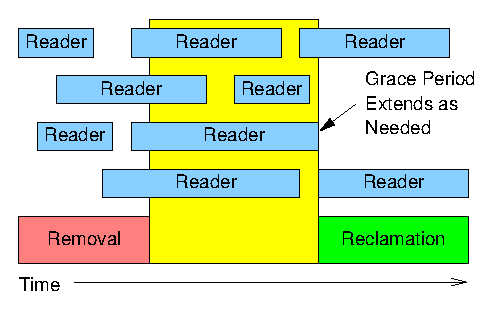
\includegraphics{appendix/rcuimpl/GracePeriodGood}}
\caption{Good Grace Period From Correct RCU}
\label{app:rcuimpl:Good Grace Period From Correct RCU}
\end{figure}

RCU 구현은 이 grace period 를 연장해야 하는데,
Figure~\ref{app:rcuimpl:Good Grace Period From Correct RCU} 에 보여진 것과 같은
형태가 될 수 있겠습니다.
짧게 말해서, 이 RCU 구현은 특정 grace period 의 시작 시점에서 진행 중이던 모든
RCU read-side 크리티컬 섹션은 해당 grace period 가 완료되기 전에 메모리
오퍼레이션들 등의 모든 것이 완전히 종료되었음을 보장해야 합니다.
이 점은 RCU 검증이 집중될 수 있게 해줍니다: 컴파일러나 CPU 가 RCU 구현이 한
일을 무효화 시키는 것을 막도록 충분히 배리어를 써서 하나의 grace period 의 시작
시점에 진행 중이던 RCU read-side 크리티컬 섹션은 모두 해당 grace period 가
종료되기 전에 끝나는 것을  보이는 겁니다.
\iffalse

It must extend the grace period, perhaps as shown in
Figure~\ref{app:rcuimpl:Good Grace Period From Correct RCU}.
In short, the RCU implementation must ensure that any
RCU read-side critical sections in progress at the start of a given grace
period have completely finished, memory operations and all, before that
grace period is permitted to complete.
This fact allows RCU validation to be extremely focused: simply demonstrate
that any RCU read-side critical section in progress at the beginning of
a grace period must terminate before that grace period ends, along with
sufficient barriers to prevent either the compiler or the CPU from undoing
the RCU implementation's work.
\fi

\subsection{Overview of Preemptible RCU Algorithm}
\label{app:rcuimpl:Overview of Preemptible RCU Algorithm}

이 섹션은 preemptible RCU 의 특정 구현에 집중합니다.
많은 다른 구현들이 있을 수 있겠지만, 그에 대해선 다른
곳~\cite{PaulEMcKenney2006b,PaulMcKenney05b} 에서 다루어졌습니다.
이 글은 이 특정 구현의 일반적인 방법들과 데이터 구조, grace-period state
machine, 그리고 read-side 기능들에 대한 파악에 집중합니다.
\iffalse

This section focuses on a specific implementation of preemptible RCU.
Many other implementations are possible, and are described
elsewhere~\cite{PaulEMcKenney2006b,PaulMcKenney05b}.
This article focuses on this specific implementation's
general approach, the data structures,
the grace-period state machine, and a walk through the read-side primitives.
\fi

\subsubsection{General Approach}
\label{app:rcuimpl:General Approach}

\begin{figure}[htb]
\centering
\resizebox{3in}{!}{\includegraphics{appendix/rcuimpl/RCUpreemptListsCompare}}
\caption{Classic vs. Preemptible RCU Callback Processing}
\label{app:rcuimpl:Classic vs. Preemptible RCU Callback Processing}
\end{figure}

이 preemptible RCU 구현은 \co{rcu_read_lock()} 과 \co{rcu_read_unlock()} 에
메모리 배리어를 필요로 하지 않기 때문에, 다단계 grace-period 탐지 알고리즘이
필요합니다.
콜백들을 위한 (기존의 RCU 구현들을 위해선 충분했던) 하나의 \co{wait} queue 를
사용하는 대신에, 이 구현은 \co{wait} 큐들의 배열을 사용해서 RCU 콜백들이 이
배열의 각 원소에 차례차례 enqueue 될 수 있게 합니다.
콜백의 흐름에 있어서의 이 차이가
Figure~\ref{app:rcuimpl:Classic vs. Preemptible RCU Callback Processing}
에 grace period 당 두개의 waitlist stage 들을 갖는 (반면, 2007년 9월 10일의 -rt
로의 패치~\cite{PaulEMcKenney2007PreemptibleRCUPatch} 는 네개의 waitlist stage
를 사용합니다) preemptible RCU 구현에 대해 그려져 있습니다.

Grace period 당 두개의 stage 를 갖기 때문에, 한쌍의 stage 들은 하나의 완전한
grace period 를 구성합니다.
비삿하게, grace period 당 네개의 stage 를 갖는 구현에서는 네개의 stage 의
연속이 하나의 완전한 grace period 를 구성합니다.
\iffalse

Because this implementation of preemptible RCU does not require memory
barriers in \co{rcu_read_lock()} and \co{rcu_read_unlock()},
a multi-stage grace-period detection algorithm is required.
Instead of using a single \co{wait} queue of callbacks
(which has sufficed for earlier RCU implementations), this implementation
uses an array of \co{wait} queues, so that RCU callbacks
are enqueued on each element of this array in turn.
This difference in callback flow is shown in
Figure~\ref{app:rcuimpl:Classic vs. Preemptible RCU Callback Processing}
for a preemptible RCU implementation with two waitlist stages per grace period
(in contrast,
the September 10 2007 patch to -rt~\cite{PaulEMcKenney2007PreemptibleRCUPatch}
uses four waitlist stages).

Given two stages per grace period, any pair of
stages forms a full grace period.
Similarly, in an implementation with four stages per grace period,
any sequence of four stages would form a full grace period.
\fi

\begin{figure}[htb]
\centering
\resizebox{3in}{!}{\includegraphics{appendix/rcuimpl/RCUpreemptCounterFlip}}
\caption{Preemptible RCU Counter Flip Operation}
\label{app:rcuimpl:Preemptible RCU Counter Flip Operation}
\end{figure}

언제 하나의 grace-period stage 가 끝날 수 있는지 판단하기 위해, preemptible RCU
는 진행중인 RCU read-side 크리티컬 섹션들을 추적하는 두개의 원소로 구성된
per-CPU \co{rcu_flipctr} 배열을 사용합니다.
특정 CPU 의 \co{rcu_flipctr} 배열의 하나의 원소는 오래된 RCU read-side 크리티컬
섹션들, 달리 말하자면 현재의 grace-period stage 보다 먼저 시작된 크리티컬
섹션들을 추적합니다.
다른 원소는 새로운 RCU read-side 크리티컬 섹션들을 추적하는데, 이것들은 현재
grace-period stage 중간에 시작된 것들입니다.
이 배열의 원소들은 새로운 grace-period stage 각각의 시작 때마다 그 역할을
바꾸는데,
Figure~\ref{app:rcuimpl:Preemptible RCU Counter Flip Operation} 에 그 모습이
그려져 있습니다.
\iffalse

To determine when a grace-period stage can end,
preemptible RCU uses a per-CPU two-element \co{rcu_flipctr} array
that tracks in-progress RCU read-side critical sections.
One element of a given CPU's \co{rcu_flipctr} array tracks
old RCU read-side critical sections, in other words, critical sections
that started before the current grace-period stage.
The other element tracks new RCU read-side critical
sections, namely those starting during the current grace-period stage.
The array elements switch roles at the beginning of each new grace-period
stage, as shown in
Figure~\ref{app:rcuimpl:Preemptible RCU Counter Flip Operation}.
\fi

앞의 그림의 왼쪽의 첫번째 stage 동안, \co{rcu_flipctr[0]} 는 새로운 RCU
read-side 크리티컬 섹션들을 추적하고, 따라서 \co{rcu_read_lock()} 에 의해 그
값이 증가하고 \co{rcu_read_unlock()} 에 의해 그 값이 감소합니다.
비슷하게, \co{rcu_flipctr[1]} 은 오래된 (앞의 stage 동안 시작된) RCU read-side
크리티컬 섹션들을 추적하고, 따라서 \co{rcu_read_unlock()} 에 의해 그 값이
감소되고 결코 그 값이 증가하지 않습니다.
\iffalse

During the first stage on the left-hand side of the above figure,
\co{rcu_flipctr[0]} tracks the new
RCU read-side critical sections, and is therefore incremented by
\co{rcu_read_lock()} and decremented by \co{rcu_read_unlock()}.
Similarly, \co{rcu_flipctr[1]} tracks the old RCU read-side
critical sections (those that started during earlier stages), and
is therefore decremented by \co{rcu_read_unlock()} and never
incremented at all.
\fi

각 CPU 의 \co{rcu_flipctr[1]} 원소는 결코 그 값이 증가되지 않기 때문에, 모든
CPU 들의 그 원소의 값의 합은 결국은 0이 됩니다, RCU read-side 크리티컬 섹션
중간의 preemption 은 개별적 카운터가 0이 아니게 놔두거나 심지어 음수를 만들
수도 있겠지만 말입니다.
예를 들어, 하나의 task 가 한 CPU 위에서 \co{rcu_read_lock()} 을 호출했고,
preemption 당한 후, 다른 CPU 에서 다시 시작되어서 \co{rcu_read_unlock()} 을
호출했다고 생각해 보세요.
첫번째 CPU 의 카운터는 +1 될것이고 두번째 CPU 의 카운터는 -1 됩니다만, 그 합은
0이 됩니다.
Preemption 의 가능성에 관계 없이, 이 카운터 원소들의 합이 0이 된다면, 앞의
그림의 오른쪽에 보여진 것처럼 다음 grace-period stage 로 넘어가도 안전합니다.
\iffalse

Because each CPU's old \co{rcu_flipctr[1]} elements are never
incremented, their sum across all CPUs must eventually go to zero,
although preemption in the midst of an RCU read-side critical section might
cause any individual counter to remain non-zero or even to go negative.
For example, suppose that a task calls \co{rcu_read_lock()} on
one CPU, is preempted, resumes on another CPU, and then calls
\co{rcu_read_unlock()}.
The first CPU's counter will then be +1 and the second CPU's counter
will be -1, however, they will still sum to zero.
Regardless of possible preemption, when the sum of the old counter
elements does go to zero, it is safe to move to the next grace-period
stage, as shown on the right-hand side of the above figure.
\fi

이 두번째 stage 에서, 각 CPU 의 \co{rcu_flipctr} 카운터 배열의 원소들은 그
역할을 서로 바꿉니다.
\co{rcu_flipctr[0]} 카운터는 이제 오래된 RCU read-side 크리티컬 섹션, 달리 말해
grace period stage 0 동안 시작된 것들을 추적합니다.
비슷하게, \co{rcu_flipctr[1]} 카운터는 이제 grace period stage 1 안에서 시작된
새로운 RCU read-side 크리티컬 섹션들을 추적합니다.
따라서, \co{rcu_read_lock()} 은 이제 \co{rcu_flipctr[1]} 의 값을 증가시키며,
\co{rcu_read_unlock()} 은 여전히 각 카운터의 값을 감소시킵니다.
특히, \co{rcu_read_lock()} 이 grace-period stage 0 (이 시점에선 과거의 stage)
동안 수행되었다면, \co{rcu_read_unlock()} 은 \co{rcu_flipctr[0]} 의 값을
감소시키지만, \co{rcu_read_lock()} 이 grace-period stage 1 (새로운 stage) 동안
수행되었다면, \co{rcu_read_unlock()} 은 \co{rcu_flipctr[1]} 의 값을 감소시켜야
합니다.
\iffalse

In this second stage, the elements of each CPU's \co{rcu_flipctr}
counter array switch roles.
The \co{rcu_flipctr[0]} counter now tracks the old RCU read-side
critical sections, in other words, the ones that started during
grace period stage 0.
Similarly, the \co{rcu_flipctr[1]} counter now tracks the new
RCU read-side critical sections that start in grace period stage 1.
Therefore, \co{rcu_read_lock()} now increments
\co{rcu_flipctr[1]}, while \co{rcu_read_unlock()} still
might decrement either counter.
Specifically, if the matching \co{rcu_read_lock()} executed
during grace-period stage 0 (the old stage at this point), then
\co{rcu_read_unlock()} must decrement \co{rcu_flipctr[0]},
but if the matching \co{rcu_read_lock()} executed during
grace-period stage 1 (the new stage), then \co{rcu_read_unlock()}
must instead decrement \co{rcu_flipctr[1]}.
\fi

여기서의 핵심은 과거의 RCU read-side 크리티컬 섹션들을 추적하는 모든
\co{rcu_flipctr} 원소들이 확실히 감소되어야 한다는 겁니다.
따라서, 일단 이 과거의 것들에 대한 카운터의 합이 0이 된다면, 이는 바뀔 수
없습니다.

\co{rcu_read_lock()} 기능은 \co{rcu_flipctr} 배열을 인덱스 하기 위해 현재
grace-period 카운터의 가장 바닥 bit (\co{rcu_ctrlblk.completed & 0x1}) 을
사용하고, 이 인덱스를 task 구조체 안에 기록해 둡니다.
여기 짝을 맞추는 \co{rcu_read_unlock()} 은 이 기록된 값을 \co{rcu_read_lock()}
이 값 증가시킨 것에 걸맞는 카운터의 값을 감소시킨다는 것을 보장하기 위해
사용합니다.
물론, 이 RCU read-side 크리팈러 섹션이 preemption 당했다면,
\co{rcu_read_unlock()} 은 짝이 맞는 \co{rcu_read_lock()} 이 값을 증가시킨
카운터가 아니라, 다른 CPU 에 속한 카운터의 값을 감소시킬 수도 있습니다.
\iffalse

The critical point is that all \co{rcu_flipctr} elements
tracking the old RCU read-side critical sections must strictly decrease.
Therefore, once the sum of these old counters reaches zero,
it cannot change.

The \co{rcu_read_lock()} primitive uses the bottom
bit of the current grace-period counter
(\co{rcu_ctrlblk.completed & 0x1}) to index the
\co{rcu_flipctr} array,
and records this index in the task structure.
The matching \co{rcu_read_unlock()} uses this recorded
value to ensure that it decrements a counter corresponding to
the one that the matching \co{rcu_read_lock()} incremented.
Of course, if the RCU read-side critical section has been preempted,
\co{rcu_read_unlock()} might be decrementing the counter
belonging to a different CPU than the one whose counter was incremented
by the matching \co{rcu_read_lock()}.
\fi

각각의 CPU 는 또한 \co{rcu_flip_flag} 와 \co{rcu_mb_flag} per-CPU 변수들을 갖고
있습니다.
\co{rcu_flip_flag} 변수는 각 grace-period stage 의 시작을 동기화 시키는 데에
사용됩니다: 일단 특정 CPU 가 \co{rcu_flip_flag} 에 응답했다면, 이제 과거의
grace-period stage 에 연관된 \co{rcu_flip} 배열의 원소의 값을 증가시키는걸
중단해야 합니다.
이 카운터의 값 (\co{rcu_ctrlblk.completed}) 을 증가시키는 CPU 는 각 CPU 의
\co{rcu_mb_flag} 의 값을 \co{rcu_flipped} 로 바꿉니다만, 특정 \co{rcu_mb_flag}
는 연관된 CPU 에 의해서만 \co{rcu_flip_seen} 으로 되바뀔 겁니다.
\iffalse

Each CPU also maintains \co{rcu_flip_flag} and
\co{rcu_mb_flag} per-CPU variables.
The \co{rcu_flip_flag} variable is used to synchronize the
start of each grace-period stage: once a given CPU has responded
to its \co{rcu_flip_flag}, it must refrain from incrementing
the \co{rcu_flip} array element that now corresponds to
the old grace-period stage.
The CPU that advances the counter (\co{rcu_ctrlblk.completed})
changes the value of each CPU's \co{rcu_mb_flag} to
\co{rcu_flipped}, but a given \co{rcu_mb_flag}
may be changed back to \co{rcu_flip_seen} only by
the corresponding CPU.
\fi

\co{rcu_mb_flag} 변수는 각 CPU 가 각 grace-period stage 의 끝에서 메몰
비래이러르 실행하도록 강제하는데에 사용됩니다.
이런 메모리 배리어들은 주어진 grace-period stage 에서 끝나는 RCU read-side
크리티컬 섹션들로부터의 메모리 접근이 이 stage 의 종료 전으로 순서잡힐 것을
보장하는데 필요합니다.
이 방법은 RCU read-side 크리티컬 섹션의 시작과 끝에 비싼 메모리 배리어를 실제로
수행하지 않고도 수행한 것과 같은 효과를 얻게 해줍니다.
\co{rcu_mb_flag} 는 과거의 것들의 카운터의 합이 0이 되는 것을 파악하는 CPU 에
의해 \co{rcu_mb_needed} 로 설정됩니다만, 해당 \co{rcu_mb_flag} 는 연관된 CPU 에
의해서만, 메모리 배리어를 수행한 후에만 \co{rcu_mb_done} 으로 되돌려집니다.
\iffalse

The \co{rcu_mb_flag} variable is used to force each CPU to
execute a memory barrier at the end of each grace-period stage.
These memory barriers are required to ensure that memory accesses from
RCU read-side critical sections ending in a given grace-period stage
are ordered before the end of that stage.
This approach gains the benefits memory barriers at the
beginning and end of each RCU read-side critical section without
having to actually execute all those costly barriers.
The \co{rcu_mb_flag} is set to \co{rcu_mb_needed} by
the CPU that detects that the sum of the old counters is zero,
but a given \co{rcu_mb_flag} is changed back to
\co{rcu_mb_done} only by the corresponding CPU, and even
then only after executing a memory barrier.
\fi

\subsubsection{Data Structures}
\label{app:rcuimpl:Data Structures}

이 섹션은 preemptible RCU 의 주요 데이터 구조인
\co{rcu_ctrlblk}, \co{rcu_data}, \co{rcu_flipctr},
\co{rcu_try_flip_state}, \co{rcu_try_flip_flag}, 그리고
\co{rcu_mb_flag} 를 설명합니다.
\iffalse

This section describes preemptible RCU's major data structures, including
\co{rcu_ctrlblk}, \co{rcu_data}, \co{rcu_flipctr},
\co{rcu_try_flip_state}, \co{rcu_try_flip_flag}, and
\co{rcu_mb_flag}.
\fi

\paragraph{{\tt rcu\_ctrlblk}}
\label{app:rcuimpl:rcu_ctrlblk}

\co{rcu_ctrlblk} 구조체는 전역적으로, grace-period 처리를 보호하는 락
(\co{filplock}) 과 global grace-period 카운터 (\co{completed}) 를 보호하는 락을
잡고 수정됩니다.
\co{completed} 의 가장 아래쪽 bit 은 \co{rcu_read_lock()} 이 어떤 카운터 집합의
값을 증가시킬지 결정하는데 사용됩니다.
\iffalse

The \co{rcu_ctrlblk} structure is global, and holds the lock
that protects grace-period processing (\co{fliplock}) as well
as holding the global grace-period counter (\co{completed}).
The least-significant bit of \co{completed} is used by
\co{rcu_read_lock()} to select which set of counters to increment.
\fi

\paragraph{{\tt rcu\_data}}
\label{app:rcuimpl:rcu_data}

\co{rcu_data} 구조체는 per-CPU 구조체로, 다음과 같은 필드들을 갖습니다:
\iffalse

The \co{rcu_data} structure is a per-CPU structure, and
contains the following fields:
\fi

\begin{itemize}
\item	\co{lock} 은 이 구조체의 나머지 필드들을 보호합니다.
\item	\co{completed} 는 CPU-local 한 활동들을 \co{rcu_ctrlblk} 의 글로벌
	카운터들과 동기화 시키는데에 사용됩니다.
\item	\co{waitlistcount} 는 비어있지 않은 wait-list 의 수를 세는데에
	사용됩니다.
	이 필드는 이 CPU 가 처리해야할 RCU 에 관련된 일을 가지고 있는지
	파악하는걸 돕는데에 \co{rcu_pending()} 에 의해 사용됩니다.
\item	\co{nextlist}, \co{nextail}, \co{waitlist},
	\co{waittail}, \co{donelist}, 그리고
	\co{donetail} 은 grace period 의 종료 시점에 호출되기를 기다리고 있는
	RCU 콜백들로 구성된 리스트들을 형성합니다.
	각각의 리스트는 tail 포인터를 가지고 있어서, $O\left(1\right)$ 삽입을
	허용합니다.
	이 RCU 콜백들은 이 리스트들을 통해 아래에 보여진 것처럼 흘러갑니다.
\item	\co{rcupreempt_trace} 는 통계를 누적합니다.
\iffalse

\item	\co{lock} guards the remaining fields in this structure.
\item	\co{completed} is used to synchronize CPU-local
	activity with the global counter in \co{rcu_ctrlblk}.
\item	\co{waitlistcount} is used to maintain a count of the
	number of non-empty wait-lists.
	This field is used by \co{rcu_pending()} to help determine
	if this CPU has any RCU-related work left to be done.
\item	\co{nextlist}, \co{nextail}, \co{waitlist},
	\co{waittail}, \co{donelist}, and
	\co{donetail} form lists containing
	RCU callbacks that are waiting for invocation at the end
	of a grace period.
	Each list has a tail pointer, allowing $O\left(1\right)$ appends.
	The RCU callbacks flow through these lists as shown below.
\item	\co{rcupreempt_trace} accumulates statistics.
\fi
\end{itemize}

\begin{figure}[htb]
\centering
\resizebox{1.5in}{!}{\includegraphics{appendix/rcuimpl/RCUpreemptLists}}
\caption{Preemptible RCU Callback Flow}
\label{app:rcuimpl:Preemptible RCU Callback Flow}
\end{figure}

Figure~\ref{app:rcuimpl:Preemptible RCU Callback Flow}
는 RCU 콜백들이 \co{rcu_data} 구조체의 리스트들을 \co{call_rcu()} 를 통한
생성부터 \co{rcu_process_callbacks()} 를 통한 호출까지 어떻게 흘러가는지
보입니다.
파란색 화살표는 각각 grace-period state machine 을 통한 이동을 나타내는데, 뒤의
섹션에서 이에 대해 설명합니다.
\iffalse

Figure~\ref{app:rcuimpl:Preemptible RCU Callback Flow}
shows how RCU callbacks flow through a given
\co{rcu_data} structure's lists, from creation by
\co{call_rcu()} through invocation by
\co{rcu_process_callbacks()}.
Each blue arrow represents one pass by the grace-period state machine,
which is described in a later section.
\fi



\paragraph{{\tt rcu\_flipctr}}
\label{app:rcuimpl:rcu_flipctr}

앞에서도 이야기했듯이, \co{rcu_flipctr} per-CPU 카운터 배열은 RCU read-side
크리티컬 섹션들을 추적하는 카운터 쌍들을 담습니다.
이 배열의 어떤 카운터든 음수가 될 수 있는데, 예를 들면 한 task 가 RCU read-side
크리티컬 센션 내에서 다른 CPU 로 옮겨가거나 하는 경우입니다.
하지만, 이 카운터들의 값의 합은 연관된 grace period 동안은 양수로 유지될
것이며, 이 grace period 의 종료 시점에서는 0이 될겁니다.
\iffalse

As noted earlier, the \co{rcu_flipctr}
per-CPU array of counters contains the
counter pairs that track outstanding RCU read-side critical sections.
Any given counter in this array can go negative, for example, when
a task is migrated to a different CPU in the middle of an RCU
read-side critical section.
However, the sum of the counters will
still remain positive throughout the corresponding grace period, and will
furthermore go to zero at the end of that grace period.
\fi

\paragraph{{\tt rcu\_try\_flip\_state}}
\label{app:rcuimpl:rcu_try_flip_state}

\co{rcu_try_flip_state} 변수는 다음 센션에서 설명하는대로 grace-period state
machine 의 현재 상태를 추적합니다.
\iffalse

The \co{rcu_try_flip_state} variable tracks the current state of
the grace-period state machine, as described in the next section.
\fi

\paragraph{{\tt rcu\_try\_flip\_flag}}
\label{app:rcuimpl:rcu_try_flip_flag}

\co{rcu_try_flip_flag} per-CPU 변수는 grace-period 캉누터가 최근에 그 값을
증가시킨데 연관된 CPU 를 알리며 해당 CPU 의 확인을 기록하기도 합니다.
일단 어떤 CPU 가 카운터 뒤집기를 확인하면, 해당 CPU 에서 \co{rcu_read_lock()}
에 의해 취해지는 후속의 동작들은 해당 grace-period 카운터의 새로운 값을 가져야
하는데, 특히 \co{rcu_read_lock()} 내에서 \co{rcu_flipctr} 의 값을 증가시킬 때가
그렇습니다.
\iffalse

The \co{rcu_try_flip_flag} per-CPU variable alerts the corresponding
CPU that the grace-period counter has recently been incremented, and
also records that CPU's acknowledgment.
Once a given CPU has acknowledged the counter flip, all subsequent actions
taken by \co{rcu_read_lock()} on that CPU must account for the
new value of the grace-period counter, in particular, when incrementing
\co{rcu_flipctr} in \co{rcu_read_lock()}.
\fi

\paragraph{{\tt rcu\_mb\_flag}}
\label{app:rcuimpl:rcu_mb_flag}

\co{rcu_mb_flag} per-CPU 변수는 grace-period state machine 이 진행될 수 있도록
하기 위해 메모리 배리어를 반드시 수행해야 하는, 연관된 CPU 를 알리며, 또한 해당
CPU 의 확인을 기록합니다.
일단 어떤 CPU 가 메모리 배리어를 수행하면, RCU read-side 크리티컬 섹션 앞의
모든 메모리 오퍼레이션들은 연관된 grace period 뒤의 코드에 보여질 겁니다.
\iffalse

The \co{rcu_mb_flag} per-CPU variable alerts the corresponding
CPU that it must execute a memory barrier in order for the grace-period
state machine to proceed, and also records that CPU's acknowledgment.
Once a given CPU has executed its memory barrier, the memory operations
of all prior RCU read-side critical will be visible to any code sequenced
after the corresponding grace period.
\fi


\subsubsection{Grace-Period State Machine}
\label{app:rcuimpl:Grace-Period State Machine}

이 섹션은 grace-period state machine 에 의해 수행되는 state 들에 대한 개괄을
제공하고 관련된 코드들을 살펴봅니다.
\iffalse

This section gives an overview of the states executed by the grace-period
state machine, and then walks through the relevant code.
\fi

\paragraph{Grace-Period State Machine Overview}
\label{app:rcuimpl:Grace-Period State Machine Overview}

이 상태 (\co{rcu_try_flip_state} 에 기록되어짐) 는 다음과 같은 값들을 가질 수
있습니다:
\iffalse

The state (recorded in \co{rcu_try_flip_state})
can take on the following values:
\fi

\begin{itemize}
\item	\co{rcu_try_flip_idle_state}:  어떤 RCU grace-period 활동도 없기에
	Grace-period state machine 이 idle 상태에 있음.
	\co{rcu_ctrlblk.completed} grace-period 카운터는 이 상태로부터 빠져나갈
	때마다 값이 증가되고, 모든 per-CPU \co{rcu_flip_flag} 변수들은
	\co{rcu_flipped} 로 설정됩니다.
\item	\co{rcu_try_flip_waitack_state}:
	모든 CPU 들이 각자의 \co{rcu_flip_fflag} 변수를 \co{rcu_flip_seen} 으로
	설정함으로써 기존 state 의 증가를 보았음을 보고하기를 기다리는 상태.
	일단 모든 CPU 들이 이렇게 보고를 하게 되면, 우린 과거의 카운터 집합은
	더이상 값 증가할 수 없음을 알게 됩니다.
\item	\co{rcu_try_flip_waitack_state}:
	기존 카운터들의 값의 합이 0이 되길 기다리는 상태.
	일단 카운터들의 값의 합이 0이 되면, 모든 per-CPU \co{rcu_mb_flag}
	변수들은 \co{rcu_mb_needed} 로 설정됩니다.
\item	\co{rcu_try_flip_waitmb_state}:
	모든 CPU 들이 각자의 \co{rcu_mb_flag} 변수의 값을 \co{rcu_mb_done} 으로
	설정함으로써 메모리 배리어 인스트럭션을 수행했음을 알리기를 기다리는
	상태.
	일단 모든 CPU 들이 메모리 배리어 인스트럭션을 수행하면, 연관된 grace
	period 의 시작 전에 시작된 read-side 크리티컬 섹션에 의해 만들어진
	변경사항은 모든 CPU 들이 볼 수 있을 것임이 완화된 순서규칙의 기계에서도
	보장됩니다.
\iffalse

\item	\co{rcu_try_flip_idle_state}:  the grace-period state
	machine is idle due to there being no RCU grace-period activity.
	The \co{rcu_ctrlblk.completed} grace-period counter
	is incremented upon exit from this state, and all of the
	per-CPU \co{rcu_flip_flag} variables are set
	to \co{rcu_flipped}.
\item	\co{rcu_try_flip_waitack_state}:
	waiting for all CPUs to acknowledge that they have seen the
	previous state's increment, which they do by setting their
	\co{rcu_flip_flag} variables to \co{rcu_flip_seen}.
	Once all CPUs have so acknowledged, we know that the old
	set of counters can no longer be incremented.
\item	\co{rcu_try_flip_waitzero_state}:
	waiting for the old counters to sum to zero.
	Once the counters sum to zero, all of the per-CPU
	\co{rcu_mb_flag} variables are set to
	\co{rcu_mb_needed}.
\item	\co{rcu_try_flip_waitmb_state}:
	waiting for all CPUs to execute a memory-barrier instruction,
	which they signify by setting their \co{rcu_mb_flag}
	variables to \co{rcu_mb_done}.
	Once all CPUs have done so, all CPUs are guaranteed to see
	the changes made by any RCU read-side critical section that
	started before the beginning of the corresponding grace period,
	even on weakly ordered machines.
\fi
\end{itemize}

\begin{figure}[htb]
\centering
\resizebox{3in}{!}{\includegraphics{appendix/rcuimpl/RCUpreemptStates}}
\caption{Preemptible RCU State Machine}
\label{app:rcuimpl:Preemptible RCU State Machine}
\end{figure}

Grace period state machine 은
Figure~\ref{app:rcuimpl:Preemptible RCU State Machine}
에 보여진 것처럼 이 상태들을 순차적으로 돌아갑니다.
\iffalse

The grace period state machine cycles through these states sequentially,
as shown in
Figure~\ref{app:rcuimpl:Preemptible RCU State Machine}.
\fi

\begin{figure}[htb]
\centering
\resizebox{3in}{!}{\includegraphics{appendix/rcuimpl/RCUpreemptTimeline}}
\caption{Preemptible RCU State Machine Timeline}
\label{app:rcuimpl:Preemptible RCU State Machine Timeline}
\end{figure}

Figure~\ref{app:rcuimpl:Preemptible RCU State Machine Timeline}
는 이 state machine 이 어떻게 시간의 흐름에 따라 동작하는지 보입니다.
상태들은 이 그림의 왼쪽에 보여져 있고 연관된 이벤트들이 시간의 흐름에 따라
보여져 있는데, 시간은 아래쪽으로 흐르고 있습니다.
우리는 뒤의 섹션에서 이 알고리즘을 검증할 때에 이 그림을 상세히 설명할 겁니다.

그 전까지는, 여기에 알아둘 중요한 사항들이 있으니 알아두시기 바랍니다:
\iffalse

Figure~\ref{app:rcuimpl:Preemptible RCU State Machine Timeline}
shows how the state machine operates over time.
The states are shown along the figure's left-hand side and the relevant events
are shown along the timeline, with time proceeding in the downward direction.
We will elaborate on this figure when we validate the algorithm in
a later section.

In the meantime, here are some important things to note:
\fi

\begin{enumerate}
\item	\co{rcu_ctrlblk.completed} 카운터의 값 증가는 파란 타원으로 표시된
	것처럼 다른 시간에 다른 CPU 들에 의해 관측되어질 수 있습니다.  하지만,
	해당 CPU 가 이 값 증가를 알아챈 다음에는, 새로운 카운터를 사용해야
	합니다.
	따라서, 일단 모든 CPU 들이 알아챘음을 알린다면, 과거의 카운터의 값은
	감소만 될 수 있습니다.
\item	특정 CPU 는 이 카운터의 값 증가를 알기 전까지만 콜백 리스트들을
	진행시킬 수 있습니다.
\item	파란 타원은 메모리 오퍼레이션 재배치가 다른 CPU 들이 값 증가를 다른
	시간에 볼 수 있음을 알립니다.
	이는 특정 CPU 는 어떤 다른 CPU 가 이 카운터의 새로운 값을 해당 카운터가
	진짜로 증가하기 전에 사용해서 이 구간을 건너뛰었다고 믿을 수도 있음을
	의미합니다.
	실제로, 이론상으로는, 특정 CPU 는 \co{rcu_ctrlblk.completed} 카운터의
	다음의 값 증가를 기존의 메모리 배리어가 쳐진 시점만큼 빠른 시간에
	볼수도 있습니다.
	(이 문장은 매우 부정확함을 알아두시기 바랍니다.
	메모리 배리어에 대한 올바름의 증명을 하고자 한다면,
	Appendix~\ref{app:rcuimpl:Formal Validation} 를 보기 바랍니다.
\iffalse

\item	The increment of the \co{rcu_ctrlblk.completed} counter
	might be observed at different times by different CPUs, as
	indicated by the blue oval.  However, after a given
	CPU has acknowledged the increment, it is required to
	use the new counter.
	Therefore, once all CPUs have acknowledged, the old counter
	can only be decremented.
\item	A given CPU advances its callback lists just before
	acknowledging the counter increment.
\item	The blue oval represents the fact that memory reordering
	might cause different CPUs to see the increment at
	different times.
	This means that a given CPU might believe that some
	other CPU has jumped the gun, using the new value of the counter
	before the counter was actually incremented.
	In fact, in theory, a given CPU might see the next increment of the
	\co{rcu_ctrlblk.completed} counter as early as
	the last preceding memory barrier.
	(Note well that this sentence is very imprecise.
	If you intend to do correctness proofs involving memory barriers,
	please see Appendix~\ref{app:rcuimpl:Formal Validation}.
\fi
\item	\co{rcu_read_lock()} 은 어떤 메모리 배리어도 포함하고 있지 않기 때문에,
	연관된 RCU read-side 크리티컬 섹션들은 해당 CPU 에 의해
	\co{rcu_read_unlock()} 을 뒤따르도록 재배치 될수도 있습니다.
	따라서, 이 RCU read-side 크리티컬 섹션들의 행동들이 실제로 완료되었음을
	보장하기 위해 메모리 배리어가 필요합니다.
\item	이어서 보게 되겠지만, 서로 다른 CPU 들이 카운터의 flip 을 서로 다른
	시간에 볼 수 있다는 사실은 state machine 을 통한 한번의 횡단은 grace
	period 에 충분치 않음을 의미합니다: 여러번의 횡단이 필요합니다.
\iffalse

\item	Because \co{rcu_read_lock()} does not contain any
	memory barriers, the corresponding RCU read-side critical
	sections might be reordered by the CPU to follow the
	\co{rcu_read_unlock()}.
	Therefore, the memory barriers are required to ensure
	that the actions of the RCU read-side critical sections
	have in fact completed.
\item	As we will see, the fact that different CPUs can see the
	counter flip happening at different times means that a
	single trip through the state machine is not sufficient
	for a grace period: multiple trips are required.
\fi
\end{enumerate}

\paragraph{Grace-Period State Machine Walkthrough}
\label{app:rcuimpl:Grace-Period State Machine Walkthrough}

\begin{figure}[tbp]
{ \scriptsize
\begin{verbatim}
  1 void rcu_check_callbacks(int cpu, int user)
  2 {
  3   unsigned long flags;
  4   struct rcu_data *rdp = RCU_DATA_CPU(cpu);
  5
  6   rcu_check_mb(cpu);
  7   if (rcu_ctrlblk.completed == rdp->completed)
  8     rcu_try_flip();
  9   spin_lock_irqsave(&rdp->lock, flags);
 10   RCU_TRACE_RDP(rcupreempt_trace_check_callbacks, rdp);
 11   __rcu_advance_callbacks(rdp);
 12   spin_unlock_irqrestore(&rdp->lock, flags);
 13 }
\end{verbatim}
}
\caption{{\tt rcu\_check\_callbacks()} Implementation}
\label{fig:app:rcuimpl:rcu_check_callbacks() Implementation}
\end{figure}

이 섹션은 scheduling-clock 인터럽트에서 irq (그리고 preemption) 가 비활성화된
채로 \co{rcu_check_callbacks()} 를 호출하는, RCU grace-period state machine 을
구현하는 C 코드를 살펴봅니다.
이 함수는
Figure~\ref{fig:app:rcuimpl:rcu_check_callbacks() Implementation}
에 보여지는 것처럼 구현되어 있습니다.
Line~4 는 현재의 CPU 에 연관된 \co{rcu_data} 구조체를 골라내고 line~6 는 이 CPU
가 state machine 을 \co{rcu_try_flip_waitmb_state} 상태에서 진행시키기 위해
메모리 배리어를 실행해야 하는지를 체크합니다.
Line~7 은 이 CPU 가 이미 현재 grace-period stage number 를 알고 있는지 보고,
그렇다면 line~8 에서 이 state machine 을 진행시킵니다.
Line~9 와 12 는 \co{rcu_data} 의 락을 잡고, line~11 에서는 적절하다면 콜백들을
수행시킵니다.
Line~10 에서는 \co{CONFIG_RCU_TRACE} 가 활성화 되어 있다면 RCU tracing 을 위한
통계들을 업데이트합니다.
\iffalse

This section walks through the C code that implements the RCU
grace-period state machine, which is invoked from the scheduling-clock
interrupt, which invokes \co{rcu_check_callbacks()} with
irqs (and thus also preemption) disabled.
This function is implemented as shown in
Figure~\ref{fig:app:rcuimpl:rcu_check_callbacks() Implementation}.
Line~4 selects the \co{rcu_data} structure corresponding
to the current CPU, and line~6 checks to see if this CPU needs
to execute a memory barrier to advance the state machine out of the
\co{rcu_try_flip_waitmb_state} state.
Line~7 checks to see if this CPU is already aware of the
current grace-period stage number, and line~8 attempts to advance the
state machine if so.
Lines~9 and 12 hold the \co{rcu_data}'s lock, and
line~11 advances callbacks if appropriate.
Line~10 updates RCU tracing statistics, if enabled via
\co{CONFIG_RCU_TRACE}.
\fi

\begin{figure}[tbp]
{ \scriptsize
\begin{verbatim}
  1 static void rcu_check_mb(int cpu)
  2 {
  3   if (per_cpu(rcu_mb_flag, cpu) == rcu_mb_needed) {
  4     smp_mb();
  5     per_cpu(rcu_mb_flag, cpu) = rcu_mb_done;
  6   }
  7 }
\end{verbatim}
}
\caption{{\tt rcu\_check\_mb()} Implementation}
\label{fig:app:rcuimpl:rcu_check_mb() Implementation}
\end{figure}

\co{rcu_check_mb()} 함수는
Figure~\ref{fig:app:rcuimpl:rcu_check_mb() Implementation}
에 보여진 것처럼 필요하면 메모리 배리어를 수행합니다.
Line~3 는 이 CPU 가 메모리 배리어를 수행해야 하는지 체크하고, 만약 그렇다면
line~4 에서 메모리 배리어를 실행하고 line~5 에서 state machine 을 알립니다.
이 메모리 배리어는 \co{rcu_mb_flag} 의 새로운 값을 보는 모든 CPU 는 이 CPU 에
의해 앞의 RCU read-side 크리티컬 섹션 안에서 수행된 메모리 오퍼레이션들을 보게
될 것을 보장함을 알아두시기 바랍니다.
\iffalse

The \co{rcu_check_mb()} function executes a memory barrier
as needed as shown in
Figure~\ref{fig:app:rcuimpl:rcu_check_mb() Implementation}.
Line~3 checks to see if this CPU needs to execute a memory barrier,
and, if so, line~4 executes one and line~5 informs the state
machine.
Note that this memory barrier ensures that any CPU that sees the new
value of \co{rcu_mb_flag} will also see the memory operations
executed by this CPU in any prior RCU read-side critical section.
\fi

\begin{figure}[tbp]
{ \scriptsize
\begin{verbatim}
  1 static void rcu_try_flip(void)
  2 {
  3   unsigned long flags;
  4
  5   RCU_TRACE_ME(rcupreempt_trace_try_flip_1);
  6   if (!spin_trylock_irqsave(&rcu_ctrlblk.fliplock, flags)) {
  7     RCU_TRACE_ME(rcupreempt_trace_try_flip_e1);
  8     return;
  9   }
 10   switch (rcu_try_flip_state) {
 11   case rcu_try_flip_idle_state:
 12     if (rcu_try_flip_idle())
 13       rcu_try_flip_state = rcu_try_flip_waitack_state;
 14     break;
 15   case rcu_try_flip_waitack_state:
 16     if (rcu_try_flip_waitack())
 17       rcu_try_flip_state = rcu_try_flip_waitzero_state;
 18     break;
 19   case rcu_try_flip_waitzero_state:
 20     if (rcu_try_flip_waitzero())
 21       rcu_try_flip_state = rcu_try_flip_waitmb_state;
 22     break;
 23   case rcu_try_flip_waitmb_state:
 24     if (rcu_try_flip_waitmb())
 25       rcu_try_flip_state = rcu_try_flip_idle_state;
 26   }
 27   spin_unlock_irqrestore(&rcu_ctrlblk.fliplock, flags);
 28 }
\end{verbatim}
}
\caption{{\tt rcu\_try\_flip()} Implementation}
\label{fig:app:rcuimpl:rcu_try_flip() Implementation}
\end{figure}

\co{rcu_try_flip()} 함수는
Figure~\ref{fig:app:rcuimpl:rcu_try_flip() Implementation}
에 보인 것처럼 RCU grace-period state machine 의 최고단계 구현을 합니다.
Line~6 는 global RCU state-machine lock 을 획득하려 시도하고, 실패하면
리턴합니다.
Line~5 와 7 은 (\co{CONFIG_RCU_TRACE} 가 활성화 되어 있다면) RCU-tracing 통계를
조작합니다.
Line~10 부터 26 은 state machine 을 수행하는데, 각각 해당 state 에 맞는 함수를
수행시킵니다.
그런 함수 각각은 해당 state 가 진행되야 한다면 1을, 그렇지 않다면 0을
리턴합니다.
원칙적으로, 다음 state 를 곧바로 수행될 수 있지만, 실제로는 응답시간을 줄이기
위해 그렇게 하지 않습니다.
마지막으로, line~27 에서는 line~6 에서 획득했던 global RCU state-machine lock
을 해제합니다.
\iffalse

The \co{rcu_try_flip()} function implements the top level of
the RCU grace-period state machine, as shown in
Figure~\ref{fig:app:rcuimpl:rcu_try_flip() Implementation}.
Line~6 attempts to acquire the global RCU state-machine lock,
and returns if unsuccessful.
Lines;~5 and 7 accumulate RCU-tracing statistics (again, if
\co{CONFIG_RCU_TRACE} is enabled).
Lines~10 through 26 execute the state machine,
each invoking a function specific to that state.
Each such function returns 1 if the state needs to be advanced and
0 otherwise.
In principle, the next state could be executed immediately,
but in practice we choose not to do so in order to reduce latency.
Finally, line~27 releases the global RCU state-machine lock
that was acquired by line~6.
\fi

\begin{figure}[tbp]
{ \scriptsize
\begin{verbatim}
  1 static int rcu_try_flip_idle(void)
  2 {
  3   int cpu;
  4
  5   RCU_TRACE_ME(rcupreempt_trace_try_flip_i1);
  6   if (!rcu_pending(smp_processor_id())) {
  7     RCU_TRACE_ME(rcupreempt_trace_try_flip_ie1);
  8     return 0;
  9   }
 10   RCU_TRACE_ME(rcupreempt_trace_try_flip_g1);
 11   rcu_ctrlblk.completed++;
 12   smp_mb();
 13   for_each_cpu_mask(cpu, rcu_cpu_online_map)
 14     per_cpu(rcu_flip_flag, cpu) = rcu_flipped;
 15   return 1;
 16 }
\end{verbatim}
}
\caption{{\tt rcu\_try\_flip\_idle()} Implementation}
\label{fig:app:rcuimpl:rcu_try_flip_idle() Implementation}
\end{figure}

The \co{rcu_try_flip_idle()} function is called when the
RCU grace-period state machine is idle, and is thus responsible for
getting it started when needed.
Its code is shown in
Figure~\ref{fig:app:rcuimpl:rcu_try_flip_idle() Implementation}.
Line~6 checks to see if there is any RCU grace-period work
pending for this CPU, and if not, line~8 leaves, telling
the top-level state machine to remain in the idle state.
If instead there is work to do, line~11 increments the
grace-period stage counter, line~12 does a memory barrier
to ensure that CPUs see the new counter before they see the
request to acknowledge it, and lines~13 and 14 set all of
the online CPUs' \co{rcu_flip_flag}.
Finally, line~15 tells the top-level state machine to
advance to the next state.

\begin{figure}[tbp]
{ \scriptsize
\begin{verbatim}
  1 static int rcu_try_flip_waitack(void)
  2 {
  3   int cpu;
  4
  5   RCU_TRACE_ME(rcupreempt_trace_try_flip_a1);
  6   for_each_cpu_mask(cpu, rcu_cpu_online_map)
  7     if (per_cpu(rcu_flip_flag, cpu) != rcu_flip_seen) {
  8       RCU_TRACE_ME(rcupreempt_trace_try_flip_ae1);
  9       return 0;
 10     }
 11   smp_mb();
 12   RCU_TRACE_ME(rcupreempt_trace_try_flip_a2);
 13   return 1;
 14 }
\end{verbatim}
}
\caption{{\tt rcu\_try\_flip\_waitack()} Implementation}
\label{fig:app:rcuimpl:rcu_try_flip_waitack() Implementation}
\end{figure}

The \co{rcu_try_flip_waitack()} function, shown in
Figure~\ref{fig:app:rcuimpl:rcu_try_flip_waitack() Implementation},
checks to see
if all online CPUs have acknowledged the counter flip (AKA ``increment'',
but called ``flip'' because the bottom bit, which \co{rcu_read_lock()}
uses to index the \co{rcu_flipctr} array, \emph{does} flip).
If they have, it tells the top-level grace-period state machine to
move to the next state.

Line~6 cycles through all of the online CPUs, and line~7
checks to see if the current such CPU has acknowledged the last counter
flip.
If not, line~9 tells the top-level grace-period state machine to
remain in this state.
Otherwise, if all online CPUs have acknowledged, then line~11
does a memory barrier to ensure that we don't check for zeroes before
the last CPU acknowledges.
This may seem dubious, but CPU designers have sometimes done strange
things.
Finally, line~13 tells the top-level grace-period state machine
to advance to the next state.

\begin{figure}[tbp]
{ \scriptsize
\begin{verbatim}
  1 static int rcu_try_flip_waitzero(void)
  2 {
  3   int cpu;
  4   int lastidx = !(rcu_ctrlblk.completed & 0x1);
  5   int sum = 0;
  6
  7   RCU_TRACE_ME(rcupreempt_trace_try_flip_z1);
  8   for_each_possible_cpu(cpu)
  9     sum += per_cpu(rcu_flipctr, cpu)[lastidx];
 10   if (sum != 0) {
 11     RCU_TRACE_ME(rcupreempt_trace_try_flip_ze1);
 12     return 0;
 13   }
 14   smp_mb();
 15   for_each_cpu_mask(cpu, rcu_cpu_online_map)
 16     per_cpu(rcu_mb_flag, cpu) = rcu_mb_needed;
 17   RCU_TRACE_ME(rcupreempt_trace_try_flip_z2);
 18   return 1;
 19 }
\end{verbatim}
}
\caption{{\tt rcu\_try\_flip\_waitzero()} Implementation}
\label{fig:app:rcuimpl:rcu_try_flip_waitzero() Implementation}
\end{figure}

The \co{rcu_try_flip_waitzero()} function, shown in
Figure~\ref{fig:app:rcuimpl:rcu_try_flip_waitzero() Implementation},
checks to see if
all pre-existing RCU read-side critical sections have completed,
telling the state machine to advance if so.
Lines~8 and 9 sum the counters, and line~10 checks
to see if the result is zero, and, if not, line~12 tells
the state machine to stay right where it is.
Otherwise, line~14 executes a memory barrier to ensure that
no CPU sees the subsequent call for a memory barrier before it
has exited its last RCU read-side critical section.
This possibility might seem remote, but again, CPU designers have
done stranger things, and besides, this is anything but a fastpath.
Lines~15 and 16 set all online CPUs' \co{rcu_mb_flag}
variables, and line~18 tells the state machine to advance to
the next state.

\begin{figure}[tbp]
{ \scriptsize
\begin{verbatim}
  1 static int rcu_try_flip_waitmb(void)
  2 {
  3   int cpu;
  4
  5   RCU_TRACE_ME(rcupreempt_trace_try_flip_m1);
  6   for_each_cpu_mask(cpu, rcu_cpu_online_map)
  7     if (per_cpu(rcu_mb_flag, cpu) != rcu_mb_done) {
  8       RCU_TRACE_ME(rcupreempt_trace_try_flip_me1);
  9       return 0;
 10     }
 11   smp_mb();
 12   RCU_TRACE_ME(rcupreempt_trace_try_flip_m2);
 13   return 1;
 14 }
\end{verbatim}
}
\caption{{\tt rcu\_try\_flip\_waitmb()} Implementation}
\label{fig:app:rcuimpl:rcu_try_flip_waitmb() Implementation}
\end{figure}

The \co{rcu_try_flip_waitmb()} function, shown in
Figure~\ref{fig:app:rcuimpl:rcu_try_flip_waitmb() Implementation},
checks to see
if all online CPUs have executed the requested memory barrier,
telling the state machine to advance if so.
Lines~6 and 7 check each online CPU to see if it has
done the needed memory barrier, and if not, line~9 tells
the state machine not to advance.
Otherwise, if all CPUs have executed a memory barrier, line~11
executes a memory barrier to ensure that any RCU callback invocation
follows all of the memory barriers, and line~13 tells the
state machine to advance.

\begin{figure}[tbp]
{ \scriptsize
\begin{verbatim}
  1 static void __rcu_advance_callbacks(struct rcu_data *rdp)
  2 {
  3   int cpu;
  4   int i;
  5   int wlc = 0;
  6
  7   if (rdp->completed != rcu_ctrlblk.completed) {
  8     if (rdp->waitlist[GP_STAGES - 1] != NULL) {
  9       *rdp->donetail = rdp->waitlist[GP_STAGES - 1];
 10       rdp->donetail = rdp->waittail[GP_STAGES - 1];
 11       RCU_TRACE_RDP(rcupreempt_trace_move2done, rdp);
 12     }
 13     for (i = GP_STAGES - 2; i >= 0; i--) {
 14       if (rdp->waitlist[i] != NULL) {
 15         rdp->waitlist[i + 1] = rdp->waitlist[i];
 16         rdp->waittail[i + 1] = rdp->waittail[i];
 17         wlc++;
 18       } else {
 19         rdp->waitlist[i + 1] = NULL;
 20         rdp->waittail[i + 1] =
 21           &rdp->waitlist[i + 1];
 22       }
 23     }
 24     if (rdp->nextlist != NULL) {
 25       rdp->waitlist[0] = rdp->nextlist;
 26       rdp->waittail[0] = rdp->nexttail;
 27       wlc++;
 28       rdp->nextlist = NULL;
 29       rdp->nexttail = &rdp->nextlist;
 30       RCU_TRACE_RDP(rcupreempt_trace_move2wait, rdp);
 31     } else {
 32       rdp->waitlist[0] = NULL;
 33       rdp->waittail[0] = &rdp->waitlist[0];
 34     }
 35     rdp->waitlistcount = wlc;
 36     rdp->completed = rcu_ctrlblk.completed;
 37   }
 38   cpu = raw_smp_processor_id();
 39   if (per_cpu(rcu_flip_flag, cpu) == rcu_flipped) {
 40     smp_mb();
 41     per_cpu(rcu_flip_flag, cpu) = rcu_flip_seen;
 42     smp_mb();
 43   }
 44 }
\end{verbatim}
}
\caption{{\tt \_\_rcu\_advance\_callbacks()} Implementation}
\label{fig:app:rcuimpl:__rcu_advance_callbacks() Implementation}
\end{figure}

The \co{__rcu_advance_callbacks()} function, shown in
Figure~\ref{fig:app:rcuimpl:__rcu_advance_callbacks() Implementation},
advances callbacks and acknowledges the counter flip.
Line~7 checks to see if the global \co{rcu_ctrlblk.completed}
counter has advanced since the last call by the current CPU to this
function.
If not, callbacks need not be advanced (lines~8-37).
Otherwise, lines~8 through 37 advance callbacks through the lists
(while maintaining a count of the number of non-empty lists in the
\co{wlc} variable).
In either case, lines~38 through 43 acknowledge the counter flip
if needed.

\QuickQuiz{}
	How is it possible for lines~38-43 of
	\co{__rcu_advance_callbacks()} to be executed when
	lines~7-37 have not?
	Won't they both be executed just after a counter flip, and
	never at any other time?
\QuickQuizAnswer{
	Consider the following sequence of events:
	\begin{enumerate}
	\item	CPU 0 executes lines~5-12 of
		\co{rcu_try_flip_idle()}.
	\item	CPU 1 executes \co{__rcu_advance_callbacks()}.
		Because \co{rcu_ctrlblk.completed} has been
		incremented, lines~7-37 execute.
		However, none of the \co{rcu_flip_flag} variables
		have been set, so lines~38-43 do \emph{not} execute.
	\item	CPU 0 executes lines~13-15 of
		\co{rcu_try_flip_idle()}.
	\item	Later, CPU 1 again executes \co{__rcu_advance_callbacks()}.
		The counter has not been incremented since the earlier
		execution, but the \co{rcu_flip_flag} variables have
		all been set, so only lines~38-43 are executed.
	\end{enumerate}
} \QuickQuizEnd


\subsubsection{Read-Side Primitives}
\label{app:rcuimpl:Read-Side Primitives}

This section examines the \co{rcu_read_lock()} and
\co{rcu_read_unlock()} primitives, followed by a
discussion of how this implementation deals with the fact
that these two primitives do not contain memory barriers.

\paragraph{{\tt rcu\_read\_lock()}}
\label{app:rcuimpl:rcu_read_lock()}

\begin{figure}[tbp]
{ \scriptsize
\begin{verbatim}
  1 void __rcu_read_lock(void)
  2 {
  3   int idx;
  4   struct task_struct *t = current;
  5   int nesting;
  6
  7   nesting = ACCESS_ONCE(t->rcu_read_lock_nesting);
  8   if (nesting != 0) {
  9     t->rcu_read_lock_nesting = nesting + 1;
 10   } else {
 11     unsigned long flags;
 12
 13     local_irq_save(flags);
 14     idx = ACCESS_ONCE(rcu_ctrlblk.completed) & 0x1;
 15     ACCESS_ONCE(__get_cpu_var(rcu_flipctr)[idx])++;
 16     ACCESS_ONCE(t->rcu_read_lock_nesting) = nesting + 1;
 17     ACCESS_ONCE(t->rcu_flipctr_idx) = idx;
 18     local_irq_restore(flags);
 19   }
 20 }
\end{verbatim}
}
\caption{{\tt \_\_rcu\_read\_lock()} Implementation}
\label{fig:app:rcuimpl:__rcu_read_lock() Implementation}
\end{figure}

The implementation of \co{rcu_read_lock()} is as shown in
Figure~\ref{fig:app:rcuimpl:__rcu_read_lock() Implementation}.
Line~7 fetches this task's RCU read-side critical-section nesting
counter.
If line~8 finds that this counter is non-zero,
then we are already protected by an outer
\co{rcu_read_lock()}, in which case line~9 simply increments
this counter.

However, if this is the outermost \co{rcu_read_lock()},
then more work is required.
Lines~13 and 18 suppress and restore irqs to ensure that the
intervening code is neither preempted nor interrupted by a
scheduling-clock interrupt (which runs the grace period state machine).
Line~14 fetches the grace-period counter,
line~15 increments the current counter for
this CPU, line~16 increments the nesting counter,
and line~17 records the old/new counter index so that
\co{rcu_read_unlock()} can decrement the corresponding
counter (but on whatever CPU it ends up running on).

The \co{ACCESS_ONCE()} macros force the compiler to
emit the accesses in order.
Although this does not prevent the CPU from reordering the accesses
from the viewpoint of other CPUs, it does ensure that NMI and
SMI handlers running on this CPU will see these accesses in order.
This is critically important:

\begin{enumerate}
\item	In absence of the \co{ACCESS_ONCE()} in the assignment
	to \co{idx}, the compiler would be within its rights
	to: (a) eliminate the local variable \co{idx} and
	(b) compile the increment on line~16 as a
	fetch-increment-store sequence, doing separate accesses to
	\co{rcu_ctrlblk.completed} for the fetch and the
	store.
	If the value of \co{rcu_ctrlblk.completed} had
	changed in the meantime, this would corrupt the
	\co{rcu_flipctr} values.
\item	If the assignment to \co{rcu_read_lock_nesting}
	(line~17) were to be reordered to precede the increment
	of \co{rcu_flipctr} (line~16), and if an
	NMI occurred between these two events, then an
	\co{rcu_read_lock()} in that NMI's handler
	would incorrectly conclude that it was already under the
	protection of \co{rcu_read_lock()}.
\item	If the assignment to \co{rcu_read_lock_nesting}
        (line~17) were to be reordered to follow the assignment
	to \co{rcu_flipctr_idx} (line~18), and if an
	NMI occurred between these two events, then an
	\co{rcu_read_lock()} in that NMI's handler
	would clobber \co{rcu_flipctr_idx}, possibly
	causing the matching \co{rcu_read_unlock()} to
	decrement the wrong counter.
	This in turn could result in premature ending of a
	grace period, indefinite extension of a grace period,
	or even both.
\end{enumerate}

It is not clear that the \co{ACCESS_ONCE} on the assignment to
\co{nesting} (line~7) is required.
It is also unclear whether the \co{smp_read_barrier_depends()}
(line~15) is needed: it was added to ensure that changes to index
and value remain ordered.

The reasons that irqs must be disabled from line~13 through
line~19 are as follows:

\begin{enumerate}
\item	Suppose one CPU loaded \co{rcu_ctrlblk.completed}
	(line~14), then a second CPU incremented this counter,
	and then the first CPU took a scheduling-clock interrupt.
	The first CPU would then see that it needed to acknowledge
	the counter flip, which it would do.
	This acknowledgment is a promise to avoid incrementing
	the newly old counter, and this CPU would break this
	promise.
	Worse yet, this CPU might be preempted immediately upon
	return from the scheduling-clock interrupt, and thus
	end up incrementing the counter at some random point
	in the future.
	Either situation could disrupt grace-period detection.
\item	Disabling irqs has the side effect of disabling preemption.
	If this code were to be preempted between fetching
	\co{rcu_ctrlblk.completed} (line~14) and
	incrementing \co{rcu_flipctr} (line~16),
	it might well be migrated to some other CPU.
	This would result in it non-atomically incrementing
	the counter from that other CPU.
	If this CPU happened to be executing in \co{rcu_read_lock()}
	or \co{rcu_read_unlock()} just at that time, one
	of the increments or decrements might be lost, again
	disrupting grace-period detection.
	The same result could happen on RISC machines if the preemption
	occurred in the middle of the increment (after the fetch of
	the old counter but before the store of the newly incremented
	counter).
\item	Permitting preemption in the midst
	of line~16, between selecting the current CPU's copy
	of the \co{rcu_flipctr} array and the increment of
	the element indicated by \co{rcu_flipctr_idx}, can
	result in a similar failure.
	Execution might well resume on some other CPU.
	If this resumption happened concurrently with an
	\co{rcu_read_lock()} or \co{rcu_read_unlock()}
	running on the original CPU,
	an increment or decrement might be lost, resulting in either
	premature termination of a grace period, indefinite extension
	of a grace period, or even both.
\item	Failing to disable preemption can also defeat RCU priority
	boosting, which relies on \co{rcu_read_lock_nesting}
	to determine when a given task is in an RCU read-side
	critical section.
	So, for example, if a given task is indefinitely
	preempted just after incrementing \co{rcu_flipctr},
	but before updating \co{rcu_read_lock_nesting},
	then it will stall RCU grace periods for as long as it
	is preempted.
	However, because \co{rcu_read_lock_nesting} has not
	yet been incremented, the RCU priority booster has no way
	to tell that boosting is needed.
	Therefore, in the presence of CPU-bound realtime threads,
	the preempted task might stall grace periods indefinitely,
	eventually causing an OOM event.
\end{enumerate}

The last three reasons could of course be addressed by disabling
preemption rather than disabling of irqs, but given that the first
reason requires disabling irqs in any case, there is little reason
to separately disable preemption.
It is entirely possible that the first reason might be tolerated
by requiring an additional grace-period stage, however, it is not
clear that disabling preemption is much faster than disabling
interrupts on modern CPUs.

\paragraph{{\tt rcu\_read\_unlock()}}
\label{app:rcuimpl:rcu_read_unlock()}

\begin{figure}[tbp]
{ \scriptsize
\begin{verbatim}
  1 void __rcu_read_unlock(void)
  2 {
  3   int idx;
  4   struct task_struct *t = current;
  5   int nesting;
  6
  7   nesting = ACCESS_ONCE(t->rcu_read_lock_nesting);
  8   if (nesting > 1) {
  9     t->rcu_read_lock_nesting = nesting - 1;
 10   } else {
 11     unsigned long flags;
 12
 13     local_irq_save(flags);
 14     idx = ACCESS_ONCE(t->rcu_flipctr_idx);
 15     ACCESS_ONCE(t->rcu_read_lock_nesting) = nesting - 1;
 16     ACCESS_ONCE(__get_cpu_var(rcu_flipctr)[idx])--;
 17     local_irq_restore(flags);
 18   }
 19 }
\end{verbatim}
}
\caption{{\tt \_\_rcu\_read\_unlock()} Implementation}
\label{fig:app:rcuimpl:__rcu_read_unlock() Implementation}
\end{figure}

The implementation of \co{rcu_read_unlock()} is shown in
Figure~\ref{fig:app:rcuimpl:__rcu_read_unlock() Implementation}.
Line~7 fetches the \co{rcu_read_lock_nesting} counter,
which line~8 checks to see if we are under the protection of an
enclosing \co{rcu_read_lock()} primitive.
If so, line~9 simply decrements the counter.

However, as with \co{rcu_read_lock()}, we otherwise must do
more work.
Lines~13 and 17 disable and restore irqs in order to prevent
the scheduling-clock interrupt from invoking the grace-period state machine
while in the midst of \co{rcu_read_unlock()} processing.
Line~14 picks up the \co{rcu_flipctr_idx} that was
saved by the matching \co{rcu_read_lock()},
line~15
decrements \co{rcu_read_lock_nesting} so that irq and
NMI/SMI handlers will henceforth update \co{rcu_flipctr},
line~16 decrements the counter (with the same index as, but possibly
on a different CPU than, that incremented by the matching
\co{rcu_read_lock()}.

The \co{ACCESS_ONCE()} macros and irq disabling
are required for similar reasons that they are in
\co{rcu_read_lock()}.

\QuickQuiz{}
	What problems could arise if the lines containing
	\co{ACCESS_ONCE()} in \co{rcu_read_unlock()}
	were reordered by the compiler?
\QuickQuizAnswer{
	\begin{enumerate}
	\item	If the \co{ACCESS_ONCE()} were omitted from the
		fetch of \co{rcu_flipctr_idx} (line~14), then the compiler
		would be within its rights to eliminate \co{idx}.
		It would also be free to compile the \co{rcu_flipctr}
		decrement as a fetch-increment-store sequence, separately
		fetching \co{rcu_flipctr_idx} for both the fetch and
		the store.
		If an NMI were to occur between the fetch and the store, and
		if the NMI handler contained an \co{rcu_read_lock()},
		then the value of \co{rcu_flipctr_idx} would change
		in the meantime, resulting in corruption of the
		\co{rcu_flipctr} values, destroying the ability
		to correctly identify grace periods.
	\item	Another failure that could result from omitting the
		\co{ACCESS_ONCE()} from line~14 is due to
		the compiler reordering this statement to follow the
		decrement of \co{rcu_read_lock_nesting}
		(line~16).
		In this case, if an NMI were to occur between these two
		statements, then any \co{rcu_read_lock()} in the
		NMI handler could corrupt \co{rcu_flipctr_idx},
		causing the wrong \co{rcu_flipctr} to be
		decremented.
		As with the analogous situation in \co{rcu_read_lock()},
		this could result in premature grace-period termination,
		an indefinite grace period, or even both.
	\item	If \co{ACCESS_ONCE()} macros were omitted such that
		the update of \co{rcu_read_lock_nesting} could be
		interchanged by the compiler with the decrement of
		\co{rcu_flipctr}, and if an NMI occurred in between,
		any \co{rcu_read_lock()} in the NMI handler would
		incorrectly conclude that it was protected by an enclosing
		\co{rcu_read_lock()}, and fail to increment the
		\co{rcu_flipctr} variables.
	\end{enumerate}

	It is not clear that the \co{ACCESS_ONCE()} on the
	fetch of \co{rcu_read_lock_nesting} (line~7) is required.
} \QuickQuizEnd

\QuickQuiz{}
	What problems could arise if the lines containing
	\co{ACCESS_ONCE()} in \co{rcu_read_unlock()}
	were reordered by the CPU?
\QuickQuizAnswer{
	Absolutely none!  The code in \co{rcu_read_unlock()}
	interacts with the scheduling-clock interrupt handler
	running on the same CPU, and is thus insensitive to reorderings
	because CPUs always see their own accesses as if they occurred
	in program order.
	Other CPUs do access the \co{rcu_flipctr}, but because these
	other CPUs don't access any of the other variables, ordering is
	irrelevant.
} \QuickQuizEnd

\QuickQuiz{}
	What problems could arise in
	\co{rcu_read_unlock()} if irqs were not disabled?
\QuickQuizAnswer{
	\begin{enumerate}
	\item	Disabling irqs has the side effect of disabling preemption.
		Suppose that this code were to be preempted in the midst
		of line~17 between selecting the current CPU's copy
		of the \co{rcu_flipctr} array and the decrement of
		the element indicated by \co{rcu_flipctr_idx}.
		Execution might well resume on some other CPU.
		If this resumption happened concurrently with an
		\co{rcu_read_lock()} or \co{rcu_read_unlock()}
		running on the original CPU,
		an increment or decrement might be lost, resulting in either
		premature termination of a grace period, indefinite extension
		of a grace period, or even both.
	\item	Failing to disable preemption can also defeat RCU priority
		boosting, which relies on \co{rcu_read_lock_nesting}
		to determine which tasks to boost.
		If preemption occurred between the update of
		\co{rcu_read_lock_nesting} (line~16) and of
		\co{rcu_flipctr} (line~17), then a grace
		period might be stalled until this task resumed.
		But because the RCU priority booster has no way of knowing
		that this particular task is stalling grace periods, needed
		boosting will never occur.
		Therefore, if there are CPU-bound realtime tasks running,
		the preempted task might never resume, stalling grace periods
		indefinitely, and eventually resulting in OOM.
	\end{enumerate}

	Of course, both of these situations could be handled by disabling
	preemption rather than disabling irqs.
	(The CPUs I have access to do not show much difference between these
	two alternatives, but others might.)
} \QuickQuizEnd

\paragraph{Memory-Barrier Considerations}
\label{app:rcuimpl:Memory-Barrier Considerations}

\begin{figure}[htb]
\centering
\resizebox{3in}{!}{\includegraphics{appendix/rcuimpl/RCUrt-MBwaste}}
\caption{Preemptible RCU with Read-Side Memory Barriers}
\label{app:rcuimpl:Preemptible RCU with Read-Side Memory Barriers}
\end{figure}

Note that these two primitives contains no memory barriers, so there is
nothing to stop the CPU from executing the critical section
before executing the \co{rcu_read_lock()} or after executing
the \co{rcu_read_unlock()}.
The purpose of the \co{rcu_try_flip_waitmb_state} is to
account for this possible reordering, but only at the beginning or end of
a grace period.
To see why this approach is helpful, consider
Figure~\ref{app:rcuimpl:Preemptible RCU with Read-Side Memory Barriers},
which shows the wastefulness of the conventional approach of placing
a memory barrier at the beginning and end of each RCU read-side critical
section~\cite{PaulEMcKenney2006b}.

\begin{figure}[htb]
\centering
\resizebox{3in}{!}{\includegraphics{appendix/rcuimpl/RCUrt-MBnowaste}}
\caption{Preemptible RCU with Grace-Period Memory Barriers}
\label{app:rcuimpl:Preemptible RCU with Grace-Period Memory Barriers}
\end{figure}

The ``MB''s represent memory barriers, and only the emboldened
barriers are needed, namely the first and last on a given CPU
for each grace period.
This preemptible RCU implementation therefore associates the memory
barriers with the grace period, as shown in
Figure~\ref{app:rcuimpl:Preemptible RCU with Grace-Period Memory Barriers}.

Given that the Linux kernel can execute literally millions of RCU
read-side critical sections per grace period, this latter approach
can result in substantial read-side savings, due to the fact that it
amortizes the cost of the memory barrier over all the read-side critical
sections in a grace period.

\subsection{Validation of Preemptible RCU}
\label{app:rcuimpl:Validation of Preemptible RCU}

\subsubsection{Testing}
\label{app:rcuimpl:Testing}

The preemptible RCU algorithm was tested with a two-stage grace period
on weakly ordered POWER4 and POWER5 CPUs using rcutorture running for
more than 24 hours on each machine, with 15M and 20M grace periods,
respectively, and with no errors.
Of course, this in no way proves that this algorithm is correct.
At most, it shows either that these two machines were extremely
lucky or that any bugs remaining in preemptible RCU have an extremely
low probability of occurring.
We therefore required additional assurance that this algorithm works,
or, alternatively, identification of remaining bugs.

This task requires a conceptual approach,
which is taken in the next section.

\subsubsection{Conceptual Validation}
\label{app:rcuimpl:Conceptual Validation}

Because neither \co{rcu_read_lock()} nor \co{rcu_read_unlock()}
contain memory barriers, the RCU read-side critical section can bleed
out on weakly ordered machines.
In addition, the relatively loose coupling of this RCU implementation
permits CPUs to disagree on when a given grace period starts and ends.
This leads to the question as to how long a given RCU read-side critical
section can possibly extend relative to the grace-period state machine.

\begin{figure}[htb]
\centering
\resizebox{3in}{!}{\includegraphics{appendix/rcuimpl/RCUpreemptValidation}}
\caption{Preemptible RCU Worst-Case Scenario}
\label{app:rcuimpl:Preemptible RCU Worst-Case Scenario}
\end{figure}

The worst-case scenario is shown in
Figure~\ref{app:rcuimpl:Preemptible RCU Worst-Case Scenario}.
Here, CPU~0 is executing the shortest possible
removal and reclamation sequence,
while CPU~1 executes the longest possible RCU read-side critical
section.
Because the callback queues are advanced just before acknowledging a
counter flip, the latest that CPU~0 can execute its
\co{list_del_rcu()} and \co{call_rcu()} is just before
its scheduling-clock interrupt that acknowledges the counter flip.
The \co{call_rcu()} invocation places the callback on CPU~0's
\co{next} list, and the interrupt will move the callback from
the \co{next} list to the \co{wait[0]} list.
This callback will move again (from the \co{wait[0]} list
to the \co{wait[1]} list) at CPU~0's first scheduling-clock
interrupt following the next counter flip.
Similarly, the callback will move from the \co{wait[1]} list
to the \co{done} list at CPU~0's first scheduling-clock
interrupt following the counter flip resulting in the value 3.
The callback might be invoked immediately afterward.

Meanwhile, CPU~1 is executing an RCU read-side critical section.
Let us assume that the \co{rcu_read_lock()} follows the first
counter flip (the one resulting in the value 1), so that the
\co{rcu_read_lock()} increments CPU~1's
\co{rcu_flipctr[1]} counter.
Note that because \co{rcu_read_lock()} does not contain any
memory barriers, the contents of the critical section might be executed
early by the CPU.
However, this early execution cannot precede the last memory barrier
executed by CPU~1, as shown on the diagram.
This is nevertheless sufficiently early that an \co{rcu_dereference()}
could fetch a pointer to the item being deleted by CPU~0's
\co{list_del_rcu()}.

Because the \co{rcu_read_lock()} incremented an index-1 counter,
the corresponding \co{rcu_read_unlock()} must
precede the ``old counters zero'' event for index 1.
However, because \co{rcu_read_unlock()} contains no memory
barriers, the contents of the corresponding RCU read-side critical
section (possibly including a reference to the item deleted by
CPU~0) can be executed late by CPU~1.
However, it cannot be executed after CPU~1's next memory barrier,
as shown on the diagram.
Because the latest possible reference by CPU~1 precedes the
earliest possible callback invocation by CPU~0, two passes
through the grace-period state machine suffice to constitute
a full grace period, and hence it is safe to do:

\vspace{5pt}
\begin{minipage}[t]{\columnwidth}
\small
\begin{verbatim}
    #define GP_STAGES 2
\end{verbatim}
\end{minipage}
\vspace{5pt}

\QuickQuiz{}
	Suppose that the irq disabling in
	\co{rcu_read_lock()} was replaced by preemption disabling.
	What effect would that have on \co{GP_STAGES}?
\QuickQuizAnswer{
	No finite value of \co{GP_STAGES} suffices.
	The following scenario, courtesy of Oleg Nesterov, demonstrates this:

	Suppose that low-priority Task~A has executed
	\co{rcu_read_lock()} on CPU 0,
	and thus has incremented \co{per_cpu(rcu_flipctr, 0)[0]},
	which thus has a value of one.
	Suppose further that Task~A is now preempted indefinitely.

	Given this situation, consider the following sequence of events:
	\begin{enumerate}
	\item	Task~B starts executing \co{rcu_read_lock()}, also on
		CPU 0, picking up the low-order bit of
		\co{rcu_ctrlblk.completed}, which is still equal to zero.
	\item	Task~B is interrupted by a sufficient number of scheduling-clock
		interrupts to allow the current grace-period stage to complete,
		and also be sufficient long-running interrupts to allow the
		RCU grace-period state machine to advance the
		\co{rcu_ctrlblk.complete} counter so that its bottom bit
		is now equal to one and all CPUs have acknowledged this
		increment operation.
	\item	CPU 1 starts summing the index==0 counters, starting with
		\co{per_cpu(rcu_flipctr, 0)[0]}, which is equal to one
		due to Task~A's increment.
		CPU 1's local variable \co{sum} is therefore equal to one.
	\item	Task~B returns from interrupt, resuming its execution of
		\co{rcu_read_lock()}, incrementing
		\co{per_cpu(rcu_flipctr, 0)[0]}, which now has a value
		of two.
	\item	Task~B is migrated to CPU 2.
	\item	Task~B completes its RCU read-side critical section, and
		executes \co{rcu_read_unlock()}, which decrements
		\co{per_cpu(rcu_flipctr, 2)[0]}, which is now -1.
	\item	CPU 1 now adds \co{per_cpu(rcu_flipctr, 1)[0]} and
		\co{per_cpu(rcu_flipctr, 2)[0]} to its
		local variable \co{sum}, obtaining the value zero.
	\item	CPU 1 then incorrectly concludes that all prior RCU read-side
		critical sections have completed, and advances to the next
		RCU grace-period stage.
		This means that some other task might well free up data
		structures that Task~A is still using!
	\end{enumerate}

	This sequence of events could repeat indefinitely, so that no finite
	value of \co{GP_STAGES} could prevent disrupting Task~A.
	This sequence of events demonstrates the importance of the promise
	made by CPUs that acknowledge an increment of
	\co{rcu_ctrlblk.completed}, as the problem illustrated by the
	above sequence of events is caused by Task~B's repeated failure
	to honor this promise.

	Therefore, more-pervasive changes to the grace-period state will be
	required in order for \co{rcu_read_lock()} to be able to safely
	dispense with irq disabling.
} \QuickQuizEnd

\QuickQuiz{}
	Why can't the \co{rcu_dereference()}
	precede the memory barrier?
\QuickQuizAnswer{
	Because the memory barrier is being executed in
	an interrupt handler, and interrupts are exact in the sense that
	a single value of the PC is saved upon interrupt, so that the
	interrupt occurs at a definite place in the code.
	Therefore, if the
	\co{rcu_dereference()} were to precede the memory barrier,
	the interrupt would have had to have occurred after the
	\co{rcu_dereference()}, and therefore
	the interrupt would also have had to have occurred after the
	\co{rcu_read_lock()} that begins the RCU read-side critical
	section.
	This would have forced the \co{rcu_read_lock()} to use
	the earlier value of the grace-period counter, which would in turn
	have meant that the corresponding \co{rcu_read_unlock()}
	would have had to precede the first ``Old counters zero [0]'' rather
	than the second one.
	This in turn would have meant that the read-side critical section
	would have been much shorter---which would have been
	counter-productive,
	given that the point of this exercise was to identify the longest
	possible RCU read-side critical section.
} \QuickQuizEnd

\subsubsection{Formal Validation}
\label{app:rcuimpl:Formal Validation}

Formal validation of this algorithm is quite important, but remains
as future work.
One tool for doing this validation is described in
Chapter~\ref{chp:Formal Verification}.

\QuickQuiz{}
	What is a more precise way to say ``CPU~0
	might see CPU~1's increment as early as CPU~1's last previous
	memory barrier''?
\QuickQuizAnswer{
	First, it is important to note that the problem with
	the less-precise statement is that it gives the impression that there
	might be a single global timeline, which there is not, at least not for
	popular microprocessors.
	Second, it is important to note that memory barriers are all about
	perceived ordering, not about time.
	Finally, a more precise way of stating above statement would be as
	follows: ``If CPU~0 loads the value resulting from CPU~1's
	increment, then any subsequent load by CPU~0 will see the
	values from any relevant stores by CPU~1 if these stores
	preceded CPU~1's last prior memory barrier.''

	Even this more-precise version leaves some wiggle room.
	The word ``subsequent'' must be understood to mean ``ordered after'',
	either by an explicit memory barrier or by the CPU's underlying
	memory ordering.
	In addition, the memory barriers must be strong enough to order
	the relevant operations.
	For example, CPU~1's last prior memory barrier must order stores
	(for example, \co{smp_wmb()} or \co{smp_mb()}).
	Similarly, if CPU~0 needs an explicit memory barrier to
	ensure that its later load follows the one that saw the increment,
	then this memory barrier needs to be an \co{smp_rmb()}
	or \co{smp_mb()}.

	In general, much care is required when proving parallel algorithms.
} \QuickQuizEnd


% appendix/rcuhist/RCUinLinux.tex
% SPDX-License-Identifier: CC-BY-SA-3.0

\chapter{Read-Copy Update in Linux}
\label{app:rcuhist:Read-Copy Update in Linux}

이 챕터에서는 2008년 중반 이후부터의 리눅스 커널에서의 RCU 의 역사를
설명합니다.
그 전의 RCU 의 역사에 대해서는 다른
곳~\cite{PaulEdwardMcKenneyPhD,PaulEMcKenney2008RCUOSR} 을 찾아 보시기
바랍니다.
Section~\ref{sec:app:rcuhist:RCU Usage Within Linux}
은 리눅스에서의 RCU 사용의 증가를 개괄적으로 알아보고
Section~\ref{sec:app:rcuhist:RCU Evolution}
는 최근의 RCU 의 진화에 대한 자세한 설명을 제공합니다.
\iffalse

This chapter gives a history of RCU in the Linux kernel from mid-2008
onwards.
Earlier history of RCU may be found
elsewhere~\cite{PaulEdwardMcKenneyPhD,PaulEMcKenney2008RCUOSR}.
Section~\ref{sec:app:rcuhist:RCU Usage Within Linux}
gives an overview of the growth of RCU usage in Linux and
Section~\ref{sec:app:rcuhist:RCU Evolution}
presents a detailed view of recent RCU evolution.
\fi

\section{RCU Usage Within Linux}
\label{sec:app:rcuhist:RCU Usage Within Linux}

\begin{figure}[bp]
\centering
\resizebox{3in}{!}{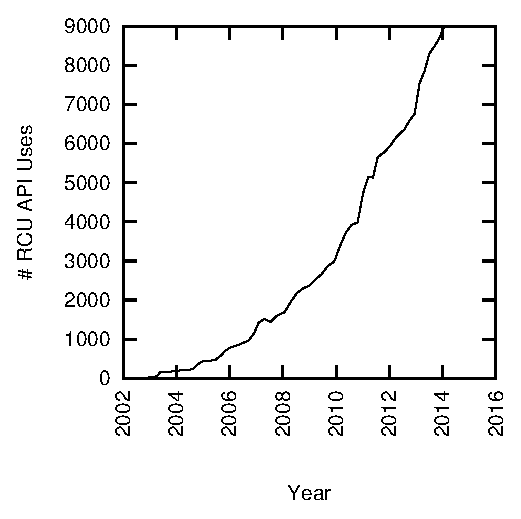
\includegraphics{appendix/rcuhist/linux-RCU}}
\caption{RCU API Usage in the Linux Kernel}
\label{fig:app:rcuhist:RCU API Usage in the Linux Kernel}
\end{figure}

\begin{figure}[bp]
\centering
\resizebox{3in}{!}{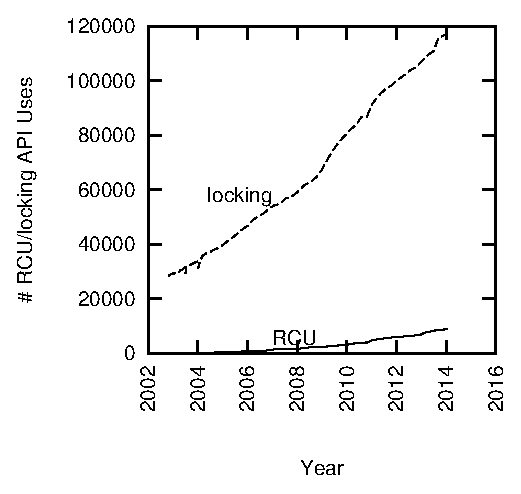
\includegraphics{appendix/rcuhist/linux-RCUlock}}
\caption{RCU API Usage in the Linux Kernel vs. Locking}
\label{fig:app:rcuhist:RCU API Usage in the Linux Kernel vs. Locking}
\end{figure}

\begin{figure}[tbp]
\centering
\resizebox{3in}{!}{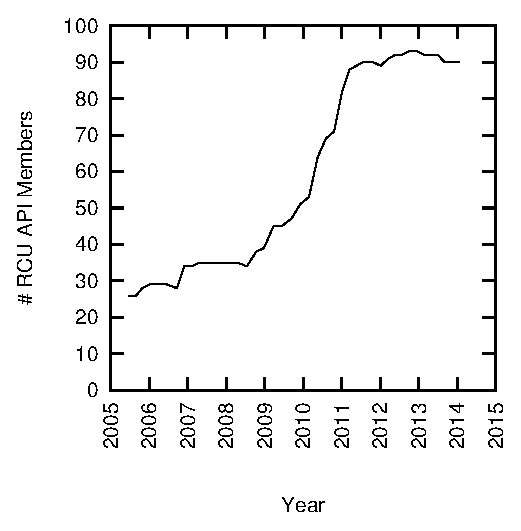
\includegraphics{appendix/rcuhist/rcuAPI}}
\caption{RCU API Growth Over Time}
\label{fig:app:rcuhist:RCU API Growth Over Time}
\end{figure}

리눅스 커널의 RCU 사용은
Figure~\ref{fig:app:rcuhist:RCU API Usage in the Linux Kernel}~\cite{PaulEMcKenneyRCUusagePage}
를 통해 볼 수 있듯이 시간에 따라 증가되었습니다.
RCU 는 코드 내에 존재하는 다른 동기화 메커니즘 (예를 들면, 네트워킹 프로토콜
스택의 \co{brlock}~\cite{Molnar00a,Torvalds2.5.69,Torvalds2.5.70}) 들을
대체했으며, 새로운 기능을 구현하는 코드 (예를 들면,
SELinux~\cite{JamesMorris04b} 에서의 audit 시스템) 와 함께 나타나기도 했습니다.
하지만, RCU 는
Figure~\ref{fig:app:rcuhist:RCU API Usage in the Linux Kernel vs. Locking} 에
보여지듯이 락킹에 비해서 틈새에만 사용되는 기술로 남아있습니다.
락킹이 커널 해커의 동시성 도구상자의 망치라면, RCU 는 아마도
스크류드라이버입니다.
만약 그렇다면,
Figure~\ref{fig:app:rcuhist:RCU API Growth Over Time} 를 통해 볼 수 있듯 매우
급격히 성장하는 스크류드라이버입니다.
\iffalse

The Linux kernel's usage of RCU has increased over the years,
as can be seen from
Figure~\ref{fig:app:rcuhist:RCU API Usage in the Linux Kernel}~\cite{PaulEMcKenneyRCUusagePage}.
RCU has replaced other synchronization mechanisms
in existing code
(for example, \co{brlock} in the networking protocol
stacks~\cite{Molnar00a,Torvalds2.5.69,Torvalds2.5.70}),
and it has also been introduced with code implementing
new functionality
(for example, the audit system within SELinux~\cite{JamesMorris04b}).
However, RCU remains a niche technology compared to locking,
as shown in
Figure~\ref{fig:app:rcuhist:RCU API Usage in the Linux Kernel vs. Locking}.
If locking is the hammer in the kernel hacker's concurrency toolbox,
perhaps RCU is the screwdriver.
If so, it is an rapidly evolving screwdriver, as can be seen in
Figure~\ref{fig:app:rcuhist:RCU API Growth Over Time}.
\fi

\section{RCU Evolution}
\label{sec:app:rcuhist:RCU Evolution}

이 섹션은 2008년 중반 이후 계속 진행중인 RCU 에 대한 경험을 제공합니다.
\iffalse

This section presents ongoing experience with RCU since mid-2008.
\fi

\subsection{2.6.27 Linux Kernel}

This release added the
\co{call_rcu_sched()},
\co{rcu_barrier_sched()}, and
\co{rcu_barrier_bh()} RCU API members.

\subsection{2.6.28 Linux Kernel}

RCU API 의 크기를 실제로 줄이는데에 관련된 변경사항으로
\co{list_for_each_rcu()} 기능의 제거가 있었습니다.
이 기능은 \co{list_head} 구조체를 구성하는 포인터쌍을 따라가기보다는 (헷갈릴 수
있지만, 리스트 헤더뿐 아니라 리스트 원소로 동작하는) 구조체들을 따라가는 장점을
가진 \co{list_for_each_entry_rcu()} 로 대체되었습니다.
이 변경은 2.6.28 리눅스 커널에 받아들여졌습니다.

안타깝게도, 2.6.28 리눅스 커널은 또한 \co{rcu_read_lock_sched()} 와
\co{rcu_read_unlock_sched()} RCU API 멤버들을 추가했습니다.
이 API 들은 가독성을 올리기 위해 추가되었습니다.
과거에는, \co{synchronize_sched()} 에 연관된 RCU read-side 크리티컬 섹션들을
표시하기 위해 인터럽트나 preemption 을 불능화 시키는데 사용되는 기능들을
사용했습니다.
하지만, 이는 개발자들이 preemption 이나 인터럽트를 불능화 시킬 필요가
없어졌지만 RCU 보호를 위한 필요를 알지 못할 때에 버그가 생기도록 이끌었습니다.
\co{rcu_read_lock_sched()} 의 사용은 그런 버그를 예방하는데 도움이 될 것입니다.
\iffalse

One welcome change involved an actual reduction in the size of RCU's
API with the removal of the \co{list_for_each_rcu()} primitive.
This primitive is superseded by \co{list_for_each_entry_rcu()},
which has the advantage of iterating over structures rather than
iterating over the pointer pairs making up a \co{list_head}
structure (which, confusingly, acts as a list element as well
as a list header).
This change was accepted into the 2.6.28 Linux kernel.

Unfortunately, the 2.6.28 Linux kernel also added
\co{rcu_read_lock_sched()} and
\co{rcu_read_unlock_sched()} RCU API members.
These APIs were added to promote readability.
In the past, primitives to disable interrupts or preemption were used
to mark the RCU read-side critical sections corresponding to
\co{synchronize_sched()}.
However, this practice led to bugs when developers removed the need
to disable preemption or interrupts, but failed to notice the need
for RCU protection.
Use of \co{rcu_read_lock_sched()} will help prevent such bugs in the
future.
\fi

\subsection{2.6.29 Linux Kernel}

새로운 더욱 확장성 있는 구현, ``Tree RCU'' 가 bitmap 을 combining tree 로
대체하면서 2.6.29 리눅스 커널에 받아들여졌습니다.
이 구현은 근래의 멀티프로세서들의 계속해서 증가하는 코어의 갯수에서 영감을
받아서 수백개의 CPU 환경을 위해 설계되었습니다.
현재의 구조상의 한계는 262,144 개 CPU 인데, 이는 개발자들이 (순진한 것일 수도
있지만) 한동안은 충분할 것이라 믿는 숫자입니다.
이 구현은 또한 preemptible RCU 의 개선된 dynamic-tick 인터페이스 인터페이스를
받아들였습니다.
\iffalse

A new more-scalable implementation, dubbed ``Tree RCU'', replaces
the flat bitmap with a combining tree, and was accepted into the 2.6.29
Linux kernel.
This implementation was inspired by the ever-growing core counts of
modern multiprocessors, and is designed for many hundreds of CPUs.
Its current architectural limit is 262,144 CPUs, which the developer
(perhaps na\"ively) believes to be sufficient for quite some time.
This implementation also adopts preemptible RCU's improved dynamic-tick
interface.
\fi

Mathieu Desnoyers 는 리눅스 커널의 tracing code 가 RCU 를 사용하도록 하는데
필요한 \co{rcu_read_lock_sched_notrace()} 와
\co{rcu_read_unlock_sched_notrace()} 를 추가했습니다.
이 API 들 없이는, RCU read-side 크리티컬 섹션을 추적하려는 시도는 무한 재귀
문제를 일으킵니다.
\iffalse

Mathieu Desnoyers added
\co{rcu_read_lock_sched_notrace()} and
\co{rcu_read_unlock_sched_notrace()},
which are required to permit the tracing code in the Linux kernel
to use RCU.
Without these APIs, attempts to trace RCU read-side critical sections
lead to infinite recursion.
\fi

Eric Dumazet 은 리스트 포인터에 단일 비트 마커들이 저장될 수 있도록 하는 새로운
종류의 RCU 로 보호되는 리스트를 추가했습니다.
이 종류의 리스트는 여러개의 락이 없는 알고리즘들을 가능하게 하는데, Maged
Michael 에 의해 보고된 것~\cite{MagedMichael04a} 등을 포함합니다.
Eric 의 작업은 \co{hlist_nulls_add_head_rcu()}, \co{hlist_nulls_del_rcu()},
\co{hlist_nulls_del_init_rcu()}, 그리고 \co{hlist_nulls_for_each_entry_rcu()}
를 추가합니다.
이는 또한 \co{hlist_nulls_node} 라는 이름의 새로운 구조체를 추가합니다.

또한, 이건 엄격히 말해서 리눅스 커널의 부분은 아니긴 하지만, 동시에 Mathieu
Desnoyers 는 그의 유저스페이스 RCU 구현~\cite{MathieuDesnoyers2009URCU} 을
발표했습니다.
이는 real-time user-level RCU 구현을 향한 중요한 첫걸음입니다.
\iffalse

Eric Dumazet added a new type of RCU-protected list that allows single-bit
markers to be stored in the list pointers.
This type of list enables a number of lockless algorithms, including
some reported on by Maged Michael~\cite{MagedMichael04a}.
Eric's work adds the \co{hlist_nulls_add_head_rcu()},
\co{hlist_nulls_del_rcu()}, \co{hlist_nulls_del_init_rcu()}, and
\co{hlist_nulls_for_each_entry_rcu()}.
It also adds a new structure named \co{hlist_nulls_node}.

Although it is strictly speaking not part of the Linux kernel, 
at about this same time, Mathieu Desnoyers announced his user-space
RCU implementation~\cite{MathieuDesnoyers2009URCU}.
This is an important first step towards a real-time user-level RCU
implementation.
\fi

\subsection{2.6.31 Linux Kernel}

Jiri Pirko 는 RCU-subscription 기능인 \co{rcu_dereference()} 를 더 높은 수준의
리스트 접근 기능에 포함시킨 \co{list_entry_rcu} 와 \co{list_first_entry_rcu()}
기능을 추가했는데, 이 기능들은 일련의 버그들을 제거해줄 수 있을 겁니다.

또한, ``Tree RCU'' 구현은 ``experimental'' 상태로부터 업그레이드 되었습니다.
\iffalse

Jiri Pirko added \co{list_entry_rcu} and \co{list_first_entry_rcu()}
primitives that encapsulate the \co{rcu_dereference()} RCU-subscription
primitive into higher-level list-access primitives, which will hopefully
eliminate a class of bugs.

In addition, the ``Tree RCU'' implementation was upgraded from
``experimental'' status.
\fi

\subsection{2.6.32 Linux Kernel}

리눅스 커널의 이 버전에서의 가장 큰 변경은 ``Classic RCU'' 구현의 제거일
것입니다.
이 구현은 ``Tree RCU'' 구현으로 대체되었습니다.

이 버전은 그 외에도 여러 변경을 가졌는데, 다음과 같은 것들이 포함됩니다:
\iffalse

Perhaps the largest change in this version of the Linux kernel
is the removal of the old ``Classic RCU'' implementation.
This implementation is superseded by the ``Tree RCU'' implementation.

This version saw a number of other changes, including:
\fi

\begin{enumerate}
\item	\co{synchronize_rcu_expedited()}, \co{synchronize_sched_expedited()},
	그리고 \co{synchronize_rcu_bh_expedited()} RCU API 멤버들의 추가.
	이 기능들은 grace period 를 신속히 처리하기 위해 측정을 한다는 점을
	제외하고는 non-expedited 버전의 것들과 동일합니다.
\item	``Tree RCU'' 구현에 preemptible-RCU 기능들을 추가함으로써 리눅스로
	돌아가는 커다란 멀티프로세서 머신에서의 real-time response 에 대한
	문제를 해결.
\item	이 새로운 ``Tree Preemptible RCU'' 구현은 기존의 preemptible RCU 구현을
	구형으로 만들어서 리눅스 커널에서 사라지게 했습니다.
\iffalse

\item	The appearance of \co{synchronize_rcu_expedited()},
	\co{synchronize_sched_expedited()}, and
	\co{synchronize_rcu_bh_expedited()} RCU API members.
	These primitives are equivalent to their non-expedited
	counterparts, except that they take measures to expedite the
	grace period.
\item	Add preemptible-RCU functionality to the ``Tree RCU''
	implementation, thus removing one obstacle to real-time
	response from large multiprocessor machines running Linux.
\item	This new ``Tree Preemptible RCU'' implementation obsoletes
	the old preemptible RCU implementation, which was removed
	from the Linux kernel.
\fi
\end{enumerate}

\subsection{2.6.33 Linux Kernel}

이 릴리즈에서의 가장 극적인 추가사항은 Tree RCU 에서의 day-one
버그~\cite{PaulEMcKenney2009HuntingHeisenbugs} 였을 겁니다.
다른 변경 사항들은 다음과 같습니다:
\iffalse

Perhaps the most dramatic addition to this release was
a day-one bug in Tree RCU~\cite{PaulEMcKenney2009HuntingHeisenbugs}.
Other changes include:
\fi

\begin{enumerate}
\item	``RCU: The Bloatwatch
	Edition''~\cite{PaulEMcKenney2009LWNBloatWatchRCU} 라고도 알려진 ``Tiny
	RCU''.
\item	\co{synchronize_srcu_expedited()} 의 형태의 expedited SRCU.
\item	앞서 이야기된 버그에 의해 촉발된 Tree RCU 동기화의 정리.
\item	Tree Preemptible RCU 의 expedited 구현의 추가 (이전의 릴리즈에서,
	``expedited'' 지원은 단순히 \co{synchronize_rcu()} 로 매핑되었는데,
	이는 의미적으로는 옳은 동작이지만 성능 관점에서는 별로 도움이 되지
	않았습니다.)
\item	스트레스 테스트를 향상시킨 네번째 수준의 Tree RCU 추가.
	이로 인해, 누군가가 16,777,216 개의 CPU 를 가진 시스템에서 리눅스를
	돌리고자 한다면, RCU 를 그런 환경에도 준비가 되었습니다!
	대략 1600 만개의 per-CPU 데이터 원소들을 스캐닝 하는 것에 대한 응답시간
	의미 \ldots
\iffalse

\item	``Tiny RCU'', also known as ``RCU: The Bloatwatch
	Edition''~\cite{PaulEMcKenney2009LWNBloatWatchRCU}.
\item	Expedited SRCU in the form of
	\co{synchronize_srcu_expedited()}.
\item	A cleanup of Tree RCU synchronization prompted by the
	afore-mentioned bug.
\item	Add expedited implementation for Tree Preemptible RCU
	(in earlier releases, ``expedited'' support had simply
	mapped to \co{synchronize_rcu()}, which is semantically
	correct if somewhat unhelpful from a performance viewpoint.)
\item	Add a fourth level to Tree RCU, which improves stress testing.
	Therefore, if someone ever wants to run Linux on a system with
	16,777,216 CPUs, RCU is ready for them!
	Give or take the response-time implications of scanning
	through 16 million per-CPU data elements \ldots
\fi
\end{enumerate}

\subsection{2.6.34 Linux Kernel}

이 릴리즈에서 가장 눈에 띄는 추가사항은 \co{rcu_dereference()} 가 올바른 락킹
조건을 체크하도록 하는 \co{CONFIG_PROVE_RCU}~\cite{PaulEMcKenney2010LockdepRCU}
였습니다.
다른 변경들은 다음과 같습니다:
\iffalse

The most visible addition for this release was \co{CONFIG_PROVE_RCU},
which allows \co{rcu_dereference()} to check for correct locking
conditions~\cite{PaulEMcKenney2010LockdepRCU}.
Other changes include:
\fi

\begin{enumerate}
\item	기존 grace period 를 강제하고 새로운 grace period 를 시작하는 사이의
	Tree RCU 의 상호작용의 간소화.
\item	Free-running 카운터들이 부호 없게 되도록 카운터들을 재작업.
	(C-컴파일러 해커들이 부호 있는 정수를 오버플로우 시킴으로써 코드를
	깨먹을 수 있는 최적화를 이야기 하면서 얼굴에 띄웠던 즐거운 표정을
	여러분은 상상하지도 못할겁니다!!!)
\item	RCU read-side 크리티컬 섹션 안에서 지나치게 많은 시간 동안 preemption
	당한 모든 태스크들을 출력하기 위한 Tree Preemptible RCU 의 stall 파악
	기능 업데이트.
\item	Tree RCU 의 CPU-stall-detection 코드의 다른 버그 수정과 개선.
	이 코드는, 예를 들어, 인터럽트가 불능화 된채 무한루프를 돌거나 하는,
	락업된 CPU 들을 체크합니다.
\item	배터리로 동작하는 멀티프로세서 시스템에서 마지막 CPU 가 idle 상태로
	빠질 때 grace period 를 가속화 시키기 위한 일부 코드를 프로토타입.
	시스템이 모든 CPU 들이 꺼질 수 있는 상태로 넘어가는데에 추가적인 몇
	밀리세컨드를 RCU 가 가져가는데에 대해서 상당히 불쾌해 했던 사람들이
	존재합니다!
\iffalse

\item	Simplifying Tree RCU's interactions between
	forcing an old grace period and starting a new one.
\item	Rework counters so that free-running counters are unsigned.
	(You simply cannot imagine the glee on the faces of certain
	C-compiler hackers while they discussed optimizations that would
	break code that naively overflowed signed integers!!!)
\item	Update Tree Preemptible RCU's stall detection to print out
	any tasks preempted for excessive time periods while in
	an RCU read-side critical section.
\item	Other bug fixes and improvements to Tree RCU's CPU-stall-detection
	code.
	This code checks for CPUs being locked up, for example,
	in infinite loops with interrupts disabled.
\item	Prototype some code to accelerate grace periods when the
	last CPU goes idle in battery-powered multiprocessor
	systems.
	There were people who were quite unhappy about RCU taking
	a few extra milliseconds to get the system in a state
	where all CPUs could be powered down!
\fi
\end{enumerate}

\subsection{2.6.35 Linux Kernel}

이 릴리즈는 여러개의 버그 수정과 코드 정리를 추가합니다.
여기서의 주요 변경 사항은 Mathieu Desnoyers 의 RCU 콜백의 오용을 위한 검사로,
예를 들면 하나의 grace period 안에서 \co{rcu_head} 구조체를 \co{call_rcu()} 에
두번 보내거나 하는 경우입니다.
\iffalse

This release includes a number of bug fixes and cleanups.
The major change is the first installment of Mathieu Desnoyers's
patch to check for misuse of RCU callbacks, for example, passing
a \co{rcu_head} structure to \co{call_rcu()} a second time within
a single grace period.
\fi

\subsection{2.6.36 Linux Kernel}

Mathieu Desnoyers 의 디버그 목적의 작업물의 핵심은 2.6.36 에 나타났는데, 일부
코드 정리 작업은 다른 maintainer 트리들에 나오는 커밋들과의 종속성 때문에
2.6.37 로 미뤄졌습니다.
Arnd Bergmann 의 sparse RCU 검사의 한 핵심적 부분이 2.6.36 에 나타났는데,
나머지는 역시 다른 maintainer 트리에 나오는 커밋과의 종속성 때문에 2.6.37 로
미뤄졌습니다.
마지막으로, Eric Dumazet 으로부터의 패치는 \co{rcu_dereference_bh()} 의 에러
검사에서의 에러를 고쳤습니다.
\iffalse

The core of Mathieu Desnoyers's debugobjects work appeared in 2.6.36,
with some cleanups deferred to 2.6.37 due to dependencies on commits
flowing up other maintainer trees.
A key piece of Arnd Bergmann's sparse RCU checking appeared in 2.6.36,
with the remainder deferred to 2.6.37, again due to dependencies on
commits flowing up other maintainer trees.
Finally, a patch from Eric Dumazet fixed an error in
\co{rcu_dereference_bh()}'s error checking.
\fi

\subsection{2.6.37 Linux Kernel}

Mathieu Desnoyers 의 디버그 목적 작업의 마지막 정리 작업이 2.6.37 에 Arnd
Bergmann 의 sparse 기반 검사 작업과 함께 나타났습니다.
Lai Jiangshan 은 rcutorture 에 preemption 에 의한 문제 상황을 추가했고 Tree RCU
의 per-CPU 데이터 처리를 일부 간단화 시켰습니다.
Tetsuo Handa 는 RCU lockdep 으로 나온 문제 하나를 고쳤고, Christian Dietrich 는
불필요하게 반복된 \co{#ifdef} 를 제거했으며, Dongdong Deng 은 일부 Tree RCU
제어 데이터로의 락 없는 액세스를 가능하게 하도록 \co{ACCESS_ONCE()} 를
추가했습니다.

Paul 의 preemptible Tiny RCU 의 구현 또한 RCU CPU stall-warning 코드, docbook
수정, 중복 코드의 합체, Tree RCU 속도향상, RCU callback flow 에의 queuing 모델
지원에 대한 tracing 추가, 그리고 몇가지 기타 수정과 정리 작업과 함께 2.6.37
에서 나타났습니다.
\iffalse

The final cleanups from Mathieu Desnoyers's debugobjects work appeared
in 2.6.37, as did the remainder of Arnd Bergmann's sparse-based checking work.
Lai Jiangshan added some preemption nastiness to rcutorture and
made some simplifications to Tree RCU's handling of per-CPU data.
Tetsuo Handa fixed an RCU lockdep splat, Christian Dietrich removed
a redundant \co{#ifdef}, and Dongdong Deng added an
\co{ACCESS_ONCE()} that help call out lockless accesses to some
Tree RCU control data.

Paul's implementation of preemptible Tiny RCU also appeared in
2.6.37, as did a number of enhancements to the RCU CPU stall-warning
code, docbook fixes, coalescing of duplicate code, Tree RCU speedups,
added tracing to support queuing models on RCU callback flow,
and several miscellaneous fixes and cleanups.
\fi

\subsection{2.6.38 Linux Kernel}

Lai Jiangshan 은 \co{synchronize_sched_expedited()} 를 \co{kernel/sched.c} 에서
그것이 유래한 \co{kernel/rcutree.c} 와 \co{kernel/rcu_tiny.c} 로 옮겼습니다.
그는 또한 \co{orphan_cbs_list} 를 제거함으로써 CPU-hotplug 오퍼레이션 동안의
RCU-callback 처리를 단순화 해서, offline 이 되는 CPU 에 의해 고아가 되는 RCU
콜백들이 곧바로 해당 offline 화 시키는 동작을 함께 돕는 CPU 들에 의해 곧바로
처리될 수 있도록 했습니다.
Tejun Heo 는 \co{synchronize_sched_expedited()} 의 batching 기능을 개선했는데,
이는 결국 많은 동시적 \co{synchronize_sched_expedited} 오퍼레이션들을 갖는
워크로드들의 성능과 확장성을 개선했습니다.
Fre\'ed\'eric Weisbecker 는 RCU 를 idle 상태일 때 더욱 전력에 효율적이도록
만들어주는 RCU 핵심 코드상의 일부 변경을 제공했습니다.
Mariusz Kozlowski 는 \co{__list_for_each_rcu()} 상의 문법상 에러를 고쳐졌고, 곧
사라졌습니다.
(하지만 이 고쳐진 버전은 필요한 경우를 위해 git tree 상에 존재합니다.)
Nick Piggin 은 RCU 로 보호되는 bit-locked doubly-linked list 들을 위해
\co{hlist_bl_set_first_rcu()},
\co{hlist_bl_first_rcu()},
\co{hlist_bl_del_init_rcu()},
\co{hlist_bl_del_rcu()},
\co{hlist_bl_add_head_rcu()}, 그리고
\co{hlist_bl_for_each_entry_rcu()} 기능을 추가했습니다.
Christoph Lameter 는 변수가 곧바로 접근되는 경우에 사용되기 위한
\co{__get_cpu_var()} 의 최적화된 변종인 \co{__this_cpu_read()} 를 구현했습니다.
\iffalse

Lai Jiangshan moved \co{synchronize_sched_expedited()} out of
\co{kernel/sched.c} and into \co{kernel/rcutree.c} and
\co{kernel/rcu_tiny.c} where it belongs.
He also simplified RCU-callback handling during CPU-hotplug operations
by eliminating the \co{orphan_cbs_list}, so that RCU callbacks
orphaned by a CPU that is going offline are immediately adopted by
the CPU that is orchestrating the offlining sequence.
Tejun Heo improved \co{synchronize_sched_expedited()}'s batching
capabilities, which in turn improves performance and scalability
for workloads with many concurrent \co{synchronize_sched_expedited}
operations.
Fr\'ed\'eric Weisbecker provided a couple of subtle changes to the
RCU core code that make RCU more power-efficient when idle.
Mariusz Kozlowski fixed an embarrassing syntax error in
\co{__list_for_each_rcu()}, which was then removed.
(But the fixed version is there in the git tree should it be needed.)
Nick Piggin added the \co{hlist_bl_set_first_rcu()},
\co{hlist_bl_first_rcu()},
\co{hlist_bl_del_init_rcu()},
\co{hlist_bl_del_rcu()},
\co{hlist_bl_add_head_rcu()}, and
\co{hlist_bl_for_each_entry_rcu()} primitives for RCU-protected use
of bit-locked doubly-linked lists.
Christoph Lameter implemented \co{__this_cpu_read()}, which is an
optimized variant of
\co{__get_cpu_var()} for use in cases where the variable is accessed directly.
\fi

또한, \co{TINY_RCU} 는 priority boosting 을 얻었고,
\co{synchronize_srcu_expedited()} 의 race condition 이 고쳐졌고,
\co{synchronized_srcu_expedited()} 가 동시적인 읽기 쓰레드들이 존재할 때에
expedited 본성을 얻을 수 있도록 수정되었으며, grace-period 시작/종료 검사가
개선되었고, \co{TREE_RCU} 의 leaf-level fanout 이 lock-contention 문제들을
고치기 위해 16 으로 제한되었습니다.
이 마지막 변경은 \co{TREE_RCU} 와 \co{TREE_PREEMPT_RCU} 가 지원할 수 있는 CPU
들의 최대 갯수를 4,194,304 로 줄였는데, 이는 (다시 말하지만, 어쩌면 순진하게도)
충분할 것으로 여겨집니다.
\iffalse

In addition, \co{TINY_RCU} gained priority boosting, a race condition
in \co{synchronize_sched_expedited()} was fixed,
\co{synchronize_srcu_expedited()} was modified to retain its expedited
nature in the face of concurrent readers,
grace-period begin/end checks were improved,
and the \co{TREE_RCU} leaf-level fanout was limited to 16 in order to fix
lock-contention problems.
This last change reduces the maximum number of CPUs that \co{TREE_RCU}
and \co{TREE_PREEMPT_RCU} can support down to 4,194,304, which is
(again, perhaps na\"ively) believed to be sufficient.
\fi

\subsection{2.6.39 Linux Kernel}

Lai Jiangshan 은 task 가 RCU read-side 크리티컬 섹션 내에서 종료되는 경우에
디버깅 상태를 보존하기 위해 \co{exit_rcu()} 가 \co{rcu_read_unlock()} 대신
\co{__rcu_read_unlock()} 을 호출하도록 만들었으며, Jesper Juhl 은 rcutorture
내의 중복된 \co{sched.h} 포함을 제거했고, Amerigo Wang 은 \co{rcu_fixup_free()}
로부터 의미없는 코드들을 일부 제거했습니다.

또한, MCE 서브시스템에서의 사용을 위해 새로운 \co{rcu_access_index()} 가
만들어졌습니다.
\iffalse

Lai Jiangshan made \co{TINY_RCU}'s \co{exit_rcu()} invoke
\co{__rcu_read_unlock()}
rather than \co{rcu_read_unlock()} in case of a task exiting while
in an RCU read-side critical section in order to preserve debugging
state,
Jesper Juhl removed a duplicate include of \co{sched.h} from
rcutorture,
and
Amerigo Wang removed some dead code from \co{rcu_fixup_free()}.

In addition, a new \co{rcu_access_index()} was created for use in the
MCE subsystem.
\fi

\subsection{3.0 Linux Kernel}

많은 사람들이 2.6.40 릴리즈가 될 것이라 예상했던 것은 3.0 릴리즈가 되었습니다.
여기서 가장 중요한 RCU 기능은 Tree RCU 를 위한 priority boosting 의
추가였습니다: 계획됐던 것보다 여러면에서
중요해서~\cite{PaulEMcKenney2011RCU3.0trainwreck}, 3.0-rc7 뒤의 RCU 수정이
되었습니다.
Shaohua Li, Peter Zijlstra, Steven Rostedt 의 RCU, 스케쥴러, 그리고 thread 로
돌아가는 인터럽트들 사이의 충돌의 fallout 처리에 대한 많은 도움에 감사를 드리는
바입니다.
또한, RCU CPU stall warning 들은, 여전히 커널 부트 패러미터나 \co{sysfs} 로
조정될 수 있는 \co{rcu_cpu_stall_suppress} 모듈 패러미터로 불능화 될 수 있긴
하지만, 이제 무조건적으로 Tree RCU 안으로 컴파일 됩니다.
\iffalse

What many expected to be the 2.6.40 release became instead the 3.0 release.
The most important RCU feature was the addition of priority boosting
for Tree RCU: Important in more ways than
planned~\cite{PaulEMcKenney2011RCU3.0trainwreck}, resulting in RCU
fixes after 3.0-rc7.
Kudos to Shaohua Li, Peter Zijlstra, Steven Rostedt for much help
dealing with the fallout of the collision between RCU, the scheduler,
and threaded interrupts.
In addition, RCU CPU stall warnings are now unconditionally compiled
into Tree RCU, though they may still be disabled via the
\co{rcu_cpu_stall_suppress} module parameter, which may be controlled
from either the kernel boot parameter string or \co{sysfs}.
\fi

Mathieu Desnoyers 는 non-preemptible RCU 구현에 들어오게 되는
\co{DEBUG_OBJECTS_RCU_HEAD} 체크를 활성화 시켰습니다.
Lai Jiangshan 은 fire-and-forget \co{kfree_rcu()} 를 만들었고 (그리고 이를
커널을 통해 적용했습니다), 또한 \co{exit_rcu()} 가 task 가 RCU read-side
크리티컬 섹션 내에서 끝나는 경우에 디버깅 상태를 유지할 수 있도록 하기 위해
\co{rcu_read_unlock()} 대신 \co{__rcu_read_unlock()} 을 호출하도록
만들었습니다.
Eric Dumazet 는 더 나아가서 \co{TINY_RCU} 를 감소시켰고 Gleb Natapov 는
가상화가 guest OS 와의 문맥 전환 시에 일어나는 quiescent state 들 사이에 RCU 가
신경을 쓸 수 있도록 RCU hook 들을 추가했습니다.
Peter Zijlstra 는 RCU kthread 블록킹과 wakeup 을 streamline 시켰습니다.
\iffalse

Mathieu Desnoyers enabled \co{DEBUG_OBJECTS_RCU_HEAD} checking to
be carried out in non-preemptible RCU implementations.
Lai Jiangshan created a fire-and-forget \co{kfree_rcu()} (and applied
it throughout the kernel),
and also made \co{TREE_RCU}'s \co{exit_rcu()} invoke
\co{__rcu_read_unlock()}
rather than \co{rcu_read_unlock()} in case of a task exiting while
in an RCU read-side critical section in order to preserve debugging
state.
Eric Dumazet further shrank \co{TINY_RCU} and
Gleb Natapov added RCU hooks to allow virtualization to call RCU's
attention to quiescent states that occur when switching context to
and from a guest OS.
Peter Zijlstra streamlined RCU kthread blocking and wakeup.
\fi

\subsection{3.1 Linux Kernel}

3.1 버전은 Arun Sharma, Jiri Kosina, Michal Hocko, Peter Zijlstra, 그리고 Jan
H. Sch\"{o}nherr 로부터의 마이너한 수정들과 코드 정리들을 포함한, RCU 에
있어서는 조용한 시간이었습니다.
\iffalse

The 3.1 version was a quiet time for RCU, with cleanups and minor fixes
from Arun Sharma, Jiri Kosina, Michal Hocko, Peter Zijlstra,
and Jan H. Sch\"{o}nherr.
\fi

\subsection{3.2 Linux Kernel}

3.2 리눅스 커널은 RCU 의 코드의 꼭대기부터 바닥까지의 검사 첫번째 단계에서
발견된 문제들에 대한 여러 수정사항들을 담고 있습니다.
이 검사의 결과물 가운데 하나는 코드의 irq 불능화된 구간이 preemptible RCU
read-side 크리티컬 섹션의 시작이 아니라 끝과 겹치게 되면 데드락이 일어날 수
있다는 것이었습니다.
따라서, 부분적으로 irq 불능화된 코드 구간과 겹칠 수 있는 RCU read-side 크리티컬
섹션들을 만들지 마세요:
대신에, irq 불능화된 코드 섹션을 주어진 RCU read-side 크리티컬 섹션 안에 완전히
집어넣거나 그 반대로 하거나 하세요.
\iffalse

The 3.2 Linux kernel contains a number of fixes to issues located
during the first phase of a top-to-bottom inspection of RCU's code.
One outcome of this inspection is that deadlock can occur if
an irq-disabled section of code overlaps the end but not the beginning
of a preemptible RCU read-side critical section.
Therefore, do not code RCU read-side critical sections that partially
overlap with irq-disabled code sections:
Instead, either fully enclose the irq-disable code sections within a
given RCU read-side critical section or vice versa.
\fi

이 릴리즈는 RCU 이벤트 추적 기능을 처음으로 보였습니다.
Eric Dumazet 는 RCU 의 kthread 들이 NUMA 시스템에 최적화된 방식으로 위치된
메모리를 가지게 됨을 보장하는 \co{kthread_create_on_node()} 기능을
적용했습니다.
그는 또한 \co{rcu_assign_pointer()} 가 무조건적으로 메모리 배리어를 삽입하도록
했는데, 특정 환경에서는 이 메모리 배리어가 생략되게 했던 기존의 컴파일러의
마술이 그보다 최신의 버전의 컴파일러에서는 통하지 않았기 때문입니다.
따라서, RCU 로 보호되는 포인터에 \co{NULL} 을 할당할 때에는,
\co{rcu_assign_pointer()} 보다는 \co{RCU_INIT_POIINTER()} 를 사용하세요.
\iffalse

This release saw the first RCU event-tracing capabilities.
Eric Dumazet applied the new
\co{kthread_create_on_node()} primitive to ensure that RCU's
kthreads have memory placed optimally on NUMA systems.
He also
made the \co{rcu_assign_pointer()} unconditionally insert a
memory barrier because the earlier compiler magic permitting this
barrier to be omitted under certain circumstances fails in newer
versions of the compiler.
Therefore, when assigning \co{NULL} to an RCU-protected pointer,
use \co{RCU_INIT_POINTER()} rather than \co{rcu_assign_pointer()}.
\fi

Shaohua Li 는 RCU 의 per-CPU kthread 들의 불필요한 self-wakeup 을 제거했고,
Andi Kleen 은 일부 충돌되는 변수 선언들을 정리했습니다.
Mike Galbraith 는 RCU 가 \co{RCU_BOOST_PRIO} 커널 패러미터를 무시하게 하는
버그를 잡았고, 마지막으로, 계속해서 확장되는 RCU 의 기능들을 잡을 수 있도록
rcutorture 가 진척을 만들었습니다.
\iffalse

Shaohua Li eliminated an unnecessary self-wakeup of RCU's per-CPU
kthreads, and Andi Kleen cleaned up some conflicting variable
declarations.
Mike Galbraith fixed a bug that caused RCU to ignore the
\co{RCU_BOOST_PRIO} kernel parameter, and finally,
rcutorture made some headway in catching up to the ever-expanding
RCU capabilities.
\fi

\subsection{3.3 Linux Kernel}

3.3 리눅스 커널은 RCU 의 idle CPU 가 아니라면 scheduling-clock ticks 를 위한
필요를 줄여주는 에너지 효율성 개선, uprobes 에 의해 필요시되는 새로운
\co{srcu_read_lock_raw()} 기능, 여전히 진행중인 RCU 전체 검사로 찾아내어진
문제들에 대한 수정사항들, 그리고 스크립트로 짜여진, 타입이나 userspace
레이아웃의 존재에 의존적이지 않은 KVM 기반의 RCU 테스트를 가능하게 하는
\co{rcutorture} 개선사항이 포함되었습니다.

또한 Thomas Gleixner 로부터의 \co{-rt} RCU 패치들 포함했고, 또한 dyntick-idle
모드부터 usermode 수행까지의 응용을 지원하는 Fr\'ed\'eric Weisbecker 로부터의
RCU 기반시설 관련 여러 패치들을 포함했습니다.
\iffalse

The 3.3 Linux kernel contains
energy-efficiency improvements that reduce RCU's need for
scheduling-clock ticks from otherwise idle CPUs,
a new \co{srcu_read_lock_raw()} primitive needed by uprobes,
additional fixes for issues located in the still-ongoing top-to-bottom
inspection of RCU,
and improvements to \co{rcutorture} that enable scripted KVM-based
testing of RCU, independent of the type or presence of userspace layout.

Also included were some \co{-rt} RCU patches from Thomas Gleixner,
as well as
a number of RCU-infrastructure patches from Fr\'ed\'eric Weisbecker
in support of the long-hoped-for application of dyntick-idle mode
to usermode execution.
\fi

비록 일부 초기 작업들은 RCU-preempt 의 \co{__rcu_read_lock()} 과
\co{__rcu_read_unlock()} 가 inline 될 수 있도록 했지만, 그보다 훨씬 많은 작업이
다양한 inlcude 파일 문제들을 푸는데 필요했습니다.
마지막으로, Rusty Russell 로부터의 잡다한 수정들이 있었습니다.

\co{rcu_barrier_expedited()} 에 대한 초기 요청이 있었습니다만, 그 요청을 한
사람은 이 문제를 풀기 위한 다른 방법을 찾았기에, 이는 상대적으로 낮은
우선순위를 가졌습니다.
\iffalse

Although some initial work has gone into permitting RCU-preempt's
\co{__rcu_read_lock()} and \co{__rcu_read_unlock()} to be inlined,
much more work is needed to disentangle various include-file issues.
Finally, there were miscellaneous fixes from Rusty Russell.

There has been an initial request for \co{rcu_barrier_expedited()},
but given that the requester found another way to solve this problem,
this has relatively low priority.
\fi

\subsection{3.4 Linux Kernel}

3.4 커널은 전력 효율성을 위해 급격한 idle 진입/종료 워크로드에 대한 단점을
줄이는 작업을 포함했습니다.
여기서 관리된 트레이드오프는 긴 idle 시간에 대비해서 idle 진입에 대한 작업의
증가이고, 따라서 이 릴리즈에서의 변경사항들은 추가적인 노력이 의미없을 때를
인식하는 데 대해 더 나은 일을 하는데, 예를 들어 CPU 가 워크로드 때문에 idle 을
급격하게 진입했다가 빠져나간다면 CPU 가 더 오래 sleep 상태에 머무르게 하는
idle-entry 동작을 취하는데에 약간의 이점이 있습니다.
\iffalse

The 3.4 kernel contains yet more energy-efficiency work, reducing their
downsides to rapid idle entry/exit workloads.
The tradeoff managed here is increased work on idle entry compared to
longer idle times, and so the changes in this release do a better job of
recognizing when additional effort is futile, for example, if the
CPU is entering and exiting idle rapidly due to the workload, there is
little point in taking idle-entry actions that would allow the CPU to
stay asleep longer.
\fi

이 릴리즈는 또한 계속해서 증가하는 사용예인 idle CPU 들에서 RCU 를 호출하는
행위를 처리하는데 사용되기 위한 \co{RCU_NOIDLE()} 을 추가했습니다.
RCU 는 idle CPU 들을 무시하기 때문에, 이런 행위는 상당히 위험합니다.
따라서 이 새로운 \co{RCU_NONIDLE()} 매크로는 RCU read-side 크리티컬 섹션이 그
일을 할 수 있도록 idle 로부터 급격하게 빠져나가도록 합니다.

RCU 의 CPU hotplug 처리가 개선되었고, rcutorture 는 RCU CPU stall 경고를
테스트하기 위한 기본적 기능을 일부 얻었으며, 이 stall 경고 자체는 더 많은
정보를 추가하고 sysfs 를 통해 타임아웃을 제어할 수 있는 기능을 추가함으로써
개선되었습니다.
\co{TREE_RCU} 는 \co{CONFIG_SMP=n} 커널에서는 더이상 사용되지 않습니다;
\co{TINY_RCU} 가 그대신 사용됩니다.
이 릴리즈는 또한, non-preemptible-RCU read-side 크리티컬 섹션 내에서의 잠자는
행위와 RCU read-side 크리티컬 섹션 내에서의 idle loop 진입을 위한 lockdep-RCU
체크의 추가를 포함합니다.
\iffalse

This release also added \co{RCU_NONIDLE()}, which is used to handle
the increasingly frequent practice of invoking RCU from idle CPUs.
Because RCU ignores idle CPUs, this practice is quite dangerous.
The new \co{RCU_NONIDLE()} macro therefore carries out a momentary
exit from idle so that RCU read-side critical sections can do their job.

RCU's handling of CPU hotplug was improved, rcutorture gained some
primitive ability to test RCU CPU stalls warnings, and the stall
warnings themselves were improved by adding more information and
by adding the ability to control timeouts via sysfs.
\co{TREE_RCU} no longer may be used in \co{CONFIG_SMP=n} kernels;
\co{TINY_RCU} is used instead.
This release also saw the addition of lockdep-RCU checks for sleeping
in a non-preemptible-RCU read-side critical section, as well as for
entering the idle loop while in an RCU read-side critical section.
\fi

\co{TINY_RCU} 는 v3.0-rc7 RCU
trainwreck~\cite{PaulEMcKenney2011RCU3.0trainwreck} 을 위한 \co{TREE_RCU}
수정사항들을 상속받았습니다.
Grace-period 초기화 프로세스는 기존의 single-node 최적화를 제거했으며, offline
이 된 CPU 들에 남아있는 콜백들은 더이상 두번째의 grace period 전체를 거치지
않아도 되게 되었습니다.
더 나아가서, offline CPU 들은 더이상 RCU 콜백들을 호출할 수 없게 되었습니다.

이 외에도 더 많은 전력 효율성 코드의 수정사항들이 idle CPU 위에서 비참하게
살아있을 수도 있는 Time lazy 콜백들의 양을 제한했습니다.
마지막으로, Fr\'ed\'eric Weisbecker, Heiko Carstens, Julia Lawall, Hugh
Dickins, Jan Beulich, 그리고 Paul Gortmaker 에 의해서 다수의 수정사항들이
추가되었습니다.
\iffalse

\co{TINY_RCU} inherited the \co{TREE_RCU} fixes for the v3.0-rc7 RCU
trainwreck~\cite{PaulEMcKenney2011RCU3.0trainwreck}.
The grace-period initialization process dropped the old single-node
optimization, and callbacks remaining on offlined CPUs no longer
need to go through a second full grace period.
Furthermore, offline CPUs are no longer permitted to invoke RCU
callbacks.

Yet more tweaks to the energy-efficiency code limited the amount of
time lazy callbacks could languish on an idle CPU.
Finally, a number of fixes were supplied by Fr\'ed\'eric Weisbecker,
Heiko Carstens, Julia Lawall, Hugh Dickins, Jan Beulich, and Paul
Gortmaker.
\fi

\subsection{3.5 Linux Kernel}

3.5 리눅스 커널은 \co{CONFIG_RCU_FAST_NO_HZ} 전력 효율성 코드에 타이머 처리와
\co{RCU_NOIDLE()} 에 의한 idle 로부터의 정지에 대한 올바른 처리 등을 포함한, 더
많은 변화를 가져왔습니다.

이는 또한 \co{rcu_barrier()} 와 그 비슷한 것들에 의한 분열을 콜백들을 아무것도
갖지 않은 CPU 에 넣는 것을 막음으로써 줄였습니다.
이 작업은 또한 \co{rcu_barrier()} 와 offline 이 된 CPU 들에 의하 고아가 된
콜백들 사이의 상호작용을 보다 명시적이게 만들었는데, 이는 일부 교묘한 race
condition 들을 막는데에 필요했던 것입니다.
\co{__rcu_read_unlock()} 을 inline 하려다 실패한 시도는 그러나 RCU 의 task 종료
처리의 오버헤드를 줄이고 격리화 시키는 효과를 남겼습니다.

이 릴리즈는 Lai Jiangshan 에 의한 SRCU 의 완전한 재작성, 그 외에도 Jan
Engelhardt, Michel Machado, 그리고 Dave Jones 에 의한 수정사항들을
포함했습니다.
\iffalse

The 3.5 Linux kernel included yet more adjustments to the
\co{CONFIG_RCU_FAST_NO_HZ} energy-efficiency code, including timer
handling and proper handling of \co{RCU_NONIDLE()} pauses out of
idle.

It also included work to reduce the disruption due to \co{rcu_barrier()}
and friends by avoiding enqueuing callbacks on CPUs that have none.
This work also made the interaction between \co{rcu_barrier()} and
callbacks orphaned by offlined CPUs more explicit, which was required
in order to avoid some nasty race conditions.
An abortive attempt to inline \co{__rcu_read_unlock()} left but one
commit that consolidated and reduced the overhead of RCU's
task-exit handling.

This release contains a complete rewrite of SRCU by Lai Jiangshan as
well as fixes from Jan Engelhardt, Michel Machado, and Dave Jones.
\fi

\subsection{3.6 Linux Kernel}

3.6 리눅스 커널은 \co{rcu_node} 트리의 leaf 단계 fanout 을 boot-time 패러미터를
통해 제어 가능하게 함으로써 수천개의 CPU 들을 갖는 시스템에서의 RCU 의 스케쥴링
응답시간 효과를 줄이기 위한 변경 사항들 중 첫번째 것들을 포함했습니다.
이 변경은 grace-period 초기화 동안 만져져야 하는 메모리의 양을 4배 줄였고, 그로
인해 응답시간의 효과를 200 마이크로세컨드에서 60-70 마이크로세컨드로
줄였습니다.
이 릴리즈는 또한 \co{rcu_barrier()} 동시성을 증가시켰습니다.

전통을 따라서, 이 릴리즈는 또한 \co{CONFIG_RCU_FAST_NO_HZ} 기능을 위한 전력
효율성 상의 변경 사항을 포함했습니다.
마지막으로, 이 릴리즈는 Carsten Emde 로부터의 초기화되지 않은 문자열에 대한
수정을 포함해서 여러개의 수정 사항들을 포함했습니다.
\iffalse

The 3.6 Linux kernel included the first round of changes to reduce
RCU's scheduling-latency impact on systems with thousands of CPUs,
namely allowing leaf-level fanout of the \co{rcu_node} tree to be
controlled by a boot-time parameter.
This change reduced the amount of memory that needed to be touched
during grace-period initialization by a factor of four, thus reducing
the latency impact from about 200 microseconds to 60-70 microseconds.
This release also increased \co{rcu_barrier()} concurrency.

Following an established tradition, this release also contained
energy-efficiency changes for the \co{CONFIG_RCU_FAST_NO_HZ}
facility.
Finally, the release contained a number of fixes, including
an uninitialized-string fix from Carsten Emde.
\fi

\subsection{3.7 Linux Kernel}

3.7 리눅스 커널은 grace-period 초기화 작업을 별개의 kthread 로 옮겼는데, 이
쓰레드는 preemptible 해서, 커다란 시스템에서의 grace-period 초기화 응답시간
문제를 제거할 수 있을 것입니다.
이 릴리즈는 또한, 기존의 \co{_rcu_barrier()} 의 악성의 \co{__stop_machine()}
로의 종속성을 제거했습니다.
이는 또한 Fr\'ed\'eric Weisbecker 의 \co{CONFIG_NO_HZ_FULL} bare-metal
기반기능~\cite{JonCorbet2013NO-HZ-FULL} 에 의해 필요한 RCU 기반시설을 일부
포함했으며, 이 RCU 기반시설의 대부분은 실제로 Fr\'ed\'eric 에 의해
작성되었습니다.
마지막으로, 이 릴리즈는 Tejun Heo, Thomas Gleixner, Li Zhong, 그리고 Dimiti
Sivanich 로부터의 수정사항들과 최적화들을 포함했습니다.
\iffalse

The 3.7 Linux kernel moved grace-period initialization to a separate
kthread, where it is preemptible, which should eliminate
grace-period-initialization-latency problems on large systems.
This release also removed the previous \co{_rcu_barrier()} dependency
on the much-maligned \co{__stop_machine()}.
It also contained some of the RCU infrastructure required by
Fr\'ed\'eric Weisbecker's \co{CONFIG_NO_HZ_FULL} bare-metal
facility~\cite{JonCorbet2013NO-HZ-FULL}, and much of this RCU
infrastructure was in fact also written by Fr\'ed\'eric.
Finally, it contained fixes and optimizations from Tejun Heo,
Thomas Gleixner, Li Zhong, and Dimiti Sivanich.
\fi

\subsection{3.8 Linux Kernel}

3.8 리눅스 커널은 새로운 \co{CONFIG_RCU_NOCB_CPU} Kconfig
패러미터~\cite{JonCorbet2012NOCB} 의 형태로 RCU 콜백 오프로딩의 프로토타입
구현을 추가했으며, Paul Gortmaker 는 필요한 수정사항들을 몇가지 제공했습니다.
이 프로토타입 구현은 CPU~0 가 offload 되지 않을 것을, 결국은 모든 콜백들이
CPU~0 로 처리될 것을 필요로 했습니다.
이는 분명 scalable 하지 않으며, 따라서 더 나은 구현이 나중에 나올 겁니다.
RCU CPU stall-warning 메세지는 한번 더 업그레이드 되었고, RCU 의 CPU-hotplug
코드로의 일부 개선이 추가되었습니다.

Lai Jiangshan 은 SRCU 로의 static definition 기능을 추가했고 Michael Wang 은
RCU 의 오래된 debugfs 추적 기능을 재작업했습니다.
Antti P.~Miettinen 은 모든 RCU synchronous grace-period 기능들이 expedited
모드에서 동작하도록 강제하는 커널 부트 패러미터를 추가했으며, Eric Dumazet 은
RCU 콜백 batch-limit 문제를 수정했습니다.
\iffalse

The 3.8 Linux kernel added a prototype implementation of RCU callback
offloading in the form of a new \co{CONFIG_RCU_NOCB_CPU} Kconfig
parameter~\cite{JonCorbet2012NOCB}, for which Paul Gortmaker provided
a couple of badly needed fixes.
This prototype implementation requires that CPU~0 not be offloaded,
and in fact that all callbacks be handled by CPU~0.
This is clearly not scalable, so a better implementation will appear later.
RCU CPU stall-warning messages were once again upgraded, and some
improvements to RCU's CPU-hotplug code were added.

Lai Jiangshan added static definition capability to SRCU and Michael
Wang reworked RCU's old debugfs tracing facility.
Antti P.~Miettinen added a kernel boot parameter that forces all RCU
synchronous grace-period primitives to execute in expedited mode,
and Eric Dumazet fixed an RCU callback batch-limit problem.
\fi

\subsection{3.9 Linux Kernel}

3.9 리눅스 커널은 콜백들의 그룹들을 연관된 숫자로 태그하는데, 이는 RCU 가
콜백들을 지나치게 promote 시키는 것에 대한 걱정 없이 그들을 최대한 적극적으로
promote 시킬 수 있도록 해줍니다.
또한, 이 릴리즈는 \co{TINY_RCU} 를 위한 RCU CPU stall warning 들을
추가했습니다.

Lai Jiangshan 은 일부 SRCU 업데이트를 제공했는데, 이는 SRCU read-side 기능들이
idle 과 offline CPU 들에서 수행될 수 있게 해주었으며, 그외에도 일부 추가적인
수정사항들이 있었습니다.
추가적인 수정사항들이 Sasha Levin, Steven Rostedt, Li Zhong, Cody P. Schafer,
그리고 Josh Triplett 에 의해 제공되었습니다.
\iffalse

The 3.9 Linux kernel tags groups of callbacks with the corresponding
number, which allows RCU to be maximally aggressive about promoting
callbacks with no need to worry about over-promoting them.
In addition, this release adds RCU CPU stall warnings for \co{TINY_RCU}.

Lai Jiangshan provided some SRCU updates, allowing SRCU read-side primitives
to be invoked from idle and offline CPUs, along with some additional
fixes.
Additional fixes were provided by Sasha Levin, Steven Rostedt,
Li Zhong, Cody P. Schafer, and Josh Triplett.
\fi

\subsection{3.10 Linux Kernel}

3.10 리눅스 커널로, RCU 는 마침내 시스템 레벨에서 측정될 수 있는 전력 효율
향상을 가져다주는 전력 효율성 메커니즘을 갖게
되었습니다~\cite{PaulMcKenney2013AMPenergyHOTPAR}.
여기서의 트릭은 \co{CONFIG_RCU_FAST_NO_HZ} 가 3.9 에서 추가된 callback 태깅
기능을 사용하도록 한겁니다.
이는 idle 로 빠지는 CPU 들이 자기만의 콜백들을 분류하고 숫자를 매기는것만을
필요로 하게 됨을 의미하는데, 이는 기존의 RCU state machine 이 진행되게 하던
시도에 비해서 상당히 저렴한 비용만을 필요로 합니다.
또한, 이 callback 태깅 기능은 CPU 들이 미래의 grace period 에 대한 필요를
알리는 것을 가능하게 하는 개선이 있었는데, 이는 요청을 한 CPU 가 전체 과정 동안
잠들어 있었다는 사실에도 불구하고 CPU 들이 grace period 에 대한 필요를 알릴 수
있도록 했습니다.

또한, \co{CONFIG_RCU_NOCB_CPU} 기반기능들은 CPU~0 로의 종속성을 제거하도록
개선되어서, RCU 콜백들이 모든 CPU 들로 offload 될 수 있도록 했습니다.

이 릴리즈는 또한 Steven Rostedt, Eric Dumazet, Sasha Levin, Fr\'ed\'eric
Weisbecker, Al Viro, Steven Whitehouse, Srivatsa S.~Bhat, Jiang Fang, 그리고
Akinobu Mita 로부터의 수정사항들을 포함했습니다.
\iffalse

With the 3.10 Linux kernel, RCU finally has an energy-efficiency mechanism
that delivers energy savings that are measurable at the system
level~\cite{PaulMcKenney2013AMPenergyHOTPAR}.
The trick is making \co{CONFIG_RCU_FAST_NO_HZ} use the callback-tagging from
3.9.
This means that CPUs going idle need only classify and number their own
callbacks, which is considerably cheaper than than the prior approach
of attempting to force the RCU state machine forward.
In addition, the callback-tagging was enhanced to allow CPUs to indicate
the need for future grace periods, which allows CPUs to indicate a need
for a grace period, and to have that grace period complete, despite the
fact that the requesting CPU was asleep through the whole process.

In addition, the \co{CONFIG_RCU_NOCB_CPU} facility was improved to
remove its dependency on CPU~0, thus allowing RCU callbacks to be offloaded
from all CPUs.

This release also included fixes from Steven Rostedt, Eric Dumazet,
Sasha Levin, Fr\'ed\'eric Weisbecker, Al Viro, Steven Whitehouse,
Srivatsa S.~Bhat, Jiang Fang, and Akinobu Mita.
\fi

\subsection{3.11 Linux Kernel}

3.11 리눅스 커널은 3.9 와 3.10 에서의 callback 태깅 작업의 정리 작업 겨로가를
추가했고 유니프로세서 모드에서는 \co{TREE_PREEMPT_RCU} 를 수행하도록
\co{TINY_PREEMPT_RCU} 를 제거했습니다.
이 릴리즈는 또한 Paul Gortmaker 와 Kees Cook 으로부터의 수정사항들을
포함했습니다.
\iffalse

The 3.11 Linux kernel added cleanups for the callback-tagging work
in 3.9 and 3.10 and removed \co{TINY_PREEMPT_RCU} in favor of running
\co{TREE_PREEMPT_RCU} in uniprocessor mode.
This release also includes fixes from Paul Gortmaker and Kees Cook.
\fi

\subsection{3.12 Linux Kernel}

The 3.12 kernel adds the \co{CONFIG_NO_HZ_FULL_SYSIDLE} Kconfig
parameter that provides the infrastructure required to allow
\co{CONFIG_NO_HZ_FULL} to efficiently determine when the entire
system is idle.
This is important because unless \co{CONFIG_NO_HZ_FULL} can prove
that the full system is idle, it must force CPU~0 to keep its
scheduling-clock interrupt active, which is not so good for battery
lifetime~\cite{JonathanCorbet2013SYSIDLE}.

This release also improved rcutorture's test coverage by testing
synchronous, asynchronous, and expedited grace-period primitives
in parallel.
It also adds duplicate-callback testing and makes rcutorture give
more information when a CPU-online operation fails.
Finally, it includes fixes from Steven Rostedt, Tejun Heo, and Borislav
Petkov.

\subsection{3.13 Linux Kernel}

The 3.13 kernel contains some improvements in \co{CONFIG_RCU_FAST_NO_HZ}
execution, especially avoiding too-frequent attempts to advance callbacks.
The rationale is that those events permitting callbacks to advance
typically occur only every few milliseconds, so attempting to advance callbacks
more frequently than once per jiffy does nothing but reduce performance and
waste power.
The 3.13 kernel therefore does not attempt to advance callbacks if it
has already done so within the current jiffy.

A new \co{rcu_is_watching()} function allows the caller to determine
whether or not it is safe to enter an RCU read-side critical section.
In other words, \co{rcu_is_watching()} returns true unless the CPU is
either idle or offline.
In addition, a new \co{smp_mb__after_srcu_read_unlock()}
interface (provided by Michael S.~Tsirkin)
guarantees a full memory barrier from \co{srcu_read_unlock()}.
Note that although \co{srcu_read_unlock()} currently already provides
a full memory barrier, earlier implementations did not do so and
future implementations might once again not do so.

RCU's source files have a new home in 3.13, consolidated from the
\co{kernel} directory into a new \co{kernel/rcu} directory.

Finally, Christoph Lameter provided a patch updating RCU's use of
per-CPU-variable APIs and Kirill Tkhai provided a fix for a problem
in which kernels built with \co{CONFIG_RCU_NOCB_CPU_ALL} would
panic on boot when running
on systems with sparse CPU numbering.

\subsection{3.14 Linux Kernel}

The main addition in 3.14 was improvements to the in-kernel rcutorture
test scripts, including a long-overdue refactoring of the test cases.
This release also eliminated a source of OS jitter that was caused
by RCU needlessly undertaking core processing on \co{NO_HZ_FULL} CPUs.
This release also saw a number of fixes, including fixes to Coccinelle
warnings from Fengguang Wu, a first step towards eliminating an
\co{rcu_read_unlock_special()} check by Lai Jiangshan, some buffer-overflow
avoidance from Chen Gang, removal of unnecessary \co{extern} tags by
Teodora Baluta, and improved \co{rcu_assign_pointer()} logic from
Josh Triplett.

\QuickQuizAnswers
% glossary.tex
% mainfile: perfbook.tex
% SPDX-License-Identifier: CC-BY-SA-3.0

\chapter{Glossary}
%
\Epigraph{Dictionaries are inherently circular in nature.}
	 {\emph{``Self Reference in word definitions'',
	        David~Levary~et~al.}}

\begin{description}
\item[Associativity:]\index{Associativity}
	주어진 캐쉬에서 모든 캐쉬 라인이 이 캐쉬 내에서 동일하게 해쉬 될 때
	동시에 가져질 수 있는 캐쉬 라인의 갯수.
	가능한 해쉬 값마다 네개의 캐쉬 라인까지를 가질 수 있는 캐쉬는
	``four-way set-associative'' 캐쉬라 명명되며, 각 해쉬 값마다 하나의
	캐쉬 라인만을 가질 수 있는 캐쉬는 ``direct-mapped'' 캐쉬라 불립니다.
	Associativity 가 전체 용량과 동일한 캐쉬는 ``fully associative'' 캐쉬라
	불립니다.
	Fully associative 캐쉬는 associativity 미스를 제거하는 장점을 가지나
	하드웨어의 제한 때문에 fully associative 캐쉬는 일반적으로 그 크기가
	제한됩니다.
	현대의 마이크로프로세서에서 볼 수 있는 큰 캐쉬의 associativity 는
	일반적으로 2-way 에서 8-way 사이입니다.

\iffalse

\item[Associativity:]\index{Associativity}
	The number of cache lines that can be held simultaneously in
	a given cache, when all of these cache lines hash identically
	in that cache.
	A cache that could hold four cache lines for each possible
	hash value would be termed a ``four-way set-associative'' cache,
	while a cache that could hold only one cache line for each
	possible hash value would be termed a ``direct-mapped'' cache.
	A cache whose associativity was equal to its capacity would
	be termed a ``fully associative'' cache.
	Fully associative caches have the advantage of eliminating
	associativity misses, but, due to hardware limitations,
	fully associative caches are normally quite limited in size.
	The associativity of the large caches found on modern microprocessors
	typically range from two-way to eight-way.

\fi

\item[Associativity Miss:]\index{Associativity miss}
	연관된 CPU 가 최근에 캐쉬의 주어진 셋에 그것에 맞는 것보다 많은 데이터
	해쉬에 접근했기 때문에 발생하는 캐쉬 미스.
	Fully associative cache 는 associativity 미스를 갖지 않습니다 (또는,
	동일하게, fully associative 캐쉬에서는 associativity 와 capacity 미스가
	동일합니다).
\item[Atomic:]\index{Atomic}
	오퍼레이션은 중간의 상태를 관측될 수 없다면 ``atomic (원자적)'' 하다고
	여겨집니다.
	예를 들어, 대부분의 CPU 에서 제대로 정렬된 포인터로의 스토어는
	어토믹한데, 다른 CPU 들은 그 과거 값이나 새 값을 볼 수 있지만 새 값과
	과거 값의 어떤 조각들이 포함된 혼합된 값을 볼 수는 없는 것이 보장되기
	때문입니다.
\item[Atomic Read-Modify-Write Operation:]\index{Atomic read-modify-write operation}
	메모리 읽기와 쓰기가 둘 다 원자적인 atomic 오퍼레이션은 atomic
	read-modify-write 오퍼레이션, 또는 짧게 atomic RMW 오퍼레이션이라
	여겨집니다.
	쓰여지는 값은 읽힌 값에 보통 의존적이지만, \co{atomic_xchg()} 는 이
	규칙을 증명하는 예외입니다.

\iffalse

\item[Associativity Miss:]\index{Associativity miss}
	A cache miss incurred because the corresponding CPU has recently
	accessed more data hashing to a given set of the cache than will
	fit in that set.
	Fully associative caches are not subject to associativity misses
	(or, equivalently, in fully associative caches, associativity
	and capacity misses are identical).
\item[Atomic:]\index{Atomic}
	An operation is considered ``atomic'' if it is not possible to
	observe any intermediate state.
	For example, on most CPUs, a store to a properly aligned pointer
	is atomic, because other CPUs will see either the old value or
	the new value, but are guaranteed not to see some mixed value
	containing some pieces of the new and old values.
\item[Atomic Read-Modify-Write Operation:]\index{Atomic read-modify-write operation}
	An atomic operation that both reads and writes memory is
	considered an atomic read-modify-write operation, or atomic RMW
	operation for short.
	Although the value written usually depends on the value read,
	\co{atomic_xchg()} is the exception that proves this rule.

\fi

\item[Bounded Wait Free:]\index{Bounded wait free}
	모든 쓰레드가 특정 유한 시간 내에 진행을 하며, 이 특정 시간의 한계가
	정해진 경우의 진행 보장.
\item[Cache:]\index{Cache}
	현대 컴퓨터 시스템에서, CPU 는 빈전하게 사용되는 데이터를 잡아두기 위해
	캐쉬를 갖습니다.
	이 캐쉬는 매우 간단한 해쉬 함수를 사용하나, 각 해쉬 버켓이 (하드웨어
	종류에서는 ``set'' 이라 명명됩니다) 제한된 수의 데이터 항목만을 가질 수
	있는 하드웨어 해쉬 테이블로 생각될 수 있습니다.
	각 캐쉬의 해쉬 버켓 각각이 가질 수 있는 데이터 항목의 갯수는 이 캐쉬의
	``associativity'' 라고 명명됩니다.
	이 데이터 항목들은 보통 ``cache line (캐쉬 라인)'' 이라 불리는데, CPU
	와 메모리 사이를 순환하는 데이터의 고정 길이 블록으로 생각될 수
	있습니다.

\iffalse

\item[Bounded Wait Free:]\index{Bounded wait free}
	A forward-progress guarantee in which every thread makes
	progress within a specific finite period of time, the specific
	time being the bound.
\item[Cache:]\index{Cache}
	In modern computer systems, CPUs have caches in which to hold
	frequently used data.
	These caches can be thought of as hardware hash tables with very
	simple hash functions,
	but in which each hash bucket (termed a ``set'' by hardware types)
	can hold only a limited number of data items.
	The number of data items that can be held by each of a cache's hash
	buckets is termed the cache's ``associativity''.
	These data items are normally called ``cache lines'', which
	can be thought of a fixed-length blocks of data that circulate
	among the CPUs and memory.

\fi

\item[Cache Coherence:]\index{Cache coherence}
	특정 변수의 값의 흐름이 그 변수에 대해서 최소한 하나의 전역적인 값의
	순서로 일관적이게 이루어지는 것으로 모든 CPU 에게 보여지는, 대부분의
	현대 SMP 기계들의 속성.
	Cache coherence (캐쉬 일관성) 은 또한 특정 변수로의 복수의 스토어의
	마지막에 모든 CPU 가 이 변수의 마지막 값에 동의할 것을 보장합니다.
	캐쉬 일관성은 단일 변수에의 값의 흐름에만 적용됨에 주의하십시오.
	대조적으로, 특정 기계를 위한 메모리 일관성 모델은 여러 변수에의 로드와
	스토어가 일어나는 것으로 보이는 순서를 설명합니다.
	더 많은 정보를 위해선
	Section~\ref{sec:memorder:Cache Coherence} 를 참고하세요.

\iffalse

\item[Cache Coherence:]\index{Cache coherence}
	A property of most modern SMP machines where all CPUs will
	observe a sequence of values for a given variable that is
	consistent with at least one global order of values for
	that variable.
	Cache coherence also guarantees that at the end of a group
	of stores to a given variable, all CPUs will agree
	on the final value for that variable.
	Note that cache coherence applies only to the series of values
	taken on by a single variable.
	In contrast, the memory consistency model for a given machine
	describes the order in which loads and stores to groups of
	variables will appear to occur.
	See Section~\ref{sec:memorder:Cache Coherence}
	for more information.

\fi

\item[Cache Coherence Protocol:]\index{Cache coherence protocol}
	일반적으로 하드웨어로 구현되며 메모리 일관성과 순서를 강제하고 다른 CPU
	들이 각자의 캐쉬에 있는 데이터에 대해 비일관된 시각을 갖는 것을
	방지하는 통신 규약.
\item[Cache Geometry:]\index{Cache geometry}
	캐쉬의 용량과 associativity 는 geometry 라 명명됩니다.
	각 캐쉬는 2차원 배열로 생각될 수 있는데, 같은 해쉬 값을 갖는 캐쉬
	라인이 열들 (``set'') 을 구성하고 다른 해쉬 값을 갖는 캐쉬 라인들이 행
	(``way'') 을 구성합니다. 
	캐쉬의 associativity 는 행의 갯수이며 (따라서 ``way'' 라
	불립니다--2- y set-associative 캐쉬는 두개의 ``way'' 를 갖습니다),
	캐쉬의 용량은 열의 수에 행의 수를 곱한 값입니다.

\iffalse

\item[Cache Coherence Protocol:]\index{Cache coherence protocol}
	A communications protocol, normally implemented in hardware,
	that enforces memory consistency and ordering, preventing
	different CPUs from seeing inconsistent views of data held
	in their caches.
\item[Cache Geometry:]\index{Cache geometry}
	The size and associativity of a cache is termed its geometry.
	Each cache may be thought of as a two-dimensional array,
	with rows of cache lines (``sets'') that have the same hash
	value, and columns of cache lines (``ways'') in which every
	cache line has a different hash value.
	The associativity of a given cache is its number of
	columns (hence the name ``way''---a two-way set-associative
	cache has two ``ways''), and the size of the cache is its
	number of rows multiplied by its number of columns.

\fi

\item[Cache Line:]\index{Cache line}
	(1) CPU 와 메모리 사이를 순환하는 데이터의 단위로 일반적으로 크지 않은
	2의 승수.
	(2) 하나의 캐쉬 라인 단위의 데이터를 담아두는 게 가능한 CPU 캐쉬의
	물리적 지역.
	(3) 하나의 캐쉬 라인 단위의 데이터를 담아주는 게 가능한, 그러나 또한
	캐쉬 라인 범위로 정렬된 메모리 상의 물리 지역.
	예를 들어, 메모리 상의 캐쉬 라인의 첫번째 워드의 주소는 256-바이트
	캐쉬라인의 시스템에서는 0x00 으로 끝날 겁니다.

\iffalse

\item[Cache Line:]\index{Cache line}
	(1) The unit of data that circulates among the CPUs and memory,
	usually a moderate power of two in size.
	Typical cache-line sizes range from 16 to 256 bytes. \\
	(2) A physical location in a CPU cache capable of holding
	one cache-line unit of data. \\
	(3) A physical location in memory capable of holding one
	cache-line unit of data, but that it also aligned
	on a cache-line boundary.
	For example, the address of the first word of a cache line
	in memory will end in 0x00 on systems with 256-byte cache lines.

\fi

\item[Cache Miss:]\index{Cache miss}
	캐쉬 미스는 CPU 에게 필요한 데이터가 해당 CPU 의 캐쉬에 없을 때
	발생합니다.
	그 데이터는 여러 이유로 없을 수 있는데, 그 이유들은 다음을 포함합니다:
	(1) 이 CPU 는 이전에 해당 데이터에 액세스한 적이 없음 (``startup'' 또는
	``warmup'' 미스),
	(2) 이 CPU 는 최근에 캐쉬에 들어갈 수 있는 것보다 많은 데이터에 액세스
	했으며, 따라서 기존의 데이터 일부는 제거되었음 (``capacity'' 미스),
	(3) 이 CPU 는 최근에 해당 set 에\footnote{
		하드웨어 캐쉬 명명법에서, ``set'' 은 소프트웨어 캐쉬를 논할 때
		사용되는 ``bucket'' 이라는 용어와 같은 의미를 갖습니다.}
	그 set 이 담아둘 수 있는 것보다 많은 데이터를 액세스 했음
	(``associativity'' 미스),
	(4) 이 CPU 의 해당 데이터로의 액세스 후에 다른 CPU 가 해당 데이터에
	(또는 같은 캐쉬 라인의 다른 데이터에) 쓰기를 했음  (``communication
	미스''), 또는
	(5) 이 CPU 가 아마도 현재 해당 라인이 다른 CPU 의 캐쉬에 복사되어 있는
	관계로 현재 read-only 인 캐쉬 라인에 쓰기를 시도했음.

\iffalse

\item[Cache Miss:]\index{Cache miss}
	A cache miss occurs when data needed by the CPU is not in
	that CPU's cache.
	The data might be missing because of a number of reasons,
	including:
	(1) this CPU has never accessed the data before
	(``startup'' or ``warmup'' miss),
	(2) this CPU has recently accessed more
	data than would fit in its cache, so that some of the older
	data had to be removed (``capacity'' miss),
	(3) this CPU
	has recently accessed more data in a given set\footnote{
		In hardware-cache terminology, the word ``set''
		is used in the same way that the word ``bucket''
		is used when discussing software caches.}
	than that set could hold (``associativity'' miss),
	(4) some other CPU has written to the data (or some other
	data in the same cache line) since this CPU has accessed it
	(``communication miss''), or
	(5) this CPU attempted to write to a cache line that is
	currently read-only, possibly due to that line being replicated
	in other CPUs' caches.

\fi

\item[Capacity Miss:]\index{Capacity miss}
	연관된 CPU 가 최근에 캐쉬에 들어갈 수 있는 것보다 많은 데이터를 액세스
	했기 때문에 발생하는 캐쉬 미스.
\item[Clash Free:]\index{Clash free}
	경쟁이 없는 경우엔 최소한 한의 쓰레드가 유한한 시간 내에 진행을
	만들어내는 진행 보장.
\item[Code Locking:]\index{Code locking}
	하나의 ``전역 락'' 이 크리티컬 섹션 집합을 보호하는 데 사용되어 해당
	집합으로의 어떤 쓰레드의 액세스는 이 쓰레드가 어떤 데이터에 접근하려
	하는가가 아니라 현재 그 크리티컬 섹션 집합을 지배하고 있는 쓰레드의
	집합에 의해서만 허락되거나 거부되는 간단한 락킹 설계.
	Code locking 이 사용되는 프로그램의 확장성은 해당 코드에 의해
	제한됩니다; 이 데이터 집합의 크기를 늘리는 것은 일반적으로 확장성을
	증가시키지 않습니다 (사실, ``락 경쟁'' 을 늘림으로써 확장성을
	\emph{감소} 시킬 겁니다).
	``Data locking'' 의 반대.

\iffalse

\item[Capacity Miss:]\index{Capacity miss}
	A cache miss incurred because the corresponding CPU has recently
	accessed more data than will fit into the cache.
\item[Clash Free:]\index{Clash free}
	A forward-progress guarantee in which, in the absence of
	contention, at least one thread makes progress within a finite
	period of time.
\item[Code Locking:]\index{Code locking}
	A simple locking design in which a ``global lock'' is used to protect
	a set of critical sections, so that access by a given thread
	to that set is
	granted or denied based only on the set of threads currently
	occupying the set of critical sections, not based on what
	data the thread intends to access.
	The scalability of a code-locked program is limited by the code;
	increasing the size of the data set will normally not increase
	scalability (in fact, will typically \emph{decrease} scalability
	by increasing ``lock contention'').
	Contrast with ``data locking''.

\fi

\item[Communication Miss:]\index{Communication miss}
	이 CPU 가 어떤 캐쉬 라인에 마지막으로 액세스 한 후에 다른 CPU 가 그
	캐쉬 라인에 쓰기를 했기 때문에 발생하는 캐쉬 미스.
\item[Concurrent:]\index{Concurrent}
	이 책에서는 병렬 (parallel) 의 유사어.
	이 두 용어 사이의 최근의 구별에 대한 토론을 위해선
	\cpageref{sec:app:questions:What is the Difference Between ``Concurrent'' and ``Parallel''?}
	\cref{sec:app:questions:What is the Difference Between ``Concurrent'' and ``Parallel''?}
	를 보시기 바랍니다.
\item[Critical Section:]\index{Critical section}
	어떤 동기화 메커니즘으로 보호되어 그 수행이 그 기능으로 제한되는 코드의
	섹션.
	예를 들어, 크리티컬 섹션들의 한 집합이 같은 전역 락으로 보호된다면,
	한번에 이 크리티컬 섹션들 중 하나만이 수행될 겁니다.
	어떤 쓰레드가 그런 크리티컬 섹션 중 하나에서 수행 중이라면 모든 다른
	쓰레드는 해당 크리티컬 섹션 집합의 어떤 것이든 수행하기 전에 이 첫번째
	쓰레드가 완료되길 기다려야만 합니다.

\iffalse

\item[Communication Miss:]\index{Communication miss}
	A cache miss incurred because some other CPU has written to
	the cache line since the last time this CPU accessed it.
\item[Concurrent:]\index{Concurrent}
	In this book, a synonym of parallel.
	Please see \cref{sec:app:questions:What is the Difference Between ``Concurrent'' and ``Parallel''?}
	on \cpageref{sec:app:questions:What is the Difference Between ``Concurrent'' and ``Parallel''?}
	for a discussion of the recent distinction between these two
	terms.
\item[Critical Section:]\index{Critical section}
	A section of code guarded by some synchronization mechanism,
	so that its execution constrained by that primitive.
	For example, if a set of critical sections are guarded by
	the same global lock, then only one of those critical sections
	may be executing at a given time.
	If a thread is executing in one such critical section,
	any other threads must wait until the first thread completes
	before executing any of the critical sections in the set.

\fi

\item[Data Locking:]\index{Data locking}
	데이터 구조의 각 인스턴스가 자신의 락을 갖는 확장 가능한 락킹 설계.
	각 쓰레드가 이 데이터 구조의 다른 인스턴스를 사용한다면, 모든 쓰레드는
	동시에 크리티컬 섹션의 집합에서 수행될 수 있습니다.
	Data locking 은 CPU 의 수를 데이터의 인스턴스의 수가 증가하는만큼
	늘리는 것으로 자동적으로 확장하는 장점을 갖습니다.
	``Code locking'' 과 반대입니다.
\item[Data Race:]\index{Data race}
	여러 CPU 나 쓰레드가 한 변수에 동시에 접근하며 그 액세스들 중 최소
	하나는 스토어이고 그것들 중 하나는 마크되지 않은 경우의 레이스 컨디션
	(race condition).
	Data race 의 존재는 종종 버그의 존재를 암시하지만 data race 의 부재는
	버그의 부재를 암시하지 않음을 알아두는게 중요합니다.
	(``Marked access'' 를 보세요.)
\item[Deadlock Free:]\index{Deadlock free}
	실패의 부재 시에는 최소 하나의 쓰레드가 유한시간 내에 진행을 만들어
	낸다는 진행 보장.

\iffalse

\item[Data Locking:]\index{Data locking}
	A scalable locking design in which each instance of a given
	data structure has its own lock.
	If each thread is using a different instance of the
	data structure, then all of the threads may be executing in
	the set of critical sections simultaneously.
	Data locking has the advantage of automatically scaling to
	increasing numbers of CPUs as the number of instances of
	data grows.
	Contrast with ``code locking''.
\item[Data Race:]\index{Data race}
	A race condition in which several CPUs or threads access
	a variable concurrently, and in which at least one of those
	accesses is a store and at least one of those accesses
	is unmarked.
	It is important to note that while the presence of data races
	often indicates the presence of bugs, the absence of data races
	in no way implies the absence of bugs.
	(See ``Marked access''.)
\item[Deadlock Free:]\index{Deadlock free}
	A forward-progress guarantee in which, in the absence of
	failures, at least one thread makes progress within a finite
	period of time.

\fi

\item[Direct-Mapped Cache:]\index{Direct-mapped cache}
	하나의 way 만을 가지는 캐쉬.
	따라서 특정 해쉬 값에 대해선 하나의 캐쉬 라인 만을 가질 수 있습니다.
\item[Efficiency:]\index{Efficiency}
	보통 어떤 최대값을 실제로 성취할 수 있는 어떤 수치의 비율로 표현되는
	효과의 측정치.
	이 최대 값은 이론적 최대값일 수도 있으나, 병렬 프로그래밍에서는 종종
	연관된 단일 쓰레드에서의 수치 측정값에 기반하고는 합니다.
\item[Embarrassingly Parallel:]\index{Embarrassingly parallel}
	쓰레드를 더하는 것이 연산의 전체 비용을 크게 늘리지 않아서 쓰레드가
	더해짐에 따라 (충분한 CPU 가 있다는 가정 하에) 선형적 속도 향상을
	일으키게 하는 알고리즘 또는 문제.
\item[Exclusive Lock:]\index{Exclusive lock}
	Exclusive lock 은 한번에 하나의 쓰레드만이 이 락에 의해 보호되는
	크리티컬 섹션의 집합에 들어갈 수 있게 허용하는 상호 배타
	메커니즘입니다.

\iffalse

\item[Direct-Mapped Cache:]\index{Direct-mapped cache}
	A cache with only one way, so that it may hold only one cache
	line with a given hash value.
\item[Efficiency:]\index{Efficiency}
	A measure of effectiveness normally expressed as a ratio of
	of some metric actually achieved to some maximum value.
	The maximum value might be a theoretical maximum, but in
	parallel programming is often based on the corresponding
	measured single-threaded metric.
\item[Embarrassingly Parallel:]\index{Embarrassingly parallel}
	A problem or algorithm where adding threads does not significantly
	increase the overall cost of the computation, resulting in
	linear speedups as threads are added (assuming sufficient
	CPUs are available).
\item[Exclusive Lock:]\index{Exclusive lock}
	An exclusive lock is a mutual-exclusion mechanism that
	permits only one thread at a time into the
	set of critical sections guarded by that lock.

\fi

\item[False Sharing:]\index{False sharing}
	두 CPU 가 각각 빈번하게 데이터 항목들 한쌍 중 하나에 쓰기를 하지만 이
	데이터 항목 한쌍은 같은 캐쉬 라인에 위치해 있다면, 이 캐쉬 라인은
	반복적으로 무효화 되어, 이 두 CPU 의 캐쉬들 사이를 왔다갔다 할 겁니다.
	이는 ``cacheline bouncing'' 이라고도 불리는 ``cache thrashing'' 의
	(앞의 것이 리눅스 커뮤니티에서는 가장 흔하게 사용됩니다) 흔한
	이유입니다.
	False sharing 은 성능과 확장성을 모두 극적으로 감소시킬 수 있습니다.
\item[Fragmentation:]\index{Fragmentation}
	사용되지 않은 많은 양의 메모리를 가졌지만 상대적으로 작은 할당 요청을
	만족시킬 수 없는 형태로 배치된 메모리 풀은 fragment 되었다고
	표현됩니다.
	External fragmentation 은 공간이 할당된 메모리 블락들 사이에 놓인 작은
	조각들로 분리되어 있을 때 발생하며, internal fragmentation 은 특정 요청
	또는 요청의 종류가 실제로 요청된 것보다 많은 메모리를 가져갈 때
	발생합니다.
\item[Fully Associative Cache:]\index{Fully associative cache}
	Fully associative cache 는 하나의 set 만을 가져서 용량에 맞는 한 어떤
	메모리의 부분집합이든 담을 수 있습니다.

\iffalse

\item[False Sharing:]\index{False sharing}
	If two CPUs each frequently write to one of a pair of data items,
	but the pair of data items are located in the same cache line,
	this cache line will be repeatedly invalidated, ``ping-ponging''
	back and forth between the two CPUs' caches.
	This is a common cause of ``cache thrashing'', also called
	``cacheline bouncing'' (the latter most commonly in the Linux
	community).
	False sharing can dramatically reduce both performance and
	scalability.
\item[Fragmentation:]\index{Fragmentation}
	A memory pool that has a large amount of unused memory, but
	not laid out to permit satisfying a relatively small request
	is said to be fragmented.
	External fragmentation occurs when the space is divided up
	into small fragments lying between allocated blocks of memory,
	while internal fragmentation occurs when specific requests or
	types of requests have been allotted more memory than they
	actually requested.
\item[Fully Associative Cache:]\index{Fully associative cache}
	A fully associative cache contains only
	one set, so that it can hold any subset of
	memory that fits within its capacity.

\fi

\item[Grace Period:]\index{Grace period}
	Grace period 는 연속적인 시간 구간으로 이 시간 구간의 시작 전에 시작된
	모든 RCU read-side 크리티컬 섹션은 이 시간 구간의 종료 전에 완료됩니다.
	많은 RCU 구현은 각 쓰레드가 최소 하나의 quiescent state 를 지나간
	동안의 시간 간격으로 정의합니다.
	RCU read-side 크리티컬 섹션은 정의상 quiescent state 를 포함할 수
	없으므로, 이 두 정의는 거의 항상 상호교체 가능합니다.
\item[Hazard Pointer:]\index{Hazard pointer}
	레퍼런스 카운터의 확장성 있는 버전으로 객체의 레퍼런스 카운트는 이
	객체를 참조하는 특수 해저드 포인터의 수로 묵시적으로 표현됩니다.
\item[Heisenbug:]\index{Heisenbug}
	그것을 추적하고자 print 문이나 tracing 을 시도하면 시야에서 사라지는
	시간 관계에 민감한 버그.

\iffalse

\item[Grace Period:]\index{Grace period}
	A grace period is any contiguous time interval such that
	any RCU read-side critical section that began before the
	start of that interval has
	completed before the end of that same interval.
	Many RCU implementations define a grace period to be a
	time interval during which each thread has passed through at
	least one quiescent state.
	Since RCU read-side critical sections by definition cannot
	contain quiescent states, these two definitions are almost
	always interchangeable.
\item[Hazard Pointer:]\index{Hazard pointer}
	A scalable counterpart to a reference counter in which an
	object's reference count is represented implicitly by a count
	of the number of special hazard pointers referencing that object.
\item[Heisenbug:]\index{Heisenbug}
	A timing-sensitive bug that disappears from sight when you
	add print statements or tracing in an attempt to track it
	down.

\fi

\item[Hot Spot:]\index{Hot spot}
	매우 많이 사용되어서 연관된 락에 높은 수준의 경쟁을 유발시키는 데이터
	구조.
	이 상황의 한 예는 잘못 골라진 해쉬 함수를 사용하는 해쉬 테이블이
	되겠습니다.
\item[Humiliatingly Parallel:]\index{Humiliatingly parallel}
	쓰레드를 더하는 것이 연산의 전체 비용을 심각하게 \emph{감소} 시켜서
	쓰레드가 더해짐에 따라 상당한 (충분한 CPU 가 있다는 가정 하에) 초선형
	속도향상을 이루는 문제 또는 알고리즘.
\item[Invalidation:]\index{Invalidation}
	어떤 CPU 가 어떤 데이터 항목에 쓰기를 하고자 할 때, 이 CPU 는 먼저 이
	데이터 항목이 다른 CPU 의 캐쉬에 존재하지 않음을 보장해야 합니다.
	필요하다면 이 항목은 쓰기를 하는 CPU 에서 그 복사본을 각자의 캐쉬에
	가지고 있는 모든 CPU 에게 ``invalidation'' 메세지를 보냄으로써 다른 CPU
	의 캐쉬들로부터 그 항목을 제거할 수 있습니다.
\item[IPI:]\index{IPI}
	한 CPU 에서 다른 CPU 로 보내어지는 인터럽트인 프로세서간 인터럽트
	(inter-processor interrupt).
	IPI 는 리눅스 커널에서 많이 사용되는데, 한 예로 스케쥴러에서 CPU 들에게
	이제 높은 우선순위 프로세스가 수행 가능해 졌음을 알리는데 사용됩니다.

\iffalse

\item[Hot Spot:]\index{Hot spot}
	Data structure that is very heavily used, resulting in high
	levels of contention on the corresponding lock.
	One example of this situation would be a hash table with
	a poorly chosen hash function.
\item[Humiliatingly Parallel:]\index{Humiliatingly parallel}
	A problem or algorithm where adding threads significantly
	\emph{decreases} the overall cost of the computation, resulting in
	large superlinear speedups as threads are added (assuming sufficient
	CPUs are available).
\item[Invalidation:]\index{Invalidation}
	When a CPU wishes to write to a data item, it must first ensure
	that this data item is not present in any other CPUs' cache.
	If necessary, the item is removed from the other CPUs' caches
	via ``invalidation'' messages from the writing CPUs to any
	CPUs having a copy in their caches.
\item[IPI:]\index{IPI}
	Inter-processor interrupt, which is an
	interrupt sent from one CPU to another.
	IPIs are used heavily in the Linux kernel, for example, within
	the scheduler to alert CPUs that a high-priority process is now
	runnable.

\fi

\item[IRQ:]\index{IRQ}
	리눅스 커널 커뮤니티에서는 ``interrupt'' 의 약자로도 종종 사용되며
	``irq handler'' 라고도 불리는 인터럽트 요청.
\item[Latency:]\index{Latency}
	특정 오퍼레이션이 완료되기까지 필요한 시간.
\item[Linearizable:]\index{Linearizable}
	어떤 오퍼레이션들의 흐름은 모든 CPU 그리고/또는 쓰레드들의 관측에
	일관된 최소 하나의 전역적 순서를 가질 때 ``linearizable'' 합니다.
	Linearizability 는 많은 연구자들에게 숭상받습니다만, 예상되는 것보다는
	실전에선 덜 유용합니다~\cite{AndreasHaas2012FIFOisnt}.
\item[Lock:]\index{Lock}
	크리티컬 섹션을 보호하는데 사용될 수 있는 소프트웨어 추상화로, 한 예로
	``상호 배타 메커니즘'' 이 있습니다.
	``Exclusive lock'' 은 한번에 하나의 쓰레드만이 해당 락에 의해 보호되는
	크리티컬 섹션 집합에 들어갈 수 있게 하며, ``reader-writer lock'' 은
	읽기를 하는 쓰레드는 여럿을, 그러나 쓰기를 하는 쓰레드는 하나만 해당
	락에 의해 보호되는 크리티컬 섹션 집합에 들어갈 수 있게 허용합니다.
	(분명히 해두자면, reader-writer 락의 크리티컬 섹션에 어떤 쓰기 쓰레드가
	존재한다면 그 락의 크리티컬 섹션에 읽기 쓰레드가 들어가는 걸 금지하며
	그 반대도 마찬가지입니다.)

\iffalse

\item[IRQ:]\index{IRQ}
	Interrupt request, often used as an abbreviation for ``interrupt''
	within the Linux kernel community, as in ``irq handler''.
\item[Latency:]\index{Latency}
	The wall-clock time required for a given operation to complete.
\item[Linearizable:]\index{Linearizable}
	A sequence of operations is ``linearizable'' if there is at
	least one global ordering of the sequence that is consistent
	with the observations of all CPUs and/or threads.
	Linearizability is much prized by many researchers, but less
	useful in practice than one might
	expect~\cite{AndreasHaas2012FIFOisnt}.
\item[Lock:]\index{Lock}
	A software abstraction that can be used to guard critical sections,
	as such, an example of a ``mutual exclusion mechanism''.
	An ``exclusive lock'' permits only one thread at a time into the
	set of critical sections guarded by that lock, while a
	``reader-writer lock'' permits any number of reading
	threads, or but one writing thread, into the set of critical
	sections guarded by that lock.  (Just to be clear, the presence
	of a writer thread in any of a given reader-writer lock's
	critical sections will prevent any reader from entering
	any of that lock's critical sections and vice versa.)

\fi

\item[Lock Contention:]\index{Lock contention}
	락은 기다리는 CPU 가 있는 경우에 많이 사용된다면 경쟁 (contention)으로
	고통받는다고 이야기 됩니다.
	Lock contention 을 줄이는 것은 병렬 알고맂므을 설계할 때와 병렬
	프로그램을 구현할 때 종종 걱정거리입니다.
\item[Lock Free:]\index{Lock free}
	최소 하나의 쓰레드가 유한한 시간 내에 진행을 만들어 내는 진행 보장.
\item[Marked Access:]\index{Marked access}
	액세스가 컴파일러 그리고/또는 하드웨어에 의해 최적화 되는 걸 막기 위해
	\co{READ_ONCE()}, \co{WRITE_ONCE()}, \co{atomic_inc()}, 그 외 기타
	등등의 특수한 함수나 매크로를 사용하는 소스코드 상의 메모리 액세스.
	반대로, 마크되지 않은 액세스는 액세스 되는 객체의 이름을 이야기할
	뿐으로, 다음에서 라인~2 는 라인~1 과 같지만 마크되지 않은 것입니다:
	\begin{VerbatimN}
	WRITE_ONCE(a, READ_ONCE(b) + READ_ONCE(c));
	a = b + c;
	\end{VerbatimN}

\iffalse

\item[Lock Contention:]\index{Lock contention}
	A lock is said to be suffering contention when it is being
	used so heavily that there is often a CPU waiting on it.
	Reducing lock contention is often a concern when designing
	parallel algorithms and when implementing parallel programs.
\item[Lock Free:]\index{Lock free}
	A forward-progress guarantee in which at least one thread makes
	progress within a finite period of time.
\item[Marked Access:]\index{Marked access}
	A source-code memory access that uses a special function or
	macro, such as \co{READ_ONCE()}, \co{WRITE_ONCE()},
	\co{atomic_inc()}, and so on, in order to protect that access
	from compiler and/or hardware optimizations.
	In contrast, an unmarked access simply mentions the name of
	the object being accessed, so that in the following, line~2
	is the unmarked equivalent of line~1:
	\begin{VerbatimN}
	WRITE_ONCE(a, READ_ONCE(b) + READ_ONCE(c));
	a = b + c;
	\end{VerbatimN}

\fi

\item[Memory:]\index{Memory}
	메모리 모델의 시점에서는 값들이 저장되어 있을 수도 있는 메인 메모리,
	캐쉬, 그리고 스토어 버퍼.
	그러나, 이 용어는 캐쉬와 스토어 버퍼는 제외하고 메인 메모리만을
	가리키는데 종종 사용됩니다.
\item[Memory Consistency:]\index{Memory consistency}
	여러 변수들로의 액세스가 어떤 순서로 일어나는 것으로 보일 것인지에 대한
	제약을 발생시키는 속성들의 집합.
	Memory consistency 모델은 학계에서 유명한 매우 제약적인 모델인
	sequential consistency 부터 process conssitency, release consistency,
	그리고 weak consistency 까지 다양합니다.
\item[MESI Protocol:]\index{MESI protocol}
	modified, exclusive, shared, 그리고 invalid (MESI) 상태들을 갖추는 캐쉬
	일관성 프로토콜로, 따라서 이 프로토콜은 캐쉬 내의 캐쉬 라인들이 가질 수
	있는 상태들로부터 이름지어졌습니다.
	Modified 라인은 최근 이 CPU 에 의해 쓰기가 이루어졌고, 연관된 메모리
	위치의 현재 값에 대한 유일한 표현입니다.
	Exclusive 캐쉬 라인은 쓰기가 이루어지지 않았으나 이 CPU 는 언제든
	여기에 쓰기를 할 권리를 가지는데, 이 라인은 다른 CPU 의 캐쉬에 복사본이
	존재하지 않을 것이 (연관된 메인 메모리 위치의 값은 최신값이지만)
	보장되어 있기 때문입니다.
	Shared 캐쉬 라인은 다른 CPU 의 캐쉬에 복사본이 있을 수도 있는데, 이는
	이 CPU 가 이 캐쉬 라인에 쓰기를 하기 전에 다른 CPU 와 상호작용을 해야만
	함을 의미합니다.
	Invalid 캐쉬 라인은 값을 담지 않으며, 대신 메모리부터의 데이터가 로드될
	수 잇는 ``빈 공간'' 을 표현합니다.

\iffalse

\item[Memory:]\index{Memory}
	From the viewpoint of memory models, the main memory,
	caches, and store buffers in which values might be stored.
	However, this term is often used to denote the main memory
	itself, excluding caches and store buffers.
\item[Memory Consistency:]\index{Memory consistency}
	A set of properties that impose constraints on the order in
	which accesses to groups of variables appear to occur.
	Memory consistency models range from sequential consistency,
	a very constraining model popular in academic circles, through
	process consistency, release consistency, and weak consistency.
\item[MESI Protocol:]\index{MESI protocol}
	The
	cache-coherence protocol featuring
	modified, exclusive, shared, and invalid (MESI) states,
	so that this protocol is named after the states that the
	cache lines in a given cache can take on.
	A modified line has been recently written to by this CPU,
	and is the sole representative of the current value of
	the corresponding memory location.
	An exclusive cache line has not been written to, but this
	CPU has the right to write to it at any time, as the line
	is guaranteed not to be replicated into any other CPU's cache
	(though the corresponding location in main memory is up to date).
	A shared cache line is (or might be) replicated in some other
	CPUs' cache, meaning that this CPU must interact with those other
	CPUs before writing to this cache line.
	An invalid cache line contains no value, instead representing
	``empty space'' in the cache into which data from memory might
	be loaded.

\fi

\item[Mutual-Exclusion Mechanism:]\index{Mutual-exclusion mechanism}
	쓰레드들의 ``크리티컬 섹션'' 과 연관된 데이터로의 액세스를 규약하는
	소프트웨어 추상화.
\item[NMI:]\index{NMI}
	Non-maskable interrupt.
	이름이 이야기 하듯, 이는 가려질 (mask) 수 없는 아주 높은 운선순위의
	인터럽트입니다.
	이것들은 프로파일링 같은 하드웨어 특수 목적으로 사용됩니다.
	프로파일링에 NMI 를 사용하는 것의 장점은 이것이 인터럽트가 불능화 된
	상태에서 동작하는 코드를 프로파일 할 수 있다는 겁니다.
\item[NUCA:]\index{NUCA}
	여러 CPU 의 그룹이 캐쉬 그리고/또는 스토어 버퍼를 공유하는 Non-uniform
	cache architecture.
	따라서 그룹 내의 CPU 들은 다른 그룹의 CPU 들과 할 수 있는 것보다 훨씬
	빠르게 캐쉬 라인을 교환할수 있습니다.
	하드웨어 쓰레드를 갖는 CPU 로 구성된 시스템은 일반적으로 NUCA 구조를
	갖습니다.

\iffalse

\item[Mutual-Exclusion Mechanism:]\index{Mutual-exclusion mechanism}
	A software abstraction that regulates threads' access to
	``critical sections'' and corresponding data.
\item[NMI:]\index{NMI}
	Non-maskable interrupt.
	As the name indicates, this is an extremely high-priority
	interrupt that cannot be masked.
	These are used for hardware-specific purposes such as profiling.
	The advantage of using NMIs for profiling is that it allows you
	to profile code that runs with interrupts disabled.
\item[NUCA:]\index{NUCA}
	Non-uniform cache architecture, where groups of CPUs share
	caches and/or store buffers.
	CPUs in a group can therefore exchange cache lines with each
	other much more quickly than they can with CPUs in other groups.
	Systems comprised of CPUs with hardware threads will generally
	have a NUCA architecture.

\fi

\item[NUMA:]\index{NUMA}
	메모리가 여러 뱅크 (bank) 로 쪼개지며 각 뱅크는 ``NUMA node'' 라고
	불리는 CPU 들의 그룹에 더 ``가까운'' non-uniform memory architecture.
	NUMA 머신의 한 예는 Sequent 의 NUMA-Q 시스템으로 네개의 CPU 들이 근처의
	메모리를 가졌습니다.
	주어진 그룹 내의 CPU 는 그들의 메모리에 다른 그룹의 메모리보다 훨씬
	빠르게 액세스 할 수 있습니다.
\item[NUMA Node:]\index{NUMA node}
	거대한 NUMA 머신 내에서 가깝게 위치한 CPU 그룹과 그들에 연관된 메모리.
\item[Obstruction Free:]\index{Obstruction free}
	경쟁의 부재 시, 모든 쓰레드가 유한 시간 내에 진행을 만들어내는 진행
	보장.

\iffalse

\item[NUMA:]\index{NUMA}
	Non-uniform memory architecture, where memory is split into
	banks and each such bank is ``close'' to a group of CPUs,
	the group being termed a ``NUMA node''.
	An example NUMA machine is Sequent's NUMA-Q system, where
	each group of four CPUs had a bank of memory nearby.
	The CPUs in a given group can access their memory much
	more quickly than another group's memory.
\item[NUMA Node:]\index{NUMA node}
	A group of closely placed CPUs and associated memory within
	a larger NUMA machines.
\item[Obstruction Free:]\index{Obstruction free}
	A forward-progress guarantee in which, in the absence of
	contention, every thread makes progress within a finite
	period of time.

\fi

\item[Overhead:]\index{Overhead}
	수행되어야만 하지만 달성되어야만 하는 일에 직접적인 기여를 하지는 않는
	오퍼레이션들.
	예를 들어, 락 획득과 해제는 일반적으로 오버헤드라 여겨지며, 구체적으론
	동기화 오버헤드라 불립니다.
\item[Parallel:]\index{Parallel}
	이 책에서는 concurrent 의 유의어.
	이 두 용어에 대한 최근의 구별에 대한 토론을 위해
	\cpageref{sec:app:questions:What is the Difference Between ``Concurrent'' and ``Parallel''?} 의
	\cref{sec:app:questions:What is the Difference Between ``Concurrent'' and ``Parallel''?}
	를 보시기 바랍니다.
\item[Performance:]\index{Performance}
	일이 이루어지는 비율로 단위 시간 당 일로 표현됩니다.
	이 일이 완전히 직렬화 가능하다면 그 성능은 이 일 항목의 중간 응답시간에
	상응합니다.

\iffalse

\item[Overhead:]\index{Overhead}
	Operations that must be executed, but which do not contribute
	directly to the work that must be accomplished.
	For example, lock acquisition and release is normally considered
	to be overhead, and specifically to be synchronization overhead.
\item[Parallel:]\index{Parallel}
	In this book, a synonym of concurrent.
	Please see \cref{sec:app:questions:What is the Difference Between ``Concurrent'' and ``Parallel''?}
	on \cpageref{sec:app:questions:What is the Difference Between ``Concurrent'' and ``Parallel''?}
	for a discussion of the recent distinction between these two
	terms.
\item[Performance:]\index{Performance}
	Rate at which work is done, expressed as work per unit time.
	If this work is fully serialized, then the performance will
	be the reciprocal of the mean latency of the work items.

\fi

\item[Pipelined CPU:]\index{Pipelined CPU}
	조립 공정 라인과 어떤 면에서 유사하며 그와 같은 장점과 단점을 갖춘, CPU
	내부의 명령의 흐름인 파이프라인을 가진 CPU.
	1960 년대부터 1980 년대 초까지, pipelined CPU 는 슈퍼컴퓨터의
	영역이었으나, 1980 년대 후반부터는 (80486 같은) 마이크로프로세서에서도
	나타나기 시작했습니다.
\item[Process Consistency:]\index{Process consistency}
	각 CPU 의 스토어가 프로그램 순서대로 나타나지만 다른 CPU 들은 다른 CPU
	로부터의 액세스들을 다른 순서로 일어난 것으로 볼 수도 있는 메모리
	일관성 모델.
\item[Program Order:]\index{Program order}
	특정 쓰레드의 명령들이 이제는 가상의 것인, 다음 명령을 진행하기 전에 각
	명령을 완전히 수행하는, ``순서를 지키는'' CPU 에 의해 수행되는 순서.
	(그런 CPU 가 이제는 고대의 전설과 신화로 남게 된 이유는 그것들은
	극단적으로 느렸기 때문입니다.
	이 공룡들은 
	\IXalt{Moore's-Law}{Moore's Law} 가 주도한 CPU 클락 주파수 증가의 많은
	희생자 중 하나였습니다.
	일부는 이 짐승들이 다시 한번 지구를 정복할 거라 주장하지만, 다른
	살마들은 강력히 부정합니다.)

\iffalse

\item[Pipelined CPU:]\index{Pipelined CPU}
	A CPU with a pipeline, which is
	an internal flow of instructions internal to the CPU that
	is in some way similar to an assembly line, with many of
	the same advantages and disadvantages.
	In the 1960s through the early 1980s, pipelined CPUs were the
	province of supercomputers, but started appearing in microprocessors
	(such as the 80486) in the late 1980s.
\item[Process Consistency:]\index{Process consistency}
	A memory-consistency model in which each CPU's stores appear to
	occur in program order, but in which different CPUs might see
	accesses from more than one CPU as occurring in different orders.
\item[Program Order:]\index{Program order}
	The order in which a given thread's instructions
	would be executed by a now-mythical ``in-order'' CPU that
	completely executed each instruction before proceeding to
	the next instruction.
	(The reason such CPUs are now the stuff of ancient myths
	and legends is that they were extremely slow.
	These dinosaurs were one of the many victims of
	\IXalt{Moore's-Law}{Moore's Law}-driven increases in CPU clock frequency.
	Some claim that these beasts will roam the earth once again,
	others vehemently disagree.)

\fi

\item[Quiescent State:]\index{Quiescent state}
	RCU 에서는 RCU 로 보호된 데이터 구조로 잡힌 참조가 존재할 수 없는
	코드 상의 지점으로, 일반적으로는 RCU read-side 크리티컬 섹션 바깥의
	모든 지점.
	모든 쓰레드가 최소 하나의 quiescent state 를 지나가는 시간 기간을
	``grace period'' 라 부릅니다.
\item[Read-Copy Update (RCU):]\index{Read-copy update (RCU)}
	Reader-writer 락킹이나 레퍼런스 카운팅의 대체제로 생각될 수 있는 동기화
	메커니즘.
	RCU 는 읽기 쓰레드에게 극단적으로 낮은 오버헤드의 액세스를 제공하며,
	쓰기 쓰레드는 앞서서부터 존재해 온 읽기 쓰레드에게 이득을 제공하기 위해
	오래된 버전의 데이터를 유지해야 하는 추가적 오버헤드를 일으킵니다.
	읽기 쓰레드는 블록되지도 스핀하지도 않으며, 따라서 데드락에 참여될 수
	없습니다만, 상해버린 데이터를 볼 수 있고 업데이트와 동시에 수행될 수
	있습니다.
	따라서 RCU 는 상한 데이터가 처리될 수 있거나 (라우팅 테이블처럼) 회피될
	수 있는 (리눅스 커널의 System V IPC 구현처럼) 읽기가 대부분인 상황에
	가장 잘 맞습니다.

\iffalse

\item[Quiescent State:]\index{Quiescent state}
	In RCU, a point in the code where there can be no references held
	to RCU-protected data structures, which is normally any point
	outside of an RCU read-side critical section.
	Any interval of time during which all threads pass through at
	least one quiescent state each is termed a ``grace period''.
\item[Read-Copy Update (RCU):]\index{Read-copy update (RCU)}
	A synchronization mechanism that can be thought of as a replacement
	for reader-writer locking or reference counting.
	RCU provides extremely low-overhead access for readers, while
	writers incur additional overhead maintaining old versions
	for the benefit of pre-existing readers.
	Readers neither block nor spin, and thus cannot participate in
	deadlocks, however, they also can see stale data and can
	run concurrently with updates.
	RCU is thus best-suited for read-mostly situations where
	stale data can either be tolerated (as in routing tables)
	or avoided (as in the Linux kernel's System V IPC implementation).

\fi

\item[Read-Side Critical Section:]\index{Read-side critical section}
	어떤 Reader-writer 동기화 메커니즘의 읽기-획득으로 보호되는 코드 섹션.
	예를 들어, 크리티컬 섹션들의 한 집합이 특정 전역 reader-writer 락의
	읽기-획득으로 보호되며 크리티컬 섹션의 다른 집합은 같은 reader-writer
	락의 쓰기-획득으로 보호된다면, 첫번째 집합은 이 락의 read-side 크리티컬
	섹션이 됩니다.
	어떤 수의 쓰레드들이건 read-side 크리티컬 섹션을 동시에 수행할 수
	있습니다만 어떤 쓰레드도 write-side 크리티컬 섹션을 수행하고 있지 않을
	때만 그렇습니다.
\item[Reader-Writer Lock:]\index{Reader-writer lock}
	Reader-writer 락은 읽기를 하는 쓰레드는 수에 관계 없이, 그러나 쓰기를
	하는 쓰레드는 하나만 그 락에 의해 보호되는 크리티컬 섹션에 허용하는
	상호 배타 (mutual exclusive) 메커니즘입니다.
	쓰기를 하고자 하는 쓰레드는 모든 앞서서부터 존재한 읽기를 하는 쓰레드가
	락을 내려놓길 기다려야만 하며, 비슷하게 앞서서부터 존재한 쓰기 쓰레드가
	있다면 쓰기를 하고자 하는 쓰레드는 그 쓰기 쓰레드가 락을 내려놓기를
	기다려야만 합니다.
	Reader-writer 락에의 핵심 걱정거리는 ``fairness (공정성)'' 입니다:
	끝나지 않는 읽기 쓰레드의 흐름은 쓰기 쓰레드를 기아에 빠뜨릴 수 있고
	반대도 마찬가지입니다.

\iffalse

\item[Read-Side Critical Section:]\index{Read-side critical section}
	A section of code guarded by read-acquisition of
	some reader-writer synchronization mechanism.
	For example, if one set of critical sections are guarded by
	read-acquisition of
	a given global reader-writer lock, while a second set of critical
	section are guarded by write-acquisition of that same reader-writer
	lock, then the first set of critical sections will be the
	read-side critical sections for that lock.
	Any number of threads may concurrently execute the read-side
	critical sections, but only if no thread is executing one of
	the write-side critical sections.
\item[Reader-Writer Lock:]\index{Reader-writer lock}
	A reader-writer lock is a mutual-exclusion mechanism that
	permits any number of reading
	threads, or but one writing thread, into the set of critical
	sections guarded by that lock.
	Threads attempting to write must wait until all pre-existing
	reading threads release the lock, and, similarly, if there
	is a pre-existing writer, any threads attempting to write must
	wait for the writer to release the lock.
	A key concern for reader-writer locks is ``fairness'':
	can an unending stream of readers starve a writer or vice versa.

\fi

\item[Real Time:]\index{Real time}
	A situation in which getting the correct result is not sufficient,
	but where this result must also be obtained within a given amount
	of time.
\item[Scalability:]\index{Scalability}
	A measure of how effectively a given system is able to utilize
	additional resources.
	For parallel computing, the additional resources are usually
	additional CPUs.
\item[Sequence Lock:]\index{Sequence lock}
	A reader-writer synchronization mechanism in which readers
	retry their operations if a writer was present.
\item[Sequential Consistency:]\index{Sequential consistency}
	A memory-consistency model where all memory references appear to occur
	in an order consistent with
	a single global order, and where each CPU's memory references
	appear to all CPUs to occur in program order.
\item[Starvation Free:]\index{Starvation free}
	A forward-progress guarantee in which, in the absence of
	failures, every thread makes progress within a finite
	period of time.
\item[Store Buffer:]\index{Store buffer}
	A small set of internal registers used by a given CPU
	to record pending stores
	while the corresponding cache lines are making their
	way to that CPU\@.
	Also called ``store queue''.
\item[Store Forwarding:]\index{Store forwarding}
	An arrangement where a given CPU refers to its store buffer
	as well as its cache so as to ensure that the software sees
	the memory operations performed by this CPU as if they
	were carried out in program order.
\item[Superscalar CPU:]\index{Superscalar CPU}
	A scalar (non-vector) CPU capable of executing multiple instructions
	concurrently.
	This is a step up from a pipelined CPU that executes multiple
	instructions in an assembly-line fashion---in a superscalar
	CPU, each stage of the pipeline would be capable of handling
	more than one instruction.
	For example, if the conditions were exactly right,
	the Intel Pentium Pro CPU from the mid-1990s could
	execute two (and sometimes three) instructions per clock cycle.
	Thus, a 200\,MHz Pentium Pro CPU could ``retire'', or complete the
	execution of, up to 400 million instructions per second.
\item[Synchronization:]\index{Synchronization}
	Means for avoiding destructive interactions among CPUs or threads.
	Synchronization mechanisms include atomic RMW operations, memory
	barriers, locking, reference counting, hazard pointers, sequence
	locking, RCU, non-blocking synchronization, and transactional
	memory.
\item[Teachable:]\index{Teachable}
	A topic, concept, method, or mechanism that teachers believe that
	they understand completely and are therefore comfortable teaching.
\item[Throughput:]\index{Throughput}
	A performance metric featuring work items completed per unit time.
\item[Transactional Lock Elision (TLE):]\index{Transactional lock elision (TLE)}
	The use of transactional memory to emulate locking.
	Synchronization is instead carried out by conflicting accesses
	to the data to be protected by the lock.
	In some cases, this can increase performance because TLE
	avoids contention on the lock
	word~\cite{MartinPohlack2011HTM2TLE,Kleen:2014:SEL:2566590.2576793,PascalFelber2016rwlockElision,SeongJaePark2020HTMRCUlock}.
\item[Transactional Memory (TM):]\index{Transactional memory (TM)}
	A synchronization mechanism that gathers groups of memory
	accesses so as to execute them atomically from the viewpoint
	of transactions on other CPUs or threads.
\item[Unteachable:]\index{Unteachable}
	A topic, concept, method, or mechanism that the teacher does
	not understand well is therefore uncomfortable teaching.
\item[Vector CPU:]\index{Vector CPU}
	A CPU that can apply a single instruction to multiple items of
	data concurrently.
	In the 1960s through the 1980s, only supercomputers had vector
	capabilities, but the advent of MMX in x86 CPUs and VMX in
	PowerPC CPUs brought vector processing to the masses.
\item[Wait Free:]\index{Wait free}
	A forward-progress guarantee in which every thread makes
	progress within a finite period of time.
\item[Write Miss:]\index{Write miss}
	A cache miss incurred because the corresponding CPU attempted
	to write to a cache line that is read-only, most likely due
	to its being replicated in other CPUs' caches.
\item[Write-Side Critical Section:]\index{Write-side critical section}
	A section of code guarded by write-acquisition of
	some reader-writer synchronization mechanism.
	For example, if one set of critical sections are guarded by
	write-acquisition of
	a given global reader-writer lock, while a second set of critical
	section are guarded by read-acquisition of that same reader-writer
	lock, then the first set of critical sections will be the
	write-side critical sections for that lock.
	Only one thread may execute in the write-side critical section
	at a time, and even then only if there are no threads are
	executing concurrently in any of the corresponding read-side
	critical sections.
\end{description}

\IfTwoColumn{
  \onecolumn\begin{adjustwidth*}{.8in}{.7in}
  %\bibliographystyle{alpha}   % Use genuine alpha style (In case of build failure, use this instead)
  \bibliographystyle{alphapf} % Use alpha style customized by urlbst with --inlinelinks option
}{
  \bibliographystyle{alphapf} % Use alpha style customized by urlbst with --inlinelinks option
}
\hypersetup{pdfborder=0 0 1,urlbordercolor=0.4 1 1}
\bibliography{bib/RCU,bib/WFS,bib/hw,bib/os,bib/parallelsys,bib/patterns,bib/perfmeas,bib/refs,bib/syncrefs,bib/search,bib/swtools,bib/realtime,bib/TM,bib/standards,bib/OSS,bib/maze,bib/energy}
\hypersetup{pdfborder=0 0 0}
\IfTwoColumn{
  \end{adjustwidth*}\twocolumn
}{
}
% appendix/ack/ack.tex
% SPDX-License-Identifier: CC-BY-SA-3.0

\chapter{Credits}
\label{app:ack:Credits}

\epigraph{If I have seen further it is by standing on the shoulders of
	  giants.}{\emph{Isaac Newton, modernized}}

\section{Authors}

% CCASA 3.0 US wording from John Wiegley.
%  http://www.newartisans.com/blog_assets/git.from.bottom.up.pdf

\section{Reviewers}

\begin{itemize}
\item	Alan Stern (Section~\ref{sec:advsync:Memory Barriers}).
\item	Andy Whitcroft (Section~\ref{sec:defer:RCU Fundamentals},
	Section~\ref{sec:defer:RCU Linux-Kernel API}).
\item	Artem Bityutskiy (Section~\ref{sec:advsync:Memory Barriers},
	Appendix~\ref{chp:app:whymb:Why Memory Barriers?}).
\item	Dave Keck (Chapter~\ref{chp:app:whymb:Why Memory Barriers?}).
\item	David S. Horner
	(Section~\ref{sec:formal:Promela Parable: dynticks and Preemptible RCU}).
\item	Gautham Shenoy (Section~\ref{sec:defer:RCU Fundamentals},
	Section~\ref{sec:defer:RCU Linux-Kernel API}).
\item	``jarkao2'', AKA LWN guest \#41960 (Section~\ref{sec:defer:RCU Linux-Kernel API}).
\item	Jonathan Walpole (Section~\ref{sec:defer:RCU Linux-Kernel API}).
\item	Josh Triplett
	(Section~\ref{chp:formal:Formal Verification}).
\item	Michael Factor (Section~\ref{sec:future:Transactional Memory}).
\item	Mike Fulton (Section~\ref{sec:defer:RCU Fundamentals}).
\item	Peter Zijlstra
	(Section~\ref{sec:defer:RCU Usage}). % Lanin and Shasha citation.
\item	Richard Woodruff (Section~\ref{chp:app:whymb:Why Memory Barriers?}).
\item	Suparna Bhattacharya
	(Section~\ref{chp:formal:Formal Verification}).
\item	Vara Prasad
	(Section~\ref{sec:formal:Promela Parable: dynticks and Preemptible RCU}).
\end{itemize}

Reviewers whose feedback took the extremely welcome form of a patch
are credited in the git logs.

\section{Machine Owners}

A great debt of thanks goes to Martin Bligh, who originated the
Advanced Build and Test (ABAT) system at IBM's Linux Technology
Center, as well as to Andy Whitcroft, Dustin Kirkland, and many
others who extended this system.

Many thanks go also to a great number of machine owners:
Andrew Theurer,
Andy Whitcroft,
Anton Blanchard,
Chris McDermott,
Cody Schaefer,
Darrick Wong,
David ``Shaggy'' Kleikamp,
Jon M. Tollefson,
Jose R. Santos,
Marvin Heffler,
Nathan Lynch,
Nishanth Aravamudan,
Tim Pepper,
and
Tony Breeds.

\section{Original Publications}

\ListOriginalPublications

\section{Figure Credits}

\ListContributions

\section{Other Support}

We owe thanks to many CPU architects for patiently explaining the
instruction- and memory-reordering features of their CPUs, particularly
Wayne Cardoza, Ed Silha, Anton Blanchard, Tim Slegel, Juergen Probst,
Ingo Adlung, Ravi Arimilli, Cathy May, Derek Williams,
H.~Peter Anvin,
Andy Glew, Leonid Yegoshin,
Richard Grisenthwaite, and Will Deacon.
Wayne deserves special thanks for his patience in explaining Alpha's reordering
of dependent loads, a lesson that Paul resisted quite strenuously!

Portions of this material are based upon work supported by the National
Science Foundation under Grant No. CNS-0719851.

